\documentclass[oneside,a4paper,12pt]{article} % Gibt an: Papierformat, Schriftgröße

\usepackage{thesis}

% Hier werden die Abkürzungen definiert. Sofern ein Abkürzungsverzeichnis verwendet wird bitte entkommentieren.
\newacronym[plural=GNNs,firstplural=Graph Neural Networks (GNNs)]{gnn}{GNN}{Graph Neural Network}
\newacronym[plural=CNNs,firstplural=Convolutional Neural Networks (CNNs)]{cnn}{CNN}{Convolutional Neural Network}
\newacronym[plural=TGNNs,firstplural=Temporal Graph Neural Networks (TGNNs)]{tgnn}{TGNN}{Temporal Graph Neural Network}
\newacronym[plural=GCNs,firstplural=Graph Convolutional Networks (GCNs)]{gcn}{GCN}{Graph Convolutional Network}
\newacronym[plural=GATs,firstplural=Graph Attention Networks (GATs)]{gat}{GAT}{Graph Attention Network}
\newacronym[plural=TGNs,firstplural=Temporal Graph Nets (TGNs)]{tgn}{TGN}{Temporal Graph Network}
\newacronym[plural=RNNs,firstplural=Recurrent Neural Networks (RNNs)]{rnn}{RNN}{Recurrent Neural Network}
\newacronym[plural=LSTMs,firstplural=Long Short-Term Memory networks (LSTMs)]{lstm}{LSTM}{Long Short-Term Memory network}
\newacronym[plural=GRUs,firstplural=Gated Recurrent Units (GRUs)]{gru}{GRU}{Gated Recurrent Unit}
\newacronym[plural=DTDGs,firstplural=Discrete-Time Dynamic Graphs (DTDGs)]{dtdg}{DTDG}{Discrete-Time Dynamic Graph}
\newacronym[plural=CTDGs,firstplural=Continuous-Time Dynamic Graphs (CTDGs)]{ctdg}{CTDG}{Continuous-Time Dynamic Graph}
\newacronym[plural=PGMs,firstplural=Probabilistic Graphical Models (PGMs)]{pgm}{PGM}{Probabilistic Graphical Model}
\newacronym{mcts}{MCTS}{Monte Carlo Tree Search}

\newacronym{liwc}{LIWC}{Linguistic Inquiry and Word Count}

\newacronym{cftgnn}{CoDy}{\textbf{Co}unterfactual Explainer for Models on \textbf{Dy}namic Graphs}
%\newacronym{greedycf}{GreedyCF}{Greedy Counterfactual Explainer for Models on Dynamic Graphs}

\newacronym{greedycf}{GreeDyCF}{\textbf{Gree}dy Explainer for Models on \textbf{Dy}namic Graphs using \textbf{C}ounter\textbf{f}actuals}

\begin{document}
\setlanguageEnglish % Sprache einstellen.

% Hier kommt der ganze Vorspann. Bei Verwendung von Abkürzungs-, Abbildungs- oder Tabellenverzeichnisse bitte in dieser Datei entsprechend entkommentieren.
\pagenumbering{roman}
\begin{titlepage}
% font / Schriftart
%------------------	


\begin{figure}[htbp]
  %\centering
  \begin{minipage}[b]{7cm}
    \ifthenelse{\boolean{english}}{
\includegraphics[height=1.8cm]{images/kit_logo_en}}{
\includegraphics[height=1.8cm]{images/kit_logo_de}}
  \end{minipage}
  \begin{minipage}[b]{8.5cm}
	\begin{flushright}


    
\includegraphics[height=1.8cm]{images/aifb_logo}  
		\end{flushright}
  \end{minipage}
\end{figure}

\vspace*{2.5cm}
\begin{center}
		%TODO Titel angeben
		{\textbf{\Huge \ifthenelse{\boolean{english}}{Counterfactual explanations for black-box models on dynamic graphs}{Titel der Arbeit}}}
		\vspace*{1cm}\\
		%TODO Art der Arbeit
		{\Large \ifthenelse{\boolean{english}}{Master Thesis}{Masterarbeit}}\\[1cm]
		{\Large \ifthenelse{\boolean{english}}{by}{von}}\\[1cm]
		%\vspace*{1cm}
		%TODO Name des Studenten
		{\huge Daniel Gomm}\\[0.5cm]
		%TODO Studiengang des Studenten
		{\Large \ifthenelse{\boolean{english}}{Degree Course: Industrial Engineering and Management M.Sc.}{Studiengang: Wirtschaftsingenieurwesen}}\\[0.25cm]
		%TODO MatNr angeben
		{\Large \ifthenelse{\boolean{english}}{Matriculation Number}{Matrikelnummer}: 2055065}\\
		\vspace*{1.5cm}
		{\Large\ifthenelse{\boolean{english}}{
			Institute of Applied Informatics and Formal Description Methods (AIFB)
			\\[0.5cm]
			KIT Department of Economics and Management}{
			Institut für Angewandte Informatik und Formale Beschreibungsverfahren (AIFB)
			\\[0.5cm]
			KIT-Fakultät für Wirtschaftswissenschaften}
		}
	\end{center}
	\vspace*{1.5cm}
\Large{
\begin{center}
\begin{tabular}[ht]{l c l}
	
  %TODO Referent/-in angebenn
  %Referent/-in sind die Professoren, die die Arbeit bewerten.
  \ifthenelse{\boolean{english}}{Advisor}{Prüfer}: & \hfill  & Dr. Michael Färber \\
  %Referent/-in sind die Professoren, die die Arbeit bewerten.
  \ifthenelse{\boolean{english}}{Second Advisor}{Zweiter Prüfer}: & \hfill  & Prof. Dr. Andreas Oberweis \\
  %TODO Betreuer/-in angeben
  \ifthenelse{\boolean{english}}{Supervisor}{Betreuer}: & \hfill  & M.Sc. Zhan Qu \\
  %TODO Abgabedatum angeben
  \ifthenelse{\boolean{english}}{Submitted}{Eingereicht am}: & \hfill  & \today\\
 
\end{tabular}
\end{center}

}


%\include{titel}
  \vfill
	
	\small{ KIT -- \ifthenelse{\boolean{english}}{The Research University in the Helmholtz Association}{Die Forschungsuniversität in der Helmholtz-Gemeinschaft}
} \hfill
	\small{\textbf{\url{www.kit.edu}} }
\end{titlepage}
%Für den Fall eines Vorworts entkommentieren:
%\mbox{}\thispagestyle{empty}

\vspace*{1cm}

{\Large \textbf{\ifthenelse{\boolean{english}}{Prologue}{Vorwort}}} 

\bigskip

\ifthenelse{\boolean{english}}
{\selectlanguage{english}
In English theses, German prologue is probably to be used, so paste it here. \blindtext
}
{\selectlanguage{ngerman}
Hier könnte ein Vorwort stehen.
}
\thispagestyle{empty}\section*{\ifthenelse{\boolean{english}}{Abstract}{Zusammenfassung}}
An dieser Stelle erfolgt eine knappe Zusammenfassung der vorliegenden Arbeit ([engl.] Abstract), die maximal ca. 200 Worte umfassen sollte. Der Sinn und Zweck dieser Zusammenfassung liegt darin, einem interessierten Leser die Entscheidung zu erleichtern, die vorliegende Arbeit überhaupt zu lesen bzw. vor dem Lesen der Arbeit erst einmal in Erfahrung zu bringen, worum es dabei geht. Also eine knappe, motivierende Hinführung zum Problem und wie Sie es gelöst haben.

Wenn Sie eine Zusammenfassung schreiben, bedenken Sie, dass diese oft auch alleine publiziert wird, d.h. sie sollte unabhängig vom nachfolgenden explizit dargestellten Inhalt der Arbeit für den Leser verständlich sein. Daher ist es immer sinnvoll, diese Zusammenfassung erst ganz am Ende zu schreiben, wenn Sie die eigentliche Arbeit bereits abgeschlossen haben.
%\setcounter{page}{3}
\tableofcontents\newcounter{roemisch} %\setcounter{roemisch}{\value{page}}
% Für den Fall von Abkürzungs-, Abbildungs- oder Tabellenverzeichnissen entkommentieren
\ifthenelse{\boolean{english}}
{\cleardoublepage\printnoidxglossary[type=acronym,sort=letter,nonumberlist,title={List of Abbreviations}]}
{\cleardoublepage\printnoidxglossary[type=acronym,sort=letter,nonumberlist,title={Abkürzungsverzeichnis}]}
%\cleardoublepage\listoffigures
%\cleardoublepage\listoftables
\cleardoublepage\setcounter{page}{2} 
\cleardoublepage
\pagenumbering{arabic}

% Füge hier die Kapitel per Verweis ein. Der Befehl \include fügt die angegebene tex-Datei an der jeweiligen Stelle ein. Die eingefügte Datei wird als normaler Teil des Quelltextes mitverarbeitet und ist daher LaTeX-Code (ohne Vorspann und \begin{document}...\end{document}).
\section{Introduction}
\label{s_Introduction}

Recent years have witnessed remarkable strides in artificial intelligence, with a particular surge in the prominence of deep neural networks \cite{prado-romero_survey_2023}. Convolutional Neural Networks have revolutionized image-related tasks \cite{szegedy_going_2015}, and the advent of transformer-based language models \cite{vaswani_attention_2017, brown_language_2020} is redefining how many tasks in natural language processing are performed. These advancements harness the intrinsic patterns within data structures, for example, the grid structure of images. Using these intrinsic patterns allows contemporary deep learning methods to effectively mitigate the challenges posed by an exponential increase in data volume and computational complexity as the number of dimensions in a dataset grows \cite{bronstein_geometric_2017, bronstein_geometric_2021, bellman_dynamic_1966}.
%These advancements harness the intrinsic patterns within data structures, effectively mitigating the challenges posed by the curse of dimensionality \cite{bronstein_geometric_2017, bronstein_geometric_2021}, referring to the exponential increase in data volume and computational complexity as the number of dimensions in a dataset grows \cite{bellman_dynamic_1966}.

%Recent years have seen plenty of advances in artificial intelligence. Especially deep neural networks have found lots of attention and success \cite{prado-romero_survey_2023}. Image-related tasks have been revolutionized by Convolutional Neural Networks \cite{szegedy_going_2015} and transformer-based language models \cite{vaswani_attention_2017, brown_language_2020} are redefining how many tasks in natural language processing are done. These models exploit regularities in the structure of the underlying data to overcome the so-called curse of dimensionality \cite{bronstein_geometric_2017, bronstein_geometric_2021}, referring to the exponential increase in data volume and computational complexity as the number of dimensions in a dataset grows \cite{bellman_dynamic_1966}. 

Research on deep neural networks is advancing to deploy and apply deep learning to data that is structured as graphs \cite{wu_comprehensive_2021}. Deep learning models on graphs follow the success of models for image and text data in exploiting regularities in the structure of the underlying data \cite{bronstein_geometric_2021}.
%Building on the same conceptual blueprint for harnessing the intrinsic patterns \cite{bronstein_geometric_2021}, research on deep neural networks is advancing to develop and apply deep learning approaches to data that is structured as graphs \cite{wu_comprehensive_2021}. 
Such models, referred to as \glspl{gnn}, have demonstrated their prowess, for example, contributing to drug discovery through protein folding \cite{jumper_highly_2021} or improving the precision of weather pattern forecasts \cite{lam_graphcast_2023}.
%While \glspl{gnn} have been predominantly applied to graphs that are static and do not change over time, there is a growing body of research that extends the methods of \glspl{gnn} to dynamic graphs \cite{souza_provably_2022}, which are graphs that evolve over time.

%Building on the same conceptual blueprint \cite{bronstein_geometric_2021}, research on deep neural networks has recently been advancing to develop and apply deep learning approaches to data that is structured in the form of graphs \cite{wu_comprehensive_2021}. Such models have been successfully applied to aid in drug discovery through protein folding \cite{jumper_highly_2021} or to accurately forecast weather patterns \cite{lam_graphcast_2023}. These models are referred to as \glspl{gnn}. While \glspl{gnn} have been predominantly applied to graphs that are static and do not change over time, there is a growing body of research that extends the methods of \glspl{gnn} to dynamic graphs \cite{souza_provably_2022}, which are graphs that evolve over time.
While \glspl{gnn} are predominantly applied to graphs that are static, meaning they do not change over time, many real-world domains are better described as dynamic graphs. Dynamic graphs are graphs that evolve over time, for instance, social networks, where connections form and dissolve over time \cite{rossi_temporal_2020, souza_provably_2022}, road networks with traffic conditions that constantly change \cite{zhao_t-gcn_2020}, or financial transaction networks, where transactions between entities can happen at any given moment. In dynamic graphs, nodes and edges can be added and deleted over time, and their features can evolve. Disregarding the temporal dimension for time-evolving data not only overlooks crucial temporal information for refining the model \cite{xu_inductive_2020} but also risks the model mistakenly using future information to fulfill a task during training or validation, leading to faulty inference \cite{xu_inductive_2020}. Tailoring models specifically for dynamic graphs has proven successful, outperforming their static counterparts in handling dynamic graph data \cite{ma_streaming_2018, makarov_temporal_2021, rossi_temporal_2020, trivedi_dyrep_2019, xu_inductive_2020, souza_provably_2022}. Such models are referred to as \glspl{tgnn}. The dynamic graph data they operate on is usually represented as a sequence of timestamped events that each correspond to an atomic alteration of the graph, like the addition or removal of a new node or edge to the graph.

An example that illustrates the evolving nature of dynamic graphs is financial transaction data. In a financial transaction graph, people are represented as nodes, and transactions between people as timestamped edges between people. In such a graph, the inclusion of a temporal dimension allows answering questions like "Is a potential future transaction likely to happen or not?" with varying answers depending on the current time and state of the graph. Such information can be used as decision support for spotting fraudulent transactions.

While deep models on dynamic graphs are getting increased attention \cite{longa_graph_2023}, they remain black-boxes to their users \cite{vu_limit_2022}. This means that their inputs and outputs are known, but they do not provide any transparency or insights into why they produce a certain output. Yet, such explanations of the output are crucial in providing reliable and transparent predictions, particularly in critical areas like finance and healthcare \cite{prado-romero_survey_2023}. Regulatory bodies are increasingly recognizing this necessity and have started to mandate explainability for tools that inform decisions in critical fields \cite{european_parliament_proposal_2021}. Existing explanation approaches primarily cater to \glspl{gnn} operating on static graphs \cite{yuan_explainability_2020, kakkad_survey_2023}. Thus, these methods lack consideration for the temporal dimension of dynamic graphs. Without the ability to interpret temporal dependencies in the graph structure, these methods fall short of adequately explaining dynamic graph models \cite{he_explainer_2022, xia_explaining_2023, liu_differential_2023}. Explanation methods for black-box models on dynamic graphs remain understudied \cite{vu_limit_2022, longa_graph_2023}, with only a handful of publications addressing the intricacies of this topic \cite{he_explainer_2022, xia_explaining_2023, xie_explaining_2022, liu_differential_2023, fan_gcn-se_2021}.
%This growing need for explainability is currently not met for \glspl{tgnn}. Existing explanation approaches predominantly cater to \glspl{gnn} operating on static graphs \cite{yuan_explainability_2020, kakkad_survey_2023}, lacking any form of temporal representation. Since such explanation methods have no way of interpreting the temporal dependencies in the graph structure, they lack the ability to explain dynamic graph models properly \cite{he_explainer_2022, xia_explaining_2023, liu_differential_2023}. Explanation methods for black-box models on dynamic graphs are currently understudied \cite{vu_limit_2022, longa_graph_2023} with only a handful of publications that tackle the topic \cite{he_explainer_2022, xia_explaining_2023, xie_explaining_2022, liu_differential_2023, fan_gcn-se_2021}.

Most existing explanation approaches require extensive access to the internals of the temporal models they explain. Only two prior works explain models that support dynamic graphs with a high temporal resolution. Furthermore, all existing methods provide factual explanations. Factual explanations detail the specific nodes, edges, and other features within the input graph that influence and contribute to a particular prediction \cite{tan_learning_2022}. However, they do not explore which changes to the input graph lead to different predictions. Counterfactual explanations, which are an increasingly popular alternative to factual explanations \cite{prado-romero_survey_2023}, address this shortcoming. Counterfactual explanations explain a model's prediction by showing how altering specific elements in the input graph, such as removing or adding nodes or edges, would result in a different prediction outcome \cite{byrne_counterfactuals_2019}. This establishes causal relationships between the data and the model output and outlines decision boundaries \cite{prado-romero_survey_2023}.
%, which means that they explain a model's predictions with the information from the graph that leads the model to make that prediction \cite{tan_learning_2022}. Counterfactual explanations are an increasingly popular alternative to factual explanations for explaining static \glspl{gnn} \cite{prado-romero_survey_2023}. Counterfactual explanations explain a model's prediction by inquiring what changes to the input graph lead to a different prediction of the model, which establishes causal relationships between the data and the model output \cite{byrne_counterfactuals_2019, prado-romero_survey_2023}.
%, and none of them provide counterfactual explanations. Counterfactual explanations are an increasingly popular alternative to classic factual explanations. While factual explanations describe the reasons behind a model's predictions based on actual features and data, counterfactual explanations explore what changes to the input data might alter the model's predictions \cite{lucic_cf-gnnexplainer_2022, tan_learning_2022}.
Counterfactual explanations are particularly useful to users of black-box models because they provide actionable insights into the models' reasoning \cite{lucic_cf-gnnexplainer_2022}, they can be used to identify biases \cite{prado-romero_survey_2023}, and they can help in finding potential adversarial examples \cite{lucic_cf-gnnexplainer_2022}. Despite the utility of counterfactual explanations, none of the existing explanation methods tailored for models on dynamic graphs has harnessed this potential until now.

To fill this gap that currently exists in research, this thesis employs counterfactual explanations to explain black-box models on dynamic graphs. It proposes two novel model-agnostic explanation approaches that provide counterfactual explanations. These approaches use a search-based approach to alter the input to a targeted model. For any prediction, the search aims to identify a subset of past events such that removing this subset from the input leads the targeted model to change its prediction. Such a subset is referred to as a counterfactual example. The first search approach is called \gls{greedycf}. It leverages a simple greedy approach to the search task and serves as a low-complexity explanation approach and as a baseline for counterfactual explanations for dynamic graph models. The second explanation approach is called \gls{cftgnn}. It adapts search principles from Monte Carlo tree search to traverse the search space efficiently. 

An extensive evaluation shows that \gls{cftgnn} is a capable counterfactual explanation method that outperforms \gls{greedycf} and a state-of-the-art factual explainer. Further, the evaluation suggests that guiding the proposed explainers is the exploration of the search space with temporal, spatio-temporal, and local gradient information about past events significantly improves their ability to find relevant counterfactual explanations.

In summary, the main contributions of this thesis are:

\begin{itemize}
    \item \textbf{Problem Formulation:} This work formulates the problem of counterfactual explanations on dynamic graphs as a search problem. The properties of the search space are outlined, and the search space is structured in a way that facilitates finding explanations with minimal complexity.
    %outlining the properties of the search space and structuring the search space in accordance with minimizing the complexity of counterfactual explanations.

    \item \textbf{Methods:} Two novel counterfactual explainers named \gls{greedycf} and \gls{cftgnn} are proposed to explain predictions of black-box models on dynamic graphs.

    \item \textbf{Experiments:} This thesis proposes a structured approach for conducting a comprehensive evaluation of factual and counterfactual explanation methods in the context of predictions on dynamic graphs. The evaluation shows that \gls{cftgnn} outperforms \gls{greedycf} and a state-of-the-art factual explanation method in a combined assessment of factual and counterfactual aspects of the explanations.
    
\end{itemize}


This thesis is structured as follows. As this work aims to explain black-box models on dynamic graphs, Section \ref{s_Background} outlines the foundations of static graphs and \glspl{gnn} and how these are extended by a temporal dimension. Subsequently, Section \ref{s_ExplainingGNNs} provides a taxonomic overview of how regular \glspl{gnn} are explained with a focus on the differences between factual and counterfactual explanation methods. Following this, Section \ref{s_RelatedWork} details the current state of research into explanation methods for models on dynamic graphs. It establishes a substantial gap in research that is addressed in this thesis. In the subsequent section (Section \ref{s_ProblemFormulation}), the counterfactual explanation problem for dynamic graphs is formally defined. This problem is addressed by the novel explanation methods \gls{greedycf} and \gls{cftgnn}, which are introduced in Section \ref{s_Methodology}. An extensive evaluation is undertaken in Section \ref{s_Evaluation} to establish the capabilities of the proposed explanation methods. Finally, Section \ref{s_Conclusion} concludes the thesis, summarizing the thesis, discussing the limitations of this work, and outlining room for future research.


\section{Deep Learning on Graphs}
\label{s_Background}

The foundation of this research lies at the intersection of graph theory, machine learning, and temporal data analysis. 
%This chapter provides a comprehensive overview of the key concepts and methodologies that underpin the thesis, and introduces the notation used throughout the thesis. 
This chapter acts as a guide, leading the reader through the key concepts and methodologies that underpin this thesis. A core preliminary for explaining deep graph models on dynamic graphs lies in dynamic graphs themselves. Thus, chapter \ref{s_Background_Graphs} establishes the definitions and fundamental differences between static and dynamic graphs (Section \ref{s_Background_Graphs}). After that, geometric deep learning is outlined (Section \ref{s_Background_GeometricDeepLearning}) as the basis for deep graph models, followed by an in-depth introduction to \glspl{gnn} (Section \ref{s_Background_GNNs}). Building upon this foundation, the final sub-chapter (Section \ref{s_Background_TGNNs}) covers the extension of \glspl{gnn} into the temporal domain. It introduces \gls{gnn} models designed for different representations of dynamic graphs. While Section \ref{s_Background_Graphs} introduces the notation and vocabulary used throughout this thesis, Sections \ref{s_Background_GeometricDeepLearning} - \ref{s_Background_TGNNs} introduce the concepts that underpin the explained models.

\subsection{Graphs}
\label{s_Background_Graphs}
On the most fundamental level, graphs are mathematical structures for modeling pairwise relationships between objects \cite{diestel_graph_2017}. They find application in diverse domains like social and communication networks \cite{bronstein_geometric_2017}. Graphs can be represented and denoted in a variety of ways. This thesis employs a notation based on the notation of Diestel \cite{diestel_graph_2017}, You et al. \cite{you_roland_2022}, and Souza et al. \cite{souza_provably_2022} to introduce and explore essential graph-related concepts.
% Introduction into the very basic definitions of graphs

A graph is characterized as a pair $G = (V, E)$, consisting of a set of vertices ${V= \{v_1,...,v_n\}}$, also called nodes, and a multi-set of edges $E \subseteq V \times V$ \cite{diestel_graph_2017, you_roland_2022}. Each edge $e_i \in E$ is associated with two vertices, which are called its ends \cite{diestel_graph_2017}. If a vertex $v_j \in V$ is the end to an edge $e_i \in E$, then $v_j$ is designated as incident to $e_i$ \cite{diestel_graph_2017}. An edge $e_i \in E$ connecting a node $v_j \in V$ with itself is called a loop \cite{diestel_graph_2017}. Another vertex $v_k \in V$ is adjacent, or a neighbor, to vertex $v_j$ if they are connected by an edge \cite{diestel_graph_2017}. 

Two vertices $v_0, v_n \in V$ can be linked by a walk $W(v_0, v_n)$, which is an alternating sequence of vertices and edges $W(v_0, v_n)=(v_0, e_0, v_1, ..., e_n, v_n)$ so that for all $j=1,..,n$ the nodes $v_{j-1}$ and $v_j$ are the end points of edge $e_j$ \cite{diestel_graph_2017}. The length of a walk is the number of edges in the walk \cite{diestel_graph_2017}.
% In the context of this work, we are interested in graphs that exhibit specific characteristics

Furthermore, there exist different fundamental graph types. The graph types provide a richer vocabulary for modeling complex relationships and structures. The important graph types in the scope of this thesis are listed in the following.

\begin{itemize}
    \item In a \textbf{directed graph} each edge $e_i \in E$ connecting vertices $v_j \in V$ and $v_k \in V$ has a designated stating point and end point \cite{diestel_graph_2017}. Therefore, each edge is represented as tuple $e_i = (v_j, v_k)$ with initial vertex $v_j$ and terminal vertex $v_k$. 
    
    \item In an \textbf{undirected graph}, edges have no direction, meaning that edge $e_i \in E$ connecting vertices $v_j \in V$ and $v_k \in V$ is represented as set $e = \{v_j, v_k\}$.
    
    \item A \textbf{multigraph} is a type of graph where multi-edges are permitted. This means that for any edge $e_i = (v_j,v_k) \in E$, there can exist multiple other edges $e_l = (v_j,v_k) \in E$ that share the same ends \cite{kazemi_representation_2019}.
    
    \item An \textbf{attributed} graph associates properties with vertices and/or edges to represent their characteristics \cite{kazemi_representation_2019}. Node attributes are denoted as $A^{vertex} = \{a^{vertex}_{v_i} | v_i \in V\}$, and edge attributes as $A^{edge} = \{a^{edge}_{e_i} | e_i \in E\}$. The attributes are also referred to as features.
    
    \item A graph is called \textbf{$r$-partite} if the node set $V$ can be partitioned into $r$ classes so that all edges have their ends in different classes \cite{diestel_graph_2017}. A $2$-partite graph is generally referred to as \textbf{bipartite} graph \cite{diestel_graph_2017}.
\end{itemize}

Figure \ref{f_graphs} shows examples of graphs with different characteristics. Several of these characteristics can coexist within a single graph. For example, the graph in Figure \ref{f_graphs_multi} is a directed multigraph.

\begin{figure}[ht]
    \centering
\begin{subfigure}[b]{0.45\textwidth}
    \centering
    % TikZ code for the first graph
    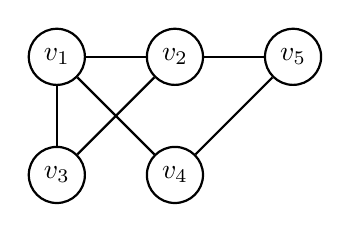
\begin{tikzpicture}[node distance={15mm}, thick, main/.style = {draw, circle}]
        \node[main] (1) {$v_1$};
        \node[main] (2) [right of=1] {$v_2$};
        \node[main] (3) [below of=1] {$v_3$};
        \node[main] (4) [below of=2] {$v_4$};
        \node[main] (5) [right of=2] {$v_5$};
        \draw (1) -- (2);
        \draw (1) -- (3);
        \draw (1) -- (4);
        \draw (2) -- (3);
        \draw (2) -- (5);
        \draw (4) -- (5);
    \end{tikzpicture}
    \caption{Undirected graph}
    \label{f_graphs_undirected}
\end{subfigure}
\begin{subfigure}[b]{0.45\textwidth}
    \centering
    % TikZ code for the second graph
    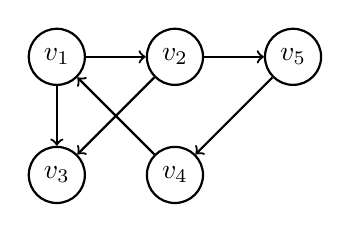
\begin{tikzpicture}[node distance={15mm}, thick, main/.style = {draw, circle}]
        \node[main] (1) {$v_1$};
        \node[main] (2) [right of=1] {$v_2$};
        \node[main] (3) [below of=1] {$v_3$};
        \node[main] (4) [below of=2] {$v_4$};
        \node[main] (5) [right of=2] {$v_5$};
        \draw[->] (1) -- (2);
        \draw[->] (1) -- (3);
        \draw[->] (4) -- (1);
        \draw[->] (2) -- (3);
        \draw[->] (2) -- (5);
        \draw[->] (5) -- (4);
    \end{tikzpicture}
    \caption{Directed graph}
    \label{f_graphs_directed}
\end{subfigure}
\par\bigskip
\begin{subfigure}[b]{0.45\textwidth}
    \centering
    % TikZ code for the first graph
    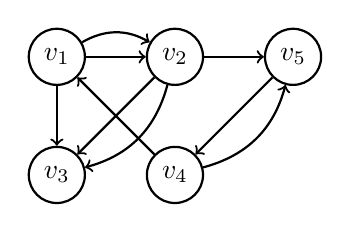
\begin{tikzpicture}[node distance={15mm}, thick, main/.style = {draw, circle}]
        \node[main] (1) {$v_1$};
        \node[main] (2) [right of=1] {$v_2$};
        \node[main] (3) [below of=1] {$v_3$};
        \node[main] (4) [below of=2] {$v_4$};
        \node[main] (5) [right of=2] {$v_5$};
        \draw[->] (1) -- (2);
        \draw[->] (1) to[bend left] (2);
        \draw[->] (1) -- (3);
        \draw[->] (4) -- (1);
        \draw[->] (2) -- (3);
        \draw[->] (2) to[bend left] (3);
        \draw[->] (2) -- (5);
        \draw[->] (5) -- (4);
        \draw[->] (4) to[bend right] (5);
    \end{tikzpicture}
    \caption{Multigraph}
    \label{f_graphs_multi}
\end{subfigure}
\begin{subfigure}[b]{0.45\textwidth}
    \centering
    % TikZ code for the second graph
    \begin{tikzpicture}[node distance={15mm}, thick, main/.style = {draw, circle}]
        \node[main] (1) {$v_1$};
        \node[main] (2) [right of=1] {$v_2$};
        \node[main] (3) [below of=1] {$v_3$};
        \node[main] (4) [below of=2] {$v_4$};
        
        \node[draw, rectangle, left=1mm of 1] {$f_{v_1}=[...]$};
        \node[draw, rectangle, right=1mm of 2] {$f_{v_2}=[...]$};
        \node[draw, rectangle, left=1mm of 3] {$f_{v_3}=[...]$};
        \node[draw, rectangle, right=1mm of 4] {$f_{v_4}=[...]$};
        
        \draw (1) -- (2);
        \draw (1) -- (3);
        \draw (4) -- (1);
        \draw (2) -- (3);
    \end{tikzpicture}
    \caption{Attributed graph}
    \label{f_graphs_attributed}
\end{subfigure}
\par\bigskip
\begin{subfigure}[b]{0.45\textwidth}
    \centering
    % TikZ code for the first graph
    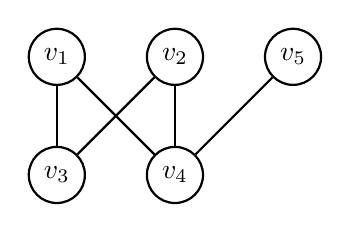
\begin{tikzpicture}[node distance={15mm}, thick, main/.style = {draw, circle}]
        \node[main] (1) {$v_1$};
        \node[main] (2) [right of=1] {$v_2$};
        \node[main] (3) [below of=1] {$v_3$};
        \node[main] (4) [below of=2] {$v_4$};
        \node[main] (5) [right of=2] {$v_5$};
        
        \draw (1) -- (3);
        \draw (1) -- (4);
        \draw (2) -- (3);
        \draw (2) -- (4);
        \draw (4) -- (5);
    \end{tikzpicture}
    \caption{Bipartite graph}
    \label{f_graphs_bipartite}
\end{subfigure}
\begin{subfigure}[b]{0.45\textwidth}
    \centering
    % TikZ code for the second graph
    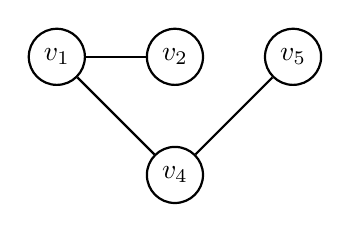
\begin{tikzpicture}[node distance={15mm}, thick, main/.style = {draw, circle}]
        \node[main] (1) {$v_1$};
        \node[main] (2) [right of=1] {$v_2$};
        \node[main] (4) [below of=2] {$v_4$};
        \node[main] (5) [right of=2] {$v_5$};
        \draw (1) -- (2);
        \draw (4) -- (1);
        \draw (5) -- (4);
    \end{tikzpicture}
    \caption{Subgraph of graph (a)}
    \label{f_graphs_subgraph}
\end{subfigure}    
    % Add more subfigures as needed
    \caption{Examples of different graphs. Graphs (a) to (e) exhibit different characteristics, and graph (f) is a subgraph of the undirected graph (a).}
    \label{f_graphs}
\end{figure}

Another critical aspect of graph theory is the concept of subgraphs. A graph $G' = (V', E')$ is called a subgraph of $G = (V,E)$ if $V' \subseteq V$ and $E' \subseteq E$ \cite{diestel_graph_2017}. For example, Figure \ref{f_graphs_subgraph} portrays a subgraph derived from the graph in Figure \ref{f_graphs_undirected}. 

%In the application of functions on graphs, an important type of a subgraph is the local neighborhood of a node. - Not really a subgraph though
In addition to the structural definitions of graphs, there are further graph-related concepts that are important in the scope of this work. A fundamental concept is the local neighborhood $N_1(v_i) = \{v_j \in V | (v_i, v_j) \in E\}$ of a node $v_i \in V$, which consists of those nodes that are adjacent to $v_i$.
%For a node $v_i \in V$, the local neighborhood $N_1(v_i) = \{v_j \in V | (v_i, v_j) \in E\}$ \cite{wu_comprehensive_2021} consists of those nodes adjacent to $v_i$. 
The local neighborhood $N_1(v_i)$ is also referred to as the $1$-hop-neighborhood of $v_i$ because it exclusively contains nodes at a distance of $1$ edge from $v_i$ \cite{bronstein_geometric_2021}. More broadly, the $k$-hop-neighborhood $N_k(v_i)$ of a node $v_i$ encompasses nodes connected to $v_i$ by walks with a length of at most $k$. 

% Wrap up by transitioning to static graphs

%As previously discussed, graphs provide a foundational framework for representing relationships between objects. Describing these connections as sets of nodes and edges allows modeling data from many different domains and with various shapes and forms \cite{bronstein_geometric_2017, kazemi_representation_2019}. Such graphs are commonly known as static graphs \cite{kazemi_representation_2019, rossi_temporal_2020, you_roland_2022} because they capture relationships that remain constant. 

The graphs presented up to this point are commonly referred to as static graphs \cite{kazemi_representation_2019, rossi_temporal_2020, you_roland_2022} because they capture relationships that remain constant. However, the real world rarely remains static; it continuously evolves, adapts, and undergoes change. To address the need for modeling these dynamic transformations, the concepts of static graphs are extended by a temporal dimension to encompass so-called dynamic graphs. Dynamic graphs introduce the element of time, allowing the capture of how relationships evolve and persist over time. In doing so, they provide a richer, more nuanced understanding of interconnected systems, closely mirroring real-world processes \cite{you_roland_2022, xu_inductive_2020, trivedi_dyrep_2019}. Examples of real-world processes that are best modeled as dynamic graphs are social networks, in which connections between individuals constantly form and end, and road networks with traffic information that continuously changes.

Two main approaches for modeling dynamic graphs have been proposed: First, modeling evolving graphs as a series of different static snapshots of a graph, so-called \acrfullpl{dtdg} \cite{he_explainer_2022, xie_explaining_2022}. Second, modeling dynamic graphs as a timed list of interaction events, so-called \acrfullpl{ctdg} \cite{rossi_temporal_2020, trivedi_dyrep_2019}. In the following sections, these approaches are explored to establish the foundation of this work.

\subsubsection{Discrete-Time Dynamic Graphs}
\label{s_Background_Graphs_DTDGs}
\glspl{dtdg} represent dynamic graphs as a series of static graph snapshots captured at different points in time \cite{rossi_temporal_2020}. These snapshots are usually taken with a constant temporal distance \cite{souza_provably_2022}. The changes between the snapshots represent the dynamic evolution of the graph. Formally, a dynamic graph in discrete-time representation is defined as $\mathcal{G} = \{G_t | t = 1,...,T\}$, where $T$ denotes the number of timestamps for which a snapshot is recorded \cite{you_roland_2022}. Each snapshot represents a static graph $G_t = (V_t, E_t)$ with a set of nodes $V_t = \{v \in V | \tau_v = t\}$ and a set of edges $E_t = \{e \in E | \tau_e = t\}$ at a specific time $t \in \{1, ..., T\}$. Each vertex $v$ and edge $e$ carries a timestamp $\tau_v$ and $\tau_e$ respectively \cite{you_roland_2022}. $V$ and $E$ represent the sets of nodes and edges aggregated across all timestamps. Furthermore, in an attributed \gls{dtdg} each snapshot is associated with node features $A_t^{vertex} = \{a_{v,t}^{vertex} | v \in V_t\}$ and edge features $A_t^{edge} = \{a_{e,t}^{edge} | e \in E_t\}$. Compared to its static counterpart, the temporal $1$-hop-neighborhood $N_1(v_i, t) = \{v_j \in V_t | (v_i, v_j) \in E_t\}$ of a node $v_i \in V$ additionally depends on the time $t$. Using the \gls{dtdg} representation, node and edge additions and deletions, as well as attribute updates to node and edge features can be modeled. Figure \ref{f_dtdg} shows an example of a \gls{dtdg}.


\begin{figure}[h]
    \centering
\begin{subfigure}[b]{0.3\textwidth}
    \centering
    % TikZ code for the first graph
    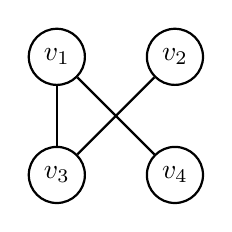
\begin{tikzpicture}[node distance={15mm}, thick, main/.style = {draw, circle}]
        \node[main] (1) {$v_1$};
        \node[main] (2) [right of=1] {$v_2$};
        \node[main] (3) [below of=1] {$v_3$};
        \node[main] (4) [below of=2] {$v_4$};
        \draw (1) -- (3);
        \draw (1) -- (4);
        \draw (2) -- (3);
    \end{tikzpicture}
    \caption{Snapshot $G_1$}
    \label{f_dtdg_1}
\end{subfigure}
\begin{subfigure}[b]{0.3\textwidth}
    \centering
    % TikZ code for the second graph
    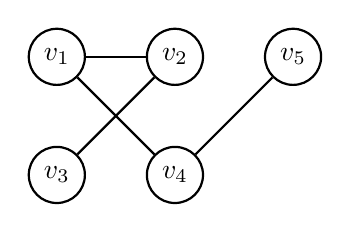
\begin{tikzpicture}[node distance={15mm}, thick, main/.style = {draw, circle}]
        \node[main] (1) {$v_1$};
        \node[main] (2) [right of=1] {$v_2$};
        \node[main] (3) [below of=1] {$v_3$};
        \node[main] (4) [below of=2] {$v_4$};
        \node[main] (5) [right of=2] {$v_5$};
        \draw (1) -- (2);
        \draw (1) -- (4);
        \draw (2) -- (3);
        \draw (4) -- (5);
    \end{tikzpicture}
    \caption{Snapshot $G_2$}
    \label{f_dtdg_2}
\end{subfigure}
\begin{subfigure}[b]{0.3\textwidth}
    \centering
    % TikZ code for the second graph
    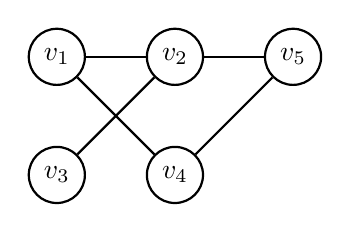
\begin{tikzpicture}[node distance={15mm}, thick, main/.style = {draw, circle}]
        \node[main] (1) {$v_1$};
        \node[main] (2) [right of=1] {$v_2$};
        \node[main] (3) [below of=1] {$v_3$};
        \node[main] (4) [below of=2] {$v_4$};
        \node[main] (5) [right of=2] {$v_5$};
        \draw (1) -- (2);
        \draw (1) -- (4);
        \draw (2) -- (3);
        \draw (2) -- (5);
        \draw (4) -- (5);
    \end{tikzpicture}
    \caption{Snapshot $G_3$}
    \label{f_dtdg_3}
\end{subfigure}
    % Add more subfigures as needed
    \caption{Example of a \gls{dtdg} $\mathcal{G}=\{G_1, G_2, G_3\}$ at different snapshots. Between $G_1$ and $G_2$ the edge $\{v_1, v_3\}$ is removed, node $v_5$ is added and edges $\{v_1, v_2\}$ and $\{v_4, v_5\}$ are added. From $G_2$ to $G_3$ another edge $\{v_2, v_5\}$ is added.}
    \label{f_dtdg}
\end{figure}

While \glspl{dtdg} offer simplicity and ease of processing through their snapshot-based representation \cite{kazemi_representation_2019}, they sacrifice detailed structural information by design, leading to a coarse depiction of temporal data \cite{trivedi_dyrep_2019, kazemi_representation_2019}. Consequently, they may struggle to capture small and irregular temporal changes \cite{trivedi_dyrep_2019, souza_provably_2022}. For example, this representation may miss the addition and prompt removal of an edge. Moreover, selecting an appropriate granularity for taking snapshots often results in suboptimal representations \cite{trivedi_dyrep_2019}. Reducing the time interval between snapshots can mitigate these limitations. Still, it introduces complexity by including the entire static graph in each snapshot, leading to parameter redundancy due to shared nodes and edges between snapshots. These shortcomings are addressed by \acrlongpl{ctdg}.

\subsubsection{Continuous-Time Dynamic Graphs}
\label{s_Background_Graphs_CTDGs}

\glspl{ctdg} offer a high temporal granularity \cite{trivedi_dyrep_2019} and are efficiently represented as sequence of timestamped events $\mathcal{G} = \{\varepsilon_{1}, \varepsilon_{2}, ...\}$ \cite{rossi_temporal_2020}. Following Rossi et al. \cite{rossi_temporal_2020}, each event $\varepsilon_{i}$ is associated with a timestamp $t_i$ with $t_1 \leq t_2 \leq ...$. 
There are node-wise events and interaction events. A node-wise event expresses the addition, removal, or attribute update of a node. Node-wise events are defined as a tuple:

\begin{equation}
    \varepsilon_{i} = (v_j, a^{vertex}_{v_j, t_i}, type_{i}, t_i)
\end{equation}

The tuple contains a timestamp $t_i$ that denotes the time at which the event happens. Further, it includes an event type ${type_{i} \in \{\mathrm{add}, \mathrm{delete}, \mathrm{update}\}}$ that describes what the event represents, e.g., either a node addition, a node deletion, or a feature update for a node. Additionally, it includes the node $v_j$ that is added, deleted, or updated, as well as its node features $a^{vertex}_{v_j, t_i}$ at that point in time. As example, the event $\varepsilon_1 = (v_1, (1,1,1), \mathrm{add}, t_1)$ describes the addition of node $v_1$ with attributes $(1,1,1)$ to the graph at time $t_1$.

An interaction event represents the addition, removal, or attribute update of an edge. Interaction events are defined as a tuple:

\begin{equation}
    \varepsilon_{i} = (e_j, a^{edge}_{e_j, t_i}, type_{i}, t_i)
\end{equation}

Similar to node-wise events, interaction events are also associated with a timestamp $t_i$ that denotes the time of the occurrence of the interaction event and an event type ${type_{i} \in \{\mathrm{add}, \mathrm{delete}, \mathrm{update}\}}$ that defines what type of an event $\varepsilon_i$ is. Interaction events include an edge $e_j$ that is part of the interaction, as well as the attributes of this edge $a^{edge}_{e_j, t_i}$. As an example, the event $\varepsilon_5 = (e_1, (1,1,1), \mathrm{add}, t_5)$ with $e_1 = (v_1, v_2)$ describes the addition of an edge $e_1$ between nodes $v_1$ and $v_2$ with attributes $(1,1,1)$ to the dynamic graph at time $t_5$.

%There are node-wise events and interaction events. A node-wise event $\varepsilon_{i} = (v_j, a^{vertex}_{v_j, t_i}, type_{i}, t_i)$ is a tuple that expresses a node addition, deletion, or feature update. The tuple contains the features of node $v_j$ at $t_i$ denoted by $a^{vertex}_{v_j, t_i}$. A node-wise event additionally is associated with an event type $type_{i} \in \{\mathrm{add}, \mathrm{delete}, \mathrm{update}\}$ that describes what the event represents. An interaction event $\varepsilon_{i} = (e_j, a^{edge}_{e_j, t_i}, type_{i}, t_i)$ signifies the addition, deletion, or feature update of an edge $e_j$. An interaction event includes the associated edge features $a^{edge}_{e_j, t_i}$ of edge $e_j$ at timestamp $t_i$ and an event type $type_{i}$. 
Depending on whether an event $\varepsilon_i$ is a node-wise event or an interaction event, it has one or two so-called involved nodes. The involved node in a node-wise event is the node that the event adds, deletes, or updates. The involved nodes in an interaction event are those two nodes that are connected by the edge that is added, deleted, or updated by the event. 

The node set $V$ and the edge set $E$ include all nodes and edges that are involved in any event in $\mathcal{G}$. A snapshot $G_{t_i} = (V_{t_i}, E_{t_i})$ of a \gls{ctdg} $\mathcal{G}$ is a representation of $\mathcal{G}$ at time $t_i$ as a static graph. $V_{t_i}$ is the node set and $E_{t_i}$ the edge set in the snapshot $G_{t_i}$. The snapshot $G_{t_i}$ at time $t_i$ is constructed from all events $\mathcal{G}(t_i) = \{\varepsilon_1, \varepsilon_2, ..., \varepsilon_i\}$ that occurred before or at timestamp $t_i$.

% For any timestamp $t_i$ a snapshot $G_{t_i}$ of $\mathcal{G}$ at that particular time is defined by all past events $\mathcal{G}(t_i) = \{\varepsilon_{j} | j = 1,...,i\}$.

As in \glspl{dtdg}, the temporal $1$-hop-neighborhood of a node $v_i \in V$ at time $t_l$ is defined as $N_1(v_i, t_l) = \{v_j \in V_{t_l} | (v_i, v_j) \in E_{t_l}\}$. The temporal-$k$-hop-neighborhood consists of those nodes $v_j \in V_{t_l}$ that are connected to $v_i$ with a walk in $E_{t_l}$ that has a length of at most $k$.

%The concept of temporal neighborhoods is extended from nodes to events. The temporal $k$-hop-neighborhood $N_k(\varepsilon_i)$ of an event $\varepsilon_{i}$ consists of those events $\varepsilon_{j} \in \mathcal{G}(t_i) \setminus \varepsilon_{i}$ for which any node involved in event $\varepsilon_{i}$ is in the temporal $k$-hop-neighborhood of any node involved in the event $\varepsilon_{j}$.

For \glspl{ctdg}, the concept of temporal neighborhoods is extended from nodes to events. The temporal $k$-hop-neighborhood $N_k(\varepsilon_i)$ of an event $\varepsilon_{i}$ consists of those past events that involve nodes that are in the temporal $k$-hop-neighborhood of the nodes involved in the event $\varepsilon_{i}$. This means an event $\varepsilon_{j} \in (\mathcal{G}(t_i) \setminus \varepsilon_{i})$ is in the temporal $k$-hop-neighborhood of $\varepsilon_{i}$ if any node involved in event $\varepsilon_{i}$ is in the temporal $k$-hop-neighborhood of any node involved in the event $\varepsilon_{j}$.

\vspace{5mm}

Table \ref{t_ctdg_events} and Figure \ref{f_ctdg} illustrate an example of a \gls{ctdg} $\mathcal{G}$, showing the events in Table \ref{t_ctdg_events} and the evolving graph in Figure \ref{f_ctdg}. Table \ref{t_ctdg_events} demonstrates that this representation provides a highly detailed yet compact representation of the dynamic graph evolution. This is a significant advantage over the representation as \gls{dtdg} \cite{trivedi_dyrep_2019}. The drawback of \glspl{ctdg} is that an evaluation of the graph's state at any given timestamp necessitates the examination of all past events and the assembly of the graph at that specific moment. In comparison, the snapshots that comprise a \gls{dtdg} already have a graph structure.

\begin{table}[ht]
    \centering
    \begin{tabular}{|l|l|}
        \hline
        Event & Description \\
        \hline
        $\varepsilon_{1} = \{v_1, a^{vertex}_{v_1, t_1}, \mathrm{add}, t_1\}$ & Add vertex $v_1$\\
        $\varepsilon_{2} = \{v_2, a^{vertex}_{v_2, t_2}, \mathrm{add}, t_2\}$ & Add vertex $v_2$\\
        $\varepsilon_{3} = \{v_3, a^{vertex}_{v_3, t_3}, \mathrm{add}, t_3\}$ & Add vertex $v_3$\\
        $\varepsilon_{4} = \{e_1 = \{v_1, v_3\}, a^{edge}_{e_1, t_4}, \mathrm{add}, t_4\}$ & Add edge $e_1$ between vertices $v_1$ and $v_3$\\
        $\varepsilon_{5} = \{e_2 = \{v_2, v_3\}, a^{edge}_{e_2, t_5}, \mathrm{add}, t_5\}$ & Add edge $e_2$ between vertices $v_3$ and $v_3$\\
        $\varepsilon_{6} = \{v_4, a^{vertex}_{v_4, t_6}, \mathrm{add}, t_6\}$ & Add vertex $v_4$\\
        $\varepsilon_{7} = \{e_1 = \{v_1, v_3\}, a^{edge}_{e_1, t_7}, \mathrm{delete}, t_7\}$ & Remove edge $e_i$ between vertices $v_1$ and $v_3$\\
        $\varepsilon_{8} = \{v_1, a^{vertex}_{v_1, t_8}, \mathrm{delete}, t_8\}$ & Remove vertex $v_1$\\
        $\vdots$ & $\vdots$ \\
    \end{tabular}
    \caption{Sequence of events comprising an example graph $\mathcal{G}.$}
    \label{t_ctdg_events}
\end{table}

\begin{figure}[ht]
    \centering
\begin{subfigure}[b]{0.3\textwidth}
    \centering
    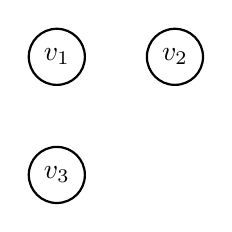
\begin{tikzpicture}[node distance={15mm}, thick, main/.style = {draw, circle}]
        \node[main] (1) {$v_1$};
        \node[main] (2) [right of=1] {$v_2$};
        \node[main] (3) [below of=1] {$v_3$};
    \end{tikzpicture}
    \caption{$G_{t_3}$}
    \label{f_ctdg_1}
\end{subfigure}
\begin{subfigure}[b]{0.3\textwidth}
    \centering
    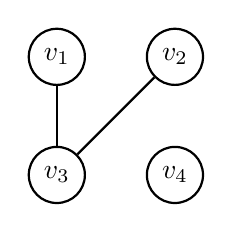
\begin{tikzpicture}[node distance={15mm}, thick, main/.style = {draw, circle}]
        \node[main] (1) {$v_1$};
        \node[main] (2) [right of=1] {$v_2$};
        \node[main] (3) [below of=1] {$v_3$};
        \node[main] (4) [below of=2] {$v_4$};
        \draw (1) -- (3);
        \draw (2) -- (3);
    \end{tikzpicture}
    \caption{$G_{t_6}$}
    \label{f_ctdg_2}
\end{subfigure}
\begin{subfigure}[b]{0.3\textwidth}
    \centering
    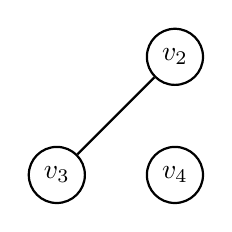
\begin{tikzpicture}[node distance={15mm}, thick, main/.style = {draw, circle}]
        \node[main] (3) {$v_3$};
        \node[main] (4) [right of=3] {$v_4$};
        \node[main] (2) [above of=4] {$v_2$};
        \draw (2) -- (3);
    \end{tikzpicture}
    \caption{$G_{t_8}$}
    \label{f_ctdg_3}
\end{subfigure}
    \caption{Different example snapshots of the graph $\mathcal{G}$ from Table \ref{t_ctdg_events} at timestamps $t_3$, $t_6$ and $t_8$.}
    \label{f_ctdg}
\end{figure}


\subsection{Geometric Deep Learning}
\label{s_Background_GeometricDeepLearning}


A major hurdle for applying deep learning methods to graphs lies in their underlying non-euclidean structure \cite{wu_comprehensive_2021}. This means that graph data cannot be mapped to an Euclidean space $\mathbb{R}^n$ (for some dimension $n$). Geometric deep learning extends deep neural networks to non-Euclidean domains, providing a framework for working with graph data \cite{bronstein_geometric_2017, bronstein_geometric_2021}. The core principle in geometric deep learning is to leverage inherent symmetries in data to improve the performance of deep learning approaches \cite{bronstein_geometric_2021}. These inherent symmetries are used as inductive biases for deep models, which means that the models are designed in such a way that they can take advantage of the symmetries \cite{bronstein_geometric_2021}. Symmetries are transformations of the input data that leave the underlying structure and relationships in the data unchanged \cite{bronstein_geometric_2021}. These transformations can include translations, rotations, reflections, and other geometric operations \cite{bronstein_geometric_2021}. When the output of a function remains unchanged for symmetric data instances, it is referred to as invariant to that transformation \cite{bronstein_geometric_2017}. For instance, an image classification model that is invariant to rotations recognizes an object in an image regardless of its orientation. 

% A symmetry refers to the invariance of specific properties of a system to transformations \cite{bronstein_geometric_2021}. An invariance is a property of a model that remains unchanged under certain transformations. For instance, an image classification model that is invariant to rotations recognizes an object in an image regardless of its orientation. 


The key structural property that provides a symmetry in graphs is that nodes in a graph are provided without a fixed order \cite{bronstein_geometric_2021}. This means that the output of functions on graphs should be independent of the order of the nodes \cite{bronstein_geometric_2021}. A function that satisfies this condition is called a permutation invariant function \cite{bronstein_geometric_2021}. An example of a permutation invariant function on a set of numbers is the arithmetic mean function, which provides the same output regardless of the order of the numbers in the set.

Deep learning methods that apply permutation invariant functions to graph data are referred to as \acrfullpl{gnn} \cite{bronstein_geometric_2021}. The following section covers the specifics of how these models translate the findings of geometric deep learning to actual deep neural models.





%The nature of traditional deep learning methods often presents challenges when applied to graph data due to its non-Euclidean characteristics \cite{wu_comprehensive_2021}. That is because even though universal approximation theorems show that sufficiently complex neural networks can approximate diverse high dimensional functions \cite{hornik_multilayer_1989, kratsios_non-euclidean_2020}, finding a good fit in a general neural network is not trivial and gets increasingly difficult with growing neural network sizes \cite{bronstein_geometric_2021}. This problem is referred to as the curse of dimensionality \cite{bellman_dynamic_1966}. Many deep learning techniques have been able to overcome the curse of dimensionality and excelled because they use inductive biases to help the model process data with a specific structure, mostly with Euclidean or grid-like structural organization \cite{bronstein_geometric_2017}. \textit{Geometric deep learning} extends deep neural models to non-Euclidean domains, including unstructured sets, manifolds, and graphs, leveraging their underlying geometry for inductive biases \cite{bronstein_geometric_2017, bronstein_geometric_2021}.
%%To address the need for generalizing deep neural models to non-Euclidean domains, the field of \textit{geometric deep learning} emerges, extending the power of deep learning to domains such as unstructured sets, manifolds, and graphs using their underlying geometry for inductive biases \cite{bronstein_geometric_2017, bronstein_geometric_2021}.

%Geometric deep learning leverages the geometric principles of symmetry, deformation stability, and scale separation to aid deep learning models in learning complex functions \cite{bronstein_geometric_2021}. Symmetry refers to the invariance of specific properties of (physical) systems to transformations \cite{bronstein_geometric_2021}. For instance, in computer vision, object categorization remains unaffected by shifts to images, making shifts a form of symmetry \cite{bronstein_geometric_2021}. Using symmetries as is cannot properly aid deep learning models since exact symmetries are rare in real world data, which usually exhibits a significant degree of noise \cite{bronstein_geometric_2021}. Thus, the principle of deformation stability relaxes the definition of invariance and introduces the notion of similarity between data points \cite{bronstein_geometric_2021}. Deformation stability suggests that to maintain a similar representation for data instances that differ through slight distortions, feature mappings must demonstrate a type of stability \cite{bronstein_geometric_2021}. Lastly, encoding data in a multi-scale, hierarchical manner enables the detection of complex correlations \cite{bronstein_geometric_2021}. Multi-scale decomposition splits the learned function into elementary functions that capture the different facets and hierarchical nature of much data \cite{bronstein_geometric_2021}. Combining these principles provides the basis for learning stable representations of high-dimensional data.

%The critical structural property for applying geometric deep learning to graphs is that the nodes in a graph are assumed to be provided without a fixed order, meaning that the output of functions on graphs should not depend on the ordering of nodes \cite{bronstein_geometric_2021}. This is called \textit{permutation invariance} \cite{bronstein_geometric_2021}. For example, the sum function is a permutation-invariant function that aggregates values over all nodes \cite{bronstein_geometric_2021}, providing a graph-wise output. However, the focus of many tasks on graphs, like node classification of link prediction, is node-wise information, requiring functions that act locally \cite{bronstein_geometric_2021}. Such functions are realized by applying permutation invariant functions over local neighborhoods of the investigated nodes \cite{bronstein_geometric_2021}. 

%Approaches that apply these results to deep learning on graphs are referred to as \glspl{gnn}. The following section covers how these models translate the findings of geometric deep learning to actual deep neural models.

%%The nature of traditional deep learning methods often presents challenges when applied to graph data due to its non-Euclidean characteristics \cite{wu_comprehensive_2021}. Unlike data with inherent Euclidean attributes, such as a vector space structure, an underlying coordinate system, or shift invariance, graph data lacks these essential properties \cite{bronstein_geometric_2017}. Many deep learning techniques have excelled on data that possesses an inherent Euclidean or grid-like structural organization \cite{bronstein_geometric_2017}. To address the need for generalizing deep neural models to non-Euclidean domains, the field of \textit{geometric deep learning} emerges, extending the power of deep learning to domains such as unstructured sets, manifolds, and graphs \cite{bronstein_geometric_2017, bronstein_geometric_2021}.

%% What should I put here exactly? I want to bridge the gap to graph neural networks so it should introduce only the necessary background for that, thus maybe first state the general principle and then what that means for gnns? General principle: "exposing the regularities in data through unified geometric principles that can be applied throughout a wide spectrum of applications"

\subsection{Graph Neural Networks}
\label{s_Background_GNNs}


% Transition from GDL to GNNs. Make a short introduction and later cover how the GDL principles show in the different architectures.

\glspl{gnn} are potent tools for various learning tasks on relational and interaction data. They find successful applications in many domains, including drug discovery \cite{dauparas_robust_2022}, weather forecasting \cite{lam_graphcast_2022}, and reasoning on knowledge graphs \cite{huang_few-shot_2022}. 
%They achieve this performance by exploiting the properties of the permutation group underlying graph data \cite{bronstein_geometric_2021}.

The applications of \glspl{gnn} are diverse, but their tasks are often similar. The common tasks are node, edge, and graph classification, node regression, and link prediction \cite{wu_comprehensive_2021, zhou_graph_2020}.
\begin{itemize}
    \item \textbf{Node, Edge, and Graph classification} are the tasks of learning a function that maps each node, edge, or graph to their corresponding label \cite{kipf_semi-supervised_2017}.
    \item \textbf{Node regression} involves predicting a continuous numerical value associated with a node \cite{wu_comprehensive_2021}.
    \item \textbf{Link prediction} is the task of predicting the presence or absence of edges between pairs of nodes \cite{liben-nowell_link-prediction_2007}.
\end{itemize}

To accomplish these tasks, \glspl{gnn} typically learn representations for elements of graphs, like nodes and edges \cite{zhou_graph_2020}. Learning these representations allows the models to understand and use the structural information present in graph-structured data. The following sections lay out a generalized view of \glspl{gnn} and present \glspl{gnn} as an encoder-decoder pair.

\subsubsection{Encoder-Decoder Framework}
\label{s_Background_GNNs_EncoderDecoderFramework}

Different existing approaches to \glspl{gnn} use diverse notations and conceptualizations to describe their methodologies. This thesis follows \cite{hamilton_representation_2017} and \cite{kazemi_representation_2019} in describing \glspl{gnn} as an encoder-decoder pair.
%Addressing the diversity in notation and methodology followed by different existing approaches to \glspl{gnn}, this thesis follows \cite{hamilton_representation_2017} and \cite{kazemi_representation_2019} in describing \glspl{gnn} as an encoder-decoder pair. 
In the encoder-decoder framework, the so-called encoder component produces representations for graph elements, referred to as embeddings. The decoder is then tasked with making predictions based on these embeddings. Depending on the graph and task, nodes, edges, relation types, subgraphs, and/or entire graphs are embedded \cite{barros_survey_2023}. In many cases, embeddings are only calculated for nodes. Thus, in the following, only node embeddings are discussed. Within the encoder-decoder framework, node embeddings are formally defined as: 

\begin{definition}
    \label{d_Embedding}
    An \textbf{Embedding} is a numerical representation $h_v$ for a node $v \in V$ in a graph. This representation commonly consists of one or more numerical scalars, vectors, or matrices \cite{kazemi_representation_2019}. For a given graph $G = (V, E)$, node embeddings are the result of the embedding function $emb: (v, G) \mapsto h_v \hspace{5pt} \forall v \in V$.
\end{definition}

Embeddings should capture and represent the structural and semantic information of nodes, facilitating information propagation, integrating local and global features, and enabling effective graph reasoning in downstream tasks \cite{goyal_graph_2018}. The embedding function $emb$ should thus provide similar embeddings for nodes that have structurally and semantically similar neighborhoods and similar features \cite{goyal_graph_2018, bronstein_geometric_2021}.
%The embedding function $emb$ should thus preserve a sense of proximity defined on the graph \cite{goyal_graph_2018}. 
Often, embeddings take the form of a single vector $h_v \in \mathbf{R}^d$ that has a significantly lower dimensionality than the number of nodes in the graph $d<<|V|$ \cite{goyal_graph_2018}. 

%The encoder and decoder are defined formally as follows:

%\begin{definition}
%    \label{d_Encoder}
%    Given an input graph $G$, the \textbf{Encoder} is the embedding function that maps each node $v \in V$ to an embedding $h_v$.
%    \begin{equation}
%        h_v = emb(v, G)
%    \end{equation}
%\end{definition}

%Oftentimes, the encoder produces embeddings in the form of a single vector $Emb_v = (z_v), z_v \in \mathbf{R}^{n}$ \cite{kazemi_representation_2019}. 
Within the encoder-decoder framework, the encoder refers to the node embedding function $emb$. The encoder typically builds on top of geometric deep learning principles and includes trainable parameters, such as neural network layers or modules. There are many different architectural variants for encoders, which are discussed in more detail in Section \ref{s_Background_GNNs_GNNArchtectures}. In contrast, the decoder component is formally defined as:

\begin{definition}
    \label{d_Decoder}
    Given an embedding $h_v$ produced by the embedding function $emb$, the decoder makes predictions $y$ for a particular task.
    \begin{equation}
        y = Decoder(h_v)
    \end{equation}
\end{definition}

Like the encoders, decoders often incorporate trainable parameters \cite{hamilton_representation_2017}. The decoder architecture depends on the desired output format and the task it handles \cite{hamilton_representation_2017}. In link prediction, for example, the decoder may predict the likelihood of the existence of an edge, given the embeddings of the nodes in the predicted edge.

\subsubsection{Graph Neural Network Architectures}
\label{s_Background_GNNs_GNNArchtectures}

Fundamental differences in \glspl{gnn} architectures arise in the encoder. While the exact realization of the encoder can be diverse, most approaches build upon the same foundational structure \cite{bronstein_geometric_2021}. \glspl{gnn} are structured in so-called \gls{gnn} layers \cite{bronstein_geometric_2021, wu_comprehensive_2021, zhou_graph_2020}. Each node $v_i \in V$ in a graph is associated with a representation $h_{v_i}^l$ that is updated by each of the layers in the \gls{gnn} \cite{bronstein_geometric_2021}. The representation usually comes in the form of a numeric vector. A \gls{gnn} layer is a computational step that updates the representation of each node in a graph by aggregating information from neighboring nodes \cite{wu_comprehensive_2021}. 
\gls{gnn} layers operate on the graph structure, and the node features $A^{vertex}$ of a graph $G$ \cite{bronstein_geometric_2021}. In each layer, a shared permutation invariant function $\sigma$ is applied to local neighborhoods $N_1(v_i)$ of each node $v_i \in V$ \cite{bronstein_geometric_2021}. The output of this permutation invariant function for a node $v_i \in V$ in the $l$-th layer of a \gls{gnn} is an updated representation $h_{v_i}^l$ of $v_i$. Consecutive \gls{gnn} layers use the updated node representations produced by their preceding layers as input to the permutation invariant function $\sigma$. In doing so, they aggregate information from outside the local neighborhoods into the representations of each node. The first layer uses the raw node features $h_{v_i}^0 = a^{vertex}_{v_i}, \forall v_i \in V$ as input \cite{hamilton_representation_2017}. If the nodes have no features, the initial representation is commonly initialized with random values \cite{wu_comprehensive_2021}. The updated node representation that is output by the last layer of a \gls{gnn} is the embedding $h_{v_i}$ of a node. On a generalized level, \glspl{gnn} obtain updated node representations in the $l$-th layer as:

%\gls{gnn} layers operate on the adjacency matrix $A$, and the node features $A^{vertex}$ of a graph $G$ \cite{bronstein_geometric_2021}. Each layer applies a permutation equivariant function $F(A^{vertex}, A)$ by subjecting local neighborhoods $N_1(v_i)$ for each node $v_i \in V$ to a shared permutation invariant function $\sigma$ \cite{bronstein_geometric_2021}. This results in updated features $h_{v_i}^l$ as output of the $l$-th layer of a \gls{gnn}. Consecutive \gls{gnn} layers use the updated node features of previous layers, allowing the aggregation of information from outside the immediate neighborhood of the nodes. The first layer uses the raw node features $h_{v_i}^0 = a^{vertex}_{v_i}, \forall v_i \in V$ as input \cite{hamilton_representation_2017}. On a generalized level, \glspl{gnn} obtain updated node features as:

\begin{equation}
    h_{v_i}^l = \sigma(h_{v_i}^{l-1}, \underset{v_j \in N_1(v_i)}{\oplus} \psi(h_{v_j}^{l-1}, \cdots))
\end{equation}

Here, permutation invariance is achieved by aggregating the features of the local neighborhood $N_1(v_i)$ of node $v_i \in V$ from the previous layer with a permutation invariant function $\oplus$. For example, this can be the sum, mean, or maximum function \cite{bronstein_geometric_2021}. The function $\psi$ is dependent on the exact \gls{gnn} implementation and it represents the main differentiating factor of \gls{gnn} architectures. $\psi$ is applied to each node $v_j$ in the local neighborhood of $v_i$. It takes the updated features $h_{v_j}^{l-1}$ from the previous \gls{gnn} layer as input alongside other implementation-specific features.

Following Bronstein et al. \cite{bronstein_geometric_2021}, most \gls{gnn} architectures are derived from one of three types of \gls{gnn} layers. These layer types are mainly differentiated by how the permutation invariant function $\sigma$ transforms the neighborhood features through different realizations of $\psi$.

\begin{itemize}
    \item \textbf{Convolutional \glspl{gnn}:} In this architecture, information from the local neighborhood is directly aggregated with fixed weights $c_{v_i, v_j}$ that represent the importance of node $v_j$ to the representation of a node $v_i$ \cite{bronstein_geometric_2021, wu_comprehensive_2021}.
    \begin{equation}
        h_{v_i}^l = \sigma(h_{v_i}^{l-1}, \underset{v_j \in N_1(v_i)}{\oplus} c_{v_i, v_j} \varphi(h_{v_j}^{l-1}))
    \end{equation}
    
    \item \textbf{Attention-based \glspl{gnn}:} By assigning different weights to neighboring elements, attention-based operators can alleviate noise and enhance the quality of results \cite{zhou_graph_2020}. Weights result from a learnable self-attention mechanism $a$ \cite{bronstein_geometric_2021}.
    \begin{equation}
        h_{v_i}^l = \sigma(h_{v_i}^{l-1}, \underset{v_j \in N_1(v_i)}{\oplus} a(h_{v_i}^{l-1}, h_{v_j}^{l-1}) \varphi(h_{v_j}^{l-1}))
    \end{equation}

    \item \textbf{Message-passing-based \glspl{gnn}:} This architecture treats graph layers as a message-passing process in which nodes directly pass information to their neighbors \cite{wu_comprehensive_2021}. A learnable message function $\varphi$ passes information between neighboring nodes \cite{bronstein_geometric_2021}.
    \begin{equation}
        h_{v_i}^l = \sigma(h_{v_i}^{l-1}, \underset{v_j \in N_1(v_i)}{\oplus} \varphi(h_{v_i}^{l-1}, h_{v_j}^{l-1}))
    \end{equation}
\end{itemize}

$\sigma$ and $\psi$ usually are learnable functions \cite{bronstein_geometric_2021}. The node embeddings are typically obtained as the updated node features from the final layer of a \gls{gnn} \cite{hamilton_representation_2017}. These embeddings are then used as input to task-specific decoders \cite{hamilton_representation_2017}. The exact implementations for these decoders vary and depend on the task performed by the \gls{gnn}.

\subsection{Temporal Graph Neural Networks}
\label{s_Background_TGNNs}

Compared with static \glspl{gnn}, \acrfullpl{tgnn} introduce representations for the temporal dimension of evolving data. Existing \gls{tgnn} approaches are differentiated by the dynamic graph representation they target. Some approaches target \glspl{dtdg} \cite{sankar_dysat_2020, manessi_dynamic_2020, you_roland_2022}, while others target \glspl{ctdg} \cite{rossi_temporal_2020, souza_provably_2022, ma_streaming_2018}.
%Existing approaches for \glspl{tgnn} are differentiated by those that work on \glspl{dtdg} and those that work on \glspl{ctdg}. 
Many approaches combine \gls{gnn} layers developed for static \glspl{gnn} with \glspl{cnn} or \glspl{rnn} to introduce a temporal dimension \cite{wu_comprehensive_2021}. In general, \gls{tgnn} methods learn time-dependent node-embeddings \cite{longa_graph_2023}. They are structured into layers, similar to static \glspl{gnn}. The output of the last layer of a \gls{tgnn} for a node $v_i$ at time $t_j$ is the time-dependent node-embeddings $h_{v_i}(t_j)$.
%These outputs of the last layer of a \gls{tgnn} are considered as such node-embeddings and are referred to as $h_{v_i}(t_j)$, representing the embedding of node $v_i \in V$ at time $t_j$.
The following sections generalize common \gls{tgnn} approaches for both types of temporal graph representations with a unified notation.

\subsubsection{Temporal Graph Neural Networks for Discrete Time Dynamic Graphs}
\label{s_tgnns_for_dtdgs}
\glspl{tgnn} for \glspl{dtdg} combine an approach for handling snapshots of the entire graph at each time point with a mechanism for learning temporal dependencies across time steps \cite{longa_graph_2023}. The most common approach is to evolve embeddings produced by a static \gls{gnn} over time \cite{longa_graph_2023}. Hence, a permutation invariant function $\sigma$, which is adapted from the permutation invariant function in static \glspl{gnn}, is employed in this context. Formally, this function is adjusted to calculate updated features of node $v_i \in V$ at a given time $t \in \{1,...,T\}$ as follows:

\begin{equation}
    \sigma(h_{v_i}^{l-1}(t), \underset{v_j \in N_1(v_i, t)}{\oplus} \psi(h_{v_j}^{l-1}(t), \cdots))
\end{equation}

$\psi$ is an implementation-specific function that may take additional features as input. As in static \glspl{gnn}, different architectures can be realized through different implementations of $\psi$. For each timestep $t$, $\sigma$ functions exactly the same way as its counterpart in static \glspl{gnn}, using the snapshot $G_t$ of the dynamic graph at time $t$ as a basis.

$\sigma$ is combined with a temporal update function $\phi$ to obtain the updated node features \cite{you_roland_2022}.
\begin{equation}
    h_{v_i}^l(t) = \phi(h_{v_i}^{l}(t-1), \sigma(h_{v_i}^{l-1}(t), \underset{v_j \in N_1(v_i, t)}{\oplus} \psi(h_{v_j}^{l-1}(t), \cdots)))
\end{equation}
The temporal update function $\phi$ encodes the temporal dynamics by including the node representation of the last timestep $h_{v_i}^{l}(t-1)$ \cite{longa_graph_2023}. The update function might take additional arguments, depending on the specific implementation. There exist various implementations of the permutation invariant function $\sigma$ and the temporal update function $\phi$ \cite{longa_graph_2023}. These include using self-attention \cite{sankar_dysat_2020}, or \glspl{rnn} like a \gls{gru} \cite{you_roland_2022}.

\subsubsection{Temporal Graph Neural Networks for Continuous Time Dynamic Graphs}
\label{s_tgnns_for_ctdgs}
\gls{tgnn} methods for \glspl{ctdg} effectively handle sequences of events by integrating methods that refresh a node's representation whenever an event related to that node takes place \cite{longa_graph_2023}. They represent an extension of static \glspl{gnn} because they merge and aggregate node representations within temporal neighborhoods \cite{longa_graph_2023}.

While the exact approaches vary significantly \cite{longa_graph_2023}, a relatively generic framework is \gls{tgn} \cite{rossi_temporal_2020}. Since many popular approaches are specific instances of \gls{tgn} \cite{trivedi_dyrep_2019, rossi_temporal_2020} or extend upon it \cite{souza_provably_2022}, the following paragraphs describe \glspl{tgnn} for \glspl{ctdg} from the viewpoint of the \gls{tgn} framework.

\glspl{tgnn} for \glspl{ctdg} introduce two novel concepts: 
Event-specific messages and node-specific state. 
Each node $v_i \in V$ is associated with a time-dependent state vector $s_{v_i}(t)$ that represents all its past interactions \cite{longa_graph_2023}. Whenever an event $\varepsilon_{k}$ that involves node $v_i \in V$ occurs, a message $m_{v_i}(\varepsilon_{k})$ is generated to update the node's state $s_{v_i}(t_k)$. For an interaction event $\varepsilon_{k}$ between source node $v_i \in V$ and target node $v_j \in V$, it is possible to compute two messages:
\begin{equation}
    m_{v_i}(\varepsilon_{k}) = msg_s(s_{v_i}(t_k^-), s_{v_j}(t_k^-), \varepsilon_{k}), \hspace{15pt} m_{v_j}(\varepsilon_{k}) = msg_t(s_{v_j}(t_k^-), s_{v_i}(t_k^-), \varepsilon_{k})
\end{equation}
$t_k^-$ refers to the time just before $t_k$, meaning that $s_{v_i}(t_k^-)$ is the state of node $v_i$ just before the event $\varepsilon_{k}$ occurs. This formulation distinguishes between source and target nodes to represent directed graphs. Thus, separate message functions exist for updates to the source node state $msg_s$ and the target node state $msg_t$.
To update the node state in undirected graphs, both message functions are used to update each node with both the source node message $msg_s$ and the target node message $msg_t$. In the case that the encountered event $\varepsilon_{k}$ is a node-wise event on node $v_i \in V$, a single message is computed:
\begin{equation}
    m_{v_i}(\varepsilon_{k}) = msg_n(s_{v_i}(t_k^-), \varepsilon_{k})
\end{equation}

The message functions $msg_s, msg_t, msg_n$ can be learnable. A message $m_{v_i}(\varepsilon_{k})$ updates the state $s_{v_i}(t_k)$ of node $v_i$ trough a learnable state function $state$:
\begin{equation}
    s_{v_i}(t_k) = state(m_{v_i}(\varepsilon_{k}), s_{v_i}(t_k^-))
\end{equation}

The $state$ function is a \gls{rnn}, often in the form of a \gls{lstm} or \gls{gru} \cite{longa_graph_2023}.
The state is used to compute node embeddings in the \gls{tgnn} layers. These layers resemble their counterparts from static \glspl{gnn}. On a generalized level, updated node features at time $t$ are calculated as:
\begin{equation}
    h_{v_i}^l(t) = \sigma(h_{v_i}^{l-1}(t), \underset{v_j \in N_1(v_i, t)}{\oplus} \psi(s_{v_j}(t), \cdots))
\end{equation}

Where $\sigma$ and $\psi$ can be learnable \cite{rossi_temporal_2020}. $\psi$ takes the state of neighboring nodes as input, together with other features, depending on the specific implementation. Like in static \glspl{gnn}, the actual mechanisms used in the permutation invariant function vary. Popular approaches include using \glspl{rnn} \cite{ma_streaming_2018} and a self-attention mechanism \cite{rossi_temporal_2020}.

To improve scalability, modern \glspl{tgnn} for \glspl{ctdg} employ strategies like only updating the state periodically with an aggregated version of the messages \cite{rossi_temporal_2020}. There also exist approaches that do not use a separate state component. Instead, they embed nodes directly by combining node features, graph topology, and time embeddings \cite{longa_graph_2023, xu_inductive_2020}, similar to static \glspl{gnn}.




\iffalse
\gls{tgn} have been proposed by \cite{rossi_temporal_2020} and represent a general framework for learning representations in dynamic graphs. The framework consists of different modules

\begin{itemize}
    \item \textbf{Memory.} The purpose of the memory module is to store long-term dependencies specific to each node within the graph. The memory at time $t$ represents each node $v_i$ it has already seen as a vector $s_i(t)$. When a node is first encountered, it is initialized with the zero vector. The memory of node $v_i$ is always updated when an event involving that node occurs, for example, an interaction with another node or an update to the node features of $v_i$.
    \item \textbf{Message Function.} For each event $e_i$ a memory update message is computed for each node involved in $e_i$. For example, in the case of an edge addition even $e_i$, introducing an edge between $I_i = \{v_j, v_k\}$, a memory update message is computed for both nodes $v_j$ and $v_k$. In the case of an interaction event between two nodes $e_i = ((v_j, v_k), t_i, a_i)$ the update message is calculated as
    \begin{center}
        $m_j(t_i) = msg_{src}(s_j(t_i^-), s_k(t^-), \Delta t, a_i)$, $m_k(t_i) = msg_{tgt}(s_k(t_i^-), s_j(t^-), \Delta t, a_i)$.
    \end{center}
    In the case of a node-wise event $e_i = ((v_j), t_i, a_i)$ it is calculated as
    \begin{center}
        $m_j(t_i) = msg_{node}(s_i(t_i^-), t_i, a_i)$.
    \end{center}
    $s_j(t_i^-)$ denotes the memory of node $v_j$ just before time $t_i$, $\Delta t$ refers to the time difference between the last memory update and $t_i$. The functions $msg_{src}, msg_{tgt}, msg_{node}$ can be learnable like a Multilayer perceptron. However, the original TGN model uses a simple concatenation of the inputs.
    \item \textbf{Message Aggregator.} The message aggregator enables batch processing of events. Since one batch consists of events until some time $t$ can include multiple events that involve any node $v_i$, this produces multiple memory update messages $m_i(t_1),...,m_i(t_b)$ for $t_1,...,t_b \leq t$ for that node. The message aggregator aggregates these messages into a single aggregated update message
    \begin{center}
        $\bar{m}_i(t) = agg(m_i(t_1), ..., m_i(t_b))$.
    \end{center}
    The aggregation function $agg$ can be learnable, for example, realized as \gls{rnn}. However, the original TGN model uses one of two simple strategies: Aggregate as only the most recent message or aggregate as the mean of all update messages.
    \item \textbf{Memory Updater.} The memory updated uses the (aggregated) update message $\bar{m}_i(t)$ to update the memory of a node $v_i$.
    \begin{center}
        $s_i(t) = mem(\bar{m}_i(t), s_i(t^-))$
    \end{center}
    $mem$ is a learnable function realized as \gls{rnn}, for example as \gls{lstm} or \gls{gru}.
    \item \textbf{Embedding.} The embedding module produces temporal embeddings $z_i(t)$ for node $v_i$ at time $t$. Because the memory of node $v_i$ is only updated when it partakes in an event, its memory could have become outdated if there were no events involving $v_i$ for an extended period of time. The embedding module circumvents this problem by not providing the memory of a node as embedding but instead computing it as
    \begin{center}
        $z_i(t) = emb(v_i,t) = \sum_{n_j \in \mathcal{N}^k_i([0,t])} h(s_i(t), s_j(t), a_{ij}, ???)$
    \end{center}
    with $h$ being a learnable function.
\end{itemize}
\fi


%Add something on XAI? Maybe would make sense if the problem formulation is undertaken next and not in the methodology section
\section{Explaining deep graph models}
\label{s_ExplainingGNNs}

%No longer purely related work. First outline explainable ai in general, then transition to gnns and the cummulate into the next chapter on explanability methods on gnns. Last part of the chapeter is the related work subchapter

% Introduction into related work, laying out the general story of the chapter: From explanations on static graphs and the different approaches to more detailed description of highly related work on explanations on dynamic graphs

Alongside the rise in adaptation of artificial intelligence and deep learning methods over recent years, the idea of explainable artificial intelligence has been gaining increasing attention \cite{adadi_peeking_2018}. The field of explainable artificial intelligence focuses on providing transparency over the mechanisms that underlie artificial models \cite{barredo_arrieta_explainable_2020}. Many machine learning models behave like black-boxes, meaning that the internal mechanisms that lead to their predictions remain opaque to their users \cite{prado-romero_survey_2023}. Explainable artificial intelligence differentiates \textit{interpretability} from \textit{explainability}.
Interpretability refers to the degree to which the internal workings and decision-making processes of an artificial intelligence model can be understood by humans by design \cite{barredo_arrieta_explainable_2020}.
In comparison, explainability refers to the ability of an artificial intelligence system to provide clear, coherent, and accessible explanations for its decisions or predictions, offering insights into the rationale behind specific outcomes in a human-understandable manner \cite{barredo_arrieta_explainable_2020}. While interpretable \gls{gnn} models utilize mechanisms that are easy to understand on their own \cite{prado-romero_survey_2023}, black-box \gls{gnn} models have shown better performance on high-dimensional input data than interpretable models \cite{prado-romero_survey_2023}. Thus, proper explanation methods are required to make black-box models explainable.

%Transition to explanability for gnns and outline the structure of this chapter.

Even though most works on static \glspl{gnn} have only emerged in the past 10 years \cite{wu_comprehensive_2021}, the black-box nature of the majority of these \glspl{gnn} has given rise to a plethora of explanation methods. The explanation approaches that have been proposed vary in many ways, like the type of explanation provided, the mechanism by which they explain produce explanations, or if and how explainers are trained \cite{kakkad_survey_2023}. Figure \ref{f_taxonomy_explainers} provides a classification of these varied approaches. On a conceptual level, model-level and instance-level approaches are differentiated \cite{yuan_explainability_2020}. Model-level methods explain \glspl{gnn} as a whole, irrespective of any particular input example \cite{yuan_explainability_2020}. Such explanations aim to uncover a high-level understanding of the inner workings of the explained \gls{gnn}. In comparison, instance-level methods explain the output of a model for a specific input instance \cite{yuan_explainability_2020}. These explanations are tailored to individual instances, offering a fine-grained understanding of the reasoning behind each prediction.

\begin{figure}[ht]
    \centering
    \tikzset{
  basic/.style  = {draw, rectangle},
  root/.style   = {basic, thin, align=center},
  level 2/.style = {basic, thin, align=center, sibling distance=60mm, text width=10em},
  level 3/.style = {basic, thin, align=center, sibling distance=30mm, text width=10em},
  level 4/.style = {basic, thin, align=center, text width=7.5em}
}
\begin{tikzpicture}[level 1/.style={sibling distance=90mm}, edge from parent/.style={->,draw}, >=latex]
    \node[root] {\gls{gnn} Explanations}
        child {node[level 2] (c1) {Instance level}
            child {node[level 3] (c3) {Factual}}
            child {node[level 3] (c4) {Counterfactual}}
        }
        child {node[level 2] (c2) {Model level}};

    \begin{scope}[every node/.style={level 4}]
        \node[below of = c3, xshift=15pt] (c31) {Gradient};
        \node[below of = c31] (c32) {Decomposition};
        \node[below of = c32] (c33) {Surrogate};
        \node[below of = c33] (c34) {Perturbation};

        \node[below of = c4, xshift=15pt] (c41) {Search based};
        \node[below of = c41] (c42) {Heuristic based};
        \node[below of = c42] (c43) {Learning based};

        \node[below of = c2, xshift=15pt] (c21) {Generation};
    \end{scope}

    \foreach \value in {1,...,4}
        \draw[->] (c3.188) |- (c3\value.west);
    \foreach \value in {1,2,3}
        \draw[->] (c4.188) |- (c4\value.west);
    \foreach \value in {1}
        \draw[->] (c2.188) |- (c2\value.west);
\end{tikzpicture}
    \caption{Taxonomy of \gls{gnn} explanation methods. Explanation approaches are categorized into instance-level and model-level methods. The category of instance-level methods is further subdivided into factual and counterfactual approaches. Taxonomy adapted from \cite{yuan_explainability_2020}, \cite{prado-romero_survey_2023}, and \cite{kakkad_survey_2023}.}
    \label{f_taxonomy_explainers}

\end{figure}

\textit{Model-level} explainers like XGNN \cite{yuan_xgnn_2020} map the behavior of a \gls{gnn} to patterns in the input graphs \cite{yuan_explainability_2020}. These explainers use a so-called generation approach, which explains \glspl{gnn} by training a model to generate graphs that maximize a particular prediction of the \gls{gnn} \cite{yuan_explainability_2020, yuan_xgnn_2020}. The thereby generated graph patterns are then used as an explanation \cite{yuan_xgnn_2020}. While these approaches can provide high-level explanations for the general model behavior, they fail to explain the specifics of why certain predictions are made for given inputs and are thus not discussed any further.

\textit{Instance-level} approaches are subdivided into those that provide a factual and those that provide a counterfactual explanation. On a fundamental level, factual reasoning inquires, "With A already having occurred, will B occur?" \cite{quelhas_relation_2018, tan_learning_2022}. Hence, a factual explanation states that a prediction for B was made because A occurred. In contrast, counterfactual reasoning poses the question, "If A did not occur, would B still happen?" \cite{quelhas_relation_2018, tan_learning_2022}. A counterfactual explanation is thus interested in the information A, whose non-existence would entail a different prediction for the occurrence of B. The following sections take a closer look at explanation methods using either type of reasoning.

\subsection{Factual Explanation Approaches}
\label{s_ExplainingGNNs_Factual}

Factual explanations for \glspl{gnn} answer the question: "Given the input A, will the \gls{gnn} predict B?". These explanations seek the input information with the maximum influence on the \gls{gnn}'s prediction \cite{kakkad_survey_2023}. They can take the form of a subgraph $G' \subseteq G$ of the original input $G$ \cite{kakkad_survey_2023} that is \textit{sufficient} to produce the original prediction with the targeted \gls{gnn} $f(\cdot)$ \cite{tan_learning_2022}. For a sufficient factual explanation, the following equation holds:

\begin{equation}
    f(G) = f(G')
\end{equation}

\vspace{0.5cm}

As depicted in Figure \ref{f_taxonomy_explainers}, Factual explainers for \glspl{gnn} are categorized based on the primary mechanisms they employ to explain predictions, each offering different approaches and forms of explanations:

\begin{itemize}
    \item \textbf{Gradient/Feature} based methods identify important features by analyzing how changes in input features affect the network's predictions \cite{yuan_explainability_2020}. These approaches either employ back-propagation to examine the gradients of the explained prediction concerning the input features or map hidden features through interpolation into the input space \cite{yuan_explainability_2020}. Examples of these methods are Class Activation Mapping (CAM)\cite{pope_explainability_2019} and Sensitivity Analysis (SA) \cite{baldassarre_explainability_2019}.
    
    \item \textbf{Decomposition} methods break down a \gls{gnn}'s prediction into contributions from individual nodes or edges by creating score decomposition rules through back-propagation \cite{yuan_explainability_2020}. These rules attribute the prediction scores to individual features in the input space \cite{yuan_explainability_2020, baldassarre_explainability_2019}. Notable decomposition approaches are Layer-wise Relevance Propagation (LRP) \cite{baldassarre_explainability_2019} and \gls{gnn}-LRP \cite{schnake_higher-order_2022}.
    
    \item \textbf{Surrogate} methods create a separate, easy-to-interpret model to approximate the behavior of a \gls{gnn} on data similar to the explained example \cite{yuan_explainability_2020}. Usually, neighboring data to the explained example is sampled and used to train easily analyzable models \cite{huang_graphlime_2023} like linear regression models \cite{duval_graphsvx_2021} or Bayesian networks \cite{vu_pgm-explainer_2020}. Relevant publications that leverage surrogate models for explanations are Probabilistic Graphical Model Explainer (PGM-Explainer) \cite{vu_pgm-explainer_2020} and Graph Local Interpretable Model Explanations (GraphLIME) \cite{huang_graphlime_2023}.
    
    \item \textbf{Perturbation}-based methods analyze how the output of a \gls{gnn} model changes when the input is perturbed \cite{yuan_explainability_2020}. Input perturbations refer to alterations to the input graphs \cite{yuan_explainability_2020}. Perturbation-based methods usually create feature masks that highlight those input features that are important for the prediction and exclude the unimportant features \cite{yuan_explainability_2020, ivanovs_perturbation-based_2021}. Perturbation-based methods operate with either a learning-based or a search-based perturbation approach \cite{xia_explaining_2023}. Popular learning-based perturbation approaches are GNNExplainer \cite{ying_gnnexplainer_2019} and PGExplainer \cite{luo_parameterized_2020}. GNNExplainer \cite{ying_gnnexplainer_2019} uses a trainable model to generate masks for the input features, which requires training for each explained prediction separately. In contrast, PGExplainer \cite{luo_parameterized_2020} uses a trainable masking model that is only trained once for a graph and can then be applied to explain any prediction on that graph. In terms of search-based perturbation approaches, SubgraphX \cite{yuan_explainability_2021} is an influential method that uses Monte Carlo tree search to find perturbations that explain a prediction.
\end{itemize}

While gradient/feature and decomposition approaches require direct access to the internal model parameters or embeddings by design, some surrogate and perturbation-based methods can operate without such access \cite{kakkad_survey_2023}. Needing direct access is a disadvantage since it requires adaptations in the explainer before these methods can be applied to new models. It also prohibits the application of the explainers to models that do not expose their inner workings.

As mentioned description of the explanation mechanisms, perturbation-based methods use either a learning-based or a search-based perturbation approach \cite{xia_explaining_2023}. Both of these approaches usually generate a perturbed subgraph of the original input graph, which serves as an explanation. Learning-based approaches identify the most critical features of the input graph by feeding the node embeddings and/or edge embeddings produced by the explained \gls{gnn} into a learnable model that extracts a perturbed subgraph \cite{kakkad_survey_2023, xia_explaining_2023}. The \gls{gnn} predictions on this subgraph are then compared to the original predictions with a distance function, providing a score that serves as training input for the subgraph extraction model \cite{kakkad_survey_2023}. Search-based perturbation approaches generate modified subgraphs from the original input using heuristic search algorithms together with a game-theoretical scoring function \cite{xia_explaining_2023, yuan_explainability_2021}. A clear advantage of the search-based perturbation strategy is that model access is only needed on the level of predictions, not for the embeddings. This comes at the cost of longer inference times \cite{xia_explaining_2023} since the search-based approach requires the separate exploration of various input perturbations for each explained instance \cite{yuan_explainability_2021}.

% Write something to put these methods into perspective. For example a disctinction between search- and learning-based perturbation approaches should be included since I refer to it in the related work section

% Idea would be to compare these 4 approaches and to discuss their most interesting characteristics and shortcomings. I wonder if it makes sense to actually detail the inner workings of any particular explainer or not because it is only inderectly relevant to my thesis

\subsection{Counterfactual Explanation Approaches}
\label{s_ExplainingGNNs_CounterFactual}

Counterfactual explanations for \glspl{gnn} answer the question, "What changes in the input graph are necessary to change the prediction produced by a \gls{gnn} model?". Counterfactual explanations aim to identify so-called counterfactual examples. A counterfactual example consists of the smallest possible alteration to the input information such that the model prediction changes \cite{kakkad_survey_2023}. These counterfactual examples consist of the input information that is \textit{necessary} to the prediction of the explained model \cite{tan_learning_2022}. If the information contained in a counterfactual example is excluded from the input, the prediction of the explained model changes \cite{tan_learning_2022}. Counterfactual explanations for \glspl{gnn} have risen in attention over the last years \cite{ma_clear_2022} for their ability to produce intuitive explanations \cite{ma_clear_2022}, offer feedback for non-experts \cite{prado-romero_survey_2023}, foster trust in \glspl{gnn} \cite{prado-romero_survey_2023}, and help in addressing model biases \cite{prado-romero_survey_2023}. Further, they are useful for identifying potential adversarial examples that could be used to attack models \cite{lucic_cf-gnnexplainer_2022}.

Typically, counterfactual examples consist of a subgraph $\mathcal{X} \subseteq G$ which if removed from the input graph $G$ will result in the explained \gls{gnn} $f(\cdot)$ producing a different prediction than on the full original graph $G$ \cite{tan_learning_2022}:
\begin{equation}
    \label{e_cf_explanation}
    f(G) \neq f(G\setminus \mathcal{X})
\end{equation}

In some cases, counterfactual examples also include information added to the original graph $G$ \cite{abrate_counterfactual_2021}. In such instances, the definition of counterfactual examples is extended. In this extended definition a counterfactual example $\mathcal{X} = \{\mathcal{X}^-, \mathcal{X}^+\}$ consist of a graph $\mathcal{X}^- \subseteq G$, containing information removed from $G$, and a graph $\mathcal{X}^+ = (V^+, E^+)$ with ${v_i \in V^+ \implies v_i \notin V}$ and $e_i \in E^+ \implies e_i \notin E$ that contains information added to the input graph. This combination must satisfy the following equation:

\begin{equation}
    f(G) \neq f((G \cup \mathcal{X}^+) \setminus \mathcal{X^-})
\end{equation}

All counterfactual explanation methods leverage a perturbation-based approach. Similar to the perturbation approaches for factual explanations, a difference between search-based and learning-based approaches is made.

%Counterfactual explainers fall into three high-level methods that differ in how they seek alterations in the input graph to create counterfactual explanations.

\begin{itemize}
    \item \textbf{Search-based} approaches either explore alterations to the input graph dependent on a specific criterion \cite{prado-romero_survey_2023}, like a similarity measure between separate alterations of a graph \cite{abrate_counterfactual_2021}, or they use a systematic policy for modifying the input graph until they attain a valid counterfactual \cite{prado-romero_survey_2023}. Examples of this type of counterfactual explainers are Molecular Model Agnostic Counterfactual Explanations (MMACE) \cite{wellawatte_model_2022} and Oblivious Backward Search (OBS) \cite{abrate_counterfactual_2021}.
    %\item \textbf{Search based} approaches explore alterations to the input graph dependent on a specific criterion \cite{prado-romero_survey_2023}, like a similarity measure between graph alterations \cite{abrate_counterfactual_2021}, to find a counterfactual example.
    %\item \textbf{Heuristic based} methods depend on a systematic policy for modifying the input graph until they attain a valid counterfactual \cite{prado-romero_survey_2023}. For instance, they may alter the original input by randomly dropping and adding edges until the prediction of the \gls{gnn} changes as done by  \cite{abrate_counterfactual_2021}.
    \item \textbf{Learning based} approaches examine how the \gls{gnn} output changes to variations in the input graph \cite{prado-romero_survey_2023}. They train a model to perturb input graphs in a way that the output of the targeted model changes \cite{lucic_cf-gnnexplainer_2022}. To find counterfactual examples, the trained model is used to produce multiple perturbations of the input graph while checking if the perturbations constitute counterfactual examples \cite{lucic_cf-gnnexplainer_2022}. Various approaches within this category differ in how they create and update the input graph mask and how the model is trained \cite{prado-romero_survey_2023}. A popular representative of this category is CF-GNNExplainer \cite{lucic_cf-gnnexplainer_2022}.
\end{itemize}

There also exist methods that are not fully captured by this classification. For example, RCExplainer \cite{bajaj_robust_2021} combines a learning-based approach with a learned model of the decision logic of a \gls{gnn}.

Counterfactual explainers and \glspl{gnn} are usually decoupled from each other \cite{prado-romero_survey_2023}. Hence, the majority of counterfactual explanation methods for \glspl{gnn} offer the advantage of being model agnostic.

% Make the case for cf explanations over f explanations

\subsection{Comparison of Factual and Counterfactual Approaches}
\label{s_ExplainingGNNs_Comparison}

In comparison, while factual explanations shed light on why a \gls{gnn} makes a particular prediction given the input, counterfactual explanations go a step further by revealing precisely what changes in the input are needed to alter that prediction. Because factual reasoning seeks sufficient information as an explanation for a prediction, it may include redundant information \cite{tan_learning_2022}. In contrast, as counterfactual reasoning only seeks necessary information as explanation, it may only extract a small subset of the information that is actually responsible for the prediction \cite{tan_learning_2022}. For this reason, some works integrate factual and counterfactual reasoning into a single explanation method, for example, CF² \cite{tan_learning_2022}. This has the advantage of addressing the necessity and sufficiency of explanations within the same framework \cite{tan_learning_2022}.

On their own, counterfactual explanations provide a practical and intuitive way for users to grasp what influences the explained model's output in an actionable manner \cite{lucic_cf-gnnexplainer_2022}. By offering concrete, actionable insights into the model's decision-making process \cite{lucic_cf-gnnexplainer_2022}, they empower individuals to understand, trust, and improve \glspl{gnn} in real-world applications \cite{prado-romero_survey_2023}. Thus, counterfactual explanations bridge the gap between the model's black-box behavior and human interpretability, making them a valuable tool for ensuring transparency and accountability.

\section{Related Work}
\label{s_RelatedWork}

% Argue why we only look at the temporal explanation methods, not at any from the static context. Also need to argue why 

As outlined in Chapter \ref{s_ExplainingGNNs}, numerous methods for explaining \glspl{gnn} on static graphs have been developed. However, these models fall short when applied to temporal graph models, as they fail to capture temporal dependencies in dynamic graphs \cite{xia_explaining_2023, he_explainer_2022}. Additionally, they are unable to support the \gls{dtdg} and \gls{ctdg} representations of dynamic graphs. Particularly, the event-based \gls{ctdg} representation is conceptually substantially different from the static representation of graphs as mere sets of nodes and edges. Yet, only a very limited number of past publications have explored explanation methods that take the dynamic nature of \glspl{tgnn} into account. Understanding existing explainability methods in the context of dynamic graphs is crucial for developing and evaluating novel explanation methods for \glspl{tgnn}. Figure \ref{f_taxonomy_explainers} shows an overview of other works that explain \glspl{tgnn}. The methods used in these explainers mainly adapt findings from explainers in the static setting to the dynamic context. 

\begin{figure}[ht]
    \centering
    \tikzset{
  basic/.style  = {draw, rectangle, font={\small}},
  root/.style   = {basic, thin, align=center, minimum height=0.75cm},
  level 2/.style = {basic, thin, align=center, sibling distance=37.5mm, text width=8em, minimum height=0.75cm},
  level 3/.style = {basic, thin, align=center, sibling distance=30mm, text width=8em, minimum height=0.75cm},
  level 4/.style = {basic, thin, align=center, text width=7.5em, pattern=north west lines, pattern color=lightgray}
}
\begin{tikzpicture}[level 1/.style={sibling distance=80mm}, edge from parent/.style={->,draw}, >=latex]
    \node[root] {\gls{tgnn} Explanations}
        child {node[level 2] (c1) {On \glspl{dtdg}}
            child {node[level 3] (c11) {Surrogate}}
            child {node[level 3] (c12) {Features}}
            child {node[level 3] (c13) {Decomposition}}
        }
        child {node[level 2] (c2) {On \glspl{ctdg}}
            child {node[level 3] (c21) {Perturbation}}
        };

        \begin{scope}[every node/.style={level 4}]
        \node[below of = c11, xshift=0.25em] (c111) {He et al. \cite{he_explainer_2022}};
        \node[below of = c12, xshift=0.25em] (c121) {GCN-SE \cite{fan_gcn-se_2021}};
        \node[below of = c13, xshift=0.25em] (c131) {Liu et al. \cite{liu_differential_2023}};
        \node[below of = c131] (c132) {DGExplainer \cite{xie_explaining_2022}};

        \node[below of = c21, text width=9em, xshift=1em] (c211) {TGNNExplainer \cite{xia_explaining_2023}};
        
    \end{scope}

    \foreach \value in {1}
        \draw[->] (c11.172) |- (c11\value.west);
    \foreach \value in {1}
        \draw[->] (c12.172) |- (c12\value.west);
    \foreach \value in {1,2}
        \draw[->] (c13.172) |- (c13\value.west);
    \foreach \value in {1}
        \draw[->] (c21.172) |- (c21\value.west);
    
\end{tikzpicture}
    \label{f_relatedWork_taxonomy}
    \caption{Overview of related work. Some works focus on explaining \glspl{tgnn} operating on the \gls{dtdg} representation, while only two other studies explore explanations for \glspl{tgnn} operating on \glspl{ctdg}. The methods are subdivided by their approach, following the taxonomy introduced for the static explanation approaches in Figure \ref{f_taxonomy_explainers}.}
\end{figure}

This chapter provides a structured overview of existing methods and how they compare to the approaches developed in this thesis. Distinguishing the approaches at the level of the underlying graph representation, the following sections outline related works for explanations in the \gls{dtdg} (Section \ref{s_relatedWork_DTDG}) and the \gls{ctdg} setting (Section \ref{s_relatedWork_CTDG}), and then derive the research gap from a comparison of the existing approaches in Section \ref{s_relateWork_comparison}.

\subsection{Explanations on Discrete Time Dynamic Graphs}
\label{s_relatedWork_DTDG}

Most prior work focuses on explanations for predictions on \glspl{dtdg}. Explaining such models involves integrating feature importances over the different graph snapshots \cite{he_explainer_2022}. Existing approaches are based on surrogate models \cite{he_explainer_2022}, temporal decomposition strategies \cite{xie_explaining_2022, liu_differential_2023}, and model features \cite{fan_gcn-se_2021}.

He et al. \cite{he_explainer_2022} adapt PGM-Explainer \cite{vu_pgm-explainer_2020} to explain predictions on \glspl{dtdg}. PGM-Explainer is a surrogate method that aims to construct an optimal Bayesian network that captures the most relevant graph components and provides explanations in the form of conditional probabilities. The authors use PGM-Explainer to explain prediction for individual graph snapshot separately, treating each graph snapshot as a static graph. They subsequently aggregate these individual explanations using a pruning strategy to discover dominant, interesting explanations.

In contrast, GCN-SE \cite{fan_gcn-se_2021} takes a different approach. GCN-SE is a graph convolutional network architecture for \glspl{dtdg} that incorporates attention weights for the different graph snapshots. These attention weights are used to assess the importance of the different snapshots to the final prediction. Thus, the GCN-SE approach provides a degree of self-interpretability. However, the attention weights only offer insights into how important certain snapshots are and not into the importance of features within the snapshot, offering only coarse explanations.

Another category of explanation methods utilizes the decomposition approach. DGExplainer \cite{xie_explaining_2022} decomposes the prediction of a \gls{tgnn} by redistributing the prediction score to relevance scores of neurons in the previous neural network layer. This redistribution is repeated backward through the \gls{tgnn} until the input neurons are reached. This provides importance scores for all input features. Liu et al. \cite{liu_differential_2023} also propose a decomposition-based explanation method. They use standard \glspl{gnn} designed for static graphs to make predictions on the different snapshots. Then, they make the predictions smooth and understandable across the different snapshots using axiomatic attribution. The authors presume that the predicted distributions exist within a low-dimensional manifold. The approach visualizes how these predictions change over time as smooth paths on this manifold. The main goal is to enhance interpretability by finding a path that accurately represents how the predictions change over time.


\subsection{Explanations on Continuous Time Dynamic Graphs}
\label{s_relatedWork_CTDG}

Explanations tailored for \glspl{ctdg} is an area with very limited prior work. Unlike most related works that focus on \glspl{dtdg}, T-GNNExplainer \cite{xia_explaining_2023} and TempME \cite{chen_tempme_2023} use the \gls{ctdg} representation for dynamic graphs. They both use a perturbation approach to provide factual explanations in the form of a subset of past events crucial for the model's predictions.

The underlying perturbation approach of T-GNNExplainer is search-based and leverages Monte Carlo Tree Search to find important events. To improve search performance, the authors introduce a navigator component, a multilayer perceptron trained to predict event importances concerning a given prediction. This navigator informs the exploration of the search space. Notably, T-GNNExplainer differs from many perturbation-based explanation methods in static settings in that it does not require users to specify the size of the explanation. Instead, it autonomously identifies an explanation of an appropriate size. T-GNNExplainer can be interpreted as an adaptation of SubgraphX \cite{yuan_explainability_2021}, a search-based perturbation approach for static \glspl{gnn}, to the dynamic setting. In contrast to this predecessor, T-GNNExplainer uses spatial and temporal constraints for its search space and adopts the navigator component for efficient search space explorations.

In contrast, TempME is an approach that aims to identify crucial temporal motifs to elucidate the reasoning behind predictions. Temporal motifs are recurrent and statistically significant temporal substructures. TempME selects important temporal motifs sampled from a local neighborhood of the nodes involved in the explained prediction. For this selection, it uses a \gls{gnn} pretrained on predicting the importance of motifs to the explained prediction. These importance ratings are used as basis to construct explanations that integrate the collective impact of temporal motifs.

% Usually a \gls{tgnn} $f(\cdot)$ that is tasked to predict the occurrence of future links is fed the examined link $\varepsilon_{t_i}$ alongside all past events $\mathcal{G}(t_i)$. However, in T-GNNExplainer only events in the local k-hop-neighborhood of the prediction target $\varepsilon_{t_i}$ are considered. This is a problem because the omission of the events outside the neighborhood events might result in a different prediction $f(\mathcal{G}(t_i), \varepsilon_{t_i}) \neq f(\mathcal{G}(t_i) \cap N^k_{\varepsilon_{t_i}}, \varepsilon_{t_i})$.


\subsection{Comparison}
\label{s_relateWork_comparison}

While the presented related works provide valuable contributions to explaining predictions of \glspl{tgnn}, they display different shortcomings and leave many possible explanation methods unexplored. Table \ref{t_relatedWork_Overview} summarizes the key characteristics of these approaches. 

\begin{table}[ht]
    \centering
    \footnotesize
    \begin{tabular}{ p{3.4cm} >{\centering\arraybackslash} p{2.2cm} >{\centering\arraybackslash} p{2cm} >{\centering\arraybackslash} p{1cm} >{\centering\arraybackslash} p{1.25cm} >{\centering\arraybackslash} p{1.25cm} >{\centering\arraybackslash} p{2cm} }
    \hline
    %Method & \begin{sideways} Dynamic Graph \end{sideways}&\begin{sideways} Tasks \end{sideways}&\begin{sideways} Approach \end{sideways}&\begin{sideways} Model Access \end{sideways}&\begin{sideways} Model Agnostic \end{sideways}&\begin{sideways} CF explanations \end{sideways} \\
    Method & Tasks & Approach & No\newline Model\newline Access & Model\newline Agnostic & \gls{ctdg} & CF\newline explanations\\
    \hline
    He et al. \cite{he_explainer_2022} & NR & Surrogate & \ding{51} & \ding{51} & $\cdot$ & $\cdot$ \\
     %\hline
     GCN-SE \cite{fan_gcn-se_2021} & NC & Features & $\cdot$ & $\cdot$ & $\cdot$ & $\cdot$\\
    %\hline
     Liu et al. \cite{liu_differential_2023} & NC, GC, FLP & Decomposition & $\cdot$ & $\cdot$ & $\cdot$ & $\cdot$ \\
     %\hline
    DGExplainer \cite{xie_explaining_2022} & FLP, NR & Decomposition & $\cdot$ & $\cdot$ & $\cdot$ & $\cdot$ \\
    %\hline
    T-GNNExplainer \cite{xia_explaining_2023} & FLP & Perturbation & $\sim^*$ & \ding{51}* & \ding{51} & $\cdot$ \\
    TempME \cite{chen_tempme_2023} & FLP & Perturbation & \ding{51} & \ding{51} & \ding{51} & $\cdot$ \\
    %\hline
    \textit{\gls{greedycf} (this work)} & FLP & Perturbation & \ding{51} & \ding{51} & \ding{51} & \ding{51}\\
    \textit{\gls{cftgnn} (this work)} & FLP & Perturbation & \ding{51} & \ding{51} & \ding{51} & \ding{51}\\
    \hline
\end{tabular}
    \caption{Overview of related work compared to the explainer proposed in this thesis. The abbreviations for the tasks are Node Regression (NR), Node Classification (NC), Graph Classification (GC), and Future Link Prediction (FLP). *: The navigator component in T-GNNExplainer requires access to attention weights.}
    \label{t_relatedWork_Overview}
\end{table}

\glspl{tgnn} operating on \glspl{ctdg} are generally more versatile than their \gls{dtdg} counterparts because \glspl{dtdg} can be converted into \glspl{ctdg} without loss of information, but not necessarily the other way around \cite{souza_provably_2022}. Nonetheless, explanations for \glspl{tgnn} working on \glspl{ctdg} remain heavily understudied \cite{chen_tempme_2023}. T-GNNExplainer \cite{xia_explaining_2023} and TempME \cite{chen_tempme_2023} are the only approaches yet to explore explanations in the context of this representation.

A major shortcoming of many existing explanation approaches is that they are not model agnostic. A model agnostic explainer applies to any prediction model \cite{prado-romero_survey_2023}; however, most of the related works require a specific class of model, for instance, an attention-based method. This means that such methods cannot be applied to black-box models.

Another factor limiting the applicability of most related explanation approaches is model access. Explanation methods can require access to the prediction model on different levels. Access on the level of gradients, embeddings \cite{verma_counterfactual_2020}, and predictions are differentiated. While approaches that require embedding-wise access only limit the scope of explainable models to those that produce such embeddings, approaches with gradient-wise access restrict the range of explainable models to those that employ neural networks \cite{prado-romero_survey_2023}. A reliance on model access to internal parameters can prohibit the application of an explainer to a novel model, or it might make rigorous adaptations necessary. Novel methods are often designed without any considerations for explainability or specific explainability methods \cite{xia_explaining_2023}, making a non-reliance on model access an asset for an explainer.

Furthermore, none of the existing approaches makes use of counterfactual explanations even though counterfactual explanations have been shown to be highly effective explanations, as they overcome many problems in interpretability and accountability \cite{wachter_counterfactual_2018}. Additionally, counterfactual explanations have already been successfully applied to regular \glspl{gnn} \cite{tan_learning_2022, lucic_cf-gnnexplainer_2022}, but their potential in dynamic graph contexts remains unexplored.

This thesis improves on existing explanation methods for prediction models on dynamic graphs. It addresses the identified research gap by proposing \gls{greedycf} and \gls{cftgnn}, two instance-level post-hoc explainer that provides counterfactual examples as explanations for \glspl{tgnn} operating on \glspl{ctdg}. The proposed methods are model agnostic, treating the explained model as a black-box with model access only required on the level of predictions. Both approaches use a search-based perturbation strategy that seeks to find minimal counterfactual examples. In proposing \gls{greedycf} and \gls{cftgnn}, this thesis advances the current state of explanation methods for dynamic graphs.

% First build some taxonomical overview of the existing methods, then present them and finally in an overview table compare them and outline how the proposed approach improves on different weaknesses and fills the gap in research. Open to debate is where to localise the problem statement because right now it sits before the related work chapter


\section{Problem Formulation}
\label{s_ProblemFormulation}

% Problem Formulation in CF² paper and tgnnexplainer paper as examples
This chapter lays the foundation for exploring the explainability of prediction models on dynamic graphs by formulating the problem of finding counterfactual explanations on \glspl{ctdg}. It introduces the task of future link prediction (Section \ref{s_ProblemFormulation_Task}). This task serves as the reference task for proposing the explanation method. Subsequently, counterfactual explanations are defined for future link prediction (Section \ref{s_ProblemFormulation_CFExamples}). Section \ref{s_ProblemFormulation_Objectives} presents the specific objectives pursued within the explanation approach. Finally, the overall goal of this thesis is summarized in Section \ref{s_ProblemFormulation_ProblemStatement}.

\subsection{Explanations for Future Link Prediction}
\label{s_ProblemFormulation_Task}
In the context of future link prediction, a link prediction model $f: \{\mathcal{G}(t_i), \varepsilon_i\} \rightarrow \mathbbm{R}$ is tasked with predicting whether a future edge addition event $\varepsilon_{i} = \{e_j, a_{e_j, t_i}^{edge}, \mathrm{add}, t_i\}$, referred to as future link, will occur or not. The prediction is based on all events ${\mathcal{G}(t_i) = \{\varepsilon_{l} | \varepsilon_{l} \in \mathcal{G}, t_l \leq t_i\}}$ from the temporal graph $\mathcal{G}$ that happened before or at time $t_i$. Without loss of generality, it is assumed that $f$ provides its prediction in the form of real-valued logits, defined as the quantile function of the standard logistical distribution. The logit values capture the model's confidence in the occurrence of the event. The model $f$ can be any function that fits this description, for example, a \gls{tgnn} trained on future link prediction. In this task, the model $f$ is also referred to as link prediction function. The binary classification function $p: \mathbbm{R} \rightarrow \{0, 1\}$ is applied to the output of the link prediction function $f$ to get the final interpretation of the prediction:

\begin{equation}
    p(f(\mathcal{G}(t_i), \varepsilon_{i})) = 
    \begin{cases}
    1,  &\text{if } f(\mathcal{G}(t_i), \varepsilon_{i}) \geq 0 \\
    0,  &\text{else}
    \end{cases}
\end{equation}

If the classification function outputs a value of $1$, the prediction is classified as a forecast of the future link's occurrence. If it outputs $0$, the prediction is classified as a forecast of the future link's non-occurrence.

%\begin{equation}
%    f(\mathcal{G}(t_i), \varepsilon_{i})=
%    \begin{cases}
%    1,  &\text{if the prediction is that $\varepsilon_{i}$ will occur} \\
%    0,  &\text{if the prediction is that $\varepsilon_{i}$ will not occur}
%    \end{cases}
%\end{equation}
An explainer is a function that provides an explanation for a model's prediction. Within the context of future link prediction, an explainer $ex(\cdot)$ is a function that takes the link prediction function $f$, the explained event $\varepsilon_{i}$, and the list of past events $\mathcal{G}(t_i)$ as input and outputs an explanation for the model's prediction.

While the explanation approach proposed in this thesis primarily focuses on the domain of future link prediction, the insights gained can be generalized to adapt to node and graph classification tasks with minor adjustments.

\subsection{Counterfactual Examples}
\label{s_ProblemFormulation_CFExamples}

As discussed in Section \ref{s_ExplainingGNNs}, counterfactual explanations are a valuable tool for providing intuitive and actionable explanations regarding “why” a specific prediction was made. Thus, they are particularly well-suited for explaining future link predictions made by difficult-to-understand deep graph models like \glspl{tgnn}.

%They are thus particularly well-suited for explaining predictions in the context of future link prediction by difficult-to-understand deep graph models like \glspl{tgnn}.

A counterfactual example $\mathcal{X}_{\varepsilon_i}$ to a model's prediction on the occurrence of a future link $\varepsilon_{i}$ consist of a subset of past events $\mathcal{X}_{\varepsilon_i} \subseteq \mathcal{G}(t_i)$. To be considered counterfactual, the subset has to be necessary to produce the original prediction, satisfying the following condition:

\begin{equation}
    \label{e_CFExplanation}
    p(f(\mathcal{G}(t_i), \varepsilon_{i})) \neq p(f((\mathcal{G}(t_i) \setminus \mathcal{X}_{\varepsilon_i}), \varepsilon_{i}))
\end{equation}

For any potential future link $\varepsilon_{i}$, there may exist multiple counterfactual examples or no counterfactual example at all. The set containing all existing counterfactual examples for a potential future link $\varepsilon_{i}$ is denoted as $\Psi_{\varepsilon_i}$.

A counterfactual explainer for the future link prediction task $ex$ is defined as a function that takes a link prediction function $f$, a temporal graph $\mathcal{G}(t_i)$, and a potential future link $\varepsilon_i$ as input. It outputs a subset of the events from the original input graph as a counterfactual explanation.

\begin{equation}
    \label{e_Explainer}
    ex: \{f, \mathcal{G}(t_i), \varepsilon_i\} \rightarrow \bigcup_{k = 0}^{|(\mathcal{G}(t_i) \setminus \varepsilon_i)|} {(\mathcal{G}(t_i) \setminus \varepsilon_i) \choose k}
\end{equation}

The definition constrains the output of the explainer to any combination of past events. This definition follows the notation in \cite{stanley_enumerative_1986} for representing the set of all permutations of a particular size $k$.

\subsection{Objectives of the Explainer}
\label{s_ProblemFormulation_Objectives}

Explaining future link predictions using counterfactual examples entails two primary objectives:

\begin{enumerate}
    \item \textbf{Maximize Discoveries}: The explainer's first objective is to maximize the proportion of cases in which it successfully identifies a counterfactual example. Every subset of past events could potentially constitute a counterfactual example. Given that the number of possible combinations of past events grows exponentially with the number of past events, it quickly becomes infeasible to explore all possible combinations. Thus, the explainer $ex$ should seek to efficiently identify counterfactual examples, maximizing the instances in which the explanation is necessary to the explained prediction. This is achieved by maximizing the following expression:
    \begin{equation}
        \label{e_maxExplanationRate}
        \frac{1}{\mathcal{G}} \sum_{\varepsilon_{i} \in \mathcal{G}} \mathbbm{1}(ex(f, \mathcal{G}(t_i), \varepsilon_{i}) \in \Psi_{\varepsilon_i})
    \end{equation}
    The indicator function $\mathbbm{1}(ex(f, \mathcal{G}(t_i), \varepsilon_{i}) \in \Psi_{\varepsilon_i})$ returns $1$ if the explainer $ex$ finds a counterfactual example for the given input and returns $0$ otherwise.
    \item \textbf{Minimize Complexity}: When multiple counterfactual examples exist, the explainer should select the most concise yet informative explanation. In line with Occam's razor principle, good explanations should be simple, comprising only the most relevant information \cite{yuan_explainability_2020, tan_learning_2022}. Hence, counterfactual examples should have minimal sizes, as measured by the number of events they contain:
    \begin{equation}
        \label{e_minCFExampleSize}
        \argmin_{\mathcal{X}_{\varepsilon_i}^j \in \Psi_{\varepsilon_i}} |\mathcal{X}_{\varepsilon_i}^j|
    \end{equation}
    where the function $|\mathcal{X}_{\varepsilon_i}^j|$ returns the number of events that comprise explanation $\mathcal{X}_{\varepsilon_i}^j$.
\end{enumerate}

%To pursue the first objective, the explainer $ex(\cdot)$ should maximize the following expression:


%To achieve the second objective, the counterfactual example should have minimal size, as measured by the number of events it contains:

%Every subset of past events could potentially constitute a counterfactual example. Since the number of possible combinations of past events has exponential growth with the number of past events, exploring all combinations quickly gets infeasible. Thus, the explainer seeks to find an counterfactual example in as many cases as possible. Therefore, the primary objective is to maximize the proportion of cases in which an explainer manages to find a counterfactual example.\\
%In the case that there exist multiple counterfactual examples we search for that example that explains the prediction best. Following Occam's razor principle good explanations should be simple \cite{yuan_explainability_2020, tan_learning_2022}, only consisting of the most relevant information. This leads to the second objective that explanations should be as small as possible, thus the counterfactual example should have minimal size. Therefore, the number of events contained in the counterfactual example is minimized:

% Small explanations and stability on the level of the actual explanations; maximum number of found counterfactual examples overall

\subsection{Problem Statement}
\label{s_ProblemFormulation_ProblemStatement}

In summary, this thesis proposes explaining predictions made by \glspl{tgnn} in the context of future link prediction using counterfactual explanations. Given a \gls{ctdg} $\mathcal{G} = \{\varepsilon_{1}, \varepsilon_{2}, ...\}$, and a trained temporal graph model $f$, an explainer $ex$ provides explanations for why the model predicts either the occurrence or non-occurrence of a future link $\varepsilon_{i}$. The explanation consists of a subset of the past events $\mathcal{X}_{\varepsilon_{i}}$.

The primary objectives of a counterfactual explainer are two-fold: maximizing the number of cases in which it successfully identifies a counterfactual example while concurrently minimizing the complexity of the explanation.

\section{Methodology}
\label{s_Methodology}

This chapter addresses the explanation problem defined in Section \ref{s_ProblemFormulation} using two search approaches. As the basis for finding counterfactual examples, Section \ref{s_Methodology_SearchSpace} defines the search space and explores the question of how to structure it in accordance with the objectives defined for explainers. Next, Section \ref{s_Methodology_SelectionStrategies} introduces so-called selection strategies, which provide a heuristic approach to guiding the explainers during the search. Following that, Section \ref{s_Methodology_GreedyCF} presents \gls{greedycf}, which is a simple approach that uses a greedy heuristic for finding counterfactual examples. \gls{greedycf} serves as a capable baseline in this thesis. The subsequent section introduces \gls{cftgnn}, which is a sophisticated search approach that builds upon past findings in reinforcement learning and factual explanation methods.

%To solve the problem defined in Section \ref{s_ProblemFormulation}, this chapter introduces two novel search-based explanation approaches. First, 
%As there are not yet any explanation approaches for models on dynamic graphs, Section \ref{s_Methodology_GreedyBaseline} outlines a simple approach for finding counterfactual examples that serves as a capable baseline in this thesis and for future methods. The subsequent section introduces \acrfull{cftgnn}, which leverages counterfactual examples to provide intuitive and understandable explanations in the context of future link prediction on \glspl{ctdg}


%To solve the problem defined in Section \ref{s_ProblemFormulation}, this chapter introduces \acrfull{cftgnn}, a novel search-based explanation approach developed in this thesis. \gls{cftgnn} leverages counterfactual examples to provide intuitive and understandable explanations in the context of future link prediction on \glspl{ctdg}. This chapter presents the details of \gls{cftgnn}'s design, its components, the rationale behind its development, and how it addresses the previously set objectives.
%Section \ref{s_Methodology_Overview} provides an overview of the foundations of the explanation framework, exploring the search space for counterfactual examples and detailing how \gls{cftgnn} employs a search strategy to find such counterfactual examples. Subsequently, Section \ref{s_Methodology_Search} delves into the inner workings of \gls{cftgnn}, explaining the search algorithm in detail. The search algorithm is supplemented with a so-called selection strategy, which provides a heuristic approach for informing the exploration of the search tree (Section \ref{s_Methodology_Selection}). Finally, Section \ref{s_Methodology_GenericGraphTasks} covers how \gls{cftgnn} is generalized to explain other graph tasks.

\subsection{Search Space}
\label{s_Methodology_SearchSpace}


%\subsection{Overview}
%\label{s_Methodology_Overview}

As outlined in Section \ref{s_ProblemFormulation_Objectives}, a counterfactual example $\mathcal{X}_{\varepsilon_i}$ for the prediction $y_{\varepsilon_i}$ of a link prediction function $f$ on a potential future edge addition event $\varepsilon_i$ from the dynamic graph $\mathcal{G}$, could be any combination of past events $\mathcal{X}_{\varepsilon_i} \subseteq \mathcal{G}(t_i) \setminus \varepsilon_i$. Let $S_{\varepsilon_i}$ denote the set containing all possible combinations of past events\footnote{following the notation of \cite{stanley_enumerative_1986}}:

\begin{equation}
    S_{\varepsilon_i} = \bigcup_{k = 0}^{|\mathcal{G}(t_i) \setminus \varepsilon_i|} {\mathcal{G}(t_i) \setminus \varepsilon_i \choose k}
\end{equation}

Following the binomial theorem, for the $n = |\mathcal{G}(t_i) \setminus \varepsilon_i|$ past events, the complexity of enumerating over all combinations by brute force is $O(2^n)$, making a brute force approach highly computationally expensive, even at small $n$. Thus, the search space for possible counterfactual examples needs to be explored by more efficient means. As a first step towards making the search space more manageable, spatial and temporal constraints on the search space are introduced. 
%\gls{cftgnn} achieves this with two measures: Spatial and temporal constraints on the explored space and an efficient search strategy adapted from reinforcement learning.

\subsubsection{Constraints on the Search Space}
\label{s_Methodology_SearchSpace_Constraints}
To limit the size of the search space, spatial and temporal constraints are applied to the set of potential candidate explanations. The spatial constraint restricts the past events considered in the search to those in a temporal $k$-hop-neighborhood $N_k(\varepsilon_i)$ of the explained event $\varepsilon_i$. If the link prediction function $f$ is a \gls{tgnn}, $k$ is set to the number of layers in the \gls{tgnn} since contemporary \glspl{tgnn} predominantly aggregate information from events that occurred within the temporal $k$-hop-neighborhood \cite{yuan_explainability_2021}. As a temporal constraint, only the $m_{max}$ most recent events that fulfill the spatial requirements are considered in the search. Formally, let $C(\mathcal{G}, \varepsilon_i, k, m_{max})$ be the set of past events considered for the search, for which the spatial and temporal constraints mentioned above hold, then the constrained search space $\hat{S}_{\varepsilon_i}$ is given by:

\begin{equation}
    \hat{S}_{\varepsilon_i} = \bigcup_{l = 0}^{|C(\mathcal{G}, \varepsilon_i, k, m_{max})|} {C(\mathcal{G}, \varepsilon_i, k, m_{max}) \choose l}
\end{equation}

While these constraints can reduce the search space substantially, the complexity remains exponential at $O(2^{m_{max}})$, but with a fixed upper bound in $m_{max}$. This means that even if only a moderate amount of $m_{max} = 32$ past events would be considered, more than four billion potential counterfactual examples would remain. Thus, the search space has to be structured in a way that enables the discovery of counterfactual examples in line with the objectives of the explainer (see Section \ref{s_ProblemFormulation_Objectives}) so that a search approach can efficiently find counterfactual explanations.

%Thus, \gls{cftgnn} leverages a search strategy to maximize the potential of finding a counterfactual example, while partially exploring the search space.

\subsubsection{Structuring the Search Space}
\label{s_Methodology_SearchSpace_Structure}

%\subsubsection{Search Framework}
%\label{s_Methodology_Overview_Search}
%The search performed by \gls{cftgnn} successively builds a partial search tree $T$.
Since traversing the full search space is infeasible, search algorithms are employed to search for counterfactual examples by successively building a partial search tree $P$. The partial search tree builds upon a complete tree structure described as search tree $T$. The search tree structures the search space in a way that facilitates finding simple counterfactual examples close to the root node of the search tree. Each node is associated with a perturbation set consisting of a combination of past events from the search space $\hat{S}_{\varepsilon_i}$. Formally, the search tree $T$ describes a set of nodes, where each node $n_j \in T$ in this search tree is characterized by an associated perturbation set $s_j \in \hat{S}_{\varepsilon_i}$ from the search space. A node thus represents the omission of the events in the perturbation $s_j$ from the set of past events $\mathcal{G}(t_i)$. For a concise representation of the search tree, each node $n_j$ is represented as a tuple of associated attributes:

%\begin{equation}
%    n_j = (s_j, prediction_j, parent_j, children_j, selections_j, score_j, selectable_j)
%\end{equation}

\begin{equation}
    \label{e_search_tree_simple}
    n_j = (s_j, prediction_j, parent_j, children_j)
\end{equation}

When a node is first initialized, some of these attributes may not yet have a value. To accommodate this, an absence of a value is denoted by the symbol $null$. The attributes denote different aspects of the node that are essential for the search:

%In this representation as a tuple, a node $n_j$ is associated with several attributes. The attributes denote different aspects of the node that are essential for the search:

\begin{itemize}
    \item \textbf{Perturbation set $s_j$}: $s_j \in \hat{S}_{\varepsilon_i}$ denotes the set of perturbations associated with node $n_j$. The set of perturbations consists of a set of past events that are removed from the original input for the prediction $prediction_j$ associated with node $n_j$.

    \item \textbf{Prediction result $prediction_j$}: The prediction result $prediction_j \in (\mathbb{R} \cup \{null\})$ represents the prediction value that results from applying the link prediction function $f(\mathcal{G}(t_i) \setminus s_j, \varepsilon_i) = prediction_j$ for the explained event $\varepsilon_i$ to the perturbed input $\mathcal{G}(t_i) \setminus s_j$.

    \item \textbf{Parent $parent_j$}: The parent attribute $parent_j \in (T \cup \{null\})$ establishes a connection between node $n_j$ and the node from which is was derived. If $n_j$ is the root node, the attribute is set to $null$.

    \item \textbf{Children $children_j$}: The set of child nodes $children_j \subset T$ contains all nodes directly connected to $n_j$ and positioned one level below in the search tree.

    %\item \textbf{Selections $selections_j$}: The number of times this particular node has been selected in the search is denoted by $selections_j \in \mathbb{N} \cup \{null\}$.

    %\item \textbf{Score $score_j$}: The attribute $score_j \in \mathbb{R} \cup \{null\}$ is used as a means to describe how promising node $n_j$ is to lead to a counterfactual example.

    %\item \textbf{Selectable $selectable_j$}: $selectable_j$ is a binary flag that determines whether node $n_j$ can be chosen for further exploration. It is a boolean value defined as $selectable_j \in \{0, 1\}$, where $1$ signifies that $n_j$ is selectable, and $0$ that it is not.
\end{itemize}

% $s_j \in \hat{S}_{\varepsilon_i}$ denotes the set of perturbations associated with node $n_j$. The prediction result $prediction_j \in \mathbb{R} \cup \{null\}$ represents the prediction value that results from applying the link prediction function $f(\mathcal{G}(t_i) \setminus s_j, \varepsilon_i) = prediction_j$ for the explained event $\varepsilon_i$ to the perturbed input $\mathcal{G}(t_i) \setminus s_j$. The tuple also encompasses the parent node $parent_j \in T$, as well as a set of child nodes $children_j \subset T$. Additionally, it contains attributes that are updated throughout the search. The number of times this particular node has been selected in the search is denoted by $selections_j \in \mathbb{N} \cup \{null\}$. The attribute $score_j \in \mathbb{R} \cup \{null\}$ is used as a means to describe how promising node $n_j$ is to lead to a counterfactual example. Finally, the $selectable_j$ attribute is a binary flag that determines whether node $n_j$ can be chosen for further exploration. It is a boolean value defined as $selectable_j \in \{0, 1\}$, where $1$ signifies that $n_j$ is selectable, and $0$ that it is not.

As a starting point for the search, the root node $n_{root}$ is initialized with the identity perturbation $s_{root} = \varnothing \in \hat{S}_{\varepsilon_i}$. This root node is linked to the original prediction, as no perturbations are applied to the input at this stage. 
%During the search, the partial search tree $P$ is iteratively expanded, starting from the root node. Expansion refers to the addition of a new node to the partial search tree.
The root node has a set of children, which themselves have their own children. The perturbation set associated with children nodes expands the perturbation set associated with their parent. Formally, for a for a parent node $n_{parent} \in T$ in the search tree, each child node $n_{child} \in children_{parent}$ is associated with a perturbation $s_{child} \in \hat{S}_{\varepsilon_i}$ that satisfies the following conditions:

\begin{equation}
    \label{e_child_1}
    s_{child} \in \hat{S}_{\varepsilon_i}
\end{equation}

\begin{equation}
    \label{e_child_2}
    s_{parent} \subset s_{child}
\end{equation}

\begin{equation}
    \label{e_child_3}
    |s_{child}| = |s_{parent}| + 1
\end{equation}

This means that the perturbation set $s_{child}$ associated with the child node $n_{child}$ has to be part of the search space (Equation \ref{e_child_1}). Additionally, the perturbation set $s_{child}$ has to contain all the events that are part of the perturbation set of the parent node $s_{parent}$ (Equation \ref{e_child_2}) and contain exactly one more event than $s_{parent}$ (Equation \ref{e_child_3}).

%Formally, for a parent node $n_{parent} \in T$ in the search tree, each child node $n_{child} \in children_{parent}$ is associated with a perturbation $s_{child} \in \hat{S}_{\varepsilon_i}$ that contains all the perturbations of their parent $s_{parent} \subset s_{child}$ and one additional event so that $|s_{child}| = |s_{parent}| + 1$. 

This definition implies that the perturbations of the children represent an extension of their parent's perturbation set by one more event. Following a direct path from the root node to any node in the search tree can be interpreted as consecutively pruning one more event from the original input at each node along the path. The depth of a node in the search tree corresponds to the number of events included in its associated perturbation.

Figure \ref{f_SearchTree_Example} illustrates a search tree. Following the leftmost path in the tree can be interpreted as initially removing event $\varepsilon_1$ from the past events and subsequently removing event $\varepsilon_2$. The figure visually represents the increasing size of perturbations associated with nodes at greater depths in the tree. Furthermore, it demonstrates how excluding the events in these perturbations from the past events influences the prediction score. Generally, the set of all nodes in the search tree at depth $k$ encompasses nodes linked to all candidate perturbations in the search space of size $k$.
%It also shows how omitting the events in the perturbations from the past events affects the prediction score. In general, the fully expanded search tree at depth $k$ contains nodes associated with all candidate perturbations in the search space of size $k$.


%This means the node represents what happens to the model prediction when the events in the perturbation are omitted from the set of past events. A node in the search tree $n_j$ is thus characterized as a pair:


\begin{figure} [ht]
    \centering
    \tikzset{
  basic/.style  = {thin, align=center, level distance=30mm},
  root/.style   = {basic},
  level 2/.style = {basic, sibling distance=40mm},
  level 3/.style = {basic, sibling distance=30mm},
  no edge from this parent/.style={
        every child/.append style={
        basic/.style={draw=none}}},
}
\begin{tikzpicture}[level 1/.style={sibling distance=80mm, level distance=30mm}, >=latex]
\footnotesize
    \node [root] (r) {$n_0 = (\varnothing, 0.98, null, \{n_1, n_2,...\})$}
      child {
        node [level 2] (n1) {$n_1 = (\{\varepsilon_1\}, 0.77, n_0, \{n_3, n_4,...\})$}
        child {
          node [level 3] (n11) {$n_3 = (\{\varepsilon_1, \varepsilon_2\}, 0.83, \dots)$}
        }
        child {
          node [level 3] (n12) {$n_4 = (\{\varepsilon_1, \varepsilon_{l}\}, 0.47, \dots)$}
        }
      }
      child {
        node [level 2] (n2) {$n_2 = (\{\varepsilon_{l}\}, 0.87, n_0, \{n_5, n_6,...\})$}
        child {
          node [level 3] (n21) {$n_5 = (\{\varepsilon_{l}, \varepsilon_1\}, 0.47, \dots)$}
        }
        child {
          node [level 3] (n22) {$n_6 = (\{\varepsilon_{l}, \varepsilon_{l - 1}\}, 0.59, \dots)$} 
        }
      };
    \node [below of=n11](d1){$\vdots$};
    \node [below of=n12](d2){$\vdots$};
    \node [below of=n21](d3){$\vdots$};
    \node [below of=n22](d4){$\vdots$};
    
    \path (n1.east) -- (n2.west) node [midway, yshift=15mm] {$\cdots$};
    \path (n11.east) -- (n12.west) node [midway, yshift=15mm] {$\cdots$};
    \path (n21.east) -- (n22.west) node [midway, yshift=15mm] {$\cdots$};

    \path (d1.east) -- (d2.west) node [midway] {$\cdots$};
    \path (d2.east) -- (d3.west) node [midway] {$\cdots$};
    \path (d3.east) -- (d4.west) node [midway] {$\cdots$};
    
\end{tikzpicture}
    \caption{Example of a partial search tree for the explained event $\varepsilon_i$. Without loss of generality, it is assumed that the candidate events $C(\mathcal{G}, \varepsilon_i, k, m_{max})$ are denominated by $\varepsilon_1, \varepsilon_2, ..., \varepsilon_{l - 1}, \varepsilon_{l}$.}
    \label{f_SearchTree_Example}
\end{figure}

Organizing the search tree in this manner reflects the objectives of the explainer (Section \ref{s_ProblemFormulation_Objectives}). The increasing size of the associated candidate perturbations with increasing depth is tethered to minimizing the complexity of the encountered counterfactual examples. It allows the exploration of low-complexity explanation candidates without expanding and traversing the search tree to large depths. The complexity of potential counterfactual explanations increases with the distance to the root node. The goal of maximizing discoveries is pursued in the consecutive pruning approach. This allows a search algorithm on the search tree to follow paths that are promising for leading to a counterfactual example.

\gls{greedycf} and \gls{cftgnn} build upon this search tree. Like the search space, the complete search tree $T$ is too large to construct fully. Thus, the search approaches only construct a partial search tree $P$. During the search, the partial search tree $P$ is iteratively expanded, starting from the root node. Expansion refers to the addition of a new node to the partial search tree. While both explainers share the framework for the search space, the search strategies they employ vary significantly.

%\gls{cftgnn} builds upon this search tree. It combines two main components: A search algorithm that balances exploration, venturing into unexplored areas of the search space \cite{browne_survey_2012}, with exploitation, looking into promising areas of the search space \cite{browne_survey_2012}. The search algorithm is tasked with selecting a node to expand in each iteration of the search and a selection strategy that guides the search algorithms on selecting yet unexplored nodes.

\FloatBarrier
\subsection{Selection Strategies}
\label{s_Methodology_SelectionStrategies}
% Detail the different selection strategies, how they work and what the reasoning behind them is

When a search algorithm traverses the partial search tree $P$, it may have to select between several previously unexplored nodes. In this case, a so-called selection strategy is employed to guide the selection of the unexplored nodes. 
%In addition to the structured search space, the proposed explanation methods share a mechanism used to inform the selection of events for the explanation. This mechanism is referred to as the selection strategy, and it is used when a selection has to be made between previously unexplored paths in the partial search tree. For example, when a node is expanded by a new child node. 
The selection strategies aim to improve the search performance by exploring promising alternatives first. Since there have not been any prior works on this, four different selection strategies are proposed and compared. Let $A = {n_1,...,n_k}$ be the set of alternative nodes in the search tree that could be selected, and all of these nodes have not yet been associated with a prediction score. The sets of perturbations associated with each of these nodes differ by exactly one event. Let $\varepsilon_1, ..., \varepsilon_k$ be the single events that differ between the respective nodes. The selection strategies provide a ranking of the different nodes based on these differing events. The higher a node is ranked, the more it is prioritized in the selection process.

\begin{itemize}
    \item \textbf{Random}: The \textit{random} selection strategy serves as the baseline strategy. It selects a node $n_j \in A$ at random.
    %\item \textbf{Closest}: The closest selection strategy bases its selection on the differing events. It ranks the events based on their spatial distance to the explained event $\varepsilon_i$. Lower distances are rated higher than larger distances. It ranks each event $\varepsilon_j$ by the length of the shortest walk between any of the nodes in $\varepsilon_j$ and any of those in $\varepsilon_i$. If there is more than one event with the same spatial distance, these events are ranked by their timestamp in decreasing order.
    %\item \textbf{Recent}: The recent selection strategy also bases its selection on the differing events. It ranks the events by their recency. The most recent event is rated the highest, and the oldest event is rated the lowest.
    \item \textbf{Temporal}: The \textit{temporal} selection strategy ranks the events by their recency. The most recent event is rated the highest, and the oldest event is rated the lowest.
    \item \textbf{Spatio-Temporal}: The \textit{spatio-temporal} selection strategy ranks the events based on their spatial distance to the explained event $\varepsilon_i$. Lower distances are rated higher than larger distances. It ranks each event $\varepsilon_j$ by the length of the shortest walk between any of the nodes involved in $\varepsilon_j$ and any of those involved in $\varepsilon_i$. Events with the same spatial distance are ranked by their recency, just like in the \textit{temporal} strategy. The \textit{spatio-temporal} selection strategy thus represents an extension of the \textit{temporal} selection strategy.
    \item \textbf{1-delta}: The \textit{1-delta} selection strategy also operates on the events that differ between the perturbation sets. However, it does not use the spatio-temporal structure of the graph as basis for the ranking. Instead, it compiles a ranking of all events considered based on the local gradient of the differing events. The local gradient of an event refers to the change in prediction that is achieved when omitting that single event from the input graph. To get a ranking, the local gradient is calculated for all candidate events  $C(\mathcal{G}, \varepsilon_i, k, m_{max})$ before the first search iteration. To get the local gradient for the ranking, the link prediction function is used to calculate a separate prediction $pred_j$ for each of the candidate events $\varepsilon_j \in C(\mathcal{G}, \varepsilon_i, k, m_{max})$ as:
    \begin{equation}
        pred_j = f(\mathcal{G}(t_i) \setminus \{\varepsilon_j\}, \varepsilon_i)
    \end{equation}
    The prediction $pred_j$ is the prediction for the explained instance when event $\varepsilon_j$ is omitted from the input. These predictions are then fed into the so-called $\Delta$-function (see Equation \ref{e_delta_function}), ranking the candidate events in decreasing order by how much the prediction is shifted.
    
    %in the search $C(\mathcal{G}, \varepsilon_i, k, m_{max})$ before the first search iteration. For this ranking, it uses the link prediction function to calculate a separate prediction $pred_j$ for each of the candidate events $\varepsilon_j \in C(\mathcal{G}, \varepsilon_i, k, m_{max})$ as:
    %\begin{equation}
    %    pred_j = f(\mathcal{G} \setminus \{\varepsilon_j\}, \varepsilon_i)
    %\end{equation}
    %The prediction $pred_j$ is the prediction for the explained instance when event $\varepsilon_j$ is omitted from the input. These predictions are then fed into the $\Delta$-function, ranking the candidate events in decreasing order by how much the prediction is shifted.
\end{itemize}

The different selection strategies represent separate heuristic perspectives on the task of ranking options in the search tree. The \textit{temporal} and \textit{spatio-temporal} selection strategies leverage structural information. They are based on the intuition that events that are spatially and temporally close to the explained event are more important to the original prediction and, thus, more likely to be part of a counterfactual explanation. In comparison, the \textit{1-delta} strategy leverages the isolated impact of removing events separately for the ranking.

The $\Delta$-function $\Delta(prediction_{orig}, prediction_j)$ that is used in the \textit{1-delta} selection strategy determines how much a prediction $prediction_j$ is shifted towards being classified differently from the original prediction $prediction_{orig}$. The higher the result of this function, the more the prediction $prediction_j$ suggests a different outcome in the link prediction task.

\begin{equation}
\label{e_delta_function}
    \Delta(prediction_{orig}, prediction_j) = 
    \begin{cases}
        prediction_{orig} - prediction_j,  &\text{if } prediction_{orig} \geq 0 \\
        prediction_j - prediction_{orig},  &\text{else}
    \end{cases}
\end{equation}


\subsection{Greedy Counterfactual Explainer for Models on Dynamic Graphs}
\label{s_Methodology_GreedyCF}

\acrfull{greedycf} provides an uncomplicated approach for searching for counterfactual examples in the search space. It aims to keep computations to a minimum in order to quickly conclude. The search approach revolves around a greedy strategy for traversing the search space.

The algorithm greedily follows the most promising path through the search tree, starting with the root node $n_{root}$. It iteratively expands the search tree along the nodes in the search tree, associated with the largest shift in predictions toward changing signs. This is in line with the iterative pruning logic underlying the structure of the search tree. The algorithm for \gls{greedycf} is depicted in Algorithm \ref{a_GreedyCF}. It takes the link prediction function $f$, the input graph $\mathcal{G}$, the explained event $\varepsilon_i$, a selection strategy $\delta$, and an adjustable sampling parameter $l \in \mathbb{N}$ as inputs. The sampling parameter $l$ determines how many nodes of the search tree \gls{greedycf} samples in each iteration. Before the first iteration, the original prediction is determined (line \ref{a_GreedyCF_pred_orig}), the root node is initialized with the original prediction as prediction attribute and without children (line \ref{a_GreedyCF_root_init}), and the best node yet encountered $n_{best}$ is set to the root node (line \ref{a_GreedyCF_set_root_best}). Each iteration has three main steps: Sampling multiple child nodes (line \ref{a_GreedyCF_sample_children}), selecting the best child node from the sample (line \ref{a_GreedyCF_select_best_child}), and checking how the selection affects the prediction (lines \ref{a_GreedyCF_check_pred_start}-\ref{a_GreedyCF_check_pred_end}). 


{
\setlength{\algomargin}{1.25em}
\small
\begin{algorithm}[ht]
\caption{\gls{greedycf} search algorithm for counterfactual examples.}
\label{a_GreedyCF}
    \KwIn{Link prediction function $f$, input graph $\mathcal{G}$, explained event $\varepsilon_i$, selection strategy $\delta$, number of nodes to sample in each iteration $l$}
    \KwOut{best explanation found $\mathcal{X}$}
    $prediction_{orig} \gets f(\mathcal{G}(t_i), \varepsilon_i)$\; \label{a_GreedyCF_pred_orig}
    $n_{root} \gets (\varnothing, prediction_{orig}, null, \varnothing)$\; \label{a_GreedyCF_root_init}

    $n_{best} \gets n_{root}$; \label{a_GreedyCF_set_root_best}

    \While{$s_{best}$ $\mathrm{does\ not\ include\ all\ candidate\ events}$
    $C(\mathcal{G}, \varepsilon_i, k, m_{max})$}{
        $children_{best} \gets$ set of $l$ child node with highest rank according to $\delta$, each child $n_{child}$ initialized with prediction $prediction_{child} = f(\mathcal{G}(t_i) \setminus s_{child}, \varepsilon_i)$\; \label{a_GreedyCF_sample_children}
        $n_{best\_child} \gets \argmax_{n_j \in children_{best}} \Delta(prediction_{orig}, prediction_j)$\; \label{a_GreedyCF_select_best_child}
        \uIf{$\Delta(prediction_{best}, prediction_{best\_child}) > 0$ \label{a_GreedyCF_check_pred_start}}{
            \tcc{$n_{best\_child}$ shifts the prediction further towards the opposite sign of the original prediction}
            $n_{best} \gets n_{best\_child}$\;
            \If{$\Delta(prediction_{orig}, prediction_{best}) > |prediction_{orig}|$}{
                \tcc{$s_{best}$ is a counterfactual example}
                \Break\;
            }
        }\Else{
            \Break\;
        } \label{a_GreedyCF_check_pred_end}
    }
    \KwRet{$s_{best}$}
\end{algorithm}
}


A total of $l$ child nodes are sampled in each iteration. The sampling process is guided by the selection strategy $\delta$. From all possible child nodes, only the $l$ that rank the highest according to $\delta$ are sampled. When sampling the child nodes, they are directly associated with their corresponding prediction attribute. 

Next, out of the sampled children $children_{best}$, the child that shifts the prediction most towards changing signs is selected and assigned as best child node $n_{best\_child}$. To infer how much each of the children shifts the prediction, the $\Delta$-function that has been introduced in Section \ref{s_Methodology_SelectionStrategies} is used. 

\begin{equation}
    \argmax_{n_j \in children_{best}} \Delta(prediction_{orig}, prediction_j)
\end{equation}

To check how the selection affects the prediction, it is first checked whether the selected child node $n_{best\_child}$ shifts the prediction further than the best node found before $n_{best}$ (Algorithm \ref{a_GreedyCF} line $7$). If it does not, the search concludes because no direct improvement is possible. If it does shift the prediction further, then $n_{best\_child}$ becomes the new $n_{best}$. If the best child node constitutes a counterfactual example (Algorithm \ref{a_GreedyCF} line $9$), the search also concludes since it found an explanation.

In the end, the algorithm returns the perturbation set associated with the best node in the search tree $n_{best}$ that has been encountered. This is either a counterfactual example or the perturbation set that results in the greatest non-counterfactual shift out of all perturbation sets that are associated with a node in the partial search tree.

\FloatBarrier
\begin{figure}[ht]
    \centering
    \begin{tikzpicture}[node distance={15mm}, main/.style = {draw, circle}]
    \node[main] (1) {$\varepsilon_1$};
    \node[main] (2) [right of=1, ultra thick] {$\varepsilon_2$};
    \node[main] (3) [right of=2] {$\varepsilon_3$};

    \node[left=2mm of 1]{Iteration $1$:};

    \node[draw, align=left, rectangle, right=2mm of 3, text width=4.15cm] (d1) {
    \footnotesize
    $prediction_{current} = 1.996$\\
    $\mathcal{X} = \{\varepsilon_2\}$
    };

    \node[draw, align=left, rectangle, above=2mm of d1, text width=4.15cm] {
    \footnotesize
    Initialization:
    $prediction_{orig} = 2.854$\\
    $\mathcal{X} = \varnothing$
    };

    \node[main] (21) [below of=1, ultra thick] {$\varepsilon_1$};
    \node[main] (22) [right of=21] {$\varepsilon_3$};
    \node[main] (23) [right of=22] {$\varepsilon_4$};

    \node[left=2mm of 21]{Iteration $2$:};

    \node[draw, align=left, rectangle, right=2mm of 23, text width=4.15cm] {
    \footnotesize
    $prediction_{current} = 0.816$\\
    $\mathcal{X} = \{\varepsilon_2, \varepsilon_1\}$
    };

    \node[main] (31) [below of=21] {$\varepsilon_3$};
    \node[main] (32) [right of=31] {$\varepsilon_4$};
    \node[main] (33) [right of=32, ultra thick] {$\varepsilon_5$};

    \node[left=2mm of 31]{Iteration $3$:};

    \node[draw, align=left, rectangle, right=2mm of 33, text width=4.15cm] {
    \footnotesize
    $prediction_{current} = -0.052$\\
    $\mathcal{X} = \{\varepsilon_2, \varepsilon_1, \varepsilon_5\}$
    };
    
    \draw[-stealth, ultra thick] (2) -- (21);
    \draw[-stealth] (2) -- (22);
    \draw[-stealth] (2) -- (23);

    \draw[-stealth] (21) -- (31);
    \draw[-stealth] (21) -- (32);
    \draw[-stealth, ultra thick] (21) -- (33);
\end{tikzpicture}
    \caption{Example for the operation of the \gls{greedycf} approach.}
    \label{f_GreedyBaseline}
\end{figure}


Figure \ref{f_GreedyBaseline} shows a simplified schema for how \gls{greedycf} operates. In the figure, each iteration consists of sampling $l = 3$ past events using some selection strategy $\delta$. After initializing the root node and the original prediction, node $n_2$ is selected in the first iteration as the new best node $n_{best}$ from the sample. It is associated with the perturbation set $s_2 = \{\varepsilon_2\}$, resulting in a prediction of $prediction_2 = 1.996$. Throughout the search procedure, the prediction associated with the best node gets lower after each iteration until it reaches a negative value in the third iteration. When this negative prediction is reached, the search concludes, returning the counterfactual example $\mathcal{X} = s_9 = \{\varepsilon_2, \varepsilon_1, \varepsilon_5\}$.


\FloatBarrier
\subsection{Counterfactual Explanations for Deep Graph Models on Dynamic Graphs}
\label{s_Methodology_CoDy}
% Add discussion of the complexity to follow up on the previous sections
\acrfull{cftgnn} used a search algorithm that is mainly adapted from \gls{mcts} \cite{kocsis_bandit_2006, silver_mastering_2017}. The \gls{mcts} algorithm has been successfully applied to playing games \cite{silver_mastering_2017} and planning problems \cite{browne_survey_2012}. Recently, it has also been used for factual explanations on static \glspl{gnn} \cite{yuan_explainability_2021, zhang_gstarx_2022} and \glspl{tgnn} \cite{xia_explaining_2023}. 

To accommodate the requirements of \gls{cftgnn}, the definition of the nodes in the search tree is extended by further attributes. Definition \ref{e_search_tree_cody} replaces the initial Definition \ref{e_search_tree_simple} of the tuple-representation for nodes in the search tree.

\begin{equation}
    \label{e_search_tree_cody}
    n_j = (s_j, prediction_j, parent_j, children_j, selections_j, score_j, selectable_j)
\end{equation}

This extension adds the attributes $selections_j$, $score_j$, and $selectable_j$. The meaning of these attributes is as follows:

\begin{itemize}
    \item \textbf{Selections $selections_j$}: The number of times this particular node has been selected in the search is denoted by $selections_j \in (\mathbb{N} \cup \{null\})$.

    \item \textbf{Score $score_j$}: The attribute $score_j \in (\mathbb{R} \cup \{null\})$ is used as a means to describe how promising node $n_j$ is to lead to a counterfactual example.

    \item \textbf{Selectable $selectable_j$}: $selectable_j$ is a binary flag that determines whether node $n_j$ can be chosen for further exploration. It is a boolean value defined as $selectable_j \in \{0, 1\}$, where $1$ signifies that $n_j$ is selectable, and $0$ that it is not.
\end{itemize}


Analogously to \gls{mcts}, the search algorithm of \gls{cftgnn} iteratively explores and expands the search tree using the results of past explorations and expansions as a guide on what to explore next \cite{browne_survey_2012}. The search operates in iterations, each iteration growing the search tree by one more node. It concludes after a predefined number of maximum iterations $it_{max}$ or when the entire search tree has been explored. At the end of the search, the algorithm selects the node associated with the minimal counterfactual example or a fallback option if no counterfactual example has been found. This fallback is introduced in Section \ref{s_Methodology_CoDy_Fallback}. One search iteration consists of the same steps as the search iterations in \gls{mcts} \cite{browne_survey_2012}: Selection, Simulation, Expansion, and Backpropagation. However, the exact implementation of these steps differs from their \gls{mcts} counterparts.

{
\setlength{\algomargin}{1.25em}
\small
\begin{algorithm}[ht]
\caption{Search algorithm used by \gls{cftgnn}.}
\label{a_CoDy}
    \KwIn{Link prediction function $f$, input graph $\mathcal{G}$, explained event $\varepsilon_i$, selection strategy $\delta$, maximum number of iterations $it_{max}$}
    %\KwIn{$f, \hspace{1.5mm} \mathcal{G}, \hspace{1.5mm} \varepsilon_i, \hspace{1.5mm} it_{max}, \hspace{1.5mm} \delta$}
    \KwOut{best explanation found}
    $prediction_{orig} \gets f(\mathcal{G}(t_i), \varepsilon_i)$\;
    $n_{root} \gets (\varnothing, null, null, \varnothing, 0, null, 1)$\;
    $it \gets 0$\;
    \While{$it < it_{max}$ and $n_{root}$ is selectable \label{a_CoDy_l_while_start}}{
        $n_{selected} \gets \mathrm{\textbf{select}}(n_{root}, \delta)$\; \label{a_CoDy_l_selection}
        $\mathrm{\textbf{simulate}}(n_{selected}, f, \mathcal{G}, \varepsilon_i)$\; \label{a_CoDy_l_simulation}
        $\mathrm{\textbf{expand}}(n_{selected}, prediction_{orig})$\; \label{a_CoDy_l_expansion}
        $\mathrm{\textbf{backpropagate}}(parent_{selected})$\;\label{a_CoDy_l_backpropagation}
        $it \gets it + 1$\;
    }\label{a_CoDy_l_while_end}
    $n_{best} \gets \mathrm{\textbf{select\_best}}(n_{root})$\; \label{a_CoDy_l_select_best}
    \KwRet{$s_{best}$}
\end{algorithm}
}

Algorithm \ref{a_CoDy} provides a high-level overview of the \gls{cftgnn} search algorithm. The algorithm takes the link prediction function $f$, the dynamic graph $\mathcal{G}$, a potential future edge addition event $\varepsilon_i$, and a selection strategy $\delta$ as input. Additionally, the algorithm is provided with a maximum number of iterations $it_{max}$. The algorithm first computes the original prediction $prediction_{orig}$ and initializes the root node $n_{root}$ of the search tree. The main search logic happens in iterations, illustrated by the while loop (lines \ref{a_CoDy_l_while_start}-\ref{a_CoDy_l_while_end}). This loop concludes after $it_{max}$ iterations or when the search tree is fully explored. A fully explored search tree is identified when the root node $n_{root}$ is not selectable anymore. This may be the case when it is not possible to find new counterfactual examples. Each iteration starts with a selection process (line \ref{a_CoDy_l_selection}). This selection process traverses the partial search tree starting at the root node. This traversal ends when a node that is not yet expanded is encountered. This node is then returned and selected. Next, the prediction associated with the perturbation of the selected node is computed (line \ref{a_CoDy_l_simulation}). Subsequently, the node is expanded (line \ref{a_CoDy_l_expansion}), and finally, the results are propagated upwards through the search tree (line \ref{a_CoDy_l_backpropagation}). The search concludes by selecting the input perturbation that provides the best counterfactual explanation of the prediction that has been found (line \ref{a_CoDy_l_select_best}). The inner workings of these steps are the subject of the following sections.

\FloatBarrier
\subsubsection{Selection}
\label{s_Methodology_CoDy_Selection}
% The selection process starts at the root node and then recursively applies a child selection policy to traverse the tree until an expandable node is reached. A node is expandable if it has not yet undergone expansion, meaning that it does not have any child nodes and has yet to be associated with a prediction score.
The first step in each search iteration is the selection of a new node to expand. The selection procedure initiates from the root node and subsequently employs a recursive child selection policy to traverse the partial search tree until encountering a node suitable for expansion. A node $n_j \in P$ in the partial search tree qualifies for expansion if it has not yet undergone the expansion process, implying that it is not yet associated with child nodes ($children_j = \varnothing$) and it is not yet affiliated with a prediction score ($prediction_j = null$).

The child selection algorithm aims to balance the exploration of the search tree with the exploitation of already-known promising paths through the search tree. Given a node in the search tree $n_j$ that has already been expanded, the selection procedure selects one of its child nodes. The selection hinges on a score $selection\_score(n_k)$ that is calculated for all selectable children $n_k \in selectable\_children(n_j)$ of $n_j$:

\begin{equation}
    selectable\_children(n_j) = \{n_k: n_k \in children_j, \hspace{1.5mm} selectable_k = 1\}
\end{equation}

The child node $n_k$ out of the selectable children that has the highest score $selection\_score(n_k)$ is selected.

\begin{equation}
    \argmax_{n_k \in selectable\_children(n_j)} selection\_score(n_k)
\end{equation}

The selection score combines the exploitation score $score_k$ associated with the node $n_k$ with an exploration score $score_{exploration}(n_k)$, which is calculated based on the node's level of past exploration.

\begin{equation}
    selection\_score(n_k) = \alpha * score_k + \beta * score_{exploration}(n_k)
\end{equation}

Here, $\alpha$ and $\beta$ are tunable hyperparameters that adjust the balance between the two terms. The exploitation term $\alpha * score(n_j)$ encourages selecting nodes already associated with a high exploitation score. In contrast, the exploration term $\beta * score_{exploration}(n_j)$ promotes the exploration of nodes with little past selections.

The exploration score is adapted from the 'Upper Confidence Bound 1' introduced by \cite{auer_finite-time_2002}, which is popular across various \gls{mcts} implementations \cite{kocsis_bandit_2006, browne_survey_2012}. For a node $n_k$ with parent $n_j = parent_k$, the score is defined as:

\begin{equation}
    score_{exploration}(n_k) = \sqrt{\frac{ln(selections_j)}{selections_k}}
\end{equation}

This score $score_{exploration}(n_k)$ quantifies the uncertainty about selecting node $n_k$ \cite{auer_finite-time_2002, browne_survey_2012}. A higher exploration score means that less is known about the potential impact on the prediction that follows from selecting this node.

In contrast to the exploration score, the exploitation score $score_k$ is not calculated during the selection step. Rather, this attribute is set at the expansion step of the \gls{cftgnn} search algorithm (see Section \ref{s_Methodology_CoDy_Expansion}) and updated in the backpropagation (see Section \ref{s_Methodology_CoDy_Backpropagation}).

If more than one child node has the same score, a selection strategy $\delta$ is used to select a child. This selection strategy can be any of the selection strategies introduced in Section \ref{s_Methodology_SelectionStrategies}. For example, the selection strategy is used when none of the children of a node have been expanded yet and are thus associated with the same score. The complete selection process is described in Algorithm \ref{a_MCTS_Select}, which recursively explores the search tree following the outlined procedure. The recursion ends when a node is encountered that has not yet been expanded (line \ref{a_CoDy_Select_recursion}). If multiple child nodes share the same highest selection score (line \ref{a_CoDy_Select_multiple}), the selection strategy $\delta$ is used to make the selection between the highest-ranking children.

{
\setlength{\algomargin}{1.25em}
\small
\begin{algorithm}[ht]
\caption{Recursive selection algorithm.}
\label{a_MCTS_Select}
    \Fn{\textbf{select}($n_j, \hspace{1.5mm} \delta$)}{
    \If{$n_j$ is not yet expanded \label{a_CoDy_Select_recursion}}{
        return $n_j$;
    }
    %\If{$selectable\_children(n_i)$ is empty}{
    %    return $n_i$;
    %}
    $n_{best} \gets \argmax_{n_k \in \hspace{1mm} selectable\_children(n_j)} selection\_score(n_k)$\;
    \If{there is more than one child with the highest selection score \label{a_CoDy_Select_multiple}}{
        $n_{best} \gets$ highest ranking child node according to selection strategy $\delta$\;
    }
    return $\textbf{select}(n_{best})$\;
    }
\end{algorithm}
}

\FloatBarrier
\subsubsection{Simulation}
\label{s_Methodology_CoDy_Simulation}
The next step after selecting a node $n_j$ is referred to as simulation. This step consists of making a call to the link prediction function $f$ to infer the prediction associated with the node. The prediction $prediction_j$ associated with the selected node $n_j$ is calculated as the prediction for the explained event $\varepsilon_i$ when the events in the perturbation set $s_j$ associated with node $n_j$ are removed from the set of past events $\mathcal{G}(t_i)$ in the original input. 

\begin{equation}
    prediction_j = f(\mathcal{G}(t_i) \setminus s_j, \varepsilon_i)
\end{equation}

This procedure is outlined in Algorithm \ref{a_MCTS_Simulate}. It shows that the simulate function infers the score associated with the selected node. %This is different from traditional \gls{mcts}, where the simulation step consists of simulating the outcome of a game from that position in the search tree by randomly taking actions until the game finishes \cite{kocsis_bandit_2006}. The idea behind this simulation is to gauge how likely it is to win the game from this position \cite{kocsis_bandit_2006}. Since it is possible to infer the prediction score for the input perturbation associated with any 

{
\setlength{\algomargin}{1.25em}
\small
\begin{algorithm}[ht]
\caption{Algorithm for simulating the link prediction on the selected node.}
\label{a_MCTS_Simulate}
    \Fn{\textbf{simulate}($n_j$, $f$, $\mathcal{G}$, $\varepsilon_i$)}{
    $prediction_j \gets f(\mathcal{G}(t_i) \setminus s_j, \varepsilon_i)$\;
    return $prediction_j$\;
    }
\end{algorithm}
}

\FloatBarrier
\subsubsection{Expansion}
\label{s_Methodology_CoDy_Expansion}

Following the simulation step, the expansion step involves updating the attributes of the selected node $n_j$. The exploitation score $score_j$ is initialized as the relative magnitude of the shift between the original prediction score $prediction_{orig}$ and the prediction score linked to the expanded node $prediction_j$. If this value is negative, the exploitation score is set to $0$. 

\begin{equation}
    \label{e_MCTS_score}
    score_j \gets \max\left(0, \frac{\Delta(prediction_{orig}, prediction_j)}{|prediction_{orig}|}\right)
\end{equation}

The $\Delta$-function introduced in Section \ref{s_Methodology_SelectionStrategies} is reused here. If the score defined in \ref{e_MCTS_score} is greater than $1$, that signifies that the link prediction associated with node $n_j$ is classified differently from the original link prediction, making $s_j$ a counterfactual example.

In addition to calculating the exploitation score, the expansion step also adds a set of children to the selected node, which expands the partial search tree. As discussed in Section \ref{s_Methodology_SearchSpace}, all child nodes $n_k$ of the expanded node $n_j$ have to satisfy the conditions described in Equations \ref{e_child_1}, \ref{e_child_2}, and \ref{e_child_3}. That is, the perturbation sets associated with the child nodes have to extend the perturbation set associated with the expanded node by exactly one event. Thus, the set of child nodes to the expanded node $n_j$ is given as:

%each node $n_j \in T$ is primarily defined by its associated set of perturbations $s_j$. 

%Let $n_k$ be a node in the search tree, associated with the perturbations $s_k$. Then, each input perturbation $s_k$ that satisfies the following constraints serves as the basis for a valid child node to $n_k$:

%\begin{equation}
%    \label{e_child_1}
%    s_k \in \hat{S}_{\varepsilon_i}
%\end{equation}

%\begin{equation}
%    \label{e_child_2}
%    s_j \subset s_k
%\end{equation}

%\begin{equation}
%    \label{e_child_3}
%    |s_k| = |s_j| + 1
%\end{equation}

%This means that any child node $n_k$ to a parent node $n_j$ has to be associated with an input perturbation $s_k$ that is part of the search space (Equation \ref{e_child_1}), that includes all the events in the input perturbation $s_k$ associated with its parent (Equation \ref{e_child_2}), and that includes one more event than $s_k$ (Equation \ref{e_child_3}). New child nodes are initialized for each of the input perturbations that satisfies these constraints. These new nodes are then associated with their parent node $n_j$:


\begin{equation}
    children_j \gets \{(s_k, null, n_j, \varnothing, 0, null, 1): s_k \in \hat{S}_{\varepsilon_i} \hspace{1.5mm} \mathrm{with} \hspace{1.5mm} |s_k| = |s_j| + 1, s_j \subset s_k\}
\end{equation}

The child nodes are initialized with $null$ values for their prediction and score attributes and an empty set of child nodes. These attributes are only assigned once any of these child nodes are selected and expanded themselves.

The expansion step is summarized in Algorithm \ref{a_MCTS_Expand}. After assigning the initial score to the selected node (line \ref{a_CoDy_Expand_l_initial_score}), the function checks whether the prediction associated with the node is counterfactual to the original prediction (line \ref{a_CoDy_Expand_l_cf}). If so, the algorithm concludes and sets the selectable flag $selectable_j$ to $0$, which prevents future selections of node $n_j$. It would not make sense to select $n_j$ again, as it already constitutes a counterfactual example. Further deepening the search tree from node $n_j$ could only encounter counterfactual examples with higher complexity, violating the objective of minimizing complexity. In the case that the prediction associated with the selected node $n_j$ is not counterfactual to the original prediction, the child nodes $children_j$ are initialized (line \ref{a_CoDy_Expand_l_init_children}).

{
\setlength{\algomargin}{1.25em}
\begin{algorithm}[ht]
\caption{Function for expanding the selected node.}
\small
\label{a_MCTS_Expand}
    \Fn{\textbf{expand}($n_j, \hspace{1.5mm} prediction_{orig}$)}{
        $selections_j \gets 1$\; \label{a_CoDy_Expand_selection_score_set}
        $score_j \gets \max\left(0, \frac{\Delta(prediction_{orig}, prediction_j)}{|prediction_{orig}|}\right)$\;\label{a_CoDy_Expand_l_initial_score}
        
        \uIf{$score_j > 1$ \label{a_CoDy_Expand_l_cf}}{
            $selectable_j \gets 0$\;
            Add $n_j$ to a list of counterfactual examples $cf\_examples$\;
        }\Else{
            $children_j \gets \{(s_k, null, n_j, \varnothing, 0, null, 1): s_k \in \hat{S}_{\varepsilon_j} \hspace{1.5mm} \mathrm{with} \hspace{1.5mm} |s_k| = |s_j| + 1, s_j \subset s_k\}$\; \label{a_CoDy_Expand_l_init_children}
        }
    }
\end{algorithm}
}

\subsubsection{Backpropagation}
\label{s_Methodology_CoDy_Backpropagation}

Backpropagation is the last step in the search iteration. It serves to update information in the search tree starting at the parent $n_p$ of the expanded node $n_j$, recursively traversing backward through the search tree until the root node is reached. The backpropagation increments the number of selections by one, updates the exploitation score, and checks if the node is still selectable.

The exploitation score $score_j$ of a node $n_j$ is updated to estimate the potential for finding a counterfactual example among its descendants. It is thus calculated as the weighted average of the exploitation scores of its children and the initial exploitation score associated with $n_j$ itself. The initial exploitation score results from the expansion step and is calculated according to Equation \ref{e_MCTS_score}. Thus, the update is computed as follows:
%to a weighted average of its initial exploitation score as presented in \ref{e_MCTS_score} and the exploitation scores of its children. The exploitation score of a child $n_k$ is weighted with its number of selections $selections_k$:

\begin{equation}
    score_j \gets \frac{
        \max\left(0, \frac{\Delta(prediction_{orig}, prediction_j)}{|prediction_{orig}|}\right) + \sum_{n_k \in children_j} (score_k * selections_k)
    }{
        selections_j
    }
\end{equation}

To estimate the potential for finding a counterfactual example among the descendants of node $n_j$, the exploitation scores of each child node $n_k$ are weighted with its number of selections $selections_k$. This follows the assumption that the more a node is selected, the more accurate its estimation should become.

Algorithm \ref{a_MCTS_Backpropagation} presents the full backpropagation procedure. For easier readability, the update of the exploitation score is presented over lines \ref{a_CoDy_Backprop_score_update_start}-\ref{a_CoDy_Backprop_score_update_end}. The backpropagation also checks if any of the child nodes is selectable. If no child node is selectable, the partial search tree cannot be expanded from any of the descendant nodes. Thus, the node is marked as not selectable itself. The backpropagation concludes when it reaches the root node (line \ref{a_CoDy_Backprop_return}).

{
\setlength{\algomargin}{1.25em}
\small
\begin{algorithm}[ht]
\caption{Backpropagation function that recursively updates the information of nodes in the search tree.}
\label{a_MCTS_Backpropagation}
    \Fn{\textbf{backpropagate}($n_j$)}{
        \If{$n_j = null$ \label{a_CoDy_Backprop_return}}{
            \KwRet{}\;
        }
        $selections_j \gets selections_j + 1$\;
        $score_j \gets \max\left(0, \frac{\Delta(prediction_{orig}, prediction_j)}{|prediction_{orig}|}\right)$\; \label{a_CoDy_Backprop_score_update_start}
        $score_j \gets score_j + \sum_{n_k \in children_j} (score_k * selections_k)$\;
        $score_j \gets \frac{score_j}{selections_j}$\; \label{a_CoDy_Backprop_score_update_end}
    }
\end{algorithm}
}



\subsubsection{Explanation Selection and Fallback}
\label{s_Methodology_CoDy_Fallback}
After the search iterations have concluded, the node in the search tree associated with the best counterfactual explanation is selected. This is trivial when exactly one counterfactual example has been encountered during the search. If multiple counterfactual examples were encountered, the best of them is selected according to the search objectives. When the search did not find any counterfactual examples, a fallback strategy is invoked that provides the next best explanation.

Selecting the best node associated with a counterfactual example amongst several candidate nodes \(cf\_examples\) involves rating the candidates according to the objective of minimizing complexity. Accordingly, only the examples $n_j \in cf\_examples$ with the least number of associated perturbations $s_j$ are considered:

\begin{equation}
    smallest\_examples = \argmin_{n_j \in cf\_examples} |s_j|
\end{equation}

Since there may be multiple nodes in the set of nodes associated with the smallest examples $smallest\_examples$, a further step has to be made. Thus, the node from the $smallest\_examples$ that has the highest exploitation score is selected. Ordering the nodes in this manner ensures that the selected counterfactual example achieves its counterfactual status with a larger margin than the other smallest examples.

\begin{equation}
    n_{best} = \argmax_{n_j \in smallest\_examples} score_j
\end{equation}

In the case that no counterfactual example could be found during the search, \gls{cftgnn} still provides a fallback explanation. The provided explanation, in this case, is the perturbation associated with the prediction that is shifted the most towards the opposite sign of the original prediction. Formally, the node in the search tree that is associated with the largest shift $n_{best}$ is defined as:

\begin{equation}
    n_{best} = \argmax_{n_j \in T} \Delta(prediction_{orig}, prediction_j)
\end{equation}

These strategies are part of Algorithm \ref{a_MCTS_ResultSelection}, which shows the selection process. If possible, the algorithm selects the node associated with the smallest counterfactual example (lines \ref{a_CoDy_ResultSelection_cf_begin}-\ref{a_CoDy_ResultSelection_cf_end}). If not, it employs the fallback strategy to select a node accordingly (lines \ref{a_CoDy_ResultSelection_fallback_begin}-\ref{a_CoDy_ResultSelection_fallback_end}).

{
\setlength{\algomargin}{1.25em}
\small
\begin{algorithm}[ht]
\caption{Algorithm for selecting the best counterfactual example, or the example that comes closest to being counterfactual.}
\label{a_MCTS_ResultSelection}
    \Fn{\textbf{select\_best}($n_{root}$)}{
        $P \gets$ set of all nodes in the partial search tree starting from root node $n_{root}$\;
        \uIf{the search did find counterfactual examples $cf\_examples$ \label{a_CoDy_ResultSelection_cf_begin}}{
            $smallest\_examples \gets \argmin_{n_j \in cf\_examples} |s_j|$\;
            $n_{best} \gets \argmax_{n_j \in smallest\_examples} score_j$\; \label{a_CoDy_ResultSelection_cf_end}
        }\Else{\label{a_CoDy_ResultSelection_fallback_begin}
            $n_{best} \gets \argmax_{n_j \in P} \Delta(prediction_{orig}, prediction_j)$\;\label{a_CoDy_ResultSelection_fallback_end}
        }
        return $n_{best}$\;
    }
\end{algorithm}
}

\FloatBarrier
\subsubsection{Search Optimizations}
\label{s_Methodology_CoDy_Optimizations}

While the \gls{cftgnn} search strategy, as it is presented in the previous sections, already provides a good basis for searching for counterfactual explanations, the procedure is further optimized. \gls{cftgnn} employs dynamic constraints on the search tree to minimize the complexity of explanations. Additionally, caching is used to minimize redundant computations, and an approximation approach is utilized to significantly speed up the inference time of the link prediction function.
%While the principles behind the search algorithm presented in the previous section provide a good basis for searching for counterfactual examples, the search performance is further optimized. \gls{cftgnn} employs dynamic constraints on the search tree to minimize the complexity of explanations. Additionally, caching is used to minimize redundant computations, and an approximation approach is utilized to significantly speed up the inference time of the link prediction function.

The first optimization leverages the objective of minimizing the complexity of the counterfactual example. When the search algorithm encounters a node $n_j$ for which the associated perturbation set $s_j$ constitutes a counterfactual example, any other node $n_k$ associated with a perturbation set $s_k$ containing more events than $s_j$ would be considered worse than $n_j$. Thus, the search should not explore nodes in the search tree associated with a perturbation set that has a higher complexity than $s_j$. The complexity of a perturbation set $s_j$ is measured by the number of events it contains $|s_j|$. \gls{cftgnn} implements this dynamic constraint on exploring the search tree by modifying the search tree once a node $n_j$ associated with a counterfactual example is expanded. This is done by marking all nodes $n_k \in T$ with $|s_k| = |s_j| + 1$ as not selectable ($selectable_k = 0$) and then updating the selectability attribute of all nodes $n_l$ with lower or equal complexity $|s_l| \leq |s_j|$. To update the selectability attribute of a node $n_l$, the selectability attribute of all its child nodes $children_l$ is checked, and if none of the child nodes remain selectable, the selectability attribute $selectable_j$ of node $n_j$ is set to $0$ itself.
%the same way as in the backpropagation step (see Algorithm \ref{a_MCTS_Backpropagation}). 
Additionally, from thereon, when a node $n_k$ with the same complexity as $n_j$ is selected and expanded, it is marked as non-selectable to prohibit the search algorithm from exploring its children.

The other optimizations do not alter the search algorithm but provide means to speed up the runtime of the search significantly. Making calls to the link prediction function can be costly since models on dynamic graphs, like \glspl{tgnn}, tend to have a high computational cost. That is because they need to process all past events to make a prediction. Thus, the optimizations aim to prevent redundant calls to such models and speed up inference when calling the link prediction function.

By design, the search tree can have multiple nodes that are associated with the same set of perturbations. For instance, the perturbation set $s_j = \{\varepsilon_3, \varepsilon_5\}$ can be encountered when first selecting $\varepsilon_3$ and then selection $\varepsilon_5$, or the other way around. While this results in two distinct nodes in the search tree, the prediction associated with both of them is the same. Thus, \gls{cftgnn} caches the prediction results associated with a perturbation the first time a node with that perturbation is expanded. When another node that shares the same perturbation set is expanded in a later iteration, it is associated with the cached prediction instead of calling the link prediction function again.

The last optimization concerns the calls to the link prediction function. For many of the state-of-the-art \gls{tgnn} models operating on \glspl{ctdg} \cite{rossi_temporal_2020, souza_provably_2022}, the runtime for predicting a potential future link $\varepsilon_i$ is dependent on the how many past events $\mathcal{G}(t_i)$ there are. Thus, reducing the number of past events also reduces the runtime of such a link prediction function. To harness this potential, \gls{cftgnn} employs a two-stage approximation-confirmation approach that improves runtimes while maintaining accurate predictions. When the link prediction function is called to get a prediction for the occurrence of a potential future link $\varepsilon_i$ with input perturbations $s_j$, not all events are used for the initial inference of the prediction. The reduced set of past events for inferring the prediction with an input perturbation $s_j$ consists of two parts: First, all events that happen prior to the earliest candidate event $\varepsilon_{min}$ that is considered for the explanation. Second, all candidate events $C(\mathcal{G}, \varepsilon_i, k, m_{max})$ that are not part of the input perturbation $s_j$.

The events prior to the earliest candidate event are included for an accurate basis of the dynamic graph. From the oldest candidate event onwards, only the candidate events are included because the candidate events are chosen in a way that aims to select all the recent events that can significantly influence the prediction, as outlined in Section \ref{s_Methodology_SearchSpace_Constraints}. Thus, it can be assumed that the other events that take place after $\varepsilon_{min}$ are of insignificant importance to the prediction. Hence, the omission of these events has only a minor effect on the output of the link prediction function.

Formally, the oldest candidate event $\varepsilon_{min} \in C(\mathcal{G}, \varepsilon_i, k, m_{max})$ is defined as:

\begin{equation}
    \varepsilon_{min} = \argmin_{\varepsilon_j \in C(\mathcal{G}, \varepsilon_i, k, m_{max})} t_j
\end{equation}

Thus, the approximated prediction $prediction_l^{approximation}$ for the occurrence of the future link $\varepsilon_i$ with input perturbation $s_j$ is calculated as: 

\begin{equation}
    prediction_l^{approximation} = f((\mathcal{G}(t_{min - 1}) \cup C(\mathcal{G}, \varepsilon_i, k, m_{max})) \setminus s_l, \varepsilon_i)
\end{equation}

The confirmation stage is for the prediction is only invoked if the approximated prediction suggests that the input perturbation $s_l$ constitutes a counterfactual example. In such cases, the prediction is confirmed by computing the exact score, using all past events besides the input perturbation for the prediction:

\begin{equation}
    prediction_l^{confirmation} = f(\mathcal{G}(t_i) \setminus s_l, \varepsilon_i)
\end{equation}

This two-stage approach substantially speeds up the search process while keeping the results accurate by confirming potential counterfactuals.

\FloatBarrier
\subsubsection{Example of the Search Algorithm}
\label{s_Methodology_CoDy_Example}

Figure \ref{f_search_example} exemplifies the operations of the search algorithm. It depicts how the \gls{cftgnn} search algorithm operates and constructs the partial search tree. In the depicted case the candidate events ${C(\mathcal{G}, \varepsilon_i, k, m_{max})}$ only consist of three past events $\varepsilon_1, \varepsilon_2, \varepsilon_3$. Following along the search algorithm, in the first iteration the root node is selected. 

\begin{figure}[ht!]
    \centering
    \begin{subfigure}[b]{0.45\textwidth}
    \centering
    % TikZ code for the first graph
    \begin{tikzpicture}[node distance={15mm}, main/.style = {draw, circle}]
        \node[main,ultra thick] (1) {$n_{root}$};
        
        \node[draw, rectangle, below=1mm of 1] {\footnotesize $prediction_{root} = 3.179$};
    \end{tikzpicture}
    \caption{Iteration $1$}
\end{subfigure}
\begin{subfigure}[b]{0.45\textwidth}
    \centering
    % TikZ code for the second graph
   \begin{tikzpicture}[node distance={15mm}, main/.style = {draw, circle}]
        \node[main] (1) {$n_{root}$};
        \node[main, ultra thick] (22) [below of=1] {$n_2$};
        \node[main] (21) [left of=22] {$n_1$};
        \node[main] (23) [right of=22] {$n_3$};

        \node[draw, rectangle, below=1mm of 22] {\footnotesize $prediction_{2} = 0.731$};
        
        \draw[-stealth] (1) -- (21);
        \draw[-stealth, ultra thick] (1) -- (22);
        \draw[-stealth] (1) -- (23);
    \end{tikzpicture}
    \caption{Iteration $2$}
\end{subfigure}
\par\bigskip
\begin{subfigure}[b]{0.45\textwidth}
    \centering
    % TikZ code for the first graph
    \begin{tikzpicture}[node distance={15mm}, main/.style = {draw, circle}]
        \node[main] (1) {$n_{root}$};
        \node[main] (22) [below of=1] {$n_2$};
        \node[main] (21) [left of=22] {$n_1$};
        \node[main] (23) [right of=22] {$n_3$};
        \node[main] (31) [below of=22, xshift=-7.5mm] {$n_4$};
        \node[main, ultra thick] (32) [below of=22, xshift=7.5mm] {$n_5$};

        \node[draw, rectangle, below=1mm of 32] {\footnotesize $prediction_{5} = 0.211$};
        
        \draw[-stealth] (1) -- (21);
        \draw[-stealth, ultra thick] (1) -- (22);
        \draw[-stealth] (1) -- (23);
        \draw[-stealth] (22) -- (31);
        \draw[-stealth, ultra thick] (22) -- (32);
    \end{tikzpicture}
    \caption{Iteration $3$}
\end{subfigure}
\begin{subfigure}[b]{0.45\textwidth}
    \centering
    % TikZ code for the second graph
    \begin{tikzpicture}[node distance={15mm}, main/.style = {draw, circle, inner sep=0.1cm}]
        \node[main] (1) {$n_{root}$};
        \node[main] (22) [below of=1] {$n_2$};
        \node[main] (21) [left of=22] {$n_1$};
        \node[main] (23) [right of=22] {$n_3$};
        \node[main] (31) [below of=22, xshift=-7.5mm] {$n_4$};
        \node[main] (32) [below of=22, xshift=7.5mm] {$n_5$};
        \node[main] (41) [below of=32, ultra thick] {$n_6$};

        \node[draw, rectangle, below=1mm of 41] {\footnotesize $prediction_{6} = 0.989$};
        
        \draw[-stealth] (1) -- (21);
        \draw[-stealth, ultra thick] (1) -- (22);
        \draw[-stealth] (1) -- (23);
        \draw[-stealth] (22) -- (31);
        \draw[-stealth, ultra thick] (22) -- (32);
        \draw[-stealth, ultra thick] (32) -- (41);
    \end{tikzpicture}
    \caption{Iteration $4$}
\end{subfigure}
\par\bigskip
\begin{subfigure}[b]{0.45\textwidth}
    \centering
    % TikZ code for the first graph
    \begin{tikzpicture}[node distance={15mm}, main/.style = {draw, circle}]
        \node[main] (1) {$n_{root}$};
        \node[main] (22) [below of=1] {$n_2$};
        \node[main, ultra thick] (21) [left of=22] {$n_1$};
        \node[main] (23) [right of=22] {$n_3$};
        \node[main] (31) [below of=22, xshift=-7.5mm] {$n_4$};
        \node[main] (32) [below of=22, xshift=7.5mm, pattern=north east lines,pattern color=red!40] {$n_5$};
        \node[main] (41) [below of=32, pattern=north east lines,pattern color=red!40] {$n_6$};
        
        \node[draw, rectangle, below=1mm of 21, xshift=-14.5mm] {\footnotesize $prediction_{1} = -0.369$};
        
        \draw[-stealth, ultra thick] (1) -- (21);
        \draw[-stealth] (1) -- (22);
        \draw[-stealth] (1) -- (23);
        \draw[-stealth] (22) -- (31);
        \draw[-stealth] (22) -- (32);
        \draw[-stealth] (32) -- (41);
    \end{tikzpicture}
    \caption{Iteration $5$}
\end{subfigure}
\begin{subfigure}[b]{0.45\textwidth}
    \centering
    % TikZ code for the first graph
    \begin{tikzpicture}[node distance={15mm}, main/.style = {draw, circle}]
        \node[main] (1) {$n_{root}$};
        \node[main] (22) [below of=1, pattern=north east lines,pattern color=red!40] {$n_2$};
        \node[main, draw=green!100] (21) [left of=22, pattern=north east lines,pattern color=red!40] {$n_1$};
        \node[main] (23) [right of=22, ultra thick] {$n_3$};
        \node[main] (31) [below of=22, xshift=-7.5mm, pattern=north east lines,pattern color=red!40] {$n_4$};
        \node[main] (32) [below of=22, xshift=7.5mm, pattern=north east lines,pattern color=red!40] {$n_5$};
        \node[main] (41) [below of=32, pattern=north east lines,pattern color=red!40] {$n_6$};
        
        \node[draw, rectangle, below=1mm of 23, xshift=14mm] {\footnotesize $prediction_{3} = 3.683$};
        
        \draw[-stealth] (1) -- (21);
        \draw[-stealth] (1) -- (22);
        \draw[-stealth, ultra thick] (1) -- (23);
        \draw[-stealth] (22) -- (31);
        \draw[-stealth] (22) -- (32);
        \draw[-stealth] (32) -- (41);
    \end{tikzpicture}
    \caption{Iteration $6$}
\end{subfigure}
    \caption{Schematic depiction of the iterative expansion of the partial search tree.}
    \label{f_search_example}
\end{figure}

Simulating on the root node produces the original prediction score, which is $3.179$ in this case. This score means that the potential future edge addition event $\varepsilon_i$ is classified to occur. The expansion step in the first iteration adds new child nodes to the root, one for each of the candidate events. Let $s_1 = \{\varepsilon_1\}, s_2 = \{\varepsilon_2\}, s_3 = \{\varepsilon_3\}$. Since none of the child nodes of the root have been explored to this point, the second iteration employs the selection strategy $\delta$ to select node $n_2$. After simulation, this node is expanded, adding two child nodes associated with the input perturbations $s_4 = \{\varepsilon_1, \varepsilon_2\}$, and $s_5 = \{\varepsilon_2, \varepsilon_3\}$. Iteration $3$ selects node $n_5$. The expansion only adds a single child node associated with $s_6 = \{\varepsilon_1, \varepsilon_2, \varepsilon_3\}$. In iteration $4$, the newly added child node $n_6$ is selected. Since it has no children, backpropagation marks the node as no longer selectable. The same applies to its parent node $n_5$. In iteration $5$, the exploration score associated with the unexplored children of the root node is large enough so that $n_2$ is no longer selected over the unexplored alternatives. Thus, $\delta$ is applied, resulting in the selection of node $n_1$. The simulation of $n_1$ yields a negative score, meaning that its associated perturbation constitutes a counterfactual example. Following the optimization of dynamic constraints on the search space, all nodes associated with a perturbation set that contains more than one element are marked as no longer selectable. In this instance, this applies to node $n_4$. Marking node $n_4$ as not selectable also makes node $n_2$ no longer selectable since none of its children remain selectable. Thus, in the final iteration, node $n_3$ is selected as the only option. After this iteration, none of the nodes remain selectable, meaning that the search tree is fully explored and the search can conclude. As node $n_1$ is the only node associated with a counterfactual example, it is selected as the best node, and the input perturbation $s_1 = \{\varepsilon_1\}$ is returned as the minimal counterfactual example.



\section{Evaluation}
\label{s_Evaluation}
% Decide whether this should be a chapter for the entire evaluation including setup and description of datasets baselines etc. or if this should focus on results and discussion only (then rename and move the rest to the methodology chapter)

This chapter provides a comprehensive evaluation of \gls{greedycf} and \gls{cftgnn}. To assess the performance and effectiveness of both methods in various scenarios, a series of experiments is conducted in different settings and on multiple datasets, comparing the proposed approach against baseline explanation methods. To set the stage, the next chapter outlines the experimental setup (Section \ref{s_Evaluation_Setup}), which is followed by an overview of the results of this evaluation in Section \ref{s_Evaluation_Results}.

\subsection{Experimental Setup}
\label{s_Evaluation_Setup}

To ensure the replicability of the results of the evaluation, this section details the experimental setup used for evaluating \gls{greedycf} and \gls{cftgnn}. First, the datasets are introduced (Section \ref{s_Evaluation_Setup_Datasets}). Then, the explained target model and its configuration are detailed in Section \ref{s_Evaluation_Setup_TargetModel}. Section \ref{s_Evaluation_Setup_Explainers} details the explainers compared in the evaluation. Subsequently, Section \ref{s_Evaluation_Setup_Metrics} outlines the metrics that are used to evaluate and compare the explanation approaches. After a brief discussion of the physical evaluation infrastructure (Section \ref{s_Evaluation_Setup_Infrastructure}), the different experimental settings are outlined in Section \ref{s_Evaluation_Setup_Experiments}.

\subsubsection{Datasets}
\label{s_Evaluation_Setup_Datasets}

The explainers are evaluated on three different datasets. These datasets are diverse in terms of their size, their structure, and the temporal density of events, aiming to verify that the explanation approaches perform similarly on different datasets.

The first two datasets come from an online social network among students of the University of California at Irvine \cite{kunegis_konect_2013}. The first of these is called UCI-Messages. In this dynamic graph, nodes represent students and edges private messages between these students. No node or edge features are included in the dataset. 

UCI-Forums is the second dataset. The nodes in this bipartite dynamic graph represent students and forums. Each edge represents a post that a student made to a specific forum. Neither the nodes nor the edges are associated with features.

The third dataset is called Wikipedia \cite{kumar_predicting_2019} and consists of events representing edits of Wikipedia pages. The edits are represented as attributed links between users and pages. Thus, the dataset is a bipartite graph. It encompasses the 1,000 most edited pages and a total of 8,227 users. The edges are associated with attributes that represent a conversion of the edit text into a \gls{liwc} \cite{pennebaker_linguistic_2001} feature vector. This vector encodes a quantitative analysis of the text in the page edit \cite{pennebaker_linguistic_2001}.

\begin{table}[ht]
    \centering
    \begin{tabular}{cccccc}
        \hline
         Dataset&  \# Nodes&  \# Edges&  \# Unique Edges& Timespan & Graph Type\\
         \hline
         UCI-Messages \cite{kunegis_konect_2013} & 1,899 & 59,835 & 20,296 &196 days & Unipartite\\
        UCI-Forums \cite{kunegis_konect_2013}& 1,421& 33,720& 7,089&165 days& Bipartite\\
        Wikipedia \cite{kumar_predicting_2019}& 9,227& 157,474& 18,257&30 days& Bipartite\\
        \hline
    \end{tabular}
    \caption{Statistics for datasets. Table adapted from \cite{poursafaei_towards_2022}.}
    \label{t_Datasets}
\end{table}

Table \ref{t_Datasets} provides an overview of these datasets. The two datasets from the UCI social network cover a longer timespan and are more sparse in the temporal dimension than the Wikipedia dataset. Another major difference is that, in contrast to the other datasets, the UCI-Messages dataset contains a relatively high number of unique edges compared to the number of total edges. 
Furthermore, the UCI-Messages and UCI-Forums datasets have proportionally fewer multi-edges compared to the Wikipedia dataset.


\subsubsection{Target Model}
\label{s_Evaluation_Setup_TargetModel}

All experiments are conducted on the dynamic graph model \gls{tgn} \cite{rossi_temporal_2020}. \gls{tgn} is a \gls{tgnn} for \glspl{ctdg} that was introduced in Section \ref{s_Background_TGNNs}. \gls{tgn} is used as the target model since it is popular within research \cite{souza_provably_2022} and achieves state-of-the-art performance in different tasks on dynamic graphs \cite{rossi_temporal_2020, souza_provably_2022}. To its users, the model mostly remains a black-box with little transparency over what leads to a specific prediction.

For the experiments, the \gls{tgn} model is configured with a \gls{gru} as memory updater, graph attention as an embedding module, last message aggregation, and the identity memory function. This corresponds to the \gls{tgn}-attn configuration presented as the default configuration by the authors of \gls{tgn} \cite{rossi_temporal_2020}. The batch size is set to 32 events. For training, the data is split into four temporal sections. The first $20\%$ of the data are processed but not used for training. The following $50\%$ of events are used in the training. The remaining $30\%$ are split into equal parts for validation and testing. After training for $30$ epochs with early stopping on the model accuracy, the \gls{tgn} model archives a high average precision, as shown in Table \ref{t_TGNTrainingPerformance}.

\begin{table}[ht]
    \small
    \centering
    \begin{tabular}{ccccccc}
    \hline
         Dataset &  \multicolumn{2}{c}{UCI-Messages} & \multicolumn{2}{c}{UCI-Forums}&  \multicolumn{2}{c}{Wikipedia}\\
         Setting &  Transductive&  Inductive & Transductive&  Inductive&  Transductive& Inductive\\
    \hline
         TGN-attn& 85.86 & 83.26 & 92.72&  89.39&  97.80& 97.39\\
    \hline
    \end{tabular}
    \caption{Average Precision in percent for future link prediction on the UCI-Messages, UCI-Forums, and Wikipedia dataset.}
    \label{t_TGNTrainingPerformance}
\end{table}

\subsubsection{Explainers}
\label{s_Evaluation_Setup_Explainers}
As there are not yet any counterfactual explanation methods for dynamic graph models, \gls{cftgnn} and \gls{greedycf} are evaluated against T-GNNExplainer \cite{xia_explaining_2023} since this explainer also aims to explain predictions on \glspl{ctdg}. TempME \cite{chen_tempme_2023}, the only other explanation method that targets \glspl{ctdg}, is not considered because, as of the moment of writing, the authors have yet to release the code for this explainer. 

Comparing factual and counterfactual explanation methods is a challenge, as these methods produce substantially different explanations \cite{tan_learning_2022}. Consequently, the assessment of explanatory performance is conducted separately for necessity (see Section \ref{s_Evaluation_Results_Neccesity}) and sufficiency aspects (see Section \ref{s_Evaluation_Results_Sufficiency}), allowing for an in-depth investigation into both the factual and counterfactual dimensions of the explanations.

If not explicitly mentioned, all experiments in this evaluation are conducted with the same settings for the different explainers. The settings for the explainers are chosen to allow for a fair comparison between explanation methods while maintaining a reasonable runtime. Furthermore, the parameters for \gls{cftgnn} are not yet optimized. Tuning these parameters is left to future work.

The T-GNNExplainer is trained and configured as described by its authors \cite{xia_explaining_2023}. The rollout number is fixed at $500$ iterations, and the number of candidate events is limited to $30$. The original implementation is used, including all the modifications the authors made to the target model \gls{tgn} that are necessary for T-GNNExplainer to work properly.

For \gls{greedycf}, the upper limit on the candidate events $m_{max}$ is set to $64$. The sample size $l$ is configured to $10$, meaning that up to $10$ events are sampled to expand the search tree in each iteration.

For \gls{cftgnn}, the upper limit on the candidate events $m_{max}$ is also set to $64$. The maximum number of iterations $it_{max}$ is $300$. To balance the exploration and exploitation of the search tree, the hyperparameters $\alpha$ and $\beta$ are set to $\alpha = 2$ and $\beta = 1$.

\subsubsection{Metrics} 
\label{s_Evaluation_Setup_Metrics}
The choice of appropriate metrics is crucial for evaluating the effectiveness of explanation methods, as it allows for a fair and comprehensive assessment of their performance. As discussed in Sectio \ref{s_ProblemFormulation_Objectives}, the primary objectives of the explainer are maximizing discoveries and minimizing complexity. To judge how well \gls{cftgnn} and \gls{greedycf} achieve these objectives, appropriate metrics are required.

The fidelity metric has been proposed by earlier work as a measure that evaluates how well explanation methods identify important input features \cite{yuan_explainability_2020}. Prior research has established different definitions for the fidelity metric \cite{yuan_explainability_2020, lucic_cf-gnnexplainer_2022, xia_explaining_2023, amara_graphframex_2022, prado-romero_survey_2023}. Different formulations exist, targeting the explained phenomenon and the explained model \cite{amara_graphframex_2022}. When targeting the phenomenon, fidelity is assessed in relation to the ground-truth concerning the occurrence of the future link; conversely, when targeting the model, fidelity is measured in reference to the prediction of the link prediction function \cite{amara_graphframex_2022}. Since the aim of this thesis is to explain models, not the data, the fidelity metric is calculated in regard to the model. Specifically, this work adapts the scores $fid_-$ and $fid_+$ \cite{amara_graphframex_2022, yuan_explainability_2020} to explanations on dynamic graph models:

\begin{equation}
    fid_- = 1 - \frac{1}{N} \sum_{i = 1}^N \mathbbm{1}(p(f(\mathcal{G}(t_i)), \varepsilon_i) = p(f(\mathcal{X}_{\varepsilon_i}, \varepsilon_i)))
\end{equation}

\begin{equation}
    fid_+ = 1 - \frac{1}{N} \sum_{i = 1}^N \mathbbm{1}(p(f(\mathcal{G}(t_i)), \varepsilon_i) = p(f(\mathcal{G}(t_i) \setminus \mathcal{X}_{\varepsilon_i}, \varepsilon_i))) 
\end{equation}

Here, $\varepsilon_1, ..., \varepsilon_N$ are possible future links and $\mathcal{X}_{\varepsilon_1},...,\mathcal{X}_{\varepsilon_N}$ the associated explanations for their prediction. The indicator function $\mathbbm{1}(a = b)$ returns $1$, if $a$ is equal to $b$, else it return $0$.

The $fid_-$ score measures how well the explanation captures the relevant past events that lead the dynamic graph model to its prediction. Thus, it measures the sufficiency of the explanations and is most useful for judging the quality of factual explanations \cite{amara_graphframex_2022}. The $fid_-$ score can be interpreted as the fraction of explanations that are sufficient on their own to produce the original prediction. More relevant to counterfactual explanations is the $fid_+$ score, which measures whether the prediction changes when the explanation is removed from the set of past events. Hence, it provides insights into the necessity of the explanations \cite{amara_graphframex_2022, tan_learning_2022}. Recalling the definition of a counterfactual example from Section \ref{s_ProblemFormulation_CFExamples}, the $fid_+$ score represents the proportion of cases in which the explainer manages to find a necessary explanation in the form of a counterfactual example. Therefore, the $fid_+$ metric provides a measure for the objective of maximizing discoveries. Both types of fidelity scores take on values between $0$ and $1$, with higher values being preferable over lower ones.

To bring the $fid_+$ and the $fid_-$ score into a single score that characterizes both sufficiency and necessity requirements, the characterization score $char$ proposed by Amara et al. \cite{amara_graphframex_2022} is adopted. It is defined as the weighted harmonic mean of the two fidelity scores:

\begin{equation}
    char = \frac{w_+ + w_-}{\frac{w_+}{fid_+} + \frac{w_-}{fid_-}}
\end{equation}

Where $w_+$ and $w_-$ are weights for $fid_+$ and $fid_-$ that allow putting more attention on either sufficiency or necessity. To make a fair comparison between the counterfactual explainers proposed in this thesis and the factual baseline explainer, the weights are set to $w_+ = w_- = 0.5$. The characterization score $char$ takes on values between $0$ and $1$, where larger values indicate better performance.

The sparsity metric $sparsity$ is a widely used tool to gauge the complexity of explanations \cite{yuan_explainability_2020, amara_graphframex_2022, prado-romero_survey_2023}, which addresses the second objective of minimizing complexity.

\begin{equation}
    sparsity = \frac{1}{N} \sum_{i = 1}^N \frac{|\mathcal{X}_{\varepsilon_i}|}{|C(\mathcal{G}, \varepsilon_i, k, m_{max})|}
\end{equation}

The sparsity metric measures the ratio between the past events in the explanation $\mathcal{X}_{\varepsilon_i}$ and all past events considered as candidates for the explanation $C(\mathcal{G}, \varepsilon_i, k, m_{max})$. It takes on values between $0$ and $1$, with lower values being considered better than higher values.

Finally, the Jaccard similarity \cite{jaccard_distribution_1912} $J(\mathcal{X}_i, \mathcal{X}_j)$ is employed to analyze the similarity between the explanations produced by different explanation methods. The Jaccard similarity of two explanations $\mathcal{X}_i$ and $\mathcal{X}_j$ is defined as:

\begin{equation}
    J(\mathcal{X}_i, \mathcal{X}_j) = \frac{|\mathcal{X}_i \cap \mathcal{X}_j|}{|\mathcal{X}_i \cup \mathcal{X}_j|}
\end{equation}

The Jaccard similarity measures the similarity between two explanations by comparing the intersection of the explanations with the union of the explanations. The intersection of the explanation $\mathcal{X}_i \cap \mathcal{X}_j$ comprises the events included in both explanations, whereas the union $\mathcal{X}_i \cup \mathcal{X}_j$ includes the events that are present in either one or both explanations.

% Oracle calls?

% Runtime/Duration

% AUFSC? Maybe also include

% 

\subsubsection{Infrastructure}
\label{s_Evaluation_Setup_Infrastructure}
The experiments are conducted on a high-performance computing cluster with specific hardware configurations tailored to the datasets used. For the UCI-Forums and UCI-Messages datasets, each experiment is run on a machine with an Intel Xeon Gold 6230 CPU, 16GB of RAM storage, and an NVIDIA Tesla V100 SXM2 GPU with 32GB of VRAM. Similarly, for the Wikipedia dataset, each experiment is conducted on a machine with an Intel Xeon Platinum 8358 CPU, 16GB of RAM storage, and an NVIDIA Tesla A100 GPU with 80GB of VRAM.

\subsubsection{Experiments}
\label{s_Evaluation_Setup_Experiments}

Experiments are conducted for the explanation of predictions on the UCI-Messages, UCI-Forums and Wikipedia datasets. Evaluating explanation methods on a set of mostly correct predictions introduces a bias in the evaluation \cite{amara_graphframex_2022}. Thus, the explanation approaches are evaluated on wrong and correct predictions separately. In the following, the combination of a dataset and the evaluation of explanations for either correct or wrong predictions is referred to as an experimental setting. Each experiment consists of explaining $200$ predictions using one of the explanation methods. The same predictions are explained across the evaluated explanation approaches. Both \gls{greedycf} and \gls{cftgnn} are evaluated with the selection strategies \textit{random}, \textit{temporal}, \textit{spatio-temporal}, and \textit{local-gradient} (see Section \ref{s_Methodology_SelectionStrategies}) separately. When discussing the results for one of the explanation methods achieved in combination with a selection strategy, the combination is referred to as "Explainer-\textit{Selection-Strategy}", for example, \gls{cftgnn}-\textit{temporal} for the \gls{cftgnn} explainer paired with the \textit{temporal} selection strategy.

\FloatBarrier
\subsection{Results}
\label{s_Evaluation_Results}

This section presents and discusses the results of the evaluation. To take a look at the explanatory capabilities of the compared explainers, the produced explanations are first evaluated in terms of necessity (Section \ref{s_Evaluation_Results_Neccesity}), then in terms of their sufficiency (Section \ref{s_Evaluation_Results_Sufficiency}), before taking a convergent perspective onto both the necessity and sufficiency of the explanations (Section \ref{s_Evaluation_Results_ConvergentAnalysis}). After the analysis of the explanatory performance, other aspects of the explanation approaches are compared. Section \ref{s_Evaluation_Results_Runtime} takes a look at the runtime of the approaches. In Section \ref{s_Evaluation_Results_Iterations}, the influence of search iterations on the performance of \gls{cftgnn} is evaluated in detail. Next, Section \ref{s_Evaluation_Results_Similarities} presents and discusses the degree of similarity among the explanations produced by the evaluated explainers. Finally, Section \ref{s_Evaluation_Results_SelectionStrategies} studies the effects of the selection strategy on the \gls{greedycf} and \gls{cftgnn} approaches.


 
\FloatBarrier
\subsubsection{Neccesity of Explanations}
\label{s_Evaluation_Results_Neccesity}

Explanations are counterfactual examples when they include the information that is necessary for the original prediction of the target model. As previously discussed, the $fid_+$ score provides a measure for the degree to which an explainer discovers counterfactual examples, which captures the necessity. Table \ref{t_fid_plus} provides an overview of the $fid_+$ scores across the different experimental settings. In all but one setting, the \gls{cftgnn} approach with either the \textit{spatio-temporal} or the \textit{local-gradient} selection strategies performs best. There exists a pattern that \gls{cftgnn}-\textit{spatio-temporal} performs better than \gls{cftgnn}-\textit{local-gradient} when explaining correct predictions on any dataset, while \gls{cftgnn}-\textit{local-gradient} outperforms \gls{cftgnn}-\textit{spatio-temporal} whenever the focus is on wrong predictions. \gls{greedycf}-\textit{spatio-temporal} performs best for correct predictions on the UCI-Messages and the UCI-Forums datasets. The \textit{random} selection strategy is outperformed by the other selection strategies for both \gls{greedycf} and \gls{cftgnn} across all datasets, with the exception of \gls{cftgnn}-\textit{temporal}, which performs slightly worse than \gls{cftgnn}-\textit{random} for correct predictions on the Wikipedia dataset. This suggests that the selection strategies \textit{temporal}, \textit{spatio-temporal}, and \textit{local-gradient} aid \gls{greedycf} and \gls{cftgnn} in finding necessary explanations. The advantage in terms of $fid_+$ scores achieved by these selection strategies over the \textit{random} selection strategy is particularly pronounced for \gls{greedycf}.


%\subsubsection{Explanation Performance}
%\label{s_Evaluation_Results_Performance}

%This section covers the performance of the evaluated explanation methods for the objectives of maximizing discoveries and minimizing complexity. The main aim of the proposed explanation methods is to provide counterfactual explanations. To generate counterfactual examples with the T-GNNExplainer approach, the subgraph it generates is removed and interpreted as a counterfactual example. As discussed before, the $fid_+$ score provides a good measure of how well an explainer maximizes discovering counterfactual explanations. Table \ref{t_fid_plus} provides an overview of all the evaluated explanation approaches. The \gls{cftgnn} approach with the \textit{local-gradient} selection strategy clearly outperforms the other approaches in all but one scenarios. The \textit{temporal} selection strategy is the second-best selection strategy for \glspl{cftgnn}. For the \gls{greedycf} approach, the \textit{temporal} selection strategy performs best in all but one settings. Here the \textit{local-gradient} selection strategy is second-best. Across \gls{cftgnn} and \gls{greedycf} the \textit{spatio-temporal} selection strategy performs worst.

\begin{table}
    \centering
    \small
    \begin{tabular}{lcccccc}
    \hline
         &  \multicolumn{2}{c}{UCI-Messages}&  \multicolumn{2}{c}{UCI-Forums}&  \multicolumn{2}{c}{Wikipedia}\\
         &  Correct&  Wrong&  Correct&  Wrong&  Correct& Wrong\\
         \hline
         T-GNNExplainer&  $0.10$&  $0.25$&  $0.05$&  $0.28$&  $0.05$& $0.22$\\
         \gls{greedycf}-\textit{random}&  $0.02$&  $0.08$&  $0.05$&  $0.07$&  $0.05$& $0.11$\\
         \gls{greedycf}-\textit{temporal}&  $0.14$&  $0.33$&  $0.43$&  $0.31$&  $0.10$& $0.30$\\
         \gls{greedycf}-\textit{spatio-temporal}&  $\textbf{0.20}$&  $0.38$&  $\textbf{0.46}$&  $0.30$&  $0.14$& $0.39$\\
         \gls{greedycf}-\textit{local-gradient}&  $0.11$&  $0.35$&  $0.29$&  $0.27$&  $0.08$& $0.28$\\
         \gls{cftgnn}-\textit{random}&  $0.11$&  $0.36$&  $0.32$&  $0.31$&  $0.14$& $0.43$\\
         \gls{cftgnn}-\textit{temporal}&  $0.14$&  $0.39$&  $0.39$&  \underline{$0.38$}&  $0.13$& $0.48$\\
         \gls{cftgnn}-\textit{spatio-temporal}&  $\textbf{0.20}$&  \underline{$0.41$}&  \underline{$0.44$}&  $0.36$&  $\textbf{0.18}$& \underline{$0.53$}\\
 \gls{cftgnn}-\textit{local-gradient}& $0.17$& $\textbf{0.42}$& $0.40$& $\textbf{0.41}$& \underline{$0.16$}&$\textbf{0.54}$\\
 \hline
    \end{tabular}
    \caption{Results on the $fid_+$ scores of the different explanation methods for explaining wrong and correct predictions. The best result for each experimental setting is \textbf{bold}, and the second best is \underline{underlined}. If multiple explainers have the best score, they all are \textbf{bold}.}
    \label{t_fid_plus}
\end{table}


Looking at the $fid_+$ metric in isolation ignores the objective of minimizing complexity. Thus, the sparsity of the explanations is considered as well. Table \ref{t_spar_nec} shows the sparsity of the explanations provided by the different approaches. The table shows that both \gls{greedycf} and \gls{cftgnn} produce substantially more concise explanations than T-GNNExplainer. This underlines the complexity advantage of counterfactual explanations. The table also indicates that the different variants of \gls{greedycf} consistently achieve lower sparsity scores than the respective variants of \gls{cftgnn}. However, looking at these sparsity values without any reference to the $fid_+$ metric can be misleading since explanations that have minimal sparsity are only desirable if they also identify important information. This is not always the case. For instance, \gls{greedycf}-\textit{random} achieves very low $sparsity$ scores in many settings, however, it also achieves a substantially lower $fid_+$ score than the other \gls{greedycf} variants. To allow for a more nuanced assessment, Figure \ref{f_fid_spar} shows what $fid_+$ scores the explanation approaches achieve at different sparsity levels. The plots report the cumulative distribution of necessary explanations, e.g., counterfactual examples, over different $sparsity$ levels. Higher $fid_+$ values are considered better, while a low $sparsity$ is preferable. Across all datasets and settings, the T-GNNExplainer approach consistently performs worse than all combinations of \gls{cftgnn} with any selection strategy. This is evident because the $fid_+$ level of the T-GNNExplainer approach is below that of \gls{cftgnn} in the entire interval of $sparsity$ values from $0$ to $1$. Similarly, \gls{greedycf} with all but the \textit{random} selection strategy outperforms T-GNNExplainer in most cases, with the exception of the experiment for wrong predictions on the UCI-Forums dataset, where T-GNNExplainer slightly outperforms \gls{greedycf}-\textit{local-gradient} for very high sparsity values.

\begin{table}[ht]
    \centering
    \small
    \begin{tabular}{lcccccc}
    \hline
         &  \multicolumn{2}{c}{UCI-Messages}&  \multicolumn{2}{c}{UCI-Forums}&  \multicolumn{2}{c}{Wikipedia}\\
         &  Correct&  Wrong&  Correct&  Wrong&  Correct& Wrong\\
         \hline
         T-GNNExplainer&  $0.43$&  $0.35$&  $0.29$&  $0.35$&  $0.33$& $0.43$\\
         \gls{greedycf}-\textit{random}&  $0.03$&  $0.02$&  $0.02$&  $0.02$&  $0.04$& $0.02$\\
         \gls{greedycf}-\textit{temporal}&  $0.05$&  $0.04$&  $0.05$&  $0.03$&  $0.06$& $0.03$\\
         \gls{greedycf}-\textit{spatio-temporal}&  $0.08$&  $0.04$&  $0.05$&  $0.04$&  $0.07$& $0.04$\\
         \gls{greedycf}-\textit{local-gradient}&  $0.06$&  $0.03$&  $0.04$&  $0.03$&  $0.05$& $0.02$\\
         \gls{cftgnn}-\textit{random}&  $0.08$&  $0.05$&  $0.09$&  $0.06$&  $0.07$& $0.07$\\
         \gls{cftgnn}-\textit{temporal}&  $0.07$&  $0.04$&  $0.10$&  $0.05$&  $0.06$& $0.06$\\
         \gls{cftgnn}-\textit{spatio-temporal}&  $0.06$&  $0.04$&  $0.08$&  $0.04$&  $0.07$& $0.05$\\
 \gls{cftgnn}-\textit{local-gradient}& $0.07$& $0.05$& $0.09$& $0.06$& $0.07$&$0.06$\\
 \hline
    \end{tabular}
    \caption{Results on the $sparsity$ score of the explanations in the different experimental settings.}
    \label{t_spar}
\end{table}

There is a substantial difference between the explanations for correct predictions and those for wrong predictions for the UCI-Messages and the Wikipedia datasets.
%Having a look at the differences between explaining correct predictions and explaining wrong predictions, the results for the UCI-Messages and the Wikipedia datasets differ substantially. 
For wrong predictions, necessary explanations are found in more than double the cases than for correct predictions in both datasets. The reasons for this phenomenon may lie in what essentially differentiates correct from wrong predictions: For wrong predictions, the past information was misinterpreted by the link prediction function. For correct predictions, the past information was correctly interpreted. Thus, explaining wrong predictions with counterfactuals entails finding the past information that mislead the link prediction function. In contrast, finding a counterfactual example for a correct prediction requires removing information so that the prediction becomes incorrect, which could be challenging if nearly all past information is in line with the prediction. In contrast, finding misleading information could be an easier task. Regardless of the reasons for this difference in $fid_+$ levels, explaining wrong predictions is argued to be more informative than explaining correct predictions because explanations for correct predictions can be biased, as the explanations explain not only the model but also the phenomenon \cite{amara_graphframex_2022}. In contrast, wrong predictions solely explain the target model without introducing bias \cite{amara_graphframex_2022}.

\begin{figure}[ht]
    \centering
    \pgfplotsset{
    compat=1.3,
    % define a custom `axis' style
    fs plot style/.style={
        axis line style={darkslategray38},
        tick align=inside,
        x grid style={lightgray204},
        xlabel=\textcolor{darkslategray38}{$sparsity$},
        xmajorgrids,
        xmajorticks=true,
        xtick style={color=darkslategray38},
        y grid style={lightgray204},
        ylabel=\textcolor{darkslategray38}{$fid_+$},
        ymajorgrids,
        ymajorticks=true,
        ytick style={color=darkslategray38},
        width=0.45\linewidth,
        height=5.5cm,
    },
}

\begin{tikzpicture}
\footnotesize
\definecolor{black25}{RGB}{25,25,25}
\definecolor{crimson2143940}{RGB}{214,39,40}
\definecolor{darkorange25512714}{RGB}{255,127,14}
\definecolor{darkslategray38}{RGB}{38,38,38}
\definecolor{forestgreen4416044}{RGB}{44,160,44}
\definecolor{lightgray204}{RGB}{204,204,204}
\definecolor{steelblue31119180}{RGB}{31,119,180}

\begin{axis}[
fs plot style,
xmin=0, xmax=1,
ymin=0, ymax=0.5,
title={Correct predictions},
name=correct ucim
]
\addplot [line width=1pt, steelblue31119180]
table {%
0.015615 0
0.015625 0.055
0.03125 0.09
0.046875 0.12
0.0625 0.14
0.078125 0.145
0.09375 0.155
0.140625 0.16
0.1875 0.165
1 0.165
};
\addplot [line width=1pt, darkorange25512714]
table {%
0.015615 0
0.015625 0.055
0.03125 0.095
0.046875 0.11
0.0625 0.12
0.078125 0.125
0.109375 0.13
0.171875 0.135
0.234375 0.14
1 0.14
};
\addplot [line width=1pt, forestgreen4416044]
table {%
0.015615 0
0.015625 0.055
0.03125 0.075
0.0625 0.08
0.15625 0.085
0.171875 0.09
0.1875 0.095
0.21875 0.1
0.328125 0.105
0.53125 0.11
1 0.11
};
\addplot [line width=1pt, crimson2143940]
table {%
0.015615 0
0.015625 0.055
0.03125 0.06
0.25 0.065
0.484375 0.07
0.515625 0.075
0.609375 0.08
0.921875 0.085
1 0.085
};
\addplot [line width=1pt, steelblue31119180, dashed]
table {%
0.015615 0
0.015625 0.055
0.03125 0.08
0.046875 0.095
0.109375 0.1
0.15625 0.105
1 0.105
};
\addplot [line width=1pt, darkorange25512714, dashed]
table {%
0.015615 0
0.015625 0.04
0.03125 0.065
0.046875 0.07
0.0625 0.09
0.078125 0.11
0.09375 0.125
0.109375 0.135
0.140625 0.14
1 0.14
};
\addplot [line width=1pt, forestgreen4416044, dashed]
table {%
0.015615 0
0.015625 0.015
0.03125 0.02
1 0.02
};
\addplot [line width=1pt, crimson2143940, dashed]
table {%
0 0
1 0
};
\addplot [line width=1pt, black25, dash pattern=on 1pt off 3pt on 3pt off 3pt]
table {%
0.0666566666666667 0
0.0666666666666667 0.005
0.133333333333333 0.025
0.233333333333333 0.03
0.266666666666667 0.04
0.5 0.05
0.533333333333333 0.055
0.566666666666667 0.06
0.633333333333333 0.065
0.766666666666667 0.07
0.866666666666667 0.08
0.9 0.09
0.933333333333333 0.095
1 0.095
};
\end{axis}

\begin{axis}[
fs plot style,
at={(correct ucim.south east)},
anchor=left of south west,
xshift=5mm,
title={Wrong predictions},
xmin=0, xmax=1,
ymin=0, ymax=0.5,
name=wrong ucim
]
\addplot [line width=1pt, steelblue31119180]
table {%
0.015615 0
0.015625 0.205
0.03125 0.335
0.046875 0.365
0.078125 0.385
0.09375 0.39
0.109375 0.405
0.15625 0.41
0.5625 0.415
1 0.415
};
\addplot [line width=1pt, darkorange25512714]
table {%
0.015615 0
0.015625 0.205
0.03125 0.335
0.046875 0.355
0.0625 0.36
0.078125 0.365
0.15625 0.37
0.203125 0.38
0.265625 0.385
0.6875 0.39
1 0.39
};
\addplot [line width=1pt, forestgreen4416044]
table {%
0.015615 0
0.015625 0.205
0.03125 0.235
0.046875 0.285
0.0625 0.31
0.078125 0.315
0.09375 0.32
0.109375 0.325
0.140625 0.33
0.15625 0.34
0.171875 0.35
0.1875 0.355
1 0.355
};
\addplot [line width=1pt, crimson2143940]
table {%
0.015615 0
0.015625 0.205
0.03125 0.21
0.046875 0.215
0.109375 0.22
0.15625 0.225
0.25 0.23
0.328125 0.235
0.4375 0.24
0.484375 0.245
0.71875 0.25
1 0.25
};
\addplot [line width=1pt, steelblue31119180, dashed]
table {%
0.015615 0
0.015625 0.2
0.03125 0.305
0.046875 0.335
0.0625 0.34
0.078125 0.345
1 0.345
};
\addplot [line width=1pt, darkorange25512714, dashed]
table {%
0.015615 0
0.015625 0.175
0.03125 0.27
0.046875 0.31
0.0625 0.32
0.09375 0.33
1 0.33
};
\addplot [line width=1pt, forestgreen4416044, dashed]
table {%
0.015615 0
0.015625 0.02
0.03125 0.05
0.0625 0.07
0.09375 0.075
1 0.075
};
\addplot [line width=1pt, crimson2143940, dashed]
table {%
0.015615 0
0.015625 0.01
0.03125 0.02
0.125 0.025
1 0.025
};
\addplot [line width=1pt, black25, dash pattern=on 1pt off 3pt on 3pt off 3pt]
table {%
0.0333233333333333 0
0.0333333333333333 0.01
0.0666666666666667 0.025
0.1 0.05
0.133333333333333 0.06
0.2 0.085
0.233333333333333 0.095
0.266666666666667 0.1
0.3 0.105
0.333333333333333 0.11
0.366666666666667 0.115
0.4 0.12
0.433333333333333 0.125
0.466666666666667 0.13
0.5 0.135
0.533333333333333 0.14
0.6 0.145
0.633333333333333 0.155
0.7 0.175
0.733333333333333 0.19
0.766666666666667 0.195
0.8 0.2
0.833333333333333 0.22
0.866666666666667 0.225
0.9 0.23
0.933333333333333 0.245
1 0.245
};
\end{axis}

\node [left=of correct ucim, rotate=90, anchor=north, yshift=0.75cm]{UCI-Messages};

\end{tikzpicture}

\vspace{0.25cm}

\begin{tikzpicture}
\footnotesize
\definecolor{black25}{RGB}{25,25,25}
\definecolor{crimson2143940}{RGB}{214,39,40}
\definecolor{darkorange25512714}{RGB}{255,127,14}
\definecolor{darkslategray38}{RGB}{38,38,38}
\definecolor{forestgreen4416044}{RGB}{44,160,44}
\definecolor{lightgray204}{RGB}{204,204,204}
\definecolor{steelblue31119180}{RGB}{31,119,180}

\begin{axis}[
fs plot style,
xmin=0, xmax=1,
ymin=0, ymax=0.5,
title={Correct predictions},
name=correct uci
]
\addplot [line width=1pt, steelblue31119180]
table {%
0.015615 0
0.015625 0.17
0.03125 0.275
0.046875 0.325
0.0625 0.35
0.078125 0.37
0.125 0.375
0.15625 0.38
0.234375 0.385
0.640625 0.39
0.921875 0.4
1 0.4
};
\addplot [line width=1pt, darkorange25512714]
table {%
0.015615 0
0.015625 0.17
0.03125 0.275
0.046875 0.31
0.0625 0.32
0.078125 0.33
0.109375 0.34
0.140625 0.345
0.15625 0.355
0.171875 0.36
0.265625 0.365
0.28125 0.37
0.296875 0.375
0.921875 0.38
0.953125 0.385
1 0.385
};
\addplot [line width=1pt, forestgreen4416044]
table {%
0.015615 0
0.015625 0.17
0.03125 0.215
0.046875 0.25
0.0625 0.255
0.078125 0.28
0.09375 0.29
0.125 0.295
0.171875 0.305
0.203125 0.31
0.328125 0.315
1 0.315
};
\addplot [line width=1pt, crimson2143940]
table {%
0.015615 0
0.015625 0.17
0.03125 0.185
0.046875 0.195
0.1875 0.2
0.734375 0.205
0.890625 0.21
0.921875 0.215
1 0.215
};
\addplot [line width=1pt, steelblue31119180, dashed]
table {%
0.015615 0
0.015625 0.175
0.03125 0.235
0.046875 0.255
0.0625 0.265
0.078125 0.275
0.109375 0.28
0.125 0.285
1 0.285
};
\addplot [line width=1pt, darkorange25512714, dashed]
table {%
0.015615 0
0.015625 0.17
0.03125 0.255
0.046875 0.3
0.0625 0.35
0.078125 0.37
0.09375 0.385
0.109375 0.395
0.125 0.41
0.140625 0.415
0.15625 0.42
0.1875 0.425
1 0.425
};
\addplot [line width=1pt, forestgreen4416044, dashed]
table {%
0.015615 0
0.015625 0.015
0.03125 0.02
0.046875 0.04
0.0625 0.05
1 0.05
};
\addplot [line width=1pt, crimson2143940, dashed]
table {%
0.015615 0
0.015625 0.005
0.03125 0.01
1 0.01
};
\addplot [line width=1pt, black25, dash pattern=on 1pt off 3pt on 3pt off 3pt]
table {%
0.0333233333333333 0
0.0333333333333333 0.01
0.1 0.015
0.2 0.025
0.266666666666667 0.03
0.466666666666667 0.035
0.6 0.04
0.7 0.045
1 0.045
};
\end{axis}

\begin{axis}[
fs plot style,
at={(correct uci.south east)},
anchor=left of south west,
xshift=5mm,
title={Wrong predictions},
xmin=0, xmax=1,
ymin=0, ymax=0.5,
name=wrong uci
]
\addplot [line width=1pt, steelblue31119180]
table {%
0.015615 0
0.015625 0.19
0.03125 0.285
0.046875 0.295
0.0612244897959184 0.3
0.0625 0.34
0.078125 0.365
0.109375 0.37
0.125 0.375
0.140625 0.385
0.15625 0.39
0.171875 0.395
0.1875 0.4
0.21875 0.405
1 0.405
};
\addplot [line width=1pt, darkorange25512714]
table {%
0.015615 0
0.015625 0.19
0.03125 0.27
0.0612244897959184 0.275
0.0625 0.305
0.078125 0.325
0.09375 0.335
0.109375 0.35
0.125 0.365
0.140625 0.37
0.203125 0.375
1 0.375
};
\addplot [line width=1pt, forestgreen4416044]
table {%
0.015615 0
0.015625 0.19
0.03125 0.22
0.046875 0.25
0.0625 0.26
0.078125 0.27
0.09375 0.28
0.140625 0.295
0.1875 0.3
0.234375 0.305
0.244897959183673 0.31
1 0.31
};
\addplot [line width=1pt, crimson2143940]
table {%
0.015615 0
0.015625 0.19
0.03125 0.235
0.163265306122449 0.24
0.328125 0.245
0.40625 0.25
0.9375 0.255
1 0.255
};
\addplot [line width=1pt, steelblue31119180, dashed]
table {%
0.015615 0
0.015625 0.195
0.03125 0.255
0.046875 0.265
1 0.265
};
\addplot [line width=1pt, darkorange25512714, dashed]
table {%
0.015615 0
0.015625 0.17
0.03125 0.24
0.046875 0.275
0.0625 0.29
0.078125 0.3
0.09375 0.31
1 0.31
};
\addplot [line width=1pt, forestgreen4416044, dashed]
table {%
0.015615 0
0.015625 0.03
0.03125 0.05
0.046875 0.06
0.0625 0.065
1 0.065
};
\addplot [line width=1pt, crimson2143940, dashed]
table {%
0.015615 0
0.015625 0.01
0.03125 0.015
1 0.015
};
\addplot [line width=1pt, black25, dash pattern=on 1pt off 3pt on 3pt off 3pt]
table {%
-1e-05 0
0 0.005
0.0333333333333333 0.035
0.0666666666666667 0.1
0.1 0.115
0.133333333333333 0.14
0.166666666666667 0.145
0.2 0.15
0.233333333333333 0.16
0.266666666666667 0.17
0.3 0.175
0.433333333333333 0.185
0.5 0.195
0.566666666666667 0.205
0.6 0.21
0.666666666666667 0.215
0.7 0.225
0.766666666666667 0.23
0.8 0.245
0.833333333333333 0.25
0.866666666666667 0.26
0.9 0.265
0.933333333333333 0.275
1 0.275
};
\end{axis}

\node [left=of correct uci, rotate=90, anchor=north, yshift=0.75cm]{UCI-Forums};

\end{tikzpicture}

\vspace{0.25cm}

\begin{tikzpicture}
    \footnotesize
    \definecolor{black25}{RGB}{25,25,25}
    \definecolor{crimson2143940}{RGB}{214,39,40}
    \definecolor{darkorange25512714}{RGB}{255,127,14}
    \definecolor{darkslategray38}{RGB}{38,38,38}
    \definecolor{forestgreen4416044}{RGB}{44,160,44}
    \definecolor{lightgray204}{RGB}{204,204,204}
    \definecolor{steelblue31119180}{RGB}{31,119,180}

    \begin{axis}[
    fs plot style,
    xmin=0, xmax=1,
    ymin=0, ymax=0.6,
    title={Correct predictions},
    name=correct wiki
    ]
    \addplot [line width=1pt, steelblue31119180]
    table {%
    0.015615 0
    0.015625 0.045
    0.03125 0.07
    0.046875 0.1
    0.0625 0.11
    0.0810810810810811 0.115
    0.09375 0.12
    0.140625 0.125
    0.1875 0.135
    0.428571428571429 0.14
    0.5 0.145
    0.8 0.15
    0.857142857142857 0.155
    0.875 0.16
    1 0.16
    };
    \addplot [line width=1pt, darkorange25512714]
    table {%
    0.015615 0
    0.015625 0.045
    0.03125 0.065
    0.046875 0.075
    0.0625 0.085
    0.078125 0.09
    0.0810810810810811 0.095
    0.109375 0.1
    0.428571428571429 0.105
    0.5 0.11
    0.8 0.115
    0.857142857142857 0.12
    0.875 0.125
    1 0.125
    };
    \addplot [line width=1pt, forestgreen4416044]
    table {%
    0.015615 0
    0.015625 0.045
    0.03125 0.055
    0.046875 0.07
    0.0625 0.085
    0.09375 0.095
    0.109375 0.1
    0.125 0.105
    0.1875 0.11
    0.243243243243243 0.115
    0.428571428571429 0.12
    0.5 0.125
    0.8 0.13
    0.857142857142857 0.135
    0.875 0.14
    1 0.14
    };
    \addplot [line width=1pt, crimson2143940]
    table {%
    0.015615 0
    0.015625 0.045
    0.03125 0.05
    0.078125 0.055
    0.1875 0.06
    0.216216216216216 0.065
    0.428571428571429 0.07
    0.5 0.075
    0.8 0.08
    0.857142857142857 0.085
    0.875 0.09
    1 0.09
    };
    \addplot [line width=1pt, steelblue31119180, dashed]
    table {%
    0.015615 0
    0.015625 0.045
    0.046875 0.055
    0.078125 0.06
    0.428571428571429 0.065
    0.5 0.07
    0.857142857142857 0.075
    0.875 0.08
    1 0.08
    };
    \addplot [line width=1pt, darkorange25512714, dashed]
    table {%
    0.015615 0
    0.015625 0.03
    0.03125 0.05
    0.046875 0.065
    0.078125 0.07
    0.15625 0.075
    0.428571428571429 0.08
    0.5 0.085
    0.857142857142857 0.09
    0.875 0.095
    1 0.095
    };
    \addplot [line width=1pt, forestgreen4416044, dashed]
    table {%
    0.015615 0
    0.015625 0.015
    0.03125 0.02
    0.046875 0.03
    0.428571428571429 0.035
    0.5 0.04
    0.857142857142857 0.045
    0.875 0.05
    1 0.05
    };
    \addplot [line width=1pt, crimson2143940, dashed]
    table {%
    0.015615 0
    0.015625 0.005
    0.03125 0.01
    0.428571428571429 0.015
    0.5 0.02
    0.857142857142857 0.025
    0.875 0.03
    1 0.03
    };
    \addplot [line width=1pt, black25, dash pattern=on 1pt off 3pt on 3pt off 3pt]
    table {%
    0.29999 0
    0.3 0.005
    0.366666666666667 0.01
    0.7 0.015
    0.8 0.02
    0.9 0.035
    0.933333333333333 0.04
    1 0.045
    1 0.045
    };
    \end{axis}

    \begin{axis}[
    fs plot style,
    xmin=0, xmax=1,
    ymin=0, ymax=0.6,
    at={(correct wiki.south east)},
    anchor=left of south west,
    xshift=5mm,
    title={Wrong predictions},
    name=wrong wiki
    ]
    \addplot [line width=1pt, steelblue31119180]
    table {%
    0.015615 0
    0.015625 0.21
    0.0196078431372549 0.215
    0.0212765957446809 0.225
    0.0222222222222222 0.23
    0.03125 0.345
    0.0425531914893617 0.35
    0.046875 0.43
    0.0576923076923077 0.435
    0.0625 0.5
    0.0833333333333333 0.505
    0.1 0.51
    0.109375 0.515
    0.125 0.52
    0.140625 0.525
    0.15625 0.53
    0.166666666666667 0.535
    0.1875 0.54
    1 0.54
    };
    \addplot [line width=1pt, darkorange25512714]
    table {%
    0.015615 0
    0.015625 0.21
    0.0196078431372549 0.215
    0.0212765957446809 0.225
    0.0222222222222222 0.23
    0.03125 0.32
    0.0425531914893617 0.325
    0.046875 0.34
    0.0625 0.36
    0.078125 0.395
    0.09375 0.41
    0.1 0.415
    0.109375 0.43
    0.140625 0.44
    0.15625 0.46
    0.166666666666667 0.465
    0.171875 0.47
    0.203125 0.475
    0.453125 0.48
    1 0.48
    };
    \addplot [line width=1pt, forestgreen4416044]
    table {%
    0.015615 0
    0.015625 0.205
    0.0196078431372549 0.21
    0.0212765957446809 0.22
    0.0222222222222222 0.225
    0.03125 0.265
    0.046875 0.285
    0.0576923076923077 0.29
    0.0625 0.305
    0.078125 0.325
    0.0851063829787234 0.33
    0.09375 0.355
    0.1 0.36
    0.109375 0.375
    0.125 0.385
    0.140625 0.39
    0.15625 0.395
    0.166666666666667 0.405
    0.171875 0.41
    0.203125 0.415
    0.25 0.42
    0.34375 0.425
    0.46875 0.43
    1 0.43
    };
    \addplot [line width=1pt, crimson2143940]
    table {%
    0.015615 0
    0.015625 0.205
    0.0196078431372549 0.21
    0.0212765957446809 0.22
    0.0222222222222222 0.225
    0.03125 0.245
    0.0384615384615385 0.25
    0.046875 0.26
    0.09375 0.265
    0.1 0.27
    0.109375 0.275
    0.125 0.285
    0.166666666666667 0.29
    0.203125 0.295
    0.265625 0.3
    0.28125 0.305
    0.390625 0.31
    0.484375 0.315
    0.59375 0.32
    0.640625 0.325
    1 0.325
    };
    \addplot [line width=1pt, steelblue31119180, dashed]
    table {%
    0.015615 0
    0.015625 0.205
    0.0196078431372549 0.21
    0.0212765957446809 0.225
    0.0222222222222222 0.23
    0.03125 0.255
    0.046875 0.26
    0.0625 0.27
    0.0666666666666667 0.275
    0.078125 0.28
    1 0.28
    };
    \addplot [line width=1pt, darkorange25512714, dashed]
    table {%
    0.015615 0
    0.015625 0.11
    0.0196078431372549 0.115
    0.0212765957446809 0.13
    0.0222222222222222 0.135
    0.03125 0.21
    0.046875 0.245
    0.0625 0.28
    0.078125 0.29
    0.09375 0.295
    0.166666666666667 0.3
    1 0.3
    };
    \addplot [line width=1pt, forestgreen4416044, dashed]
    table {%
    0.015615 0
    0.015625 0.055
    0.0222222222222222 0.06
    0.03125 0.095
    0.0425531914893617 0.1
    0.0625 0.105
    1 0.105
    };
    \addplot [line width=1pt, crimson2143940, dashed]
    table {%
    0.015615 0
    0.015625 0.035
    0.03125 0.04
    0.046875 0.05
    0.0625 0.055
    0.0666666666666667 0.06
    0.078125 0.065
    1 0.065
    };
    \addplot [line width=1pt, black25, dash pattern=on 1pt off 3pt on 3pt off 3pt]
    table {%
    0.0666566666666667 0
    0.0666666666666667 0.005
    0.1 0.015
    0.133333333333333 0.025
    0.166666666666667 0.03
    0.2 0.04
    0.233333333333333 0.05
    0.266666666666667 0.06
    0.4 0.065
    0.466666666666667 0.07
    0.5 0.075
    0.566666666666667 0.08
    0.6 0.09
    0.633333333333333 0.105
    0.666666666666667 0.11
    0.7 0.12
    0.733333333333333 0.135
    0.766666666666667 0.155
    0.833333333333333 0.165
    0.866666666666667 0.17
    0.9 0.185
    0.933333333333333 0.2
    0.966666666666667 0.21
    1 0.21
    };
    \end{axis}

    \node [left=of correct wiki, rotate=90, anchor=north, yshift=0.75cm]{Wikipedia};

\matrix [
    draw,
    matrix of nodes,
    anchor=north,
    yshift=-2.5mm,
    node font=\small,
] at ($ (correct wiki.below south west)!0.5!(wrong wiki.below south east) $) {
     &\footnotesize random &\footnotesize closest &\footnotesize recent &\footnotesize 1-delta &\footnotesize no selection strategy \\
    \footnotesize \gls{cftgnn} & \draw[forestgreen4416044,solid](-3mm,1.5mm) -- (3mm,1.5mm);  & \draw[crimson2143940,solid](-3mm,1.5mm) -- (3mm,1.5mm);  & \draw[darkorange25512714,solid](-3mm,1.5mm) -- (3mm,1.5mm); & \draw[steelblue31119180,solid](-3mm,1.5mm) -- (3mm,1.5mm); & \\
    
    \footnotesize \gls{greedycf} & \draw[forestgreen4416044,dashed](-3mm,1.5mm) -- (3mm,1.5mm); & \draw[crimson2143940,dashed](-3mm,1.5mm) -- (3mm,1.5mm); & \draw[darkorange25512714,dashed](-3mm,1.5mm) -- (3mm,1.5mm); & \draw[steelblue31119180,dashed](-3mm,1.5mm) -- (3mm,1.5mm); & \\
    \footnotesize T-GNNExplainer &  &  &  &  & \draw[black25,loosely dashdotted](-3mm,1.5mm) -- (3mm,1.5mm);\\
};

    
\end{tikzpicture}

    \caption{Results on the relation between $fid_+$ and $sparsity$ for the different experimental settings.}
    \label{f_fid_spar}
\end{figure}

While \gls{cftgnn} with either the \textit{local-gradient} or the \textit{spatio-temporal} selection strategy performs best in most of the experimental settings, for correct predictions on the UCI-Forums dataset, it is outperformed by \gls{greedycf}-\textit{spatio-temporal}. The reasons for this are unclear. It could be a statistical anomaly that appears on the specific sample that was drawn for the experiment. Section \ref{s_Evaluation_Results_Iterations} shows that \gls{cftgnn} can outperform \gls{greedycf}-\textit{spatio-temporal} for this setting when the number of iterations is increased.

Overall, out of the compared methods, \gls{cftgnn} is the explainer best suited to address the objectives of maximizing the discovery of counterfactual examples while minimizing the complexity of the explanations. \gls{cftgnn}-\textit{spatio-temporal} and \gls{cftgnn}-\textit{local-gradient} particularly consistently perform well in terms of finding necessary explanations with minimal sparsity scores. However, \gls{greedycf}-\textit{spatio-temporal} also demonstrates good performance in most experimental settings in terms of the objectives of maximizing discoveries and minimizing complexity.


\FloatBarrier

\subsubsection{Sufficiency of Explanations}
\label{s_Evaluation_Results_Sufficiency}

While the aim of the proposed explanation methods is to produce counterfactual explanations, which do not explicitly aim to achieve sufficiency, sufficiency is an important trait of explanations \cite{tan_learning_2022}. Thus, this section assesses how the different approaches perform in terms of sufficiency. As discussed before, the $fid_-$ metric is used to analyze the fraction of explanations that achieve sufficiency. For this metric, the explanations are interpreted as factual rather than counterfactual explanations. Table \ref{t_fid_minus} shows how the different approaches perform in this metric. Since T-GNNExplainer is developed to provide factual explanations, it would be of no surprise if it outperformed the other methods in terms of $fid_-$. While this is the case for correct predictions on the UCI-Messages dataset, there are other explainers that perform best in the remaining settings. A potential explanation for this may lie in the implementation of T-GNNExplainer. For the evaluation, the original implementation of T-GNNExplainers was used, as proposed by its authors \cite{xia_explaining_2023}. This implementation uses an approximation strategy for the results of the link prediction function. This approximation strategy may lead to predictions that differ substantially from the predictions without such approximation. For the approximation, the past events are restricted to those events that are in a $k$-hop-neighborhood of the explained event, with $k$ set to the number of \gls{gnn} layers of the explained link prediction function, if it is a \gls{tgnn}. This means that all events outside this neighborhood have no influence on the approximated model output, which can lead the approximation to deviate from the original prediction. Furthermore, the input events are submitted to the link prediction function at once. However, the targeted \gls{tgn} model is trained and usually used in a batch setting, meaning that the input events are processed in batches instead \cite{rossi_temporal_2020}. This may introduce further errors in the approximation. This may partly explain why the $fid_-$ score is rather low across the experiments.

\begin{table}[ht]
    \centering
    \small
    \begin{tabular}{lcccccc}
    \hline
         &  \multicolumn{2}{c}{UCI-Messages}&  \multicolumn{2}{c}{UCI-Forums}&  \multicolumn{2}{c}{Wikipedia}\\
         &  Correct&  Wrong&  Correct&  Wrong&  Correct& Wrong\\
         \hline
         T-GNNExplainer&  $\textbf{0.82}$&  $0.83$&  $0.57$&  $0.72$&  \underline{$0.90$}& $0.69$\\
         \gls{greedycf}-\textit{random}&  $0.34$&  $0.97$&  $0.28$&  $\textbf{0.99}$&  $0.57$& $\textbf{0.93}$\\
         \gls{greedycf}-\textit{temporal}&  $0.56$&  $\textbf{0.98}$&  $0.61$&  $0.98$&  $0.77$& $0.90$\\
         \gls{greedycf}-\textit{spatio-temporal}&  $0.70$&  $0.96$&  $0.64$&  $0.95$&  $0.82$& $0.88$\\
         \gls{greedycf}-\textit{local-gradient}&  $0.67$&  $\textbf{0.98}$&  $0.64$&  $\textbf{0.99}$&  $0.72$& $0.90$\\
         \gls{cftgnn}-\textit{random}&  $0.68$&  $0.95$&  $0.66$&  $0.97$&  $0.88$& $0.88$\\
         \gls{cftgnn}-\textit{temporal}&  $0.69$&  $0.96$&  $0.66$&  $0.98$&  $0.88$& $0.88$\\
         \gls{cftgnn}-\textit{spatio-temporal}&  \underline{$0.72$}&  $0.95$&  $\textbf{0.69}$&  $0.93$&  $\textbf{0.91}$& $0.86$\\
 \gls{cftgnn}-\textit{local-gradient}& $0.70$& $0.96$& \underline{$0.68$}& $0.95$& $0.88$&\underline{$0.90$}\\
 \hline
    \end{tabular}
    \caption{Results on the $fid_-$ scores for the different experimental settings. The best result for each experimental setting is \textbf{bold}, and the second best is \underline{underlined}. If multiple explainers have the best score, they all are \textbf{bold}.}
    \label{t_fid_minus}
\end{table}

Interestingly, there is an apparent difference between correct and wrong predictions for the performance of \gls{cftgnn} and \gls{greedycf}. The pairings of \gls{cftgnn} with the different selection strategies outperform their respective \gls{greedycf} counterparts by between $3.5\%$ and $57.6\%$ for correct predictions. However, the \gls{greedycf} approaches outperform the respective configurations of \gls{cftgnn} by up to $5.4\%$ for wrong predictions. Generally, the $fid_-$ scores achieved by \gls{cftgnn} and \gls{greedycf} for wrong predictions are very high, reaching levels of more than $0.85$ across the datasets and explainer variants. This underlines the proficiency of these explanation methods in explaining wrong predictions and suggests that counterfactual explanations are associated with a high sufficiency for wrong predictions.


Additionally, \gls{greedycf}-\textit{spatio-temporal} and \gls{greedycf}-\textit{spatio-temporal} mostly perform similar or better than T-GNNExplainer in terms of $fid_+$. The high $fid_+$ scores achieved by these approaches demonstrate that the explanations they produce are mostly sufficient for explaining predictions. This means that the explanations successfully capture information that is relevant to the prediction.



\FloatBarrier
\subsubsection{Convergent Analysis of Sufficiency and Necessity}
\label{s_Evaluation_Results_ConvergentAnalysis}

The characterization score $char$ integrates the perspectives of sufficiency and necessity. Table \ref{t_char} shows the performance of the explainers along this metric. While \gls{cftgnn}-\textit{local-gradient} performs best in explaining wrong predictions, \gls{cftgnn}-\textit{spatio-temporal} performs best in explaining correct predictions. This convergent perspective is also portrayed in Figure \ref{f_fid_plus_minus}, which shows the performance of the explainers in both the $fid_+$ and the $fid_-$ scores. The plots show that \gls{cftgnn}-\textit{local-gradient} and \gls{cftgnn}-\textit{spatio-temporal} generally provide the best explanations in terms of necessity while also providing comparably good performance in terms of sufficiency. This highlights the importance of the fallback strategy (see Section \ref{s_Methodology_CoDy_Fallback}) that provides explanations even if no counterfactual examples are found. The fallback is important because even though \gls{greedycf}-\textit{spatio-temporal} and \gls{greedycf}-\textit{spatio-temporal} find counterfactual examples only for between $20\%$ and $54\%$ of the explained predictions depending on the experimental setting, they provide sufficient explanations in between $68\%$ and $96\%$ of the explained predictions depending on the setting. This means that while not all explanations these approaches produce are counterfactual examples, the explanations still highlight important input information.


\begin{table}[ht]
    \centering
    \small
    \begin{tabular}{lcccccc}
    \hline
         &  \multicolumn{2}{c}{UCI-Messages}&  \multicolumn{2}{c}{UCI-Forums}&  \multicolumn{2}{c}{Wikipedia}\\
         &  Correct&  Wrong&  Correct&  Wrong&  Correct& Wrong\\
         \hline
         T-GNNExplainer&  $0.17$&  $0.39$&  $0.08$&  $0.40$&  $0.09$& $0.34$\\
         \gls{greedycf}-\textit{random}&  $0.04$&  $0.14$&  $0.08$&  $0.12$&  $0.09$& $0.19$\\
         \gls{greedycf}-\textit{temporal}&  $0.22$&  $0.49$&  $0.50$&  $0.47$&  $0.17$& $0.45$\\
         \gls{greedycf}-\textit{spatio-temporal}&  \underline{$0.31$}&  $0.54$&  \underline{$0.53$}&  $0.46$&  $0.23$& $0.54$\\
         \gls{greedycf}-\textit{local-gradient}&  $0.18$&  $0.51$&  $0.39$&  $0.42$&  $0.14$& $0.43$\\
         \gls{cftgnn}-\textit{random}&  $0.19$&  $0.52$&  $0.43$&  $0.47$&  $0.24$& $0.58$\\
         \gls{cftgnn}-\textit{temporal}&  $0.23$&  $0.55$&  $0.49$&  \underline{$0.54$}&  $0.22$& $0.62$\\
         \gls{cftgnn}-\textit{spatio-temporal}&  $\textbf{0.31}$&  \underline{$0.57$}&  $\textbf{0.54}$&  $0.52$&  $\textbf{0.30}$& \underline{$0.65$}\\
 \gls{cftgnn}-\textit{local-gradient}& $0.27$& $\textbf{0.58}$& $0.50$& $\textbf{0.57}$& \underline{$0.27$}&$\textbf{0.68}$\\
 \hline
    \end{tabular}
    \caption{Results on the $char$ scores for the different experimental settings. The best result for each experimental setting is \textbf{bold}, and the second best is \underline{underlined}.}
    \label{t_char}
\end{table}


\begin{figure}[ht]
    \centering
    \tikzset{
  marker legend/.style  = {circle,draw,scale=0.5}
}

\pgfplotsset{
    compat=1.3,
    % define a custom `axis' style
    fpfm plot style/.style={
        axis line style={darkslategray38},
        tick align=inside,
        x grid style={lightgray204},
        xlabel=\textcolor{darkslategray38}{$fid_-$},
        xmajorgrids,
        xmajorticks=true,
        xtick style={color=darkslategray38},
        y grid style={lightgray204},
        ylabel=\textcolor{darkslategray38}{$fid_+$},
        ymajorgrids,
        ymajorticks=true,
        ytick style={color=darkslategray38},
        width=0.45\linewidth,
        height=5.5cm,
        scatter/classes={%
    		a={mark=*,forestgreen4416044},%
    		b={mark=*,darkorange25512714},%
    		c={mark=*,crimson2143940},
            d={mark=*,steelblue31119180},%
    		e={mark=o,forestgreen4416044},%
    		f={mark=o,darkorange25512714},
            g={mark=o,crimson2143940},%
    		h={mark=o,steelblue31119180},%
    		i={mark=triangle*,black25}
      },
    },
}

\begin{tikzpicture}

\footnotesize
\definecolor{black25}{RGB}{25,25,25}
\definecolor{crimson2143940}{RGB}{214,39,40}
\definecolor{darkorange25512714}{RGB}{255,127,14}
\definecolor{darkslategray38}{RGB}{38,38,38}
\definecolor{forestgreen4416044}{RGB}{44,160,44}
\definecolor{lightgray204}{RGB}{204,204,204}
\definecolor{steelblue31119180}{RGB}{31,119,180}

\begin{axis}[
    title={Correct predictions},
    name=correct ucim,
    xmin=0, xmax=1,
    ymin=0, ymax=0.6,
    fpfm plot style]
    \addplot [ scatter, only marks, scatter src=explicit symbolic] 
    table [x=fid_pl, y=fid_min, meta=meta, col sep=comma] {figures/evaluation/data/ucim_fid_correct.csv};
\end{axis}

\begin{axis}[
    title={Wrong predictions},
    name=wrong ucim,
    xmin=0, xmax=1,
    ymin=0, ymax=0.6,
    at={(correct ucim.south east)},
    anchor=left of south west,
    xshift=5mm,
    fpfm plot style]
    \addplot [ scatter, only marks, scatter src=explicit symbolic] 
    table [x=fid_pl, y=fid_min, meta=meta, col sep=comma] {figures/evaluation/data/ucim_fid_wrong.csv};
\end{axis}

\node [left=of correct ucim, rotate=90, anchor=north, yshift=0.75cm]{UCI-Messages};

\end{tikzpicture}

\vspace{0.25cm}

\begin{tikzpicture}

\footnotesize
\definecolor{black25}{RGB}{25,25,25}
\definecolor{crimson2143940}{RGB}{214,39,40}
\definecolor{darkorange25512714}{RGB}{255,127,14}
\definecolor{darkslategray38}{RGB}{38,38,38}
\definecolor{forestgreen4416044}{RGB}{44,160,44}
\definecolor{lightgray204}{RGB}{204,204,204}
\definecolor{steelblue31119180}{RGB}{31,119,180}

\begin{axis}[
    title={Correct predictions},
    name=correct uci,
    xmin=0, xmax=1,
    ymin=0, ymax=0.6,
    fpfm plot style]
    \addplot [ scatter, only marks, scatter src=explicit symbolic] 
    table [x=fid_pl, y=fid_min, meta=meta, col sep=comma] {figures/evaluation/data/uci_fid_correct.csv};
\end{axis}

\begin{axis}[
    title={Wrong predictions},
    name=wrong uci,
    xmin=0, xmax=1,
    ymin=0, ymax=0.6,
    at={(correct uci.south east)},
    anchor=left of south west,
    xshift=5mm,
    fpfm plot style]
    \addplot [ scatter, only marks, scatter src=explicit symbolic] 
    table [x=fid_pl, y=fid_min, meta=meta, col sep=comma] {figures/evaluation/data/uci_fid_wrong.csv};
\end{axis}

\node [left=of correct uci, rotate=90, anchor=north, yshift=0.75cm]{UCI-Forums};

\end{tikzpicture}

\vspace{0.25cm}

\begin{tikzpicture}

\footnotesize
\definecolor{black25}{RGB}{25,25,25}
\definecolor{crimson2143940}{RGB}{214,39,40}
\definecolor{darkorange25512714}{RGB}{255,127,14}
\definecolor{darkslategray38}{RGB}{38,38,38}
\definecolor{forestgreen4416044}{RGB}{44,160,44}
\definecolor{lightgray204}{RGB}{204,204,204}
\definecolor{steelblue31119180}{RGB}{31,119,180}

\begin{axis}[
    title={Correct predictions},
    name=correct wiki,
    xmin=0, xmax=1,
    ymin=0, ymax=0.6,
    fpfm plot style]
    \addplot [ scatter, only marks, scatter src=explicit symbolic] 
    table [x=fid_pl, y=fid_min, meta=meta, col sep=comma] {figures/evaluation/data/wiki_fid_correct.csv};
\end{axis}

\begin{axis}[
    title={Wrong predictions},
    name=wrong wiki,
    xmin=0, xmax=1,
    ymin=0, ymax=0.6,
    at={(correct wiki.south east)},
    anchor=left of south west,
    xshift=5mm,
    fpfm plot style]
    \addplot [ scatter, only marks, scatter src=explicit symbolic] 
    table [x=fid_pl, y=fid_min, meta=meta, col sep=comma] {figures/evaluation/data/wiki_fid_wrong.csv};
\end{axis}

\node [left=of correct wiki, rotate=90, anchor=north, yshift=0.75cm]{Wikipedia};


\matrix [
    draw,
    matrix of nodes,
    anchor=north,
    yshift=-2.5mm,
    node font=\small,
] at ($ (correct wiki.below south west)!0.5!(wrong wiki.below south east) $) {
     &\footnotesize \textit{random} &\footnotesize \textit{temporal} &\footnotesize \textit{spatio-temporal} &\footnotesize \textit{1-delta} &\footnotesize no selection strategy \\
    \footnotesize \gls{cftgnn} &  \node[marker legend,forestgreen4416044,fill=forestgreen4416044] (c) at (0,1.5mm){};  & \node[marker legend,darkorange25512714,fill=darkorange25512714] (c) at (0,1.5mm){}; & \node[marker legend,crimson2143940,fill=crimson2143940] (c) at (0,1.5mm){}; & \node[marker legend,steelblue31119180,fill=steelblue31119180] (c) at (0,1.5mm){}; & \\
    
    \footnotesize \gls{greedycf} & \node[marker legend,forestgreen4416044] (c) at (0,1.5mm){};  & \node[marker legend,darkorange25512714] (c) at (0,1.5mm){}; & \node[marker legend,crimson2143940] (c) at (0,1.5mm){}; & \node[marker legend,steelblue31119180] (c) at (0,1.5mm){}; & \\
    \footnotesize T-GNNExplainer &  &  &  &  & \node[isosceles triangle,isosceles triangle apex angle=60,rotate=90,draw,black25,fill=black25,scale=0.3] (c) at (0,1.5mm){};\\
};


\end{tikzpicture}

    \caption{Results on the $fid_+$ score in relation to the $fid_-$ score achieved by the explanation approaches.}
    \label{f_fid_plus_minus}
\end{figure}


\FloatBarrier
\subsubsection{Study of Runtime}
\label{s_Evaluation_Results_Runtime}

Figure \ref{f_duration} shows the average time it takes the explanation approaches to explain a prediction. Across all datasets, \gls{greedycf} took the least time on average. Within the variants of \gls{greedycf}, the \textit{local-gradient} selection strategy entails a considerably longer time for each explanation. The reason for this difference is that the link prediction function is called a lot more often by \gls{greedycf}-\textit{local-gradient} compared to the other variants of \gls{greedycf}. This can be seen in Table \ref{t_oracle_calls}, which shows the average number of calls the evaluated explainers make to the link prediction function. The table shows that, in general, the link prediction function is called a lot more often by \gls{cftgnn} compared to \gls{greedycf}. This is not too surprising, as \gls{greedycf} concludes upon encountering a counterfactual example or when it cannot greedily advance in its search, whereas \gls{cftgnn} only concludes after the predefined number of iterations or when the search tree is already fully explored.

\begin{figure}
    \centering
    \pgfplotsset{
    compat=1.3,
    % create a custom `cycle list' to avoid unnecessary repetitions
    cycle list/.define={my cycle list}{
        mark=x,mark options={solid},dashed,opacity=0.5\\
        mark=x,mark options={solid},densely dotted\\
        mark=x,mark options={solid},solid\\
    },
    % define a custom `axis' style
    duration plot style/.style={
        axis line style={darkslategray38},
        tick align=inside,
        y grid style={lightgray204},
        ylabel=\textcolor{darkslategray38}{Duration per iteration (s)},
        ymajorgrids,
        ymajorticks=true,
        ytick style={color=darkslategray38},
    },
}

\begin{tikzpicture}
\footnotesize
\definecolor{black25}{RGB}{25,25,25}
\definecolor{crimson2143940}{RGB}{214,39,40}
\definecolor{darkorange25512714}{RGB}{255,127,14}
\definecolor{darkslategray38}{RGB}{38,38,38}
\definecolor{forestgreen4416044}{RGB}{44,160,44}
\definecolor{lightgray204}{RGB}{204,204,204}
\definecolor{steelblue31119180}{RGB}{31,119,180}

\begin{axis}[
width=0.8\linewidth,
height=6cm,
axis line style={darkslategray38},
tick align=inside,
x grid style={lightgray204},
xmajorticks=true,
xmin=-0.145, xmax=2.5,
xtick style={color=darkslategray38},
xtick={0.3,1.3,2.075},
xticklabels={CoDy,GreedyCF,T-GNNExplainer},
y grid style={lightgray204},
ylabel=\textcolor{darkslategray38}{Duration per iteration (s)},
ymajorticks=true,
ymajorgrids,
ymin=0, ymax=116.58586840215,
ytick style={color=darkslategray38},
name=duration ucim
]
\draw[draw=white,fill=forestgreen4416044,line width=0pt] (axis cs:-0.0375,0) rectangle (axis cs:0.0375,36.05963145806);
\draw[draw=white,fill=forestgreen4416044,line width=0pt] (axis cs:0.9625,0) rectangle (axis cs:1.0375,2.724751367735);
\draw[draw=white,fill=forestgreen4416044,line width=0pt,postaction={pattern=north east lines, pattern color=white}] (axis cs:0.0375,0) rectangle (axis cs:0.1125,36.404912224125);
\draw[draw=white,fill=forestgreen4416044,line width=0pt,postaction={pattern=north east lines, pattern color=white}] (axis cs:1.0375,0) rectangle (axis cs:1.1125,2.585628352755);
\draw[draw=white,fill=crimson2143940,line width=0pt] (axis cs:0.1125,0) rectangle (axis cs:0.1875,38.630427320995);
\draw[draw=white,fill=crimson2143940,line width=0pt] (axis cs:1.1125,0) rectangle (axis cs:1.1875,2.193433708645);
\draw[draw=white,fill=crimson2143940,line width=0pt,postaction={pattern=north east lines, pattern color=white}] (axis cs:0.1875,0) rectangle (axis cs:0.2625,37.35457269503);
\draw[draw=white,fill=crimson2143940,line width=0pt,postaction={pattern=north east lines, pattern color=white}] (axis cs:1.1875,0) rectangle (axis cs:1.2625,2.394366390485);
\draw[draw=white,fill=darkorange25512714,line width=0pt] (axis cs:0.2625,0) rectangle (axis cs:0.3375,36.350656251705);
\draw[draw=white,fill=darkorange25512714,line width=0pt] (axis cs:1.2625,0) rectangle (axis cs:1.3375,4.352619161345);
\draw[draw=white,fill=darkorange25512714,line width=0pt,postaction={pattern=north east lines, pattern color=white}] (axis cs:0.3375,0) rectangle (axis cs:0.4125,36.053679122735);
\draw[draw=white,fill=darkorange25512714,line width=0pt,postaction={pattern=north east lines, pattern color=white}] (axis cs:1.3375,0) rectangle (axis cs:1.4125,3.13097577488);
\draw[draw=white,fill=steelblue31119180,line width=0pt] (axis cs:0.4125,0) rectangle (axis cs:0.4875,43.564437462105);
\draw[draw=white,fill=steelblue31119180,line width=0pt] (axis cs:1.4125,0) rectangle (axis cs:1.4875,10.946801403775);
\draw[draw=white,fill=steelblue31119180,line width=0pt,postaction={pattern=north east lines, pattern color=white}] (axis cs:0.4875,0) rectangle (axis cs:0.5625,43.004068776375);
\draw[draw=white,fill=steelblue31119180,line width=0pt,postaction={pattern=north east lines, pattern color=white}] (axis cs:1.4875,0) rectangle (axis cs:1.5625,9.59518068432);
\draw[draw=white,fill=black25,line width=0.32pt] (axis cs:1.9625,0) rectangle (axis cs:2.0375,89.481513198155);
\draw[draw=white,fill=black25,line width=0pt,postaction={pattern=north east lines, pattern color=white}] (axis cs:2.0375,0) rectangle (axis cs:2.1125,79.8419942476821);
\end{axis}

\node [above=of duration ucim, yshift=-0.75cm]{UCI-Messages};

\end{tikzpicture}

\vspace{0.25cm}

\begin{tikzpicture}
\footnotesize
\definecolor{black25}{RGB}{25,25,25}
\definecolor{crimson2143940}{RGB}{214,39,40}
\definecolor{darkorange25512714}{RGB}{255,127,14}
\definecolor{darkslategray38}{RGB}{38,38,38}
\definecolor{forestgreen4416044}{RGB}{44,160,44}
\definecolor{lightgray204}{RGB}{204,204,204}
\definecolor{steelblue31119180}{RGB}{31,119,180}

\begin{axis}[
width=0.8\linewidth,
height=6cm,
axis line style={darkslategray38},
tick align=inside,
x grid style={lightgray204},
xmajorticks=true,
xmin=-0.145, xmax=2.5,
xtick style={color=darkslategray38},
xtick={0.3,1.3,2.075},
xticklabels={CoDy,GreedyCF,T-GNNExplainer},
y grid style={lightgray204},
ylabel=\textcolor{darkslategray38}{Duration per iteration (s)},
ymajorticks=true,
ymajorgrids,
ymin=0, ymax=116.58586840215,
ytick style={color=darkslategray38},
name=duration uci
]
\draw[draw=white,fill=forestgreen4416044,line width=0pt] (axis cs:-0.0375,0.25) rectangle (axis cs:0.0375,30.6028906065);
\draw[draw=white,fill=forestgreen4416044,line width=0pt] (axis cs:0.9625,0.25) rectangle (axis cs:1.0375,2.216180264605);
\draw[draw=white,fill=forestgreen4416044,line width=0pt,postaction={pattern=north east lines, pattern color=white}] (axis cs:0.0375,0.25) rectangle (axis cs:0.1125,38.452741392605);
\draw[draw=white,fill=forestgreen4416044,line width=0pt,postaction={pattern=north east lines, pattern color=white}] (axis cs:1.0375,0.25) rectangle (axis cs:1.1125,2.61809634633);
\draw[draw=white,fill=crimson2143940,line width=0pt] (axis cs:0.1125,0.25) rectangle (axis cs:0.1875,33.7660269647);
\draw[draw=white,fill=crimson2143940,line width=0pt] (axis cs:1.1125,0.25) rectangle (axis cs:1.1875,1.729938742635);
\draw[draw=white,fill=crimson2143940,line width=0pt,postaction={pattern=north east lines, pattern color=white}] (axis cs:0.1875,0.25) rectangle (axis cs:0.2625,38.69578330189);
\draw[draw=white,fill=crimson2143940,line width=0pt,postaction={pattern=north east lines, pattern color=white}] (axis cs:1.1875,0.25) rectangle (axis cs:1.2625,2.6474922127);
\draw[draw=white,fill=darkorange25512714,line width=0pt] (axis cs:0.2625,0.25) rectangle (axis cs:0.3375,30.598101557775);
\draw[draw=white,fill=darkorange25512714,line width=0pt] (axis cs:1.2625,0.25) rectangle (axis cs:1.3375,2.76005051421);
\draw[draw=white,fill=darkorange25512714,line width=0pt,postaction={pattern=north east lines, pattern color=white}] (axis cs:0.3375,0.25) rectangle (axis cs:0.4125,38.74158638748);
\draw[draw=white,fill=darkorange25512714,line width=0pt,postaction={pattern=north east lines, pattern color=white}] (axis cs:1.3375,0.25) rectangle (axis cs:1.4125,3.092814419565);
\draw[draw=white,fill=steelblue31119180,line width=0pt] (axis cs:0.4125,0.25) rectangle (axis cs:0.4875,37.3704242381);
\draw[draw=white,fill=steelblue31119180,line width=0pt] (axis cs:1.4125,0.25) rectangle (axis cs:1.4875,8.363942620525);
\draw[draw=white,fill=steelblue31119180,line width=0pt,postaction={pattern=north east lines, pattern color=white}] (axis cs:0.4875,0.25) rectangle (axis cs:0.5625,48.06485384917);
\draw[draw=white,fill=steelblue31119180,line width=0pt,postaction={pattern=north east lines, pattern color=white}] (axis cs:1.4875,0.25) rectangle (axis cs:1.5625,9.822743930885);
\draw[draw=white,fill=black25,line width=0.32pt] (axis cs:1.9625,0.25) rectangle (axis cs:2.0375,111.034160383);
\draw[draw=white,fill=black25,line width=0pt,postaction={pattern=north east lines, pattern color=white}] (axis cs:2.0375,0.25) rectangle (axis cs:2.1125,94.042724059);
\end{axis}

\node [above=of duration uci, yshift=-0.75cm]{UCI-Forums};

\end{tikzpicture}

\vspace{0.25cm}

\begin{tikzpicture}
\footnotesize
\definecolor{black25}{RGB}{25,25,25}
\definecolor{crimson2143940}{RGB}{214,39,40}
\definecolor{darkorange25512714}{RGB}{255,127,14}
\definecolor{darkslategray38}{RGB}{38,38,38}
\definecolor{forestgreen4416044}{RGB}{44,160,44}
\definecolor{lightgray204}{RGB}{204,204,204}
\definecolor{steelblue31119180}{RGB}{31,119,180}


\begin{axis}[
width=0.8\linewidth,
height=6cm,
axis line style={darkslategray38},
tick align=inside,
x grid style={lightgray204},
xmajorticks=true,
xmin=-0.145, xmax=2.5,
xtick style={color=darkslategray38},
xtick={0.3,1.3,2.075},
xticklabels={CoDy,GreedyCF,T-GNNExplainer},
y grid style={lightgray204},
ylabel=\textcolor{darkslategray38}{Duration per iteration (s)},
ymajorticks=true,
ymajorgrids,
ymin=0, ymax=230,
ytick style={color=darkslategray38},
name=duration wiki
]
\draw[draw=white,fill=forestgreen4416044,line width=0pt] (axis cs:-0.0375,0) rectangle (axis cs:0.0375,140.15186537443);
\draw[draw=white,fill=forestgreen4416044,line width=0pt] (axis cs:0.9625,0) rectangle (axis cs:1.0375,8.87379523828);
\draw[draw=white,fill=forestgreen4416044,line width=0pt,postaction={pattern=north east lines, pattern color=white}] (axis cs:0.0375,0) rectangle (axis cs:0.1125,160.05889744245);
\draw[draw=white,fill=forestgreen4416044,line width=0pt,postaction={pattern=north east lines, pattern color=white}] (axis cs:1.0375,0) rectangle (axis cs:1.1125,18.499238031915);
\draw[draw=white,fill=crimson2143940,line width=0pt] (axis cs:0.1125,0) rectangle (axis cs:0.1875,136.801585487685);
\draw[draw=white,fill=crimson2143940,line width=0pt] (axis cs:1.1125,0) rectangle (axis cs:1.1875,7.82166138514);
\draw[draw=white,fill=crimson2143940,line width=0pt,postaction={pattern=north east lines, pattern color=white}] (axis cs:0.1875,0) rectangle (axis cs:0.2625,146.141274435285);
\draw[draw=white,fill=crimson2143940,line width=0pt,postaction={pattern=north east lines, pattern color=white}] (axis cs:1.1875,0) rectangle (axis cs:1.2625,26.58926800007);
\draw[draw=white,fill=darkorange25512714,line width=0pt] (axis cs:0.2625,0) rectangle (axis cs:0.3375,135.995488635635);
\draw[draw=white,fill=darkorange25512714,line width=0pt] (axis cs:1.2625,0) rectangle (axis cs:1.3375,21.289191094195);
\draw[draw=white,fill=darkorange25512714,line width=0pt,postaction={pattern=north east lines, pattern color=white}] (axis cs:0.3375,0) rectangle (axis cs:0.4125,143.076116062475);
\draw[draw=white,fill=darkorange25512714,line width=0pt,postaction={pattern=north east lines, pattern color=white}] (axis cs:1.3375,0) rectangle (axis cs:1.4125,15.91719749749);
\draw[draw=white,fill=steelblue31119180,line width=0pt] (axis cs:0.4125,0) rectangle (axis cs:0.4875,198.548950647465);
\draw[draw=white,fill=steelblue31119180,line width=0pt] (axis cs:1.4125,0) rectangle (axis cs:1.4875,36.492590062105);
\draw[draw=white,fill=steelblue31119180,line width=0pt,postaction={pattern=north east lines, pattern color=white}] (axis cs:0.4875,0) rectangle (axis cs:0.5625,169.60584976992);
\draw[draw=white,fill=steelblue31119180,line width=0pt,postaction={pattern=north east lines, pattern color=white}] (axis cs:1.4875,0) rectangle (axis cs:1.5625,54.510617193745);
\draw[draw=white,fill=black25,line width=0.32pt] (axis cs:1.9625,0) rectangle (axis cs:2.0375,88.539939870335);
\draw[draw=white,fill=black25,line width=0pt,postaction={pattern=north east lines, pattern color=white}] (axis cs:2.0375,0) rectangle (axis cs:2.1125,95.5359072419895);
\end{axis}

\node [above=of duration wiki, yshift=-0.75cm]{Wikipedia};

\end{tikzpicture}


\begin{tikzpicture}
\centering
\footnotesize
\definecolor{black25}{RGB}{25,25,25}
\definecolor{crimson2143940}{RGB}{214,39,40}
\definecolor{darkorange25512714}{RGB}{255,127,14}
\definecolor{darkslategray38}{RGB}{38,38,38}
\definecolor{forestgreen4416044}{RGB}{44,160,44}
\definecolor{lightgray204}{RGB}{204,204,204}
\definecolor{steelblue31119180}{RGB}{31,119,180}

\matrix [
    draw,
    matrix of nodes,
    anchor=north,
    yshift=-2.5mm,
    xshift=-0.75cm,
    node font=\small,
    column sep=1em
] {
              &\footnotesize  random     &\footnotesize closest &\footnotesize recent &\footnotesize 1-delta &\footnotesize - \\
    \footnotesize Correct prediction & \fill[forestgreen4416044] (-17.5pt,0) rectangle (17.5pt, 7.5pt);  & \fill[crimson2143940] (-17.5pt,0) rectangle (17.5pt, 7.5pt); & \fill[darkorange25512714] (-17.5pt,0) rectangle (17.5pt, 7.5pt); & \fill[steelblue31119180] (-17.5pt,0) rectangle (17.5pt, 7.5pt); & \fill[black25] (-17.5pt,0) rectangle (17.5pt, 7.5pt); \\
    \footnotesize Wrong prediction & \fill[forestgreen4416044, postaction={pattern=north east lines, pattern color=white}] (-17.5pt,0) rectangle (17.5pt, 7.5pt);  & \fill[crimson2143940, postaction={pattern=north east lines, pattern color=white}] (-17.5pt,0) rectangle (17.5pt, 7.5pt); & \fill[darkorange25512714, postaction={pattern=north east lines, pattern color=white}] (-17.5pt,0) rectangle (17.5pt, 7.5pt); & \fill[steelblue31119180, postaction={pattern=north east lines, pattern color=white}] (-17.5pt,0) rectangle (17.5pt, 7.5pt); & \fill[black25, postaction={pattern=north east lines, pattern color=white}] (-17.5pt,0) rectangle (17.5pt, 7.5pt); \\
    %Wrong predictions & \ref{plt_fs_greedy_random} & \ref{plt_fs_greedy_closest} & \ref{plt_fs_greedy_recent} & \ref{plt_fs_greedy_1-delta}  \\
};

\end{tikzpicture}
    \caption{Results on the average duration of explaining a prediction for the different experimental settings.}
    \label{f_duration}
\end{figure}


Across all datasets and selection strategies, \gls{cftgnn} spends $97.85\%$ of the explanation duration on calling the link prediction function, whereas \gls{greedycf} spends $99.83\%$, and T-GNNExplainer $82.72\%$ on this. This shows that the main contributor to the runtime is the calls to the link prediction model. Therefore, using a faster model would also speed up explanation times. In contrast to the two explanation methods developed in this thesis, T-GNNExplainer spends considerably longer on the search procedure itself compared to calling the model.

As shown in Table \ref{t_oracle_calls}, the number of calls to the model that are performed by each of the evaluated explanation approaches is relatively stable across the different datasets. However, comparing the average duration per explanation for \gls{cftgnn} and \gls{greedycf} in Figure \ref{f_duration} shows large differences between the datasets. \gls{cftgnn} and \gls{greedycf} take substantially more time per explanation on the Wikipedia dataset compared to the other two datasets.
The reason for this difference lies in the longer time it takes to get a response from the targeted model when the Wikipedia dataset is used. A possible cause could lie in the fact that the Wikipedia dataset contains edge features, whereas the other two datasets do not. However, the fact that the T-GNNExplainer approach does not show this effect suggests that there may be a different cause. Another difference that could account for the difference is that the Wikipedia dataset contains substantially more edges than the other datasets.

In general, \gls{greedycf} achieves relatively short explanation durations. This makes it the preferable method if fast explanations are a priority.

\begin{table}
    \centering
    \small
    \begin{tabular}{lcccccc}
    \hline
         &  \multicolumn{2}{c}{UCI-Messages}&  \multicolumn{2}{c}{UCI-Forums}&  \multicolumn{2}{c}{Wikipedia}\\
         &  Correct&  Wrong&  Correct&  Wrong&  Correct& Wrong\\
         \hline
         \gls{greedycf}-\textit{random}&  $27.10$&  $23.40$&  $24.80$&  $21.80$&  $23.15$& $18.55$\\
         \gls{greedycf}-\textit{temporal}&  $43.70$&  $29.85$&  $36.15$&  $29.15$&  $32.30$& $24.65$\\
         \gls{greedycf}-\textit{spatio-temporal}&  $57.60$&  $29.40$&  $37.65$&  $35.25$&  $39.35$& $22.35$\\
         \gls{greedycf}-\textit{local-gradient}&  $100.15$&  $79.18$&  $88.10$&  $78.15$&  $80.47$& $69.36$\\
         \gls{cftgnn}-\textit{random}&  $287.91$&  $246.83$&  $261.13$&  $257.23$&  $284.52$& $237.16$\\
         \gls{cftgnn}-\textit{temporal}&  $287.92$&  $245.64$&  $261.23$&  $256.31$&  $284.85$& $236.26$\\
         \gls{cftgnn}-\textit{spatio-temporal}&  $287.95$&  $245.44$&  $260.95$&  $256.44$&  $284.98$& $236.26$\\
 \gls{cftgnn}-\textit{local-gradient}& $346.50$& $292.23$& $312.00$& $305.70$& $339.90$&$272.52$\\
 \hline
    \end{tabular}
    \caption{Results on the average number of calls to the link prediction function performed by the explanation methods for the different experimental settings.}
    \label{t_oracle_calls}
\end{table}

\FloatBarrier
\subsubsection{Study of Search Iterations}
\label{s_Evaluation_Results_Iterations}

One of the parameters of \gls{cftgnn} is the maximum number of search iterations $it_{max}$. Throughout the experiments, this number is set to $300$. To investigate the performance impact of the number of search iterations, another experiment is conducted in which the maximum number of search iterations is raised to $it_{max}=1200$. The experiments are conducted for correct prediction on the Wikipedia dataset because this is the only setting in which \gls{greedycf}-\textit{spatio-temporal} outperforms all \gls{cftgnn} variants. Figure \ref{f_fid_iteration} shows the $fid_+$ score that is achieved in relation to the search iterations. This means it represents the $fid_+$ score that would be achieved if the maximum number of iterations was fixed to that of the number of iterations on the x-axis. The $fid_+$ scored for the \gls{greedycf} variants are independent of the iterations variable because this explainer does not have a configurable maximum number of search iterations. 
The figure demonstrates that all \gls{cftgnn} variants outperform their respective \gls{greedycf} counterparts at some number of maximum iterations. The number of iterations they take varies significantly, while for the \textit{random} and \textit{local-gradient} selection strategies a few iterations suffice to surpass their \gls{greedycf} counterparts, it takes almost $1000$ iterations for \gls{cftgnn}-\textit{spatio-temporal} and almost $1200$ for \gls{cftgnn}-\textit{temporal}. 

\begin{figure}[ht]
    \centering
    % This file was created with tikzplotlib v0.10.1.
\begin{tikzpicture}
\footnotesize
\definecolor{crimson2143940}{RGB}{214,39,40}
\definecolor{darkorange25512714}{RGB}{255,127,14}
\definecolor{darkslategray38}{RGB}{38,38,38}
\definecolor{forestgreen4416044}{RGB}{44,160,44}
\definecolor{lightgray204}{RGB}{204,204,204}
\definecolor{steelblue31119180}{RGB}{31,119,180}

\begin{axis}[
axis line style={darkslategray38},
tick align=inside,
x grid style={lightgray204},
xlabel=\textcolor{darkslategray38}{Iterations},
xmajorgrids,
xmajorticks=true,
xmin=-50, xmax=1200,
xtick style={color=darkslategray38},
y grid style={lightgray204},
ylabel=\textcolor{darkslategray38}{$fid_+$},
ymajorgrids,
ymajorticks=true,
ymin=0, ymax=0.5,
ytick style={color=darkslategray38},
name=fid iteration
]
\addplot [line width=0.48pt, darkorange25512714]
table {%
-1e-07 -5e-10
0 0.075
1 0.125
2 0.15
3 0.165
4 0.175
5 0.185
6 0.2
8 0.205
9 0.21
12 0.215
13 0.22
14 0.225
15 0.23
16 0.235
17 0.245
23 0.25
25 0.255
28 0.26
60 0.265
63 0.275
66 0.28
69 0.285
74 0.29
78 0.295
82 0.3
93 0.305
95 0.31
99 0.315
117 0.32
127 0.325
129 0.33
135 0.335
138 0.34
142 0.345
143 0.35
151 0.355
196 0.36
202 0.37
228 0.375
249 0.38
254 0.385
373 0.39
447 0.395
615 0.4
921 0.405
1001 0.41
1041 0.415
1100 0.42
1174 0.425
1200 0.425
};
\addplot [line width=0.48pt, steelblue31119180]
table {%
-1e-07 -5e-10
0 0.17
1 0.2
2 0.25
3 0.295
4 0.325
7 0.335
9 0.34
13 0.345
21 0.35
40 0.355
43 0.36
59 0.365
61 0.37
66 0.375
67 0.38
115 0.385
128 0.39
129 0.395
183 0.4
432 0.405
443 0.41
475 0.415
625 0.42
644 0.425
683 0.43
844 0.435
901 0.44
918 0.445
951 0.45
1200 0.45
};
\addplot [line width=0.48pt, forestgreen4416044]
table {%
-1e-07 -5e-10
2 0.005
4 0.01
7 0.02
8 0.025
9 0.035
10 0.04
12 0.045
14 0.05
15 0.065
18 0.08
19 0.085
21 0.09
23 0.1
24 0.11
25 0.115
26 0.12
29 0.125
33 0.13
34 0.135
35 0.145
38 0.15
42 0.155
43 0.16
48 0.17
50 0.175
52 0.18
56 0.185
60 0.19
62 0.2
75 0.205
76 0.215
77 0.225
81 0.23
91 0.235
94 0.24
97 0.245
102 0.25
110 0.255
114 0.26
115 0.265
130 0.275
135 0.28
190 0.285
195 0.29
196 0.295
231 0.3
258 0.305
310 0.31
364 0.315
408 0.32
428 0.325
435 0.33
490 0.335
520 0.34
580 0.345
583 0.35
591 0.355
750 0.36
761 0.365
780 0.37
873 0.375
876 0.38
892 0.385
954 0.39
1176 0.395
1200 0.395
};
\addplot [line width=0.48pt, crimson2143940]
table {%
-1e-07 -5e-10
0 0.105
1 0.17
2 0.23
3 0.27
5 0.285
6 0.295
7 0.305
9 0.315
11 0.325
12 0.33
16 0.335
63 0.34
64 0.35
65 0.355
66 0.375
68 0.38
70 0.385
126 0.395
127 0.4
138 0.405
146 0.41
147 0.415
150 0.42
182 0.425
184 0.43
196 0.435
269 0.44
465 0.445
765 0.45
951 0.455
1031 0.46
1097 0.465
1133 0.47
1200 0.47
};
\addplot [line width=0.48pt, darkorange25512714, dashed]
table {%
-50 0.425
1200 0.425
};
\addplot [line width=0.48pt, crimson2143940, dashed]
table {%
-50 0.46
1200 0.46
};
\addplot [line width=0.48pt, forestgreen4416044, dashed]
table {%
-50 0.05
1200 0.05
};
\addplot [line width=0.48pt, steelblue31119180, dashed]
table {%
-50 0.285
1200 0.285
};
\end{axis}

\matrix [
    draw,
    matrix of nodes,
    anchor=north,
    yshift=-2.5mm,
    node font=\small,
] at ($ (fid iteration.below south) $) {
     &\footnotesize \textit{random} &\footnotesize \textit{temporal} &\footnotesize \textit{spatio-temporal} &\footnotesize \textit{1-delta} \\
    \footnotesize \gls{cftgnn} & \draw[forestgreen4416044,solid](-3mm,1.5mm) -- (3mm,1.5mm);  & \draw[darkorange25512714,solid](-3mm,1.5mm) -- (3mm,1.5mm); & \draw[crimson2143940,solid](-3mm,1.5mm) -- (3mm,1.5mm); & \draw[steelblue31119180,solid](-3mm,1.5mm) -- (3mm,1.5mm); \\
    
    \footnotesize \gls{greedycf} & \draw[forestgreen4416044,dashed](-3mm,1.5mm) -- (3mm,1.5mm); & \draw[darkorange25512714,dashed](-3mm,1.5mm) -- (3mm,1.5mm); & \draw[crimson2143940,dashed](-3mm,1.5mm) -- (3mm,1.5mm); & \draw[steelblue31119180,dashed](-3mm,1.5mm) -- (3mm,1.5mm); \\
};

\end{tikzpicture}
    \caption{Results on the $fid_+$ scores achieved by the different explanation methods for correct predictions on the Wikipedia dataset. The $fid_+$ scores of the \gls{cftgnn} variants are depicted in relation to the number of search iterations.}
    \label{f_fid_iteration}
\end{figure}

Regardless of the selection strategy, \gls{cftgnn} is guaranteed to find the minimal counterfactual example when given an unlimited number of iterations. That is because with an unlimited number of iterations, \gls{cftgnn} traverses the entire search space, which means that it encounters all counterfactual examples that exist for any prediction instance. The fact that it takes \gls{cftgnn}-\textit{spatio-temporal} and \gls{cftgnn}-\textit{temporal} so many iterations to outperform their \gls{greedycf} counterparts suggests that the hyperparameters $\alpha$ and $\beta$ that influence the balance between exploration and exploitation require optimization. This conclusion is evident because \gls{greedycf} outperforms these \gls{cftgnn} variants up to a high number of iterations, which means that \gls{greedycf} explores parts of the search space that are not explored by \gls{cftgnn}. Since \gls{greedycf} constructs a substantially smaller partial search tree than \gls{cftgnn}, the \gls{cftgnn} variants should be able to construct a partial search tree that includes that of \gls{greedycf}. Since it evidently takes many iterations until it does so, the search may tend to explore or exploit the partial search tree too much instead.



\FloatBarrier
\subsubsection{Study of Similarities in Explanations}
\label{s_Evaluation_Results_Similarities}

The similarities of explanations are studied using the Jaccard similarity, which measures the overlap between the between explanations generated by different explainers. For the sake of simplicity, Figure \ref{f_jaccard_similarity_wiki} only shows a heatmap of the Jaccard similarities between the explanations for correct predictions on the Wikipedia dataset. However, the results are mostly alike across the different experimental settings. Thus, the results from Figure \ref{f_jaccard_similarity_wiki} serve as a representative example of the full results. The full results for all settings are presented in detail in Appendix \ref{s_Appendix_JaccardSimilarities}. The heatmap in Figure \ref{f_jaccard_similarity_wiki} shows the Jaccard similarity between the explanations of an explainer denoted in the column and those of another explainer denoted in the row.

Figure \ref{f_jaccard_similarity_wiki} shows that there is a very low similarity between the explanations produced by T-GNNExplainer and the other approaches. This result suggests that the factual explanations that T-GNNExplainer produces are substantially different from the counterfactual explanations produced by \gls{greedycf} and \gls{cftgnn}. Another contributing factor to these low similarity scores is that the explanations produced by T-GNNExplainer are generally much less sparse than those produced by the other explainers, as evident in Table \ref{t_spar}.

When comparing the different \gls{greedycf} variants, a particularly high similarity exists between the explanations of \gls{greedycf}-\textit{temporal} and \gls{greedycf}-\textit{spatio-temporal}. Further, the explanations produced by \gls{greedycf}-\textit{spatio-temporal} are most similar to those produced by \gls{cftgnn} with any selection strategy.

The explanations produced by the different \gls{cftgnn} variants are generally more similar to each other than those of the \gls{greedycf} variants. A particularly high similarity exists between the explanations of \gls{cftgnn}-\textit{temporal} and \gls{cftgnn}-\textit{spatio-temporal}. Furthermore, \gls{cftgnn}-\textit{temporal} and \gls{cftgnn}-\textit{spatio-temporal} also achieve a high similarity with \gls{cftgnn}-\textit{local-gradient}. This suggests that the flexibility that the search procedure of \gls{cftgnn} provides allows \gls{cftgnn} to explore similar parts of the search space regardless of the selection strategy. It also highlights the similarities between the \textit{temporal}, \textit{spatio-temporal}, and \textit{local-gradient} selection strategies, as these are associated with explanations that are more similar compared to the \textit{random} selection strategy.


\begin{figure}[ht]
    \centering
    % This file was created with tikzplotlib v0.10.1.
\begin{tikzpicture}
\footnotesize
\definecolor{darkslategray38}{RGB}{38,38,38}
\definecolor{lightgray204}{RGB}{204,204,204}

\begin{axis}[
axis line style={darkslategray38},
colorbar,
colorbar style={ylabel={Jaccard similarity}},
colormap={mymap}{[1pt]
 rgb(0pt)=(0.01060815,0.01808215,0.10018654);
  rgb(1pt)=(0.01428972,0.02048237,0.10374486);
  rgb(2pt)=(0.01831941,0.0229766,0.10738511);
  rgb(3pt)=(0.02275049,0.02554464,0.11108639);
  rgb(4pt)=(0.02759119,0.02818316,0.11483751);
  rgb(5pt)=(0.03285175,0.03088792,0.11863035);
  rgb(6pt)=(0.03853466,0.03365771,0.12245873);
  rgb(7pt)=(0.04447016,0.03648425,0.12631831);
  rgb(8pt)=(0.05032105,0.03936808,0.13020508);
  rgb(9pt)=(0.05611171,0.04224835,0.13411624);
  rgb(10pt)=(0.0618531,0.04504866,0.13804929);
  rgb(11pt)=(0.06755457,0.04778179,0.14200206);
  rgb(12pt)=(0.0732236,0.05045047,0.14597263);
  rgb(13pt)=(0.0788708,0.05305461,0.14995981);
  rgb(14pt)=(0.08450105,0.05559631,0.15396203);
  rgb(15pt)=(0.09011319,0.05808059,0.15797687);
  rgb(16pt)=(0.09572396,0.06050127,0.16200507);
  rgb(17pt)=(0.10132312,0.06286782,0.16604287);
  rgb(18pt)=(0.10692823,0.06517224,0.17009175);
  rgb(19pt)=(0.1125315,0.06742194,0.17414848);
  rgb(20pt)=(0.11813947,0.06961499,0.17821272);
  rgb(21pt)=(0.12375803,0.07174938,0.18228425);
  rgb(22pt)=(0.12938228,0.07383015,0.18636053);
  rgb(23pt)=(0.13501631,0.07585609,0.19044109);
  rgb(24pt)=(0.14066867,0.0778224,0.19452676);
  rgb(25pt)=(0.14633406,0.07973393,0.1986151);
  rgb(26pt)=(0.15201338,0.08159108,0.20270523);
  rgb(27pt)=(0.15770877,0.08339312,0.20679668);
  rgb(28pt)=(0.16342174,0.0851396,0.21088893);
  rgb(29pt)=(0.16915387,0.08682996,0.21498104);
  rgb(30pt)=(0.17489524,0.08848235,0.2190294);
  rgb(31pt)=(0.18065495,0.09009031,0.22303512);
  rgb(32pt)=(0.18643324,0.09165431,0.22699705);
  rgb(33pt)=(0.19223028,0.09317479,0.23091409);
  rgb(34pt)=(0.19804623,0.09465217,0.23478512);
  rgb(35pt)=(0.20388117,0.09608689,0.23860907);
  rgb(36pt)=(0.20973515,0.09747934,0.24238489);
  rgb(37pt)=(0.21560818,0.09882993,0.24611154);
  rgb(38pt)=(0.22150014,0.10013944,0.2497868);
  rgb(39pt)=(0.22741085,0.10140876,0.25340813);
  rgb(40pt)=(0.23334047,0.10263737,0.25697736);
  rgb(41pt)=(0.23928891,0.10382562,0.2604936);
  rgb(42pt)=(0.24525608,0.10497384,0.26395596);
  rgb(43pt)=(0.25124182,0.10608236,0.26736359);
  rgb(44pt)=(0.25724602,0.10715148,0.27071569);
  rgb(45pt)=(0.26326851,0.1081815,0.27401148);
  rgb(46pt)=(0.26930915,0.1091727,0.2772502);
  rgb(47pt)=(0.27536766,0.11012568,0.28043021);
  rgb(48pt)=(0.28144375,0.11104133,0.2835489);
  rgb(49pt)=(0.2875374,0.11191896,0.28660853);
  rgb(50pt)=(0.29364846,0.11275876,0.2896085);
  rgb(51pt)=(0.29977678,0.11356089,0.29254823);
  rgb(52pt)=(0.30592213,0.11432553,0.29542718);
  rgb(53pt)=(0.31208435,0.11505284,0.29824485);
  rgb(54pt)=(0.31826327,0.1157429,0.30100076);
  rgb(55pt)=(0.32445869,0.11639585,0.30369448);
  rgb(56pt)=(0.33067031,0.11701189,0.30632563);
  rgb(57pt)=(0.33689808,0.11759095,0.3088938);
  rgb(58pt)=(0.34314168,0.11813362,0.31139721);
  rgb(59pt)=(0.34940101,0.11863987,0.3138355);
  rgb(60pt)=(0.355676,0.11910909,0.31620996);
  rgb(61pt)=(0.36196644,0.1195413,0.31852037);
  rgb(62pt)=(0.36827206,0.11993653,0.32076656);
  rgb(63pt)=(0.37459292,0.12029443,0.32294825);
  rgb(64pt)=(0.38092887,0.12061482,0.32506528);
  rgb(65pt)=(0.38727975,0.12089756,0.3271175);
  rgb(66pt)=(0.39364518,0.12114272,0.32910494);
  rgb(67pt)=(0.40002537,0.12134964,0.33102734);
  rgb(68pt)=(0.40642019,0.12151801,0.33288464);
  rgb(69pt)=(0.41282936,0.12164769,0.33467689);
  rgb(70pt)=(0.41925278,0.12173833,0.33640407);
  rgb(71pt)=(0.42569057,0.12178916,0.33806605);
  rgb(72pt)=(0.43214263,0.12179973,0.33966284);
  rgb(73pt)=(0.43860848,0.12177004,0.34119475);
  rgb(74pt)=(0.44508855,0.12169883,0.34266151);
  rgb(75pt)=(0.45158266,0.12158557,0.34406324);
  rgb(76pt)=(0.45809049,0.12142996,0.34540024);
  rgb(77pt)=(0.46461238,0.12123063,0.34667231);
  rgb(78pt)=(0.47114798,0.12098721,0.34787978);
  rgb(79pt)=(0.47769736,0.12069864,0.34902273);
  rgb(80pt)=(0.48426077,0.12036349,0.35010104);
  rgb(81pt)=(0.49083761,0.11998161,0.35111537);
  rgb(82pt)=(0.49742847,0.11955087,0.35206533);
  rgb(83pt)=(0.50403286,0.11907081,0.35295152);
  rgb(84pt)=(0.51065109,0.11853959,0.35377385);
  rgb(85pt)=(0.51728314,0.1179558,0.35453252);
  rgb(86pt)=(0.52392883,0.11731817,0.35522789);
  rgb(87pt)=(0.53058853,0.11662445,0.35585982);
  rgb(88pt)=(0.53726173,0.11587369,0.35642903);
  rgb(89pt)=(0.54394898,0.11506307,0.35693521);
  rgb(90pt)=(0.5506426,0.11420757,0.35737863);
  rgb(91pt)=(0.55734473,0.11330456,0.35775059);
  rgb(92pt)=(0.56405586,0.11235265,0.35804813);
  rgb(93pt)=(0.57077365,0.11135597,0.35827146);
  rgb(94pt)=(0.5774991,0.11031233,0.35841679);
  rgb(95pt)=(0.58422945,0.10922707,0.35848469);
  rgb(96pt)=(0.59096382,0.10810205,0.35847347);
  rgb(97pt)=(0.59770215,0.10693774,0.35838029);
  rgb(98pt)=(0.60444226,0.10573912,0.35820487);
  rgb(99pt)=(0.61118304,0.10450943,0.35794557);
  rgb(100pt)=(0.61792306,0.10325288,0.35760108);
  rgb(101pt)=(0.62466162,0.10197244,0.35716891);
  rgb(102pt)=(0.63139686,0.10067417,0.35664819);
  rgb(103pt)=(0.63812122,0.09938212,0.35603757);
  rgb(104pt)=(0.64483795,0.0980891,0.35533555);
  rgb(105pt)=(0.65154562,0.09680192,0.35454107);
  rgb(106pt)=(0.65824241,0.09552918,0.3536529);
  rgb(107pt)=(0.66492652,0.09428017,0.3526697);
  rgb(108pt)=(0.67159578,0.09306598,0.35159077);
  rgb(109pt)=(0.67824099,0.09192342,0.3504148);
  rgb(110pt)=(0.684863,0.09085633,0.34914061);
  rgb(111pt)=(0.69146268,0.0898675,0.34776864);
  rgb(112pt)=(0.69803757,0.08897226,0.3462986);
  rgb(113pt)=(0.70457834,0.0882129,0.34473046);
  rgb(114pt)=(0.71108138,0.08761223,0.3430635);
  rgb(115pt)=(0.7175507,0.08716212,0.34129974);
  rgb(116pt)=(0.72398193,0.08688725,0.33943958);
  rgb(117pt)=(0.73035829,0.0868623,0.33748452);
  rgb(118pt)=(0.73669146,0.08704683,0.33543669);
  rgb(119pt)=(0.74297501,0.08747196,0.33329799);
  rgb(120pt)=(0.74919318,0.08820542,0.33107204);
  rgb(121pt)=(0.75535825,0.08919792,0.32876184);
  rgb(122pt)=(0.76145589,0.09050716,0.32637117);
  rgb(123pt)=(0.76748424,0.09213602,0.32390525);
  rgb(124pt)=(0.77344838,0.09405684,0.32136808);
  rgb(125pt)=(0.77932641,0.09634794,0.31876642);
  rgb(126pt)=(0.78513609,0.09892473,0.31610488);
  rgb(127pt)=(0.79085854,0.10184672,0.313391);
  rgb(128pt)=(0.7965014,0.10506637,0.31063031);
  rgb(129pt)=(0.80205987,0.10858333,0.30783);
  rgb(130pt)=(0.80752799,0.11239964,0.30499738);
  rgb(131pt)=(0.81291606,0.11645784,0.30213802);
  rgb(132pt)=(0.81820481,0.12080606,0.29926105);
  rgb(133pt)=(0.82341472,0.12535343,0.2963705);
  rgb(134pt)=(0.82852822,0.13014118,0.29347474);
  rgb(135pt)=(0.83355779,0.13511035,0.29057852);
  rgb(136pt)=(0.83850183,0.14025098,0.2876878);
  rgb(137pt)=(0.84335441,0.14556683,0.28480819);
  rgb(138pt)=(0.84813096,0.15099892,0.281943);
  rgb(139pt)=(0.85281737,0.15657772,0.27909826);
  rgb(140pt)=(0.85742602,0.1622583,0.27627462);
  rgb(141pt)=(0.86196552,0.16801239,0.27346473);
  rgb(142pt)=(0.86641628,0.17387796,0.27070818);
  rgb(143pt)=(0.87079129,0.17982114,0.26797378);
  rgb(144pt)=(0.87507281,0.18587368,0.26529697);
  rgb(145pt)=(0.87925878,0.19203259,0.26268136);
  rgb(146pt)=(0.8833417,0.19830556,0.26014181);
  rgb(147pt)=(0.88731387,0.20469941,0.25769539);
  rgb(148pt)=(0.89116859,0.21121788,0.2553592);
  rgb(149pt)=(0.89490337,0.21785614,0.25314362);
  rgb(150pt)=(0.8985026,0.22463251,0.25108745);
  rgb(151pt)=(0.90197527,0.23152063,0.24918223);
  rgb(152pt)=(0.90530097,0.23854541,0.24748098);
  rgb(153pt)=(0.90848638,0.24568473,0.24598324);
  rgb(154pt)=(0.911533,0.25292623,0.24470258);
  rgb(155pt)=(0.9144225,0.26028902,0.24369359);
  rgb(156pt)=(0.91717106,0.26773821,0.24294137);
  rgb(157pt)=(0.91978131,0.27526191,0.24245973);
  rgb(158pt)=(0.92223947,0.28287251,0.24229568);
  rgb(159pt)=(0.92456587,0.29053388,0.24242622);
  rgb(160pt)=(0.92676657,0.29823282,0.24285536);
  rgb(161pt)=(0.92882964,0.30598085,0.24362274);
  rgb(162pt)=(0.93078135,0.31373977,0.24468803);
  rgb(163pt)=(0.93262051,0.3215093,0.24606461);
  rgb(164pt)=(0.93435067,0.32928362,0.24775328);
  rgb(165pt)=(0.93599076,0.33703942,0.24972157);
  rgb(166pt)=(0.93752831,0.34479177,0.25199928);
  rgb(167pt)=(0.93899289,0.35250734,0.25452808);
  rgb(168pt)=(0.94036561,0.36020899,0.25734661);
  rgb(169pt)=(0.94167588,0.36786594,0.2603949);
  rgb(170pt)=(0.94291042,0.37549479,0.26369821);
  rgb(171pt)=(0.94408513,0.3830811,0.26722004);
  rgb(172pt)=(0.94520419,0.39062329,0.27094924);
  rgb(173pt)=(0.94625977,0.39813168,0.27489742);
  rgb(174pt)=(0.94727016,0.4055909,0.27902322);
  rgb(175pt)=(0.94823505,0.41300424,0.28332283);
  rgb(176pt)=(0.94914549,0.42038251,0.28780969);
  rgb(177pt)=(0.95001704,0.42771398,0.29244728);
  rgb(178pt)=(0.95085121,0.43500005,0.29722817);
  rgb(179pt)=(0.95165009,0.44224144,0.30214494);
  rgb(180pt)=(0.9524044,0.44944853,0.3072105);
  rgb(181pt)=(0.95312556,0.45661389,0.31239776);
  rgb(182pt)=(0.95381595,0.46373781,0.31769923);
  rgb(183pt)=(0.95447591,0.47082238,0.32310953);
  rgb(184pt)=(0.95510255,0.47787236,0.32862553);
  rgb(185pt)=(0.95569679,0.48489115,0.33421404);
  rgb(186pt)=(0.95626788,0.49187351,0.33985601);
  rgb(187pt)=(0.95681685,0.49882008,0.34555431);
  rgb(188pt)=(0.9573439,0.50573243,0.35130912);
  rgb(189pt)=(0.95784842,0.51261283,0.35711942);
  rgb(190pt)=(0.95833051,0.51946267,0.36298589);
  rgb(191pt)=(0.95879054,0.52628305,0.36890904);
  rgb(192pt)=(0.95922872,0.53307513,0.3748895);
  rgb(193pt)=(0.95964538,0.53983991,0.38092784);
  rgb(194pt)=(0.96004345,0.54657593,0.3870292);
  rgb(195pt)=(0.96042097,0.55328624,0.39319057);
  rgb(196pt)=(0.96077819,0.55997184,0.39941173);
  rgb(197pt)=(0.9611152,0.5666337,0.40569343);
  rgb(198pt)=(0.96143273,0.57327231,0.41203603);
  rgb(199pt)=(0.96173392,0.57988594,0.41844491);
  rgb(200pt)=(0.96201757,0.58647675,0.42491751);
  rgb(201pt)=(0.96228344,0.59304598,0.43145271);
  rgb(202pt)=(0.96253168,0.5995944,0.43805131);
  rgb(203pt)=(0.96276513,0.60612062,0.44471698);
  rgb(204pt)=(0.96298491,0.6126247,0.45145074);
  rgb(205pt)=(0.96318967,0.61910879,0.45824902);
  rgb(206pt)=(0.96337949,0.6255736,0.46511271);
  rgb(207pt)=(0.96355923,0.63201624,0.47204746);
  rgb(208pt)=(0.96372785,0.63843852,0.47905028);
  rgb(209pt)=(0.96388426,0.64484214,0.4861196);
  rgb(210pt)=(0.96403203,0.65122535,0.4932578);
  rgb(211pt)=(0.96417332,0.65758729,0.50046894);
  rgb(212pt)=(0.9643063,0.66393045,0.5077467);
  rgb(213pt)=(0.96443322,0.67025402,0.51509334);
  rgb(214pt)=(0.96455845,0.67655564,0.52251447);
  rgb(215pt)=(0.96467922,0.68283846,0.53000231);
  rgb(216pt)=(0.96479861,0.68910113,0.53756026);
  rgb(217pt)=(0.96492035,0.69534192,0.5451917);
  rgb(218pt)=(0.96504223,0.7015636,0.5528892);
  rgb(219pt)=(0.96516917,0.70776351,0.5606593);
  rgb(220pt)=(0.96530224,0.71394212,0.56849894);
  rgb(221pt)=(0.96544032,0.72010124,0.57640375);
  rgb(222pt)=(0.96559206,0.72623592,0.58438387);
  rgb(223pt)=(0.96575293,0.73235058,0.59242739);
  rgb(224pt)=(0.96592829,0.73844258,0.60053991);
  rgb(225pt)=(0.96612013,0.74451182,0.60871954);
  rgb(226pt)=(0.96632832,0.75055966,0.61696136);
  rgb(227pt)=(0.96656022,0.75658231,0.62527295);
  rgb(228pt)=(0.96681185,0.76258381,0.63364277);
  rgb(229pt)=(0.96709183,0.76855969,0.64207921);
  rgb(230pt)=(0.96739773,0.77451297,0.65057302);
  rgb(231pt)=(0.96773482,0.78044149,0.65912731);
  rgb(232pt)=(0.96810471,0.78634563,0.66773889);
  rgb(233pt)=(0.96850919,0.79222565,0.6764046);
  rgb(234pt)=(0.96893132,0.79809112,0.68512266);
  rgb(235pt)=(0.96935926,0.80395415,0.69383201);
  rgb(236pt)=(0.9698028,0.80981139,0.70252255);
  rgb(237pt)=(0.97025511,0.81566605,0.71120296);
  rgb(238pt)=(0.97071849,0.82151775,0.71987163);
  rgb(239pt)=(0.97120159,0.82736371,0.72851999);
  rgb(240pt)=(0.97169389,0.83320847,0.73716071);
  rgb(241pt)=(0.97220061,0.83905052,0.74578903);
  rgb(242pt)=(0.97272597,0.84488881,0.75440141);
  rgb(243pt)=(0.97327085,0.85072354,0.76299805);
  rgb(244pt)=(0.97383206,0.85655639,0.77158353);
  rgb(245pt)=(0.97441222,0.86238689,0.78015619);
  rgb(246pt)=(0.97501782,0.86821321,0.78871034);
  rgb(247pt)=(0.97564391,0.87403763,0.79725261);
  rgb(248pt)=(0.97628674,0.87986189,0.8057883);
  rgb(249pt)=(0.97696114,0.88568129,0.81430324);
  rgb(250pt)=(0.97765722,0.89149971,0.82280948);
  rgb(251pt)=(0.97837585,0.89731727,0.83130786);
  rgb(252pt)=(0.97912374,0.90313207,0.83979337);
  rgb(253pt)=(0.979891,0.90894778,0.84827858);
  rgb(254pt)=(0.98067764,0.91476465,0.85676611);
  rgb(255pt)=(0.98137749,0.92061729,0.86536915)
},
point meta max=1,
point meta min=0.0183794708920337,
width=0.75\linewidth,
tick align=outside,
x grid style={lightgray204},
xmin=-0.5, xmax=8.5,
xminorgrids,
xtick pos=right,
xtick style={color=darkslategray38},
xtick={0,1,2,3,4,5,6,7,8},
xticklabel style={rotate=330.0,anchor=east},
xticklabels={
  T-GNNExplainer,
  GreedyCF-\textit{random},
  GreedyCF-\textit{temporal},
  GreedyCF-\textit{spatio-temporal},
  GreedyCF-\textit{1-delta},
  CoDy-\textit{random},
  CoDy-\textit{temporal},
  CoDy-\textit{spatio-temporal},
  CoDy-\textit{1-delta}
},
y dir=reverse,
y grid style={lightgray204},
ymajorticks=true,
ymin=-0.5, ymax=8.5,
yminorgrids,
ytick style={color=darkslategray38},
ytick={0,1,2,3,4,5,6,7,8},
yticklabels={
  T-GNNExplainer,
  GreedyCF-\textit{random},
  GreedyCF-\textit{temporal},
  GreedyCF-\textit{spatio-temporal},
  GreedyCF-\textit{1-delta},
  CoDy-\textit{random},
  CoDy-\textit{temporal},
  CoDy-\textit{spatio-temporal},
  CoDy-\textit{1-delta}
}
]
\addplot graphics [includegraphics cmd=\pgfimage,xmin=-0.5, xmax=8.5, ymin=8.5, ymax=-0.5] {figures/evaluation/similarity/png/jaccard_similarity_wiki.png};
\draw (axis cs:0,0) node[
  scale=0.96,
  text=black,
  rotate=0.0
]{1.00};
\draw (axis cs:1,0) node[
  scale=0.96,
  text=white,
  rotate=0.0
]{0.05};
\draw (axis cs:2,0) node[
  scale=0.96,
  text=white,
  rotate=0.0
]{0.08};
\draw (axis cs:3,0) node[
  scale=0.96,
  text=white,
  rotate=0.0
]{0.09};
\draw (axis cs:4,0) node[
  scale=0.96,
  text=white,
  rotate=0.0
]{0.05};
\draw (axis cs:5,0) node[
  scale=0.96,
  text=white,
  rotate=0.0
]{0.06};
\draw (axis cs:6,0) node[
  scale=0.96,
  text=white,
  rotate=0.0
]{0.09};
\draw (axis cs:7,0) node[
  scale=0.96,
  text=white,
  rotate=0.0
]{0.11};
\draw (axis cs:8,0) node[
  scale=0.96,
  text=white,
  rotate=0.0
]{0.08};
\draw (axis cs:0,1) node[
  scale=0.96,
  text=white,
  rotate=0.0
]{0.05};
\draw (axis cs:1,1) node[
  scale=0.96,
  text=black,
  rotate=0.0
]{1.00};
\draw (axis cs:2,1) node[
  scale=0.96,
  text=white,
  rotate=0.0
]{0.17};
\draw (axis cs:3,1) node[
  scale=0.96,
  text=white,
  rotate=0.0
]{0.09};
\draw (axis cs:4,1) node[
  scale=0.96,
  text=white,
  rotate=0.0
]{0.22};
\draw (axis cs:5,1) node[
  scale=0.96,
  text=white,
  rotate=0.0
]{0.10};
\draw (axis cs:6,1) node[
  scale=0.96,
  text=white,
  rotate=0.0
]{0.11};
\draw (axis cs:7,1) node[
  scale=0.96,
  text=white,
  rotate=0.0
]{0.11};
\draw (axis cs:8,1) node[
  scale=0.96,
  text=white,
  rotate=0.0
]{0.11};
\draw (axis cs:0,2) node[
  scale=0.96,
  text=white,
  rotate=0.0
]{0.08};
\draw (axis cs:1,2) node[
  scale=0.96,
  text=white,
  rotate=0.0
]{0.17};
\draw (axis cs:2,2) node[
  scale=0.96,
  text=black,
  rotate=0.0
]{1.00};
\draw (axis cs:3,2) node[
  scale=0.96,
  text=white,
  rotate=0.0
]{0.46};
\draw (axis cs:4,2) node[
  scale=0.96,
  text=white,
  rotate=0.0
]{0.30};
\draw (axis cs:5,2) node[
  scale=0.96,
  text=white,
  rotate=0.0
]{0.23};
\draw (axis cs:6,2) node[
  scale=0.96,
  text=white,
  rotate=0.0
]{0.33};
\draw (axis cs:7,2) node[
  scale=0.96,
  text=white,
  rotate=0.0
]{0.30};
\draw (axis cs:8,2) node[
  scale=0.96,
  text=white,
  rotate=0.0
]{0.27};
\draw (axis cs:0,3) node[
  scale=0.96,
  text=white,
  rotate=0.0
]{0.09};
\draw (axis cs:1,3) node[
  scale=0.96,
  text=white,
  rotate=0.0
]{0.09};
\draw (axis cs:2,3) node[
  scale=0.96,
  text=white,
  rotate=0.0
]{0.46};
\draw (axis cs:3,3) node[
  scale=0.96,
  text=black,
  rotate=0.0
]{1.00};
\draw (axis cs:4,3) node[
  scale=0.96,
  text=white,
  rotate=0.0
]{0.23};
\draw (axis cs:5,3) node[
  scale=0.96,
  text=white,
  rotate=0.0
]{0.27};
\draw (axis cs:6,3) node[
  scale=0.96,
  text=white,
  rotate=0.0
]{0.37};
\draw (axis cs:7,3) node[
  scale=0.96,
  text=white,
  rotate=0.0
]{0.40};
\draw (axis cs:8,3) node[
  scale=0.96,
  text=white,
  rotate=0.0
]{0.36};
\draw (axis cs:0,4) node[
  scale=0.96,
  text=white,
  rotate=0.0
]{0.05};
\draw (axis cs:1,4) node[
  scale=0.96,
  text=white,
  rotate=0.0
]{0.22};
\draw (axis cs:2,4) node[
  scale=0.96,
  text=white,
  rotate=0.0
]{0.30};
\draw (axis cs:3,4) node[
  scale=0.96,
  text=white,
  rotate=0.0
]{0.23};
\draw (axis cs:4,4) node[
  scale=0.96,
  text=black,
  rotate=0.0
]{1.00};
\draw (axis cs:5,4) node[
  scale=0.96,
  text=white,
  rotate=0.0
]{0.21};
\draw (axis cs:6,4) node[
  scale=0.96,
  text=white,
  rotate=0.0
]{0.24};
\draw (axis cs:7,4) node[
  scale=0.96,
  text=white,
  rotate=0.0
]{0.24};
\draw (axis cs:8,4) node[
  scale=0.96,
  text=white,
  rotate=0.0
]{0.24};
\draw (axis cs:0,5) node[
  scale=0.96,
  text=white,
  rotate=0.0
]{0.06};
\draw (axis cs:1,5) node[
  scale=0.96,
  text=white,
  rotate=0.0
]{0.10};
\draw (axis cs:2,5) node[
  scale=0.96,
  text=white,
  rotate=0.0
]{0.23};
\draw (axis cs:3,5) node[
  scale=0.96,
  text=white,
  rotate=0.0
]{0.27};
\draw (axis cs:4,5) node[
  scale=0.96,
  text=white,
  rotate=0.0
]{0.21};
\draw (axis cs:5,5) node[
  scale=0.96,
  text=black,
  rotate=0.0
]{1.00};
\draw (axis cs:6,5) node[
  scale=0.96,
  text=white,
  rotate=0.0
]{0.38};
\draw (axis cs:7,5) node[
  scale=0.96,
  text=white,
  rotate=0.0
]{0.38};
\draw (axis cs:8,5) node[
  scale=0.96,
  text=white,
  rotate=0.0
]{0.41};
\draw (axis cs:0,6) node[
  scale=0.96,
  text=white,
  rotate=0.0
]{0.09};
\draw (axis cs:1,6) node[
  scale=0.96,
  text=white,
  rotate=0.0
]{0.11};
\draw (axis cs:2,6) node[
  scale=0.96,
  text=white,
  rotate=0.0
]{0.33};
\draw (axis cs:3,6) node[
  scale=0.96,
  text=white,
  rotate=0.0
]{0.37};
\draw (axis cs:4,6) node[
  scale=0.96,
  text=white,
  rotate=0.0
]{0.24};
\draw (axis cs:5,6) node[
  scale=0.96,
  text=white,
  rotate=0.0
]{0.38};
\draw (axis cs:6,6) node[
  scale=0.96,
  text=black,
  rotate=0.0
]{1.00};
\draw (axis cs:7,6) node[
  scale=0.96,
  text=black,
  rotate=0.0
]{0.74};
\draw (axis cs:8,6) node[
  scale=0.96,
  text=white,
  rotate=0.0
]{0.51};
\draw (axis cs:0,7) node[
  scale=0.96,
  text=white,
  rotate=0.0
]{0.11};
\draw (axis cs:1,7) node[
  scale=0.96,
  text=white,
  rotate=0.0
]{0.11};
\draw (axis cs:2,7) node[
  scale=0.96,
  text=white,
  rotate=0.0
]{0.30};
\draw (axis cs:3,7) node[
  scale=0.96,
  text=white,
  rotate=0.0
]{0.40};
\draw (axis cs:4,7) node[
  scale=0.96,
  text=white,
  rotate=0.0
]{0.24};
\draw (axis cs:5,7) node[
  scale=0.96,
  text=white,
  rotate=0.0
]{0.38};
\draw (axis cs:6,7) node[
  scale=0.96,
  text=black,
  rotate=0.0
]{0.74};
\draw (axis cs:7,7) node[
  scale=0.96,
  text=black,
  rotate=0.0
]{1.00};
\draw (axis cs:8,7) node[
  scale=0.96,
  text=black,
  rotate=0.0
]{0.54};
\draw (axis cs:0,8) node[
  scale=0.96,
  text=white,
  rotate=0.0
]{0.08};
\draw (axis cs:1,8) node[
  scale=0.96,
  text=white,
  rotate=0.0
]{0.11};
\draw (axis cs:2,8) node[
  scale=0.96,
  text=white,
  rotate=0.0
]{0.27};
\draw (axis cs:3,8) node[
  scale=0.96,
  text=white,
  rotate=0.0
]{0.36};
\draw (axis cs:4,8) node[
  scale=0.96,
  text=white,
  rotate=0.0
]{0.24};
\draw (axis cs:5,8) node[
  scale=0.96,
  text=white,
  rotate=0.0
]{0.41};
\draw (axis cs:6,8) node[
  scale=0.96,
  text=white,
  rotate=0.0
]{0.51};
\draw (axis cs:7,8) node[
  scale=0.96,
  text=black,
  rotate=0.0
]{0.54};
\draw (axis cs:8,8) node[
  scale=0.96,
  text=black,
  rotate=0.0
]{1.00};
\end{axis}

\end{tikzpicture}

    \caption{Results on the Jaccard similarity between explanations of correct predictions on the Wikipedia dataset.}
    \label{f_jaccard_similarity_wiki}
\end{figure}


\FloatBarrier

\subsubsection{Study of Selection Strategies}
\label{s_Evaluation_Results_SelectionStrategies}

There exist substantial differences between the performance of \gls{greedycf} and \gls{cftgnn} depending on the selection strategy. This indicates that selecting events for the perturbations based on these strategies influences the operations of the explanation approaches. If there were no effect of a strategy, the explainers would be assumed to perform similarly to the \textit{random} selection strategy. However, since the results for the metrics of $fid_+$ and $fid_-$ show that for both \gls{cftgnn} and \gls{greedycf}, the \textit{random} selection strategy is mostly outperformed by the other selection strategies. This suggests that the selection strategies aid the explainers in exploring relevant areas of the search space.

Taking a look at the results for the $fid_+$ scores achieved by the different \gls{greedycf} variants in Table \ref{t_fid_plus} and Figure \ref{f_fid_spar} clearly shows that the \textit{spatio-temporal} selection strategy is performing best overall. The \textit{temporal} selection strategy performs second best, while the \textit{local-gradient} strategy comes in third. This shows that the spatial and temporal proximity of events has a large influence on the prediction of the target model for the investigated datasets. The same ranking of selection strategies also translates to the results on the characterization scores $char$ (see Table \ref{t_char}), indicating the same findings when jointly analyzing sufficiency and necessity.


Shifting the view to the results for the $fid_+$ scores achieved by \gls{cftgnn} with the different selection strategies in Table \ref{t_fid_plus} and Figure \ref{f_fid_spar} shows that there is no clear best-performing selection strategy. While for explaining correct predictions, the \textit{spatio-temporal} strategy performs best and the \textit{local-gradient} performs second best, it is the other way around for explaining wrong predictions. Across all settings, \gls{cftgnn}-\textit{temporal} generally performs third best in terms of $fid_+$. This ranking of selection strategies based on the necessity of explanations also transfers to a combined assessment of necessity and sufficiency using the characterization score $char$ (see Table \ref{t_char}).

In general, the effects of the selection strategies on the explanatory performance are more pronounced for the \gls{greedycf} approach than for the \gls{cftgnn} approach. The reason for this could lie in the different methods for exploring the search space that these two explainers follow. \gls{cftgnn} is designed to exploit promising paths and to explore the search tree in more breadth if previously explored paths are not promising. Thus, if the selection strategy does not provide good initial selections, the explainer is incentivized to explore the search tree in other directions. In comparison, \gls{greedycf} remains on the path it has taken through the search tree and only explores nodes that are ranked highly by the selection strategy. Thus, this approach gives the selection strategy more importance and is susceptible to concluding in local optima.

Across \gls{greedycf} and \gls{cftgnn}, the \textit{spatio-temporal} selection strategy outperforms the \textit{temporal} selection strategy in the majority of experiment settings. This relation evinces that spatial proximity is an important factor for the importance of past events to the prediction outcome of the targeted link prediction model. Thus, taking a combined spatio-temporal perspective on the past serves as a particularly useful method of informing search-based counterfactual explanation methods. Furthermore, the \textit{spatio-temporal} selection strategy has an advantage over the \textit{local-gradient} strategy in terms of the time that is required for finding an explanation (see Figure \ref{f_duration}). 




\section{Conclusion}
\label{s_Conclusion}

Dynamic graphs and \glspl{tgnn} recently garnered attention. Despite the opaque nature of most of the models that are used on dynamic graphs, the explainability of these black-box models remains less explored. Specifically, counterfactual explanations have not been extensively investigated for such models until now. Counterfactual explanations seek to uncover the elements of the input that are necessary for the explained prediction. In comparison, the more common factual explanations seek to uncover the parts of the input that are sufficient for the explained prediction.

This thesis takes an event-based view of dynamic graphs. A dynamic graph is fully described by an ordered list of timestamped events that add, remove, or update nodes and edges in the dynamic graph.

Taking a counterfactual perspective into explanations for the predictions of black-box models on dynamic graphs, this thesis proposes \gls{greedycf} and \gls{cftgnn}, two novel explanation methods that provide counterfactual explanations. The explanation problem is framed as a search task where the search space consists of all possible combinations of past events. Removing any of these combinations from the original input may change the prediction. If the removal changes the classification of the prediction, it makes that perturbation a counterfactual example that is necessary to the explained prediction.

The search space is constrained in terms of its spatial and temporal extent, and it is structured into a search tree such that it aligns with the objectives of maximizing discoveries of counterfactual examples while minimizing the complexity of the explanation. \gls{greedycf} is proposed as a capable baseline approach for searching for counterfactual explanations in this setting. It leverages a greedy search approach to find counterfactual examples within the search space quickly. As a more sophisticated approach, \gls{cftgnn} is introduced. \gls{cftgnn} adapts a search algorithm based on the Monte Carlo tree search algorithm to efficiently explore different potentially counterfactual input perturbations. In the absence of sufficient information on the importance of past information to the explained prediction, both search approaches leverage heuristic selection strategies to guide the search.

An extensive evaluation shows that \gls{cftgnn} provides counterfactual examples more frequently and with lower complexity than \gls{greedycf} or other contemporary explanation approaches while keeping time complexity acceptable. The experiments also uncover that the heuristic selection strategy has a large effect on explanatory performance. The results show that selecting promising events to include in the input perturbation by considering spatio-temporal aspects and local gradients is preferable over random selection.

%To find such counterfactual explanations, the explanation problem is framed as a search task. In this framework, the search space is defined as the set of all possible combinations of past events. Each of these combinations represents a perturbation of the original input in which the included events are removed from the input. Changing the input in this way may change the prediction, making the perturbation a counterfactual example. Temporal and spatial constraints are imposed on the search space, and the search space is structured into a search tree such that it aligns with the objectives of maximizing discoveries of counterfactual examples while minimizing the complexity of the explanation. \gls{greedycf} is proposed as a capable baseline approach for searching for counterfactual explanations in this setting. It leverages a greedy search approach to find counterfactual examples within the search space quickly. As a more sophisticated approach, \gls{cftgnn} is introduced. \gls{cftgnn} adapts a search algorithm based on the Monte Carlo tree search algorithm to efficiently explore different potentially counterfactual perturbations. In the absence of sufficient information on the importance of past events to the explained prediction, both search approaches leverage heuristic selection strategies to guide the search. An extensive evaluation shows that \gls{cftgnn} can provide counterfactual examples more frequently and with lower complexity than \gls{greedycf} or other contemporary explanation approaches while keeping time complexity acceptable. It also uncovers that the heuristic selection strategy has a large effect on the explanatory performance. The results show that selecting events for the input pertubation by recency and ?? is preferable over random selection or selection by spatial distance.


\subsection{Limitations}
\label{s_Conclusion_Limitations}

Despite the contribution this work makes, certain conceptual and practical limitations warrant consideration.

Conceptually, the very definition of the explanation problem undertaken in Section \ref{s_ProblemFormulation} limits counterfactual examples to perturbations that remove a set of past events from the input. While this limitation is essential for establishing a clear framework for the search process, it also imposes restrictions. Counterfactual examples do not have to be limited to the omission of information but could also encompass adding events to the input, changing the features associated with the nodes and edges in past events, or changing the timing of events. However, incorporating these dimensions would inevitably result in a substantial expansion of the search space, necessitating the development of novel methods to effectively navigate and address these complex circumstances.

On a practical level, the applicability of \gls{cftgnn} faces two noteworthy constraints. Firstly, the relatively long explanation times and substantial resources required for explaining a single prediction confine the practical use of \gls{cftgnn} to cases where sufficient time is available. \gls{cftgnn} proves impractical for explaining large volumes of predictions within a reasonable timeframe. The main contributing factor to these temporal and resource requirements is the (in-)efficiency of the targeted model. Targeting better-optimized models would thus directly alleviate these concerns. Secondly, the fact that the proposed methods are not guaranteed to find a counterfactual example limits their usefulness. 

% Conceptual
% - Only deletion of past events
% - 

% Evaluation
% - Only one target model
% - Only similar graphs
% - 

% Practical
% - Explicit search approach has long inference times -> unpractical; much energy used
% - Not always an explanation -> Cannot explain every prediction
% - 


\subsection{Future Work}
\label{s_Conclusion_FutureWork}

Future work may address the limitations of this work. Further, it can explore avenues that build upon the presented findings and deepen the understanding of counterfactual explanations in the context of dynamic graphs. 

The evaluation could be expanded by other target models. While \gls{tgn} provides a framework that generalizes many approaches for \glspl{tgnn}, it would be interesting to see if the results gathered in this work generalize to other target models. Assessing the explainers on a more diverse array of datasets could further establish the robustness and applicability of the developed approaches.

Improvements in the performance of the proposed methods could be achieved through systematic hyperparameter tuning, employing techniques such as grid search to optimize the balance between exploration and exploitation in \gls{cftgnn}. 
Additionally, relaxing constraints on explanations, such as allowing the addition of events in perturbations instead of only removal, holds the potential for performance enhancement. However, this would come with the caveats discussed in Section \ref{s_Conclusion_Limitations}.

Additionally, future work could apply and investigate \gls{greedycf} and \gls{cftgnn} to explain other tasks than future link prediction. For example, the explanation methods could be employed to explain the task of node classification. The main adaptation necessary for this application would be to update the $\Delta$-function (see Equation \ref{e_delta_function}) to quantify how much the certainty for the original node classification is shifted by a given perturbation set.

%Lastly, an area that remains to be explored is integrating counterfactual explanation methods with factual ones into a hybrid approach in the dynamic graph context. In doing so, the aspects of necessity and sufficiency would be combined into a single framework.

Lastly, another avenue for future exploration involves integrating counterfactual explanation methods with factual ones in the dynamic graph context, blending aspects of necessity and sufficiency into a unified framework. Such a hybrid approach holds the potential for a more comprehensive understanding of the underlying graph dynamics.


% - Tuning Hyperparameter
% - Combine CF perspective with F perspective


\iffalse
% !!!!!!!!!!!!!!!!!!!!!!!!!!!!!!!!!!!!!!!!!!!!!!!!!!!!!!!!!!!!!!!!!!!!!!!
% \subsection{CoDy for Generic Graph Tasks}
% Like SubgraphX: How to adapt CoDy to other tasks like classification.
% !!!!!!!!!!!!!!!!!!!!!!!!!!!!!!!!!!!!!!!!!!!!!!!!!!!!!!!!!!!!!!!!!!!!!!!
This thesis presents \gls{cftgnn} to explain predictions in the future link prediction context. However, \gls{cftgnn} is easily generalizable to explain graph models applied to diverse tasks, including but not limited to node classification or graph classification.

In node classification, the explanation target is no longer an explained event but the classification $y_{i, t}$ of a node $n_i$ in graph $\mathcal{G}$ at time $t$. The main adaptation is replacing the link prediction function $f$ with a binary prediction function $c(\cdot)$ that provides a prediction of whether the node $n_i$ is of the same class $y_{i, t}$ as initially classified, given a perturbation of the past events. With this replacement \gls{cftgnn} can operate the same way as in the link prediction setting.

For graph classification, the link prediction function must also be replaced by a binary prediction function, which predicts whether the graph is classified into the same class as it was initially or not. Additionally, the spatial constraints on the search space introduced in Section \ref{s_Methodology_SearchSpace_Constraints} cannot be applied and are thus lifted so that the search space is only constrained in the temporal dimension.

\fi
% ...usw.



% Anhang / Appendix
\appendix % Ab hier wird mit A, B, ... weiternummeriert.
% Für den Fall eines Anhangs entkommentieren
%\section{Appendix}


\subsection{Overview of Symbols used in this Thesis}
\label{s_Appendix_Symbols}

\begin{table}
    \centering
    \begin{tabular}{lccl}
          &Symbol& Description &Definition ? (ref)\\
          Static Graphs&$G$&  Static Graph&\\
          Static Graphs&$V$&  Set of nodes&\\
          Static Graphs&$v_i \in V$&  Node from set of nodes $V$&\\
          Static Graphs&$E$&  Multi-set of edges&\\
          Static Graphs&$e_i \in E$&  Edge from multi-set of edges $E$&\\
          Static Graphs&$W(v_0, v_n)$&  Walk between nodes $v_0$ and $v_n$&\\
          Static Graphs&$A^{vertex}$&  Node attributes&\\
          Static Graphs&$a^{vertex}_{v_i} \in A^{vertex}$&  Attributes of node $v_i$&\\
          Static Graphs&$A^{edge}$&  Edge attributes&\\
 Static Graphs& $a^{edge}_{e_i}$& Attributes of edge $e_i$&\\
 Static Graphs& $N_k(v_i)$& $k$-hop-neighborhood of node $v_i$&\\
 & & &\\
 DTDGs& $\mathcal{G}$& Dynamic graph&\\
 DTDGs& $t$& Timestep&\\
 DTDGs& $G_t$& Static snapshot of the dynamic graph&\\
 DTDGs& $V_t$& Set of nodes in snapshot $G_t$&\\
 DTDGs& $E_t$& Multi-set of edges in snapshot $G_t$&\\
 DTDGs& $A^{vertex}_t$& Node attributes in snapshot $G_t$&\\
 DTDGs& $A_t^{edge}$& Edge attributes in snapshot $G_t$&\\
 DTDGs& $N_k(v_i, t)$& Temporal $k$-hop neighborhood of node $v_i$ at time $t$&\\
 & & &\\
 CTDGs& $\mathcal{G}$& Dynamic graph&\\
 CTDGs& $t_i$& Time&\\
 CTDGs& $\varepsilon_i \in \mathcal{G}$& Event from the continuous time dynamic graph&\\
 CTDGs& $type_i \in \{ \mathrm{add, delete, update}\}$& Event type&\\
 CTDGs& $G_{t_i}$& Snapshot of $\mathcal{G}$ at time $t_i$&\\
 CTDGs& $\mathcal{G}(t_i)$& Subset of $\mathcal{G}$ consisting of all events prior to time $t_i$&\\
 CTDGs& $N_k(v_i, t_j)$& Temporal $k$-hop-neighborhood of node $v_i$ at time $t_j$&\\
 CTDGs& $N_k(\varepsilon_i)$& Temporal $k$-hop-neighborhood of event $\varepsilon_i$&\\
 & & &\\
 GNNs& $emb$& Embedding function&\\
 & $h_v$& Embedding of node $v$&\\
 & $Decoder$& Decoder function&\\
 & $y$& Prediction of a \gls{gnn}&\\
 & $h_{v_i}^l$& Representation of node $v_i$ after layer $l$ of a \gls{gnn}&\\
 & $\sigma$& Lernable permutation invariant function&\\
 & $\oplus$& Permutation invariant function&\\
 & & &\\
 TGNNs& $s_{v_i}(t)$& State vector of node $v_i$ at time $t$&\\
 & $m_{v_i}(\varepsilon_k)$& Message for node $v_i$ produced by event $\varepsilon_k$&\\
 & $msg_s$& Message function for the source node&\\
 & $msg_t$& Message function for the target node&\\
 & $msg_n$& Message function to update a node for a node-wise event&\\
 & $state$& State update function&\\
 & & &\\
 Explanation& $f$& Link prediction function&\\
 & $p$& Binary classification function&\\
 & $\mathcal{X_{\varepsilon_i}}$& Counterfactual example for the prediction for the future link $\varepsilon_i$&\\
 & $\Psi_{\varepsilon_i}$& Set of all counterfactual examples for the prediction for the future link $\varepsilon_i$&\\
 & $ex$& Explainer function&\\
 & & &\\
 Methodology& $S_{\varepsilon_i}$& Set of all possible combinations of events that happened prior to $\varepsilon_i$&\\
 & & &\\
 & & &\\
 & & &\\
 & & &\\
 & & &\\
 & & &\\
 & & &\\
 & & &\\
 & & &\\
 & & &\\
 & & &\\
 & & &\\
 & & &\\
 & & &\\
 & & &\\
 & & &\\
 & & &\\
 & & &\\
 & & &\\
 & & &\\
 & & &\\
 & & &\\
    \end{tabular}
    \caption{Overview of symbols used in this work.}
    \label{t_Appendix_symbols}
\end{table}



\subsection{Jaccard Similarities between explanation approaches}
\label{s_Appendix_JaccardSimilarities}

This section presents the Jaccard similarities achieved for the different experimental settings.

\begin{figure}[ht]
    \centering
    % This file was created with tikzplotlib v0.10.1.
\begin{tikzpicture}
\footnotesize
\definecolor{darkslategray38}{RGB}{38,38,38}
\definecolor{lightgray204}{RGB}{204,204,204}

\begin{axis}[
axis line style={darkslategray38},
colorbar,
colorbar style={ylabel={Jaccard similarity}},
colormap={mymap}{[1pt]
 rgb(0pt)=(0.01060815,0.01808215,0.10018654);
  rgb(1pt)=(0.01428972,0.02048237,0.10374486);
  rgb(2pt)=(0.01831941,0.0229766,0.10738511);
  rgb(3pt)=(0.02275049,0.02554464,0.11108639);
  rgb(4pt)=(0.02759119,0.02818316,0.11483751);
  rgb(5pt)=(0.03285175,0.03088792,0.11863035);
  rgb(6pt)=(0.03853466,0.03365771,0.12245873);
  rgb(7pt)=(0.04447016,0.03648425,0.12631831);
  rgb(8pt)=(0.05032105,0.03936808,0.13020508);
  rgb(9pt)=(0.05611171,0.04224835,0.13411624);
  rgb(10pt)=(0.0618531,0.04504866,0.13804929);
  rgb(11pt)=(0.06755457,0.04778179,0.14200206);
  rgb(12pt)=(0.0732236,0.05045047,0.14597263);
  rgb(13pt)=(0.0788708,0.05305461,0.14995981);
  rgb(14pt)=(0.08450105,0.05559631,0.15396203);
  rgb(15pt)=(0.09011319,0.05808059,0.15797687);
  rgb(16pt)=(0.09572396,0.06050127,0.16200507);
  rgb(17pt)=(0.10132312,0.06286782,0.16604287);
  rgb(18pt)=(0.10692823,0.06517224,0.17009175);
  rgb(19pt)=(0.1125315,0.06742194,0.17414848);
  rgb(20pt)=(0.11813947,0.06961499,0.17821272);
  rgb(21pt)=(0.12375803,0.07174938,0.18228425);
  rgb(22pt)=(0.12938228,0.07383015,0.18636053);
  rgb(23pt)=(0.13501631,0.07585609,0.19044109);
  rgb(24pt)=(0.14066867,0.0778224,0.19452676);
  rgb(25pt)=(0.14633406,0.07973393,0.1986151);
  rgb(26pt)=(0.15201338,0.08159108,0.20270523);
  rgb(27pt)=(0.15770877,0.08339312,0.20679668);
  rgb(28pt)=(0.16342174,0.0851396,0.21088893);
  rgb(29pt)=(0.16915387,0.08682996,0.21498104);
  rgb(30pt)=(0.17489524,0.08848235,0.2190294);
  rgb(31pt)=(0.18065495,0.09009031,0.22303512);
  rgb(32pt)=(0.18643324,0.09165431,0.22699705);
  rgb(33pt)=(0.19223028,0.09317479,0.23091409);
  rgb(34pt)=(0.19804623,0.09465217,0.23478512);
  rgb(35pt)=(0.20388117,0.09608689,0.23860907);
  rgb(36pt)=(0.20973515,0.09747934,0.24238489);
  rgb(37pt)=(0.21560818,0.09882993,0.24611154);
  rgb(38pt)=(0.22150014,0.10013944,0.2497868);
  rgb(39pt)=(0.22741085,0.10140876,0.25340813);
  rgb(40pt)=(0.23334047,0.10263737,0.25697736);
  rgb(41pt)=(0.23928891,0.10382562,0.2604936);
  rgb(42pt)=(0.24525608,0.10497384,0.26395596);
  rgb(43pt)=(0.25124182,0.10608236,0.26736359);
  rgb(44pt)=(0.25724602,0.10715148,0.27071569);
  rgb(45pt)=(0.26326851,0.1081815,0.27401148);
  rgb(46pt)=(0.26930915,0.1091727,0.2772502);
  rgb(47pt)=(0.27536766,0.11012568,0.28043021);
  rgb(48pt)=(0.28144375,0.11104133,0.2835489);
  rgb(49pt)=(0.2875374,0.11191896,0.28660853);
  rgb(50pt)=(0.29364846,0.11275876,0.2896085);
  rgb(51pt)=(0.29977678,0.11356089,0.29254823);
  rgb(52pt)=(0.30592213,0.11432553,0.29542718);
  rgb(53pt)=(0.31208435,0.11505284,0.29824485);
  rgb(54pt)=(0.31826327,0.1157429,0.30100076);
  rgb(55pt)=(0.32445869,0.11639585,0.30369448);
  rgb(56pt)=(0.33067031,0.11701189,0.30632563);
  rgb(57pt)=(0.33689808,0.11759095,0.3088938);
  rgb(58pt)=(0.34314168,0.11813362,0.31139721);
  rgb(59pt)=(0.34940101,0.11863987,0.3138355);
  rgb(60pt)=(0.355676,0.11910909,0.31620996);
  rgb(61pt)=(0.36196644,0.1195413,0.31852037);
  rgb(62pt)=(0.36827206,0.11993653,0.32076656);
  rgb(63pt)=(0.37459292,0.12029443,0.32294825);
  rgb(64pt)=(0.38092887,0.12061482,0.32506528);
  rgb(65pt)=(0.38727975,0.12089756,0.3271175);
  rgb(66pt)=(0.39364518,0.12114272,0.32910494);
  rgb(67pt)=(0.40002537,0.12134964,0.33102734);
  rgb(68pt)=(0.40642019,0.12151801,0.33288464);
  rgb(69pt)=(0.41282936,0.12164769,0.33467689);
  rgb(70pt)=(0.41925278,0.12173833,0.33640407);
  rgb(71pt)=(0.42569057,0.12178916,0.33806605);
  rgb(72pt)=(0.43214263,0.12179973,0.33966284);
  rgb(73pt)=(0.43860848,0.12177004,0.34119475);
  rgb(74pt)=(0.44508855,0.12169883,0.34266151);
  rgb(75pt)=(0.45158266,0.12158557,0.34406324);
  rgb(76pt)=(0.45809049,0.12142996,0.34540024);
  rgb(77pt)=(0.46461238,0.12123063,0.34667231);
  rgb(78pt)=(0.47114798,0.12098721,0.34787978);
  rgb(79pt)=(0.47769736,0.12069864,0.34902273);
  rgb(80pt)=(0.48426077,0.12036349,0.35010104);
  rgb(81pt)=(0.49083761,0.11998161,0.35111537);
  rgb(82pt)=(0.49742847,0.11955087,0.35206533);
  rgb(83pt)=(0.50403286,0.11907081,0.35295152);
  rgb(84pt)=(0.51065109,0.11853959,0.35377385);
  rgb(85pt)=(0.51728314,0.1179558,0.35453252);
  rgb(86pt)=(0.52392883,0.11731817,0.35522789);
  rgb(87pt)=(0.53058853,0.11662445,0.35585982);
  rgb(88pt)=(0.53726173,0.11587369,0.35642903);
  rgb(89pt)=(0.54394898,0.11506307,0.35693521);
  rgb(90pt)=(0.5506426,0.11420757,0.35737863);
  rgb(91pt)=(0.55734473,0.11330456,0.35775059);
  rgb(92pt)=(0.56405586,0.11235265,0.35804813);
  rgb(93pt)=(0.57077365,0.11135597,0.35827146);
  rgb(94pt)=(0.5774991,0.11031233,0.35841679);
  rgb(95pt)=(0.58422945,0.10922707,0.35848469);
  rgb(96pt)=(0.59096382,0.10810205,0.35847347);
  rgb(97pt)=(0.59770215,0.10693774,0.35838029);
  rgb(98pt)=(0.60444226,0.10573912,0.35820487);
  rgb(99pt)=(0.61118304,0.10450943,0.35794557);
  rgb(100pt)=(0.61792306,0.10325288,0.35760108);
  rgb(101pt)=(0.62466162,0.10197244,0.35716891);
  rgb(102pt)=(0.63139686,0.10067417,0.35664819);
  rgb(103pt)=(0.63812122,0.09938212,0.35603757);
  rgb(104pt)=(0.64483795,0.0980891,0.35533555);
  rgb(105pt)=(0.65154562,0.09680192,0.35454107);
  rgb(106pt)=(0.65824241,0.09552918,0.3536529);
  rgb(107pt)=(0.66492652,0.09428017,0.3526697);
  rgb(108pt)=(0.67159578,0.09306598,0.35159077);
  rgb(109pt)=(0.67824099,0.09192342,0.3504148);
  rgb(110pt)=(0.684863,0.09085633,0.34914061);
  rgb(111pt)=(0.69146268,0.0898675,0.34776864);
  rgb(112pt)=(0.69803757,0.08897226,0.3462986);
  rgb(113pt)=(0.70457834,0.0882129,0.34473046);
  rgb(114pt)=(0.71108138,0.08761223,0.3430635);
  rgb(115pt)=(0.7175507,0.08716212,0.34129974);
  rgb(116pt)=(0.72398193,0.08688725,0.33943958);
  rgb(117pt)=(0.73035829,0.0868623,0.33748452);
  rgb(118pt)=(0.73669146,0.08704683,0.33543669);
  rgb(119pt)=(0.74297501,0.08747196,0.33329799);
  rgb(120pt)=(0.74919318,0.08820542,0.33107204);
  rgb(121pt)=(0.75535825,0.08919792,0.32876184);
  rgb(122pt)=(0.76145589,0.09050716,0.32637117);
  rgb(123pt)=(0.76748424,0.09213602,0.32390525);
  rgb(124pt)=(0.77344838,0.09405684,0.32136808);
  rgb(125pt)=(0.77932641,0.09634794,0.31876642);
  rgb(126pt)=(0.78513609,0.09892473,0.31610488);
  rgb(127pt)=(0.79085854,0.10184672,0.313391);
  rgb(128pt)=(0.7965014,0.10506637,0.31063031);
  rgb(129pt)=(0.80205987,0.10858333,0.30783);
  rgb(130pt)=(0.80752799,0.11239964,0.30499738);
  rgb(131pt)=(0.81291606,0.11645784,0.30213802);
  rgb(132pt)=(0.81820481,0.12080606,0.29926105);
  rgb(133pt)=(0.82341472,0.12535343,0.2963705);
  rgb(134pt)=(0.82852822,0.13014118,0.29347474);
  rgb(135pt)=(0.83355779,0.13511035,0.29057852);
  rgb(136pt)=(0.83850183,0.14025098,0.2876878);
  rgb(137pt)=(0.84335441,0.14556683,0.28480819);
  rgb(138pt)=(0.84813096,0.15099892,0.281943);
  rgb(139pt)=(0.85281737,0.15657772,0.27909826);
  rgb(140pt)=(0.85742602,0.1622583,0.27627462);
  rgb(141pt)=(0.86196552,0.16801239,0.27346473);
  rgb(142pt)=(0.86641628,0.17387796,0.27070818);
  rgb(143pt)=(0.87079129,0.17982114,0.26797378);
  rgb(144pt)=(0.87507281,0.18587368,0.26529697);
  rgb(145pt)=(0.87925878,0.19203259,0.26268136);
  rgb(146pt)=(0.8833417,0.19830556,0.26014181);
  rgb(147pt)=(0.88731387,0.20469941,0.25769539);
  rgb(148pt)=(0.89116859,0.21121788,0.2553592);
  rgb(149pt)=(0.89490337,0.21785614,0.25314362);
  rgb(150pt)=(0.8985026,0.22463251,0.25108745);
  rgb(151pt)=(0.90197527,0.23152063,0.24918223);
  rgb(152pt)=(0.90530097,0.23854541,0.24748098);
  rgb(153pt)=(0.90848638,0.24568473,0.24598324);
  rgb(154pt)=(0.911533,0.25292623,0.24470258);
  rgb(155pt)=(0.9144225,0.26028902,0.24369359);
  rgb(156pt)=(0.91717106,0.26773821,0.24294137);
  rgb(157pt)=(0.91978131,0.27526191,0.24245973);
  rgb(158pt)=(0.92223947,0.28287251,0.24229568);
  rgb(159pt)=(0.92456587,0.29053388,0.24242622);
  rgb(160pt)=(0.92676657,0.29823282,0.24285536);
  rgb(161pt)=(0.92882964,0.30598085,0.24362274);
  rgb(162pt)=(0.93078135,0.31373977,0.24468803);
  rgb(163pt)=(0.93262051,0.3215093,0.24606461);
  rgb(164pt)=(0.93435067,0.32928362,0.24775328);
  rgb(165pt)=(0.93599076,0.33703942,0.24972157);
  rgb(166pt)=(0.93752831,0.34479177,0.25199928);
  rgb(167pt)=(0.93899289,0.35250734,0.25452808);
  rgb(168pt)=(0.94036561,0.36020899,0.25734661);
  rgb(169pt)=(0.94167588,0.36786594,0.2603949);
  rgb(170pt)=(0.94291042,0.37549479,0.26369821);
  rgb(171pt)=(0.94408513,0.3830811,0.26722004);
  rgb(172pt)=(0.94520419,0.39062329,0.27094924);
  rgb(173pt)=(0.94625977,0.39813168,0.27489742);
  rgb(174pt)=(0.94727016,0.4055909,0.27902322);
  rgb(175pt)=(0.94823505,0.41300424,0.28332283);
  rgb(176pt)=(0.94914549,0.42038251,0.28780969);
  rgb(177pt)=(0.95001704,0.42771398,0.29244728);
  rgb(178pt)=(0.95085121,0.43500005,0.29722817);
  rgb(179pt)=(0.95165009,0.44224144,0.30214494);
  rgb(180pt)=(0.9524044,0.44944853,0.3072105);
  rgb(181pt)=(0.95312556,0.45661389,0.31239776);
  rgb(182pt)=(0.95381595,0.46373781,0.31769923);
  rgb(183pt)=(0.95447591,0.47082238,0.32310953);
  rgb(184pt)=(0.95510255,0.47787236,0.32862553);
  rgb(185pt)=(0.95569679,0.48489115,0.33421404);
  rgb(186pt)=(0.95626788,0.49187351,0.33985601);
  rgb(187pt)=(0.95681685,0.49882008,0.34555431);
  rgb(188pt)=(0.9573439,0.50573243,0.35130912);
  rgb(189pt)=(0.95784842,0.51261283,0.35711942);
  rgb(190pt)=(0.95833051,0.51946267,0.36298589);
  rgb(191pt)=(0.95879054,0.52628305,0.36890904);
  rgb(192pt)=(0.95922872,0.53307513,0.3748895);
  rgb(193pt)=(0.95964538,0.53983991,0.38092784);
  rgb(194pt)=(0.96004345,0.54657593,0.3870292);
  rgb(195pt)=(0.96042097,0.55328624,0.39319057);
  rgb(196pt)=(0.96077819,0.55997184,0.39941173);
  rgb(197pt)=(0.9611152,0.5666337,0.40569343);
  rgb(198pt)=(0.96143273,0.57327231,0.41203603);
  rgb(199pt)=(0.96173392,0.57988594,0.41844491);
  rgb(200pt)=(0.96201757,0.58647675,0.42491751);
  rgb(201pt)=(0.96228344,0.59304598,0.43145271);
  rgb(202pt)=(0.96253168,0.5995944,0.43805131);
  rgb(203pt)=(0.96276513,0.60612062,0.44471698);
  rgb(204pt)=(0.96298491,0.6126247,0.45145074);
  rgb(205pt)=(0.96318967,0.61910879,0.45824902);
  rgb(206pt)=(0.96337949,0.6255736,0.46511271);
  rgb(207pt)=(0.96355923,0.63201624,0.47204746);
  rgb(208pt)=(0.96372785,0.63843852,0.47905028);
  rgb(209pt)=(0.96388426,0.64484214,0.4861196);
  rgb(210pt)=(0.96403203,0.65122535,0.4932578);
  rgb(211pt)=(0.96417332,0.65758729,0.50046894);
  rgb(212pt)=(0.9643063,0.66393045,0.5077467);
  rgb(213pt)=(0.96443322,0.67025402,0.51509334);
  rgb(214pt)=(0.96455845,0.67655564,0.52251447);
  rgb(215pt)=(0.96467922,0.68283846,0.53000231);
  rgb(216pt)=(0.96479861,0.68910113,0.53756026);
  rgb(217pt)=(0.96492035,0.69534192,0.5451917);
  rgb(218pt)=(0.96504223,0.7015636,0.5528892);
  rgb(219pt)=(0.96516917,0.70776351,0.5606593);
  rgb(220pt)=(0.96530224,0.71394212,0.56849894);
  rgb(221pt)=(0.96544032,0.72010124,0.57640375);
  rgb(222pt)=(0.96559206,0.72623592,0.58438387);
  rgb(223pt)=(0.96575293,0.73235058,0.59242739);
  rgb(224pt)=(0.96592829,0.73844258,0.60053991);
  rgb(225pt)=(0.96612013,0.74451182,0.60871954);
  rgb(226pt)=(0.96632832,0.75055966,0.61696136);
  rgb(227pt)=(0.96656022,0.75658231,0.62527295);
  rgb(228pt)=(0.96681185,0.76258381,0.63364277);
  rgb(229pt)=(0.96709183,0.76855969,0.64207921);
  rgb(230pt)=(0.96739773,0.77451297,0.65057302);
  rgb(231pt)=(0.96773482,0.78044149,0.65912731);
  rgb(232pt)=(0.96810471,0.78634563,0.66773889);
  rgb(233pt)=(0.96850919,0.79222565,0.6764046);
  rgb(234pt)=(0.96893132,0.79809112,0.68512266);
  rgb(235pt)=(0.96935926,0.80395415,0.69383201);
  rgb(236pt)=(0.9698028,0.80981139,0.70252255);
  rgb(237pt)=(0.97025511,0.81566605,0.71120296);
  rgb(238pt)=(0.97071849,0.82151775,0.71987163);
  rgb(239pt)=(0.97120159,0.82736371,0.72851999);
  rgb(240pt)=(0.97169389,0.83320847,0.73716071);
  rgb(241pt)=(0.97220061,0.83905052,0.74578903);
  rgb(242pt)=(0.97272597,0.84488881,0.75440141);
  rgb(243pt)=(0.97327085,0.85072354,0.76299805);
  rgb(244pt)=(0.97383206,0.85655639,0.77158353);
  rgb(245pt)=(0.97441222,0.86238689,0.78015619);
  rgb(246pt)=(0.97501782,0.86821321,0.78871034);
  rgb(247pt)=(0.97564391,0.87403763,0.79725261);
  rgb(248pt)=(0.97628674,0.87986189,0.8057883);
  rgb(249pt)=(0.97696114,0.88568129,0.81430324);
  rgb(250pt)=(0.97765722,0.89149971,0.82280948);
  rgb(251pt)=(0.97837585,0.89731727,0.83130786);
  rgb(252pt)=(0.97912374,0.90313207,0.83979337);
  rgb(253pt)=(0.979891,0.90894778,0.84827858);
  rgb(254pt)=(0.98067764,0.91476465,0.85676611);
  rgb(255pt)=(0.98137749,0.92061729,0.86536915)
},
point meta max=1,
point meta min=0.0183794708920337,
width=0.75\linewidth,
tick align=outside,
x grid style={lightgray204},
xmin=-0.5, xmax=8.5,
xminorgrids,
xtick pos=right,
xtick style={color=darkslategray38},
xtick={0,1,2,3,4,5,6,7,8},
xticklabel style={rotate=330.0,anchor=east},
xticklabels={
  T-GNNExplainer,
  GreedyCF-\textit{random},
  GreedyCF-\textit{temporal},
  GreedyCF-\textit{spatio-temporal},
  GreedyCF-\textit{local-gradient},
  CoDy-\textit{random},
  CoDy-\textit{temporal},
  CoDy-\textit{spatio-temporal},
  CoDy-\textit{local-gradient}
},
y dir=reverse,
y grid style={lightgray204},
ymajorticks=true,
ymin=-0.5, ymax=8.5,
yminorgrids,
ytick style={color=darkslategray38},
ytick={0,1,2,3,4,5,6,7,8},
yticklabels={
  T-GNNExplainer,
  GreedyCF-\textit{random},
  GreedyCF-\textit{temporal},
  GreedyCF-\textit{spatio-temporal},
  GreedyCF-\textit{local-gradient},
  CoDy-\textit{random},
  CoDy-\textit{temporal},
  CoDy-\textit{spatio-temporal},
  CoDy-\textit{local-gradient}
}
]
\addplot graphics [includegraphics cmd=\pgfimage,xmin=-0.5, xmax=8.5, ymin=8.5, ymax=-0.5] {figures/evaluation/similarity/png/jaccard_similarity_ucim.png};
\draw (axis cs:0,0) node[
  scale=0.96,
  text=black,
  rotate=0.0
]{1.00};
\draw (axis cs:1,0) node[
  scale=0.96,
  text=white,
  rotate=0.0
]{0.05};
\draw (axis cs:2,0) node[
  scale=0.96,
  text=white,
  rotate=0.0
]{0.11};
\draw (axis cs:3,0) node[
  scale=0.96,
  text=white,
  rotate=0.0
]{0.14};
\draw (axis cs:4,0) node[
  scale=0.96,
  text=white,
  rotate=0.0
]{0.11};
\draw (axis cs:5,0) node[
  scale=0.96,
  text=white,
  rotate=0.0
]{0.07};
\draw (axis cs:6,0) node[
  scale=0.96,
  text=white,
  rotate=0.0
]{0.10};
\draw (axis cs:7,0) node[
  scale=0.96,
  text=white,
  rotate=0.0
]{0.13};
\draw (axis cs:8,0) node[
  scale=0.96,
  text=white,
  rotate=0.0
]{0.12};
\draw (axis cs:0,1) node[
  scale=0.96,
  text=white,
  rotate=0.0
]{0.05};
\draw (axis cs:1,1) node[
  scale=0.96,
  text=black,
  rotate=0.0
]{1.00};
\draw (axis cs:2,1) node[
  scale=0.96,
  text=white,
  rotate=0.0
]{0.11};
\draw (axis cs:3,1) node[
  scale=0.96,
  text=white,
  rotate=0.0
]{0.11};
\draw (axis cs:4,1) node[
  scale=0.96,
  text=white,
  rotate=0.0
]{0.18};
\draw (axis cs:5,1) node[
  scale=0.96,
  text=white,
  rotate=0.0
]{0.08};
\draw (axis cs:6,1) node[
  scale=0.96,
  text=white,
  rotate=0.0
]{0.09};
\draw (axis cs:7,1) node[
  scale=0.96,
  text=white,
  rotate=0.0
]{0.10};
\draw (axis cs:8,1) node[
  scale=0.96,
  text=white,
  rotate=0.0
]{0.11};
\draw (axis cs:0,2) node[
  scale=0.96,
  text=white,
  rotate=0.0
]{0.11};
\draw (axis cs:1,2) node[
  scale=0.96,
  text=white,
  rotate=0.0
]{0.11};
\draw (axis cs:2,2) node[
  scale=0.96,
  text=black,
  rotate=0.0
]{1.00};
\draw (axis cs:3,2) node[
  scale=0.96,
  text=white,
  rotate=0.0
]{0.34};
\draw (axis cs:4,2) node[
  scale=0.96,
  text=white,
  rotate=0.0
]{0.27};
\draw (axis cs:5,2) node[
  scale=0.96,
  text=white,
  rotate=0.0
]{0.16};
\draw (axis cs:6,2) node[
  scale=0.96,
  text=white,
  rotate=0.0
]{0.28};
\draw (axis cs:7,2) node[
  scale=0.96,
  text=white,
  rotate=0.0
]{0.27};
\draw (axis cs:8,2) node[
  scale=0.96,
  text=white,
  rotate=0.0
]{0.25};
\draw (axis cs:0,3) node[
  scale=0.96,
  text=white,
  rotate=0.0
]{0.14};
\draw (axis cs:1,3) node[
  scale=0.96,
  text=white,
  rotate=0.0
]{0.11};
\draw (axis cs:2,3) node[
  scale=0.96,
  text=white,
  rotate=0.0
]{0.34};
\draw (axis cs:3,3) node[
  scale=0.96,
  text=black,
  rotate=0.0
]{1.00};
\draw (axis cs:4,3) node[
  scale=0.96,
  text=white,
  rotate=0.0
]{0.32};
\draw (axis cs:5,3) node[
  scale=0.96,
  text=white,
  rotate=0.0
]{0.23};
\draw (axis cs:6,3) node[
  scale=0.96,
  text=white,
  rotate=0.0
]{0.31};
\draw (axis cs:7,3) node[
  scale=0.96,
  text=white,
  rotate=0.0
]{0.40};
\draw (axis cs:8,3) node[
  scale=0.96,
  text=white,
  rotate=0.0
]{0.36};
\draw (axis cs:0,4) node[
  scale=0.96,
  text=white,
  rotate=0.0
]{0.11};
\draw (axis cs:1,4) node[
  scale=0.96,
  text=white,
  rotate=0.0
]{0.18};
\draw (axis cs:2,4) node[
  scale=0.96,
  text=white,
  rotate=0.0
]{0.27};
\draw (axis cs:3,4) node[
  scale=0.96,
  text=white,
  rotate=0.0
]{0.32};
\draw (axis cs:4,4) node[
  scale=0.96,
  text=black,
  rotate=0.0
]{1.00};
\draw (axis cs:5,4) node[
  scale=0.96,
  text=white,
  rotate=0.0
]{0.26};
\draw (axis cs:6,4) node[
  scale=0.96,
  text=white,
  rotate=0.0
]{0.31};
\draw (axis cs:7,4) node[
  scale=0.96,
  text=white,
  rotate=0.0
]{0.33};
\draw (axis cs:8,4) node[
  scale=0.96,
  text=white,
  rotate=0.0
]{0.34};
\draw (axis cs:0,5) node[
  scale=0.96,
  text=white,
  rotate=0.0
]{0.07};
\draw (axis cs:1,5) node[
  scale=0.96,
  text=white,
  rotate=0.0
]{0.08};
\draw (axis cs:2,5) node[
  scale=0.96,
  text=white,
  rotate=0.0
]{0.16};
\draw (axis cs:3,5) node[
  scale=0.96,
  text=white,
  rotate=0.0
]{0.23};
\draw (axis cs:4,5) node[
  scale=0.96,
  text=white,
  rotate=0.0
]{0.26};
\draw (axis cs:5,5) node[
  scale=0.96,
  text=black,
  rotate=0.0
]{1.00};
\draw (axis cs:6,5) node[
  scale=0.96,
  text=white,
  rotate=0.0
]{0.34};
\draw (axis cs:7,5) node[
  scale=0.96,
  text=white,
  rotate=0.0
]{0.36};
\draw (axis cs:8,5) node[
  scale=0.96,
  text=white,
  rotate=0.0
]{0.36};
\draw (axis cs:0,6) node[
  scale=0.96,
  text=white,
  rotate=0.0
]{0.10};
\draw (axis cs:1,6) node[
  scale=0.96,
  text=white,
  rotate=0.0
]{0.09};
\draw (axis cs:2,6) node[
  scale=0.96,
  text=white,
  rotate=0.0
]{0.28};
\draw (axis cs:3,6) node[
  scale=0.96,
  text=white,
  rotate=0.0
]{0.31};
\draw (axis cs:4,6) node[
  scale=0.96,
  text=white,
  rotate=0.0
]{0.31};
\draw (axis cs:5,6) node[
  scale=0.96,
  text=white,
  rotate=0.0
]{0.34};
\draw (axis cs:6,6) node[
  scale=0.96,
  text=black,
  rotate=0.0
]{1.00};
\draw (axis cs:7,6) node[
  scale=0.96,
  text=black,
  rotate=0.0
]{0.54};
\draw (axis cs:8,6) node[
  scale=0.96,
  text=white,
  rotate=0.0
]{0.42};
\draw (axis cs:0,7) node[
  scale=0.96,
  text=white,
  rotate=0.0
]{0.13};
\draw (axis cs:1,7) node[
  scale=0.96,
  text=white,
  rotate=0.0
]{0.10};
\draw (axis cs:2,7) node[
  scale=0.96,
  text=white,
  rotate=0.0
]{0.27};
\draw (axis cs:3,7) node[
  scale=0.96,
  text=white,
  rotate=0.0
]{0.40};
\draw (axis cs:4,7) node[
  scale=0.96,
  text=white,
  rotate=0.0
]{0.33};
\draw (axis cs:5,7) node[
  scale=0.96,
  text=white,
  rotate=0.0
]{0.36};
\draw (axis cs:6,7) node[
  scale=0.96,
  text=black,
  rotate=0.0
]{0.54};
\draw (axis cs:7,7) node[
  scale=0.96,
  text=black,
  rotate=0.0
]{1.00};
\draw (axis cs:8,7) node[
  scale=0.96,
  text=black,
  rotate=0.0
]{0.57};
\draw (axis cs:0,8) node[
  scale=0.96,
  text=white,
  rotate=0.0
]{0.12};
\draw (axis cs:1,8) node[
  scale=0.96,
  text=white,
  rotate=0.0
]{0.11};
\draw (axis cs:2,8) node[
  scale=0.96,
  text=white,
  rotate=0.0
]{0.25};
\draw (axis cs:3,8) node[
  scale=0.96,
  text=white,
  rotate=0.0
]{0.36};
\draw (axis cs:4,8) node[
  scale=0.96,
  text=white,
  rotate=0.0
]{0.34};
\draw (axis cs:5,8) node[
  scale=0.96,
  text=white,
  rotate=0.0
]{0.36};
\draw (axis cs:6,8) node[
  scale=0.96,
  text=white,
  rotate=0.0
]{0.42};
\draw (axis cs:7,8) node[
  scale=0.96,
  text=black,
  rotate=0.0
]{0.57};
\draw (axis cs:8,8) node[
  scale=0.96,
  text=black,
  rotate=0.0
]{1.00};
\end{axis}

\end{tikzpicture}

    \caption{Results on the Jaccard similarity between explanations of correct predictions on the UCI-Messages dataset.}
\end{figure}

\begin{figure}[ht]
    \centering
    % This file was created with tikzplotlib v0.10.1.
\begin{tikzpicture}
\footnotesize
\definecolor{darkslategray38}{RGB}{38,38,38}
\definecolor{lightgray204}{RGB}{204,204,204}

\begin{axis}[
axis line style={darkslategray38},
colorbar,
colorbar style={ylabel={Jaccard similarity}},
colormap={mymap}{[1pt]
 rgb(0pt)=(0.01060815,0.01808215,0.10018654);
  rgb(1pt)=(0.01428972,0.02048237,0.10374486);
  rgb(2pt)=(0.01831941,0.0229766,0.10738511);
  rgb(3pt)=(0.02275049,0.02554464,0.11108639);
  rgb(4pt)=(0.02759119,0.02818316,0.11483751);
  rgb(5pt)=(0.03285175,0.03088792,0.11863035);
  rgb(6pt)=(0.03853466,0.03365771,0.12245873);
  rgb(7pt)=(0.04447016,0.03648425,0.12631831);
  rgb(8pt)=(0.05032105,0.03936808,0.13020508);
  rgb(9pt)=(0.05611171,0.04224835,0.13411624);
  rgb(10pt)=(0.0618531,0.04504866,0.13804929);
  rgb(11pt)=(0.06755457,0.04778179,0.14200206);
  rgb(12pt)=(0.0732236,0.05045047,0.14597263);
  rgb(13pt)=(0.0788708,0.05305461,0.14995981);
  rgb(14pt)=(0.08450105,0.05559631,0.15396203);
  rgb(15pt)=(0.09011319,0.05808059,0.15797687);
  rgb(16pt)=(0.09572396,0.06050127,0.16200507);
  rgb(17pt)=(0.10132312,0.06286782,0.16604287);
  rgb(18pt)=(0.10692823,0.06517224,0.17009175);
  rgb(19pt)=(0.1125315,0.06742194,0.17414848);
  rgb(20pt)=(0.11813947,0.06961499,0.17821272);
  rgb(21pt)=(0.12375803,0.07174938,0.18228425);
  rgb(22pt)=(0.12938228,0.07383015,0.18636053);
  rgb(23pt)=(0.13501631,0.07585609,0.19044109);
  rgb(24pt)=(0.14066867,0.0778224,0.19452676);
  rgb(25pt)=(0.14633406,0.07973393,0.1986151);
  rgb(26pt)=(0.15201338,0.08159108,0.20270523);
  rgb(27pt)=(0.15770877,0.08339312,0.20679668);
  rgb(28pt)=(0.16342174,0.0851396,0.21088893);
  rgb(29pt)=(0.16915387,0.08682996,0.21498104);
  rgb(30pt)=(0.17489524,0.08848235,0.2190294);
  rgb(31pt)=(0.18065495,0.09009031,0.22303512);
  rgb(32pt)=(0.18643324,0.09165431,0.22699705);
  rgb(33pt)=(0.19223028,0.09317479,0.23091409);
  rgb(34pt)=(0.19804623,0.09465217,0.23478512);
  rgb(35pt)=(0.20388117,0.09608689,0.23860907);
  rgb(36pt)=(0.20973515,0.09747934,0.24238489);
  rgb(37pt)=(0.21560818,0.09882993,0.24611154);
  rgb(38pt)=(0.22150014,0.10013944,0.2497868);
  rgb(39pt)=(0.22741085,0.10140876,0.25340813);
  rgb(40pt)=(0.23334047,0.10263737,0.25697736);
  rgb(41pt)=(0.23928891,0.10382562,0.2604936);
  rgb(42pt)=(0.24525608,0.10497384,0.26395596);
  rgb(43pt)=(0.25124182,0.10608236,0.26736359);
  rgb(44pt)=(0.25724602,0.10715148,0.27071569);
  rgb(45pt)=(0.26326851,0.1081815,0.27401148);
  rgb(46pt)=(0.26930915,0.1091727,0.2772502);
  rgb(47pt)=(0.27536766,0.11012568,0.28043021);
  rgb(48pt)=(0.28144375,0.11104133,0.2835489);
  rgb(49pt)=(0.2875374,0.11191896,0.28660853);
  rgb(50pt)=(0.29364846,0.11275876,0.2896085);
  rgb(51pt)=(0.29977678,0.11356089,0.29254823);
  rgb(52pt)=(0.30592213,0.11432553,0.29542718);
  rgb(53pt)=(0.31208435,0.11505284,0.29824485);
  rgb(54pt)=(0.31826327,0.1157429,0.30100076);
  rgb(55pt)=(0.32445869,0.11639585,0.30369448);
  rgb(56pt)=(0.33067031,0.11701189,0.30632563);
  rgb(57pt)=(0.33689808,0.11759095,0.3088938);
  rgb(58pt)=(0.34314168,0.11813362,0.31139721);
  rgb(59pt)=(0.34940101,0.11863987,0.3138355);
  rgb(60pt)=(0.355676,0.11910909,0.31620996);
  rgb(61pt)=(0.36196644,0.1195413,0.31852037);
  rgb(62pt)=(0.36827206,0.11993653,0.32076656);
  rgb(63pt)=(0.37459292,0.12029443,0.32294825);
  rgb(64pt)=(0.38092887,0.12061482,0.32506528);
  rgb(65pt)=(0.38727975,0.12089756,0.3271175);
  rgb(66pt)=(0.39364518,0.12114272,0.32910494);
  rgb(67pt)=(0.40002537,0.12134964,0.33102734);
  rgb(68pt)=(0.40642019,0.12151801,0.33288464);
  rgb(69pt)=(0.41282936,0.12164769,0.33467689);
  rgb(70pt)=(0.41925278,0.12173833,0.33640407);
  rgb(71pt)=(0.42569057,0.12178916,0.33806605);
  rgb(72pt)=(0.43214263,0.12179973,0.33966284);
  rgb(73pt)=(0.43860848,0.12177004,0.34119475);
  rgb(74pt)=(0.44508855,0.12169883,0.34266151);
  rgb(75pt)=(0.45158266,0.12158557,0.34406324);
  rgb(76pt)=(0.45809049,0.12142996,0.34540024);
  rgb(77pt)=(0.46461238,0.12123063,0.34667231);
  rgb(78pt)=(0.47114798,0.12098721,0.34787978);
  rgb(79pt)=(0.47769736,0.12069864,0.34902273);
  rgb(80pt)=(0.48426077,0.12036349,0.35010104);
  rgb(81pt)=(0.49083761,0.11998161,0.35111537);
  rgb(82pt)=(0.49742847,0.11955087,0.35206533);
  rgb(83pt)=(0.50403286,0.11907081,0.35295152);
  rgb(84pt)=(0.51065109,0.11853959,0.35377385);
  rgb(85pt)=(0.51728314,0.1179558,0.35453252);
  rgb(86pt)=(0.52392883,0.11731817,0.35522789);
  rgb(87pt)=(0.53058853,0.11662445,0.35585982);
  rgb(88pt)=(0.53726173,0.11587369,0.35642903);
  rgb(89pt)=(0.54394898,0.11506307,0.35693521);
  rgb(90pt)=(0.5506426,0.11420757,0.35737863);
  rgb(91pt)=(0.55734473,0.11330456,0.35775059);
  rgb(92pt)=(0.56405586,0.11235265,0.35804813);
  rgb(93pt)=(0.57077365,0.11135597,0.35827146);
  rgb(94pt)=(0.5774991,0.11031233,0.35841679);
  rgb(95pt)=(0.58422945,0.10922707,0.35848469);
  rgb(96pt)=(0.59096382,0.10810205,0.35847347);
  rgb(97pt)=(0.59770215,0.10693774,0.35838029);
  rgb(98pt)=(0.60444226,0.10573912,0.35820487);
  rgb(99pt)=(0.61118304,0.10450943,0.35794557);
  rgb(100pt)=(0.61792306,0.10325288,0.35760108);
  rgb(101pt)=(0.62466162,0.10197244,0.35716891);
  rgb(102pt)=(0.63139686,0.10067417,0.35664819);
  rgb(103pt)=(0.63812122,0.09938212,0.35603757);
  rgb(104pt)=(0.64483795,0.0980891,0.35533555);
  rgb(105pt)=(0.65154562,0.09680192,0.35454107);
  rgb(106pt)=(0.65824241,0.09552918,0.3536529);
  rgb(107pt)=(0.66492652,0.09428017,0.3526697);
  rgb(108pt)=(0.67159578,0.09306598,0.35159077);
  rgb(109pt)=(0.67824099,0.09192342,0.3504148);
  rgb(110pt)=(0.684863,0.09085633,0.34914061);
  rgb(111pt)=(0.69146268,0.0898675,0.34776864);
  rgb(112pt)=(0.69803757,0.08897226,0.3462986);
  rgb(113pt)=(0.70457834,0.0882129,0.34473046);
  rgb(114pt)=(0.71108138,0.08761223,0.3430635);
  rgb(115pt)=(0.7175507,0.08716212,0.34129974);
  rgb(116pt)=(0.72398193,0.08688725,0.33943958);
  rgb(117pt)=(0.73035829,0.0868623,0.33748452);
  rgb(118pt)=(0.73669146,0.08704683,0.33543669);
  rgb(119pt)=(0.74297501,0.08747196,0.33329799);
  rgb(120pt)=(0.74919318,0.08820542,0.33107204);
  rgb(121pt)=(0.75535825,0.08919792,0.32876184);
  rgb(122pt)=(0.76145589,0.09050716,0.32637117);
  rgb(123pt)=(0.76748424,0.09213602,0.32390525);
  rgb(124pt)=(0.77344838,0.09405684,0.32136808);
  rgb(125pt)=(0.77932641,0.09634794,0.31876642);
  rgb(126pt)=(0.78513609,0.09892473,0.31610488);
  rgb(127pt)=(0.79085854,0.10184672,0.313391);
  rgb(128pt)=(0.7965014,0.10506637,0.31063031);
  rgb(129pt)=(0.80205987,0.10858333,0.30783);
  rgb(130pt)=(0.80752799,0.11239964,0.30499738);
  rgb(131pt)=(0.81291606,0.11645784,0.30213802);
  rgb(132pt)=(0.81820481,0.12080606,0.29926105);
  rgb(133pt)=(0.82341472,0.12535343,0.2963705);
  rgb(134pt)=(0.82852822,0.13014118,0.29347474);
  rgb(135pt)=(0.83355779,0.13511035,0.29057852);
  rgb(136pt)=(0.83850183,0.14025098,0.2876878);
  rgb(137pt)=(0.84335441,0.14556683,0.28480819);
  rgb(138pt)=(0.84813096,0.15099892,0.281943);
  rgb(139pt)=(0.85281737,0.15657772,0.27909826);
  rgb(140pt)=(0.85742602,0.1622583,0.27627462);
  rgb(141pt)=(0.86196552,0.16801239,0.27346473);
  rgb(142pt)=(0.86641628,0.17387796,0.27070818);
  rgb(143pt)=(0.87079129,0.17982114,0.26797378);
  rgb(144pt)=(0.87507281,0.18587368,0.26529697);
  rgb(145pt)=(0.87925878,0.19203259,0.26268136);
  rgb(146pt)=(0.8833417,0.19830556,0.26014181);
  rgb(147pt)=(0.88731387,0.20469941,0.25769539);
  rgb(148pt)=(0.89116859,0.21121788,0.2553592);
  rgb(149pt)=(0.89490337,0.21785614,0.25314362);
  rgb(150pt)=(0.8985026,0.22463251,0.25108745);
  rgb(151pt)=(0.90197527,0.23152063,0.24918223);
  rgb(152pt)=(0.90530097,0.23854541,0.24748098);
  rgb(153pt)=(0.90848638,0.24568473,0.24598324);
  rgb(154pt)=(0.911533,0.25292623,0.24470258);
  rgb(155pt)=(0.9144225,0.26028902,0.24369359);
  rgb(156pt)=(0.91717106,0.26773821,0.24294137);
  rgb(157pt)=(0.91978131,0.27526191,0.24245973);
  rgb(158pt)=(0.92223947,0.28287251,0.24229568);
  rgb(159pt)=(0.92456587,0.29053388,0.24242622);
  rgb(160pt)=(0.92676657,0.29823282,0.24285536);
  rgb(161pt)=(0.92882964,0.30598085,0.24362274);
  rgb(162pt)=(0.93078135,0.31373977,0.24468803);
  rgb(163pt)=(0.93262051,0.3215093,0.24606461);
  rgb(164pt)=(0.93435067,0.32928362,0.24775328);
  rgb(165pt)=(0.93599076,0.33703942,0.24972157);
  rgb(166pt)=(0.93752831,0.34479177,0.25199928);
  rgb(167pt)=(0.93899289,0.35250734,0.25452808);
  rgb(168pt)=(0.94036561,0.36020899,0.25734661);
  rgb(169pt)=(0.94167588,0.36786594,0.2603949);
  rgb(170pt)=(0.94291042,0.37549479,0.26369821);
  rgb(171pt)=(0.94408513,0.3830811,0.26722004);
  rgb(172pt)=(0.94520419,0.39062329,0.27094924);
  rgb(173pt)=(0.94625977,0.39813168,0.27489742);
  rgb(174pt)=(0.94727016,0.4055909,0.27902322);
  rgb(175pt)=(0.94823505,0.41300424,0.28332283);
  rgb(176pt)=(0.94914549,0.42038251,0.28780969);
  rgb(177pt)=(0.95001704,0.42771398,0.29244728);
  rgb(178pt)=(0.95085121,0.43500005,0.29722817);
  rgb(179pt)=(0.95165009,0.44224144,0.30214494);
  rgb(180pt)=(0.9524044,0.44944853,0.3072105);
  rgb(181pt)=(0.95312556,0.45661389,0.31239776);
  rgb(182pt)=(0.95381595,0.46373781,0.31769923);
  rgb(183pt)=(0.95447591,0.47082238,0.32310953);
  rgb(184pt)=(0.95510255,0.47787236,0.32862553);
  rgb(185pt)=(0.95569679,0.48489115,0.33421404);
  rgb(186pt)=(0.95626788,0.49187351,0.33985601);
  rgb(187pt)=(0.95681685,0.49882008,0.34555431);
  rgb(188pt)=(0.9573439,0.50573243,0.35130912);
  rgb(189pt)=(0.95784842,0.51261283,0.35711942);
  rgb(190pt)=(0.95833051,0.51946267,0.36298589);
  rgb(191pt)=(0.95879054,0.52628305,0.36890904);
  rgb(192pt)=(0.95922872,0.53307513,0.3748895);
  rgb(193pt)=(0.95964538,0.53983991,0.38092784);
  rgb(194pt)=(0.96004345,0.54657593,0.3870292);
  rgb(195pt)=(0.96042097,0.55328624,0.39319057);
  rgb(196pt)=(0.96077819,0.55997184,0.39941173);
  rgb(197pt)=(0.9611152,0.5666337,0.40569343);
  rgb(198pt)=(0.96143273,0.57327231,0.41203603);
  rgb(199pt)=(0.96173392,0.57988594,0.41844491);
  rgb(200pt)=(0.96201757,0.58647675,0.42491751);
  rgb(201pt)=(0.96228344,0.59304598,0.43145271);
  rgb(202pt)=(0.96253168,0.5995944,0.43805131);
  rgb(203pt)=(0.96276513,0.60612062,0.44471698);
  rgb(204pt)=(0.96298491,0.6126247,0.45145074);
  rgb(205pt)=(0.96318967,0.61910879,0.45824902);
  rgb(206pt)=(0.96337949,0.6255736,0.46511271);
  rgb(207pt)=(0.96355923,0.63201624,0.47204746);
  rgb(208pt)=(0.96372785,0.63843852,0.47905028);
  rgb(209pt)=(0.96388426,0.64484214,0.4861196);
  rgb(210pt)=(0.96403203,0.65122535,0.4932578);
  rgb(211pt)=(0.96417332,0.65758729,0.50046894);
  rgb(212pt)=(0.9643063,0.66393045,0.5077467);
  rgb(213pt)=(0.96443322,0.67025402,0.51509334);
  rgb(214pt)=(0.96455845,0.67655564,0.52251447);
  rgb(215pt)=(0.96467922,0.68283846,0.53000231);
  rgb(216pt)=(0.96479861,0.68910113,0.53756026);
  rgb(217pt)=(0.96492035,0.69534192,0.5451917);
  rgb(218pt)=(0.96504223,0.7015636,0.5528892);
  rgb(219pt)=(0.96516917,0.70776351,0.5606593);
  rgb(220pt)=(0.96530224,0.71394212,0.56849894);
  rgb(221pt)=(0.96544032,0.72010124,0.57640375);
  rgb(222pt)=(0.96559206,0.72623592,0.58438387);
  rgb(223pt)=(0.96575293,0.73235058,0.59242739);
  rgb(224pt)=(0.96592829,0.73844258,0.60053991);
  rgb(225pt)=(0.96612013,0.74451182,0.60871954);
  rgb(226pt)=(0.96632832,0.75055966,0.61696136);
  rgb(227pt)=(0.96656022,0.75658231,0.62527295);
  rgb(228pt)=(0.96681185,0.76258381,0.63364277);
  rgb(229pt)=(0.96709183,0.76855969,0.64207921);
  rgb(230pt)=(0.96739773,0.77451297,0.65057302);
  rgb(231pt)=(0.96773482,0.78044149,0.65912731);
  rgb(232pt)=(0.96810471,0.78634563,0.66773889);
  rgb(233pt)=(0.96850919,0.79222565,0.6764046);
  rgb(234pt)=(0.96893132,0.79809112,0.68512266);
  rgb(235pt)=(0.96935926,0.80395415,0.69383201);
  rgb(236pt)=(0.9698028,0.80981139,0.70252255);
  rgb(237pt)=(0.97025511,0.81566605,0.71120296);
  rgb(238pt)=(0.97071849,0.82151775,0.71987163);
  rgb(239pt)=(0.97120159,0.82736371,0.72851999);
  rgb(240pt)=(0.97169389,0.83320847,0.73716071);
  rgb(241pt)=(0.97220061,0.83905052,0.74578903);
  rgb(242pt)=(0.97272597,0.84488881,0.75440141);
  rgb(243pt)=(0.97327085,0.85072354,0.76299805);
  rgb(244pt)=(0.97383206,0.85655639,0.77158353);
  rgb(245pt)=(0.97441222,0.86238689,0.78015619);
  rgb(246pt)=(0.97501782,0.86821321,0.78871034);
  rgb(247pt)=(0.97564391,0.87403763,0.79725261);
  rgb(248pt)=(0.97628674,0.87986189,0.8057883);
  rgb(249pt)=(0.97696114,0.88568129,0.81430324);
  rgb(250pt)=(0.97765722,0.89149971,0.82280948);
  rgb(251pt)=(0.97837585,0.89731727,0.83130786);
  rgb(252pt)=(0.97912374,0.90313207,0.83979337);
  rgb(253pt)=(0.979891,0.90894778,0.84827858);
  rgb(254pt)=(0.98067764,0.91476465,0.85676611);
  rgb(255pt)=(0.98137749,0.92061729,0.86536915)
},
point meta max=1,
point meta min=0.0183794708920337,
width=0.75\linewidth,
tick align=outside,
x grid style={lightgray204},
xmin=-0.5, xmax=8.5,
xminorgrids,
xtick pos=right,
xtick style={color=darkslategray38},
xtick={0,1,2,3,4,5,6,7,8},
xticklabel style={rotate=330.0,anchor=east},
xticklabels={
  T-GNNExplainer,
  GreedyCF-\textit{random},
  GreedyCF-\textit{temporal},
  GreedyCF-\textit{spatio-temporal},
  GreedyCF-\textit{local-gradient},
  CoDy-\textit{random},
  CoDy-\textit{temporal},
  CoDy-\textit{spatio-temporal},
  CoDy-\textit{local-gradient}
},
y dir=reverse,
y grid style={lightgray204},
ymajorticks=true,
ymin=-0.5, ymax=8.5,
yminorgrids,
ytick style={color=darkslategray38},
ytick={0,1,2,3,4,5,6,7,8},
yticklabels={
  T-GNNExplainer,
  GreedyCF-\textit{random},
  GreedyCF-\textit{temporal},
  GreedyCF-\textit{spatio-temporal},
  GreedyCF-\textit{local-gradient},
  CoDy-\textit{random},
  CoDy-\textit{temporal},
  CoDy-\textit{spatio-temporal},
  CoDy-\textit{local-gradient}
}
]
\addplot graphics [includegraphics cmd=\pgfimage,xmin=-0.5, xmax=8.5, ymin=8.5, ymax=-0.5] {figures/evaluation/similarity/png/jaccard_similarity_ucim_w.png};
\draw (axis cs:0,0) node[
  scale=0.96,
  text=black,
  rotate=0.0
]{1.00};
\draw (axis cs:0,0) node[
  scale=0.96,
  text=black,
  rotate=0.0
]{1.00};
\draw (axis cs:1,0) node[
  scale=0.96,
  text=white,
  rotate=0.0
]{0.03};
\draw (axis cs:2,0) node[
  scale=0.96,
  text=white,
  rotate=0.0
]{0.08};
\draw (axis cs:3,0) node[
  scale=0.96,
  text=white,
  rotate=0.0
]{0.10};
\draw (axis cs:4,0) node[
  scale=0.96,
  text=white,
  rotate=0.0
]{0.08};
\draw (axis cs:5,0) node[
  scale=0.96,
  text=white,
  rotate=0.0
]{0.07};
\draw (axis cs:6,0) node[
  scale=0.96,
  text=white,
  rotate=0.0
]{0.08};
\draw (axis cs:7,0) node[
  scale=0.96,
  text=white,
  rotate=0.0
]{0.10};
\draw (axis cs:8,0) node[
  scale=0.96,
  text=white,
  rotate=0.0
]{0.09};
\draw (axis cs:0,1) node[
  scale=0.96,
  text=white,
  rotate=0.0
]{0.03};
\draw (axis cs:1,1) node[
  scale=0.96,
  text=black,
  rotate=0.0
]{1.00};
\draw (axis cs:2,1) node[
  scale=0.96,
  text=white,
  rotate=0.0
]{0.11};
\draw (axis cs:3,1) node[
  scale=0.96,
  text=white,
  rotate=0.0
]{0.11};
\draw (axis cs:4,1) node[
  scale=0.96,
  text=white,
  rotate=0.0
]{0.16};
\draw (axis cs:5,1) node[
  scale=0.96,
  text=white,
  rotate=0.0
]{0.07};
\draw (axis cs:6,1) node[
  scale=0.96,
  text=white,
  rotate=0.0
]{0.09};
\draw (axis cs:7,1) node[
  scale=0.96,
  text=white,
  rotate=0.0
]{0.10};
\draw (axis cs:8,1) node[
  scale=0.96,
  text=white,
  rotate=0.0
]{0.10};
\draw (axis cs:0,2) node[
  scale=0.96,
  text=white,
  rotate=0.0
]{0.08};
\draw (axis cs:1,2) node[
  scale=0.96,
  text=white,
  rotate=0.0
]{0.11};
\draw (axis cs:2,2) node[
  scale=0.96,
  text=black,
  rotate=0.0
]{1.00};
\draw (axis cs:3,2) node[
  scale=0.96,
  text=black,
  rotate=0.0
]{0.53};
\draw (axis cs:4,2) node[
  scale=0.96,
  text=white,
  rotate=0.0
]{0.39};
\draw (axis cs:5,2) node[
  scale=0.96,
  text=white,
  rotate=0.0
]{0.29};
\draw (axis cs:6,2) node[
  scale=0.96,
  text=white,
  rotate=0.0
]{0.39};
\draw (axis cs:7,2) node[
  scale=0.96,
  text=white,
  rotate=0.0
]{0.38};
\draw (axis cs:8,2) node[
  scale=0.96,
  text=white,
  rotate=0.0
]{0.36};
\draw (axis cs:0,3) node[
  scale=0.96,
  text=white,
  rotate=0.0
]{0.10};
\draw (axis cs:1,3) node[
  scale=0.96,
  text=white,
  rotate=0.0
]{0.11};
\draw (axis cs:2,3) node[
  scale=0.96,
  text=black,
  rotate=0.0
]{0.53};
\draw (axis cs:3,3) node[
  scale=0.96,
  text=black,
  rotate=0.0
]{1.00};
\draw (axis cs:4,3) node[
  scale=0.96,
  text=white,
  rotate=0.0
]{0.44};
\draw (axis cs:5,3) node[
  scale=0.96,
  text=white,
  rotate=0.0
]{0.37};
\draw (axis cs:6,3) node[
  scale=0.96,
  text=white,
  rotate=0.0
]{0.47};
\draw (axis cs:7,3) node[
  scale=0.96,
  text=white,
  rotate=0.0
]{0.49};
\draw (axis cs:8,3) node[
  scale=0.96,
  text=white,
  rotate=0.0
]{0.45};
\draw (axis cs:0,4) node[
  scale=0.96,
  text=white,
  rotate=0.0
]{0.08};
\draw (axis cs:1,4) node[
  scale=0.96,
  text=white,
  rotate=0.0
]{0.16};
\draw (axis cs:2,4) node[
  scale=0.96,
  text=white,
  rotate=0.0
]{0.39};
\draw (axis cs:3,4) node[
  scale=0.96,
  text=white,
  rotate=0.0
]{0.44};
\draw (axis cs:4,4) node[
  scale=0.96,
  text=black,
  rotate=0.0
]{1.00};
\draw (axis cs:5,4) node[
  scale=0.96,
  text=white,
  rotate=0.0
]{0.38};
\draw (axis cs:6,4) node[
  scale=0.96,
  text=white,
  rotate=0.0
]{0.47};
\draw (axis cs:7,4) node[
  scale=0.96,
  text=white,
  rotate=0.0
]{0.51};
\draw (axis cs:8,4) node[
  scale=0.96,
  text=white,
  rotate=0.0
]{0.48};
\draw (axis cs:0,5) node[
  scale=0.96,
  text=white,
  rotate=0.0
]{0.07};
\draw (axis cs:1,5) node[
  scale=0.96,
  text=white,
  rotate=0.0
]{0.07};
\draw (axis cs:2,5) node[
  scale=0.96,
  text=white,
  rotate=0.0
]{0.29};
\draw (axis cs:3,5) node[
  scale=0.96,
  text=white,
  rotate=0.0
]{0.37};
\draw (axis cs:4,5) node[
  scale=0.96,
  text=white,
  rotate=0.0
]{0.38};
\draw (axis cs:5,5) node[
  scale=0.96,
  text=black,
  rotate=0.0
]{1.00};
\draw (axis cs:6,5) node[
  scale=0.96,
  text=white,
  rotate=0.0
]{0.47};
\draw (axis cs:7,5) node[
  scale=0.96,
  text=white,
  rotate=0.0
]{0.50};
\draw (axis cs:8,5) node[
  scale=0.96,
  text=white,
  rotate=0.0
]{0.49};
\draw (axis cs:0,6) node[
  scale=0.96,
  text=white,
  rotate=0.0
]{0.08};
\draw (axis cs:1,6) node[
  scale=0.96,
  text=white,
  rotate=0.0
]{0.09};
\draw (axis cs:2,6) node[
  scale=0.96,
  text=white,
  rotate=0.0
]{0.39};
\draw (axis cs:3,6) node[
  scale=0.96,
  text=white,
  rotate=0.0
]{0.47};
\draw (axis cs:4,6) node[
  scale=0.96,
  text=white,
  rotate=0.0
]{0.47};
\draw (axis cs:5,6) node[
  scale=0.96,
  text=white,
  rotate=0.0
]{0.47};
\draw (axis cs:6,6) node[
  scale=0.96,
  text=black,
  rotate=0.0
]{1.00};
\draw (axis cs:7,6) node[
  scale=0.96,
  text=black,
  rotate=0.0
]{0.76};
\draw (axis cs:8,6) node[
  scale=0.96,
  text=black,
  rotate=0.0
]{0.57};
\draw (axis cs:0,7) node[
  scale=0.96,
  text=white,
  rotate=0.0
]{0.10};
\draw (axis cs:1,7) node[
  scale=0.96,
  text=white,
  rotate=0.0
]{0.10};
\draw (axis cs:2,7) node[
  scale=0.96,
  text=white,
  rotate=0.0
]{0.38};
\draw (axis cs:3,7) node[
  scale=0.96,
  text=white,
  rotate=0.0
]{0.49};
\draw (axis cs:4,7) node[
  scale=0.96,
  text=white,
  rotate=0.0
]{0.51};
\draw (axis cs:5,7) node[
  scale=0.96,
  text=white,
  rotate=0.0
]{0.50};
\draw (axis cs:6,7) node[
  scale=0.96,
  text=black,
  rotate=0.0
]{0.76};
\draw (axis cs:7,7) node[
  scale=0.96,
  text=black,
  rotate=0.0
]{1.00};
\draw (axis cs:8,7) node[
  scale=0.96,
  text=black,
  rotate=0.0
]{0.64};
\draw (axis cs:0,8) node[
  scale=0.96,
  text=white,
  rotate=0.0
]{0.09};
\draw (axis cs:1,8) node[
  scale=0.96,
  text=white,
  rotate=0.0
]{0.10};
\draw (axis cs:2,8) node[
  scale=0.96,
  text=white,
  rotate=0.0
]{0.36};
\draw (axis cs:3,8) node[
  scale=0.96,
  text=white,
  rotate=0.0
]{0.45};
\draw (axis cs:4,8) node[
  scale=0.96,
  text=white,
  rotate=0.0
]{0.48};
\draw (axis cs:5,8) node[
  scale=0.96,
  text=white,
  rotate=0.0
]{0.49};
\draw (axis cs:6,8) node[
  scale=0.96,
  text=black,
  rotate=0.0
]{0.57};
\draw (axis cs:7,8) node[
  scale=0.96,
  text=black,
  rotate=0.0
]{0.64};
\draw (axis cs:8,8) node[
  scale=0.96,
  text=black,
  rotate=0.0
]{1.00};
\end{axis}

\end{tikzpicture}

    \caption{Results on the Jaccard similarity between explanations of wrong predictions on the UCI-Messages dataset.}
\end{figure}

\begin{figure}[ht]
    \centering
    % This file was created with tikzplotlib v0.10.1.
\begin{tikzpicture}
\footnotesize
\definecolor{darkslategray38}{RGB}{38,38,38}
\definecolor{lightgray204}{RGB}{204,204,204}

\begin{axis}[
axis line style={darkslategray38},
colorbar,
colorbar style={ylabel={Jaccard similarity}},
colormap={mymap}{[1pt]
 rgb(0pt)=(0.01060815,0.01808215,0.10018654);
  rgb(1pt)=(0.01428972,0.02048237,0.10374486);
  rgb(2pt)=(0.01831941,0.0229766,0.10738511);
  rgb(3pt)=(0.02275049,0.02554464,0.11108639);
  rgb(4pt)=(0.02759119,0.02818316,0.11483751);
  rgb(5pt)=(0.03285175,0.03088792,0.11863035);
  rgb(6pt)=(0.03853466,0.03365771,0.12245873);
  rgb(7pt)=(0.04447016,0.03648425,0.12631831);
  rgb(8pt)=(0.05032105,0.03936808,0.13020508);
  rgb(9pt)=(0.05611171,0.04224835,0.13411624);
  rgb(10pt)=(0.0618531,0.04504866,0.13804929);
  rgb(11pt)=(0.06755457,0.04778179,0.14200206);
  rgb(12pt)=(0.0732236,0.05045047,0.14597263);
  rgb(13pt)=(0.0788708,0.05305461,0.14995981);
  rgb(14pt)=(0.08450105,0.05559631,0.15396203);
  rgb(15pt)=(0.09011319,0.05808059,0.15797687);
  rgb(16pt)=(0.09572396,0.06050127,0.16200507);
  rgb(17pt)=(0.10132312,0.06286782,0.16604287);
  rgb(18pt)=(0.10692823,0.06517224,0.17009175);
  rgb(19pt)=(0.1125315,0.06742194,0.17414848);
  rgb(20pt)=(0.11813947,0.06961499,0.17821272);
  rgb(21pt)=(0.12375803,0.07174938,0.18228425);
  rgb(22pt)=(0.12938228,0.07383015,0.18636053);
  rgb(23pt)=(0.13501631,0.07585609,0.19044109);
  rgb(24pt)=(0.14066867,0.0778224,0.19452676);
  rgb(25pt)=(0.14633406,0.07973393,0.1986151);
  rgb(26pt)=(0.15201338,0.08159108,0.20270523);
  rgb(27pt)=(0.15770877,0.08339312,0.20679668);
  rgb(28pt)=(0.16342174,0.0851396,0.21088893);
  rgb(29pt)=(0.16915387,0.08682996,0.21498104);
  rgb(30pt)=(0.17489524,0.08848235,0.2190294);
  rgb(31pt)=(0.18065495,0.09009031,0.22303512);
  rgb(32pt)=(0.18643324,0.09165431,0.22699705);
  rgb(33pt)=(0.19223028,0.09317479,0.23091409);
  rgb(34pt)=(0.19804623,0.09465217,0.23478512);
  rgb(35pt)=(0.20388117,0.09608689,0.23860907);
  rgb(36pt)=(0.20973515,0.09747934,0.24238489);
  rgb(37pt)=(0.21560818,0.09882993,0.24611154);
  rgb(38pt)=(0.22150014,0.10013944,0.2497868);
  rgb(39pt)=(0.22741085,0.10140876,0.25340813);
  rgb(40pt)=(0.23334047,0.10263737,0.25697736);
  rgb(41pt)=(0.23928891,0.10382562,0.2604936);
  rgb(42pt)=(0.24525608,0.10497384,0.26395596);
  rgb(43pt)=(0.25124182,0.10608236,0.26736359);
  rgb(44pt)=(0.25724602,0.10715148,0.27071569);
  rgb(45pt)=(0.26326851,0.1081815,0.27401148);
  rgb(46pt)=(0.26930915,0.1091727,0.2772502);
  rgb(47pt)=(0.27536766,0.11012568,0.28043021);
  rgb(48pt)=(0.28144375,0.11104133,0.2835489);
  rgb(49pt)=(0.2875374,0.11191896,0.28660853);
  rgb(50pt)=(0.29364846,0.11275876,0.2896085);
  rgb(51pt)=(0.29977678,0.11356089,0.29254823);
  rgb(52pt)=(0.30592213,0.11432553,0.29542718);
  rgb(53pt)=(0.31208435,0.11505284,0.29824485);
  rgb(54pt)=(0.31826327,0.1157429,0.30100076);
  rgb(55pt)=(0.32445869,0.11639585,0.30369448);
  rgb(56pt)=(0.33067031,0.11701189,0.30632563);
  rgb(57pt)=(0.33689808,0.11759095,0.3088938);
  rgb(58pt)=(0.34314168,0.11813362,0.31139721);
  rgb(59pt)=(0.34940101,0.11863987,0.3138355);
  rgb(60pt)=(0.355676,0.11910909,0.31620996);
  rgb(61pt)=(0.36196644,0.1195413,0.31852037);
  rgb(62pt)=(0.36827206,0.11993653,0.32076656);
  rgb(63pt)=(0.37459292,0.12029443,0.32294825);
  rgb(64pt)=(0.38092887,0.12061482,0.32506528);
  rgb(65pt)=(0.38727975,0.12089756,0.3271175);
  rgb(66pt)=(0.39364518,0.12114272,0.32910494);
  rgb(67pt)=(0.40002537,0.12134964,0.33102734);
  rgb(68pt)=(0.40642019,0.12151801,0.33288464);
  rgb(69pt)=(0.41282936,0.12164769,0.33467689);
  rgb(70pt)=(0.41925278,0.12173833,0.33640407);
  rgb(71pt)=(0.42569057,0.12178916,0.33806605);
  rgb(72pt)=(0.43214263,0.12179973,0.33966284);
  rgb(73pt)=(0.43860848,0.12177004,0.34119475);
  rgb(74pt)=(0.44508855,0.12169883,0.34266151);
  rgb(75pt)=(0.45158266,0.12158557,0.34406324);
  rgb(76pt)=(0.45809049,0.12142996,0.34540024);
  rgb(77pt)=(0.46461238,0.12123063,0.34667231);
  rgb(78pt)=(0.47114798,0.12098721,0.34787978);
  rgb(79pt)=(0.47769736,0.12069864,0.34902273);
  rgb(80pt)=(0.48426077,0.12036349,0.35010104);
  rgb(81pt)=(0.49083761,0.11998161,0.35111537);
  rgb(82pt)=(0.49742847,0.11955087,0.35206533);
  rgb(83pt)=(0.50403286,0.11907081,0.35295152);
  rgb(84pt)=(0.51065109,0.11853959,0.35377385);
  rgb(85pt)=(0.51728314,0.1179558,0.35453252);
  rgb(86pt)=(0.52392883,0.11731817,0.35522789);
  rgb(87pt)=(0.53058853,0.11662445,0.35585982);
  rgb(88pt)=(0.53726173,0.11587369,0.35642903);
  rgb(89pt)=(0.54394898,0.11506307,0.35693521);
  rgb(90pt)=(0.5506426,0.11420757,0.35737863);
  rgb(91pt)=(0.55734473,0.11330456,0.35775059);
  rgb(92pt)=(0.56405586,0.11235265,0.35804813);
  rgb(93pt)=(0.57077365,0.11135597,0.35827146);
  rgb(94pt)=(0.5774991,0.11031233,0.35841679);
  rgb(95pt)=(0.58422945,0.10922707,0.35848469);
  rgb(96pt)=(0.59096382,0.10810205,0.35847347);
  rgb(97pt)=(0.59770215,0.10693774,0.35838029);
  rgb(98pt)=(0.60444226,0.10573912,0.35820487);
  rgb(99pt)=(0.61118304,0.10450943,0.35794557);
  rgb(100pt)=(0.61792306,0.10325288,0.35760108);
  rgb(101pt)=(0.62466162,0.10197244,0.35716891);
  rgb(102pt)=(0.63139686,0.10067417,0.35664819);
  rgb(103pt)=(0.63812122,0.09938212,0.35603757);
  rgb(104pt)=(0.64483795,0.0980891,0.35533555);
  rgb(105pt)=(0.65154562,0.09680192,0.35454107);
  rgb(106pt)=(0.65824241,0.09552918,0.3536529);
  rgb(107pt)=(0.66492652,0.09428017,0.3526697);
  rgb(108pt)=(0.67159578,0.09306598,0.35159077);
  rgb(109pt)=(0.67824099,0.09192342,0.3504148);
  rgb(110pt)=(0.684863,0.09085633,0.34914061);
  rgb(111pt)=(0.69146268,0.0898675,0.34776864);
  rgb(112pt)=(0.69803757,0.08897226,0.3462986);
  rgb(113pt)=(0.70457834,0.0882129,0.34473046);
  rgb(114pt)=(0.71108138,0.08761223,0.3430635);
  rgb(115pt)=(0.7175507,0.08716212,0.34129974);
  rgb(116pt)=(0.72398193,0.08688725,0.33943958);
  rgb(117pt)=(0.73035829,0.0868623,0.33748452);
  rgb(118pt)=(0.73669146,0.08704683,0.33543669);
  rgb(119pt)=(0.74297501,0.08747196,0.33329799);
  rgb(120pt)=(0.74919318,0.08820542,0.33107204);
  rgb(121pt)=(0.75535825,0.08919792,0.32876184);
  rgb(122pt)=(0.76145589,0.09050716,0.32637117);
  rgb(123pt)=(0.76748424,0.09213602,0.32390525);
  rgb(124pt)=(0.77344838,0.09405684,0.32136808);
  rgb(125pt)=(0.77932641,0.09634794,0.31876642);
  rgb(126pt)=(0.78513609,0.09892473,0.31610488);
  rgb(127pt)=(0.79085854,0.10184672,0.313391);
  rgb(128pt)=(0.7965014,0.10506637,0.31063031);
  rgb(129pt)=(0.80205987,0.10858333,0.30783);
  rgb(130pt)=(0.80752799,0.11239964,0.30499738);
  rgb(131pt)=(0.81291606,0.11645784,0.30213802);
  rgb(132pt)=(0.81820481,0.12080606,0.29926105);
  rgb(133pt)=(0.82341472,0.12535343,0.2963705);
  rgb(134pt)=(0.82852822,0.13014118,0.29347474);
  rgb(135pt)=(0.83355779,0.13511035,0.29057852);
  rgb(136pt)=(0.83850183,0.14025098,0.2876878);
  rgb(137pt)=(0.84335441,0.14556683,0.28480819);
  rgb(138pt)=(0.84813096,0.15099892,0.281943);
  rgb(139pt)=(0.85281737,0.15657772,0.27909826);
  rgb(140pt)=(0.85742602,0.1622583,0.27627462);
  rgb(141pt)=(0.86196552,0.16801239,0.27346473);
  rgb(142pt)=(0.86641628,0.17387796,0.27070818);
  rgb(143pt)=(0.87079129,0.17982114,0.26797378);
  rgb(144pt)=(0.87507281,0.18587368,0.26529697);
  rgb(145pt)=(0.87925878,0.19203259,0.26268136);
  rgb(146pt)=(0.8833417,0.19830556,0.26014181);
  rgb(147pt)=(0.88731387,0.20469941,0.25769539);
  rgb(148pt)=(0.89116859,0.21121788,0.2553592);
  rgb(149pt)=(0.89490337,0.21785614,0.25314362);
  rgb(150pt)=(0.8985026,0.22463251,0.25108745);
  rgb(151pt)=(0.90197527,0.23152063,0.24918223);
  rgb(152pt)=(0.90530097,0.23854541,0.24748098);
  rgb(153pt)=(0.90848638,0.24568473,0.24598324);
  rgb(154pt)=(0.911533,0.25292623,0.24470258);
  rgb(155pt)=(0.9144225,0.26028902,0.24369359);
  rgb(156pt)=(0.91717106,0.26773821,0.24294137);
  rgb(157pt)=(0.91978131,0.27526191,0.24245973);
  rgb(158pt)=(0.92223947,0.28287251,0.24229568);
  rgb(159pt)=(0.92456587,0.29053388,0.24242622);
  rgb(160pt)=(0.92676657,0.29823282,0.24285536);
  rgb(161pt)=(0.92882964,0.30598085,0.24362274);
  rgb(162pt)=(0.93078135,0.31373977,0.24468803);
  rgb(163pt)=(0.93262051,0.3215093,0.24606461);
  rgb(164pt)=(0.93435067,0.32928362,0.24775328);
  rgb(165pt)=(0.93599076,0.33703942,0.24972157);
  rgb(166pt)=(0.93752831,0.34479177,0.25199928);
  rgb(167pt)=(0.93899289,0.35250734,0.25452808);
  rgb(168pt)=(0.94036561,0.36020899,0.25734661);
  rgb(169pt)=(0.94167588,0.36786594,0.2603949);
  rgb(170pt)=(0.94291042,0.37549479,0.26369821);
  rgb(171pt)=(0.94408513,0.3830811,0.26722004);
  rgb(172pt)=(0.94520419,0.39062329,0.27094924);
  rgb(173pt)=(0.94625977,0.39813168,0.27489742);
  rgb(174pt)=(0.94727016,0.4055909,0.27902322);
  rgb(175pt)=(0.94823505,0.41300424,0.28332283);
  rgb(176pt)=(0.94914549,0.42038251,0.28780969);
  rgb(177pt)=(0.95001704,0.42771398,0.29244728);
  rgb(178pt)=(0.95085121,0.43500005,0.29722817);
  rgb(179pt)=(0.95165009,0.44224144,0.30214494);
  rgb(180pt)=(0.9524044,0.44944853,0.3072105);
  rgb(181pt)=(0.95312556,0.45661389,0.31239776);
  rgb(182pt)=(0.95381595,0.46373781,0.31769923);
  rgb(183pt)=(0.95447591,0.47082238,0.32310953);
  rgb(184pt)=(0.95510255,0.47787236,0.32862553);
  rgb(185pt)=(0.95569679,0.48489115,0.33421404);
  rgb(186pt)=(0.95626788,0.49187351,0.33985601);
  rgb(187pt)=(0.95681685,0.49882008,0.34555431);
  rgb(188pt)=(0.9573439,0.50573243,0.35130912);
  rgb(189pt)=(0.95784842,0.51261283,0.35711942);
  rgb(190pt)=(0.95833051,0.51946267,0.36298589);
  rgb(191pt)=(0.95879054,0.52628305,0.36890904);
  rgb(192pt)=(0.95922872,0.53307513,0.3748895);
  rgb(193pt)=(0.95964538,0.53983991,0.38092784);
  rgb(194pt)=(0.96004345,0.54657593,0.3870292);
  rgb(195pt)=(0.96042097,0.55328624,0.39319057);
  rgb(196pt)=(0.96077819,0.55997184,0.39941173);
  rgb(197pt)=(0.9611152,0.5666337,0.40569343);
  rgb(198pt)=(0.96143273,0.57327231,0.41203603);
  rgb(199pt)=(0.96173392,0.57988594,0.41844491);
  rgb(200pt)=(0.96201757,0.58647675,0.42491751);
  rgb(201pt)=(0.96228344,0.59304598,0.43145271);
  rgb(202pt)=(0.96253168,0.5995944,0.43805131);
  rgb(203pt)=(0.96276513,0.60612062,0.44471698);
  rgb(204pt)=(0.96298491,0.6126247,0.45145074);
  rgb(205pt)=(0.96318967,0.61910879,0.45824902);
  rgb(206pt)=(0.96337949,0.6255736,0.46511271);
  rgb(207pt)=(0.96355923,0.63201624,0.47204746);
  rgb(208pt)=(0.96372785,0.63843852,0.47905028);
  rgb(209pt)=(0.96388426,0.64484214,0.4861196);
  rgb(210pt)=(0.96403203,0.65122535,0.4932578);
  rgb(211pt)=(0.96417332,0.65758729,0.50046894);
  rgb(212pt)=(0.9643063,0.66393045,0.5077467);
  rgb(213pt)=(0.96443322,0.67025402,0.51509334);
  rgb(214pt)=(0.96455845,0.67655564,0.52251447);
  rgb(215pt)=(0.96467922,0.68283846,0.53000231);
  rgb(216pt)=(0.96479861,0.68910113,0.53756026);
  rgb(217pt)=(0.96492035,0.69534192,0.5451917);
  rgb(218pt)=(0.96504223,0.7015636,0.5528892);
  rgb(219pt)=(0.96516917,0.70776351,0.5606593);
  rgb(220pt)=(0.96530224,0.71394212,0.56849894);
  rgb(221pt)=(0.96544032,0.72010124,0.57640375);
  rgb(222pt)=(0.96559206,0.72623592,0.58438387);
  rgb(223pt)=(0.96575293,0.73235058,0.59242739);
  rgb(224pt)=(0.96592829,0.73844258,0.60053991);
  rgb(225pt)=(0.96612013,0.74451182,0.60871954);
  rgb(226pt)=(0.96632832,0.75055966,0.61696136);
  rgb(227pt)=(0.96656022,0.75658231,0.62527295);
  rgb(228pt)=(0.96681185,0.76258381,0.63364277);
  rgb(229pt)=(0.96709183,0.76855969,0.64207921);
  rgb(230pt)=(0.96739773,0.77451297,0.65057302);
  rgb(231pt)=(0.96773482,0.78044149,0.65912731);
  rgb(232pt)=(0.96810471,0.78634563,0.66773889);
  rgb(233pt)=(0.96850919,0.79222565,0.6764046);
  rgb(234pt)=(0.96893132,0.79809112,0.68512266);
  rgb(235pt)=(0.96935926,0.80395415,0.69383201);
  rgb(236pt)=(0.9698028,0.80981139,0.70252255);
  rgb(237pt)=(0.97025511,0.81566605,0.71120296);
  rgb(238pt)=(0.97071849,0.82151775,0.71987163);
  rgb(239pt)=(0.97120159,0.82736371,0.72851999);
  rgb(240pt)=(0.97169389,0.83320847,0.73716071);
  rgb(241pt)=(0.97220061,0.83905052,0.74578903);
  rgb(242pt)=(0.97272597,0.84488881,0.75440141);
  rgb(243pt)=(0.97327085,0.85072354,0.76299805);
  rgb(244pt)=(0.97383206,0.85655639,0.77158353);
  rgb(245pt)=(0.97441222,0.86238689,0.78015619);
  rgb(246pt)=(0.97501782,0.86821321,0.78871034);
  rgb(247pt)=(0.97564391,0.87403763,0.79725261);
  rgb(248pt)=(0.97628674,0.87986189,0.8057883);
  rgb(249pt)=(0.97696114,0.88568129,0.81430324);
  rgb(250pt)=(0.97765722,0.89149971,0.82280948);
  rgb(251pt)=(0.97837585,0.89731727,0.83130786);
  rgb(252pt)=(0.97912374,0.90313207,0.83979337);
  rgb(253pt)=(0.979891,0.90894778,0.84827858);
  rgb(254pt)=(0.98067764,0.91476465,0.85676611);
  rgb(255pt)=(0.98137749,0.92061729,0.86536915)
},
point meta max=1,
point meta min=0.0183794708920337,
width=0.75\linewidth,
tick align=outside,
x grid style={lightgray204},
xmin=-0.5, xmax=8.5,
xminorgrids,
xtick pos=right,
xtick style={color=darkslategray38},
xtick={0,1,2,3,4,5,6,7,8},
xticklabel style={rotate=330.0,anchor=east},
xticklabels={
  T-GNNExplainer,
  GreedyCF-\textit{random},
  GreedyCF-\textit{temporal},
  GreedyCF-\textit{spatio-temporal},
  GreedyCF-\textit{local-gradient},
  CoDy-\textit{random},
  CoDy-\textit{temporal},
  CoDy-\textit{spatio-temporal},
  CoDy-\textit{local-gradient}
},
y dir=reverse,
y grid style={lightgray204},
ymajorticks=true,
ymin=-0.5, ymax=8.5,
yminorgrids,
ytick style={color=darkslategray38},
ytick={0,1,2,3,4,5,6,7,8},
yticklabels={
  T-GNNExplainer,
  GreedyCF-\textit{random},
  GreedyCF-\textit{temporal},
  GreedyCF-\textit{spatio-temporal},
  GreedyCF-\textit{local-gradient},
  CoDy-\textit{random},
  CoDy-\textit{temporal},
  CoDy-\textit{spatio-temporal},
  CoDy-\textit{local-gradient}
}
]
\addplot graphics [includegraphics cmd=\pgfimage,xmin=-0.5, xmax=8.5, ymin=8.5, ymax=-0.5] {figures/evaluation/similarity/png/jaccard_similarity_uci.png};
\draw (axis cs:0,0) node[
  scale=0.96,
  text=black,
  rotate=0.0
]{1.00};
\draw (axis cs:1,0) node[
  scale=0.96,
  text=white,
  rotate=0.0
]{0.03};
\draw (axis cs:2,0) node[
  scale=0.96,
  text=white,
  rotate=0.0
]{0.07};
\draw (axis cs:3,0) node[
  scale=0.96,
  text=white,
  rotate=0.0
]{0.09};
\draw (axis cs:4,0) node[
  scale=0.96,
  text=white,
  rotate=0.0
]{0.06};
\draw (axis cs:5,0) node[
  scale=0.96,
  text=white,
  rotate=0.0
]{0.05};
\draw (axis cs:6,0) node[
  scale=0.96,
  text=white,
  rotate=0.0
]{0.06};
\draw (axis cs:7,0) node[
  scale=0.96,
  text=white,
  rotate=0.0
]{0.08};
\draw (axis cs:8,0) node[
  scale=0.96,
  text=white,
  rotate=0.0
]{0.07};
\draw (axis cs:0,1) node[
  scale=0.96,
  text=white,
  rotate=0.0
]{0.03};
\draw (axis cs:1,1) node[
  scale=0.96,
  text=black,
  rotate=0.0
]{1.00};
\draw (axis cs:2,1) node[
  scale=0.96,
  text=white,
  rotate=0.0
]{0.11};
\draw (axis cs:3,1) node[
  scale=0.96,
  text=white,
  rotate=0.0
]{0.11};
\draw (axis cs:4,1) node[
  scale=0.96,
  text=white,
  rotate=0.0
]{0.18};
\draw (axis cs:5,1) node[
  scale=0.96,
  text=white,
  rotate=0.0
]{0.08};
\draw (axis cs:6,1) node[
  scale=0.96,
  text=white,
  rotate=0.0
]{0.09};
\draw (axis cs:7,1) node[
  scale=0.96,
  text=white,
  rotate=0.0
]{0.10};
\draw (axis cs:8,1) node[
  scale=0.96,
  text=white,
  rotate=0.0
]{0.11};
\draw (axis cs:0,2) node[
  scale=0.96,
  text=white,
  rotate=0.0
]{0.07};
\draw (axis cs:1,2) node[
  scale=0.96,
  text=white,
  rotate=0.0
]{0.11};
\draw (axis cs:2,2) node[
  scale=0.96,
  text=black,
  rotate=0.0
]{1.00};
\draw (axis cs:3,2) node[
  scale=0.96,
  text=black,
  rotate=0.0
]{0.54};
\draw (axis cs:4,2) node[
  scale=0.96,
  text=white,
  rotate=0.0
]{0.41};
\draw (axis cs:5,2) node[
  scale=0.96,
  text=white,
  rotate=0.0
]{0.32};
\draw (axis cs:6,2) node[
  scale=0.96,
  text=white,
  rotate=0.0
]{0.44};
\draw (axis cs:7,2) node[
  scale=0.96,
  text=white,
  rotate=0.0
]{0.47};
\draw (axis cs:8,2) node[
  scale=0.96,
  text=white,
  rotate=0.0
]{0.41};
\draw (axis cs:0,3) node[
  scale=0.96,
  text=white,
  rotate=0.0
]{0.09};
\draw (axis cs:1,3) node[
  scale=0.96,
  text=white,
  rotate=0.0
]{0.11};
\draw (axis cs:2,3) node[
  scale=0.96,
  text=black,
  rotate=0.0
]{0.54};
\draw (axis cs:3,3) node[
  scale=0.96,
  text=black,
  rotate=0.0
]{1.00};
\draw (axis cs:4,3) node[
  scale=0.96,
  text=white,
  rotate=0.0
]{0.39};
\draw (axis cs:5,3) node[
  scale=0.96,
  text=white,
  rotate=0.0
]{0.34};
\draw (axis cs:6,3) node[
  scale=0.96,
  text=white,
  rotate=0.0
]{0.45};
\draw (axis cs:7,3) node[
  scale=0.96,
  text=white,
  rotate=0.0
]{0.51};
\draw (axis cs:8,3) node[
  scale=0.96,
  text=white,
  rotate=0.0
]{0.43};
\draw (axis cs:0,4) node[
  scale=0.96,
  text=white,
  rotate=0.0
]{0.06};
\draw (axis cs:1,4) node[
  scale=0.96,
  text=white,
  rotate=0.0
]{0.18};
\draw (axis cs:2,4) node[
  scale=0.96,
  text=white,
  rotate=0.0
]{0.41};
\draw (axis cs:3,4) node[
  scale=0.96,
  text=white,
  rotate=0.0
]{0.39};
\draw (axis cs:4,4) node[
  scale=0.96,
  text=black,
  rotate=0.0
]{1.00};
\draw (axis cs:5,4) node[
  scale=0.96,
  text=white,
  rotate=0.0
]{0.36};
\draw (axis cs:6,4) node[
  scale=0.96,
  text=white,
  rotate=0.0
]{0.43};
\draw (axis cs:7,4) node[
  scale=0.96,
  text=white,
  rotate=0.0
]{0.44};
\draw (axis cs:8,4) node[
  scale=0.96,
  text=white,
  rotate=0.0
]{0.46};
\draw (axis cs:0,5) node[
  scale=0.96,
  text=white,
  rotate=0.0
]{0.05};
\draw (axis cs:1,5) node[
  scale=0.96,
  text=white,
  rotate=0.0
]{0.08};
\draw (axis cs:2,5) node[
  scale=0.96,
  text=white,
  rotate=0.0
]{0.32};
\draw (axis cs:3,5) node[
  scale=0.96,
  text=white,
  rotate=0.0
]{0.34};
\draw (axis cs:4,5) node[
  scale=0.96,
  text=white,
  rotate=0.0
]{0.36};
\draw (axis cs:5,5) node[
  scale=0.96,
  text=black,
  rotate=0.0
]{1.00};
\draw (axis cs:6,5) node[
  scale=0.96,
  text=white,
  rotate=0.0
]{0.44};
\draw (axis cs:7,5) node[
  scale=0.96,
  text=white,
  rotate=0.0
]{0.45};
\draw (axis cs:8,5) node[
  scale=0.96,
  text=white,
  rotate=0.0
]{0.45};
\draw (axis cs:0,6) node[
  scale=0.96,
  text=white,
  rotate=0.0
]{0.06};
\draw (axis cs:1,6) node[
  scale=0.96,
  text=white,
  rotate=0.0
]{0.09};
\draw (axis cs:2,6) node[
  scale=0.96,
  text=white,
  rotate=0.0
]{0.44};
\draw (axis cs:3,6) node[
  scale=0.96,
  text=white,
  rotate=0.0
]{0.45};
\draw (axis cs:4,6) node[
  scale=0.96,
  text=white,
  rotate=0.0
]{0.43};
\draw (axis cs:5,6) node[
  scale=0.96,
  text=white,
  rotate=0.0
]{0.44};
\draw (axis cs:6,6) node[
  scale=0.96,
  text=black,
  rotate=0.0
]{1.00};
\draw (axis cs:7,6) node[
  scale=0.96,
  text=black,
  rotate=0.0
]{0.70};
\draw (axis cs:8,6) node[
  scale=0.96,
  text=black,
  rotate=0.0
]{0.56};
\draw (axis cs:0,7) node[
  scale=0.96,
  text=white,
  rotate=0.0
]{0.08};
\draw (axis cs:1,7) node[
  scale=0.96,
  text=white,
  rotate=0.0
]{0.10};
\draw (axis cs:2,7) node[
  scale=0.96,
  text=white,
  rotate=0.0
]{0.47};
\draw (axis cs:3,7) node[
  scale=0.96,
  text=white,
  rotate=0.0
]{0.51};
\draw (axis cs:4,7) node[
  scale=0.96,
  text=white,
  rotate=0.0
]{0.44};
\draw (axis cs:5,7) node[
  scale=0.96,
  text=white,
  rotate=0.0
]{0.45};
\draw (axis cs:6,7) node[
  scale=0.96,
  text=black,
  rotate=0.0
]{0.70};
\draw (axis cs:7,7) node[
  scale=0.96,
  text=black,
  rotate=0.0
]{1.00};
\draw (axis cs:8,7) node[
  scale=0.96,
  text=black,
  rotate=0.0
]{0.62};
\draw (axis cs:0,8) node[
  scale=0.96,
  text=white,
  rotate=0.0
]{0.07};
\draw (axis cs:1,8) node[
  scale=0.96,
  text=white,
  rotate=0.0
]{0.11};
\draw (axis cs:2,8) node[
  scale=0.96,
  text=white,
  rotate=0.0
]{0.41};
\draw (axis cs:3,8) node[
  scale=0.96,
  text=white,
  rotate=0.0
]{0.43};
\draw (axis cs:4,8) node[
  scale=0.96,
  text=white,
  rotate=0.0
]{0.46};
\draw (axis cs:5,8) node[
  scale=0.96,
  text=white,
  rotate=0.0
]{0.45};
\draw (axis cs:6,8) node[
  scale=0.96,
  text=black,
  rotate=0.0
]{0.56};
\draw (axis cs:7,8) node[
  scale=0.96,
  text=black,
  rotate=0.0
]{0.62};
\draw (axis cs:8,8) node[
  scale=0.96,
  text=black,
  rotate=0.0
]{1.00};
\end{axis}

\end{tikzpicture}

    \caption{Results on the Jaccard similarity between explanations of correct predictions on the UCI-Forums dataset.}
\end{figure}

\begin{figure}[ht]
    \centering
    % This file was created with tikzplotlib v0.10.1.
\begin{tikzpicture}
\footnotesize
\definecolor{darkslategray38}{RGB}{38,38,38}
\definecolor{lightgray204}{RGB}{204,204,204}

\begin{axis}[
axis line style={darkslategray38},
colorbar,
colorbar style={ylabel={Jaccard similarity}},
colormap={mymap}{[1pt]
 rgb(0pt)=(0.01060815,0.01808215,0.10018654);
  rgb(1pt)=(0.01428972,0.02048237,0.10374486);
  rgb(2pt)=(0.01831941,0.0229766,0.10738511);
  rgb(3pt)=(0.02275049,0.02554464,0.11108639);
  rgb(4pt)=(0.02759119,0.02818316,0.11483751);
  rgb(5pt)=(0.03285175,0.03088792,0.11863035);
  rgb(6pt)=(0.03853466,0.03365771,0.12245873);
  rgb(7pt)=(0.04447016,0.03648425,0.12631831);
  rgb(8pt)=(0.05032105,0.03936808,0.13020508);
  rgb(9pt)=(0.05611171,0.04224835,0.13411624);
  rgb(10pt)=(0.0618531,0.04504866,0.13804929);
  rgb(11pt)=(0.06755457,0.04778179,0.14200206);
  rgb(12pt)=(0.0732236,0.05045047,0.14597263);
  rgb(13pt)=(0.0788708,0.05305461,0.14995981);
  rgb(14pt)=(0.08450105,0.05559631,0.15396203);
  rgb(15pt)=(0.09011319,0.05808059,0.15797687);
  rgb(16pt)=(0.09572396,0.06050127,0.16200507);
  rgb(17pt)=(0.10132312,0.06286782,0.16604287);
  rgb(18pt)=(0.10692823,0.06517224,0.17009175);
  rgb(19pt)=(0.1125315,0.06742194,0.17414848);
  rgb(20pt)=(0.11813947,0.06961499,0.17821272);
  rgb(21pt)=(0.12375803,0.07174938,0.18228425);
  rgb(22pt)=(0.12938228,0.07383015,0.18636053);
  rgb(23pt)=(0.13501631,0.07585609,0.19044109);
  rgb(24pt)=(0.14066867,0.0778224,0.19452676);
  rgb(25pt)=(0.14633406,0.07973393,0.1986151);
  rgb(26pt)=(0.15201338,0.08159108,0.20270523);
  rgb(27pt)=(0.15770877,0.08339312,0.20679668);
  rgb(28pt)=(0.16342174,0.0851396,0.21088893);
  rgb(29pt)=(0.16915387,0.08682996,0.21498104);
  rgb(30pt)=(0.17489524,0.08848235,0.2190294);
  rgb(31pt)=(0.18065495,0.09009031,0.22303512);
  rgb(32pt)=(0.18643324,0.09165431,0.22699705);
  rgb(33pt)=(0.19223028,0.09317479,0.23091409);
  rgb(34pt)=(0.19804623,0.09465217,0.23478512);
  rgb(35pt)=(0.20388117,0.09608689,0.23860907);
  rgb(36pt)=(0.20973515,0.09747934,0.24238489);
  rgb(37pt)=(0.21560818,0.09882993,0.24611154);
  rgb(38pt)=(0.22150014,0.10013944,0.2497868);
  rgb(39pt)=(0.22741085,0.10140876,0.25340813);
  rgb(40pt)=(0.23334047,0.10263737,0.25697736);
  rgb(41pt)=(0.23928891,0.10382562,0.2604936);
  rgb(42pt)=(0.24525608,0.10497384,0.26395596);
  rgb(43pt)=(0.25124182,0.10608236,0.26736359);
  rgb(44pt)=(0.25724602,0.10715148,0.27071569);
  rgb(45pt)=(0.26326851,0.1081815,0.27401148);
  rgb(46pt)=(0.26930915,0.1091727,0.2772502);
  rgb(47pt)=(0.27536766,0.11012568,0.28043021);
  rgb(48pt)=(0.28144375,0.11104133,0.2835489);
  rgb(49pt)=(0.2875374,0.11191896,0.28660853);
  rgb(50pt)=(0.29364846,0.11275876,0.2896085);
  rgb(51pt)=(0.29977678,0.11356089,0.29254823);
  rgb(52pt)=(0.30592213,0.11432553,0.29542718);
  rgb(53pt)=(0.31208435,0.11505284,0.29824485);
  rgb(54pt)=(0.31826327,0.1157429,0.30100076);
  rgb(55pt)=(0.32445869,0.11639585,0.30369448);
  rgb(56pt)=(0.33067031,0.11701189,0.30632563);
  rgb(57pt)=(0.33689808,0.11759095,0.3088938);
  rgb(58pt)=(0.34314168,0.11813362,0.31139721);
  rgb(59pt)=(0.34940101,0.11863987,0.3138355);
  rgb(60pt)=(0.355676,0.11910909,0.31620996);
  rgb(61pt)=(0.36196644,0.1195413,0.31852037);
  rgb(62pt)=(0.36827206,0.11993653,0.32076656);
  rgb(63pt)=(0.37459292,0.12029443,0.32294825);
  rgb(64pt)=(0.38092887,0.12061482,0.32506528);
  rgb(65pt)=(0.38727975,0.12089756,0.3271175);
  rgb(66pt)=(0.39364518,0.12114272,0.32910494);
  rgb(67pt)=(0.40002537,0.12134964,0.33102734);
  rgb(68pt)=(0.40642019,0.12151801,0.33288464);
  rgb(69pt)=(0.41282936,0.12164769,0.33467689);
  rgb(70pt)=(0.41925278,0.12173833,0.33640407);
  rgb(71pt)=(0.42569057,0.12178916,0.33806605);
  rgb(72pt)=(0.43214263,0.12179973,0.33966284);
  rgb(73pt)=(0.43860848,0.12177004,0.34119475);
  rgb(74pt)=(0.44508855,0.12169883,0.34266151);
  rgb(75pt)=(0.45158266,0.12158557,0.34406324);
  rgb(76pt)=(0.45809049,0.12142996,0.34540024);
  rgb(77pt)=(0.46461238,0.12123063,0.34667231);
  rgb(78pt)=(0.47114798,0.12098721,0.34787978);
  rgb(79pt)=(0.47769736,0.12069864,0.34902273);
  rgb(80pt)=(0.48426077,0.12036349,0.35010104);
  rgb(81pt)=(0.49083761,0.11998161,0.35111537);
  rgb(82pt)=(0.49742847,0.11955087,0.35206533);
  rgb(83pt)=(0.50403286,0.11907081,0.35295152);
  rgb(84pt)=(0.51065109,0.11853959,0.35377385);
  rgb(85pt)=(0.51728314,0.1179558,0.35453252);
  rgb(86pt)=(0.52392883,0.11731817,0.35522789);
  rgb(87pt)=(0.53058853,0.11662445,0.35585982);
  rgb(88pt)=(0.53726173,0.11587369,0.35642903);
  rgb(89pt)=(0.54394898,0.11506307,0.35693521);
  rgb(90pt)=(0.5506426,0.11420757,0.35737863);
  rgb(91pt)=(0.55734473,0.11330456,0.35775059);
  rgb(92pt)=(0.56405586,0.11235265,0.35804813);
  rgb(93pt)=(0.57077365,0.11135597,0.35827146);
  rgb(94pt)=(0.5774991,0.11031233,0.35841679);
  rgb(95pt)=(0.58422945,0.10922707,0.35848469);
  rgb(96pt)=(0.59096382,0.10810205,0.35847347);
  rgb(97pt)=(0.59770215,0.10693774,0.35838029);
  rgb(98pt)=(0.60444226,0.10573912,0.35820487);
  rgb(99pt)=(0.61118304,0.10450943,0.35794557);
  rgb(100pt)=(0.61792306,0.10325288,0.35760108);
  rgb(101pt)=(0.62466162,0.10197244,0.35716891);
  rgb(102pt)=(0.63139686,0.10067417,0.35664819);
  rgb(103pt)=(0.63812122,0.09938212,0.35603757);
  rgb(104pt)=(0.64483795,0.0980891,0.35533555);
  rgb(105pt)=(0.65154562,0.09680192,0.35454107);
  rgb(106pt)=(0.65824241,0.09552918,0.3536529);
  rgb(107pt)=(0.66492652,0.09428017,0.3526697);
  rgb(108pt)=(0.67159578,0.09306598,0.35159077);
  rgb(109pt)=(0.67824099,0.09192342,0.3504148);
  rgb(110pt)=(0.684863,0.09085633,0.34914061);
  rgb(111pt)=(0.69146268,0.0898675,0.34776864);
  rgb(112pt)=(0.69803757,0.08897226,0.3462986);
  rgb(113pt)=(0.70457834,0.0882129,0.34473046);
  rgb(114pt)=(0.71108138,0.08761223,0.3430635);
  rgb(115pt)=(0.7175507,0.08716212,0.34129974);
  rgb(116pt)=(0.72398193,0.08688725,0.33943958);
  rgb(117pt)=(0.73035829,0.0868623,0.33748452);
  rgb(118pt)=(0.73669146,0.08704683,0.33543669);
  rgb(119pt)=(0.74297501,0.08747196,0.33329799);
  rgb(120pt)=(0.74919318,0.08820542,0.33107204);
  rgb(121pt)=(0.75535825,0.08919792,0.32876184);
  rgb(122pt)=(0.76145589,0.09050716,0.32637117);
  rgb(123pt)=(0.76748424,0.09213602,0.32390525);
  rgb(124pt)=(0.77344838,0.09405684,0.32136808);
  rgb(125pt)=(0.77932641,0.09634794,0.31876642);
  rgb(126pt)=(0.78513609,0.09892473,0.31610488);
  rgb(127pt)=(0.79085854,0.10184672,0.313391);
  rgb(128pt)=(0.7965014,0.10506637,0.31063031);
  rgb(129pt)=(0.80205987,0.10858333,0.30783);
  rgb(130pt)=(0.80752799,0.11239964,0.30499738);
  rgb(131pt)=(0.81291606,0.11645784,0.30213802);
  rgb(132pt)=(0.81820481,0.12080606,0.29926105);
  rgb(133pt)=(0.82341472,0.12535343,0.2963705);
  rgb(134pt)=(0.82852822,0.13014118,0.29347474);
  rgb(135pt)=(0.83355779,0.13511035,0.29057852);
  rgb(136pt)=(0.83850183,0.14025098,0.2876878);
  rgb(137pt)=(0.84335441,0.14556683,0.28480819);
  rgb(138pt)=(0.84813096,0.15099892,0.281943);
  rgb(139pt)=(0.85281737,0.15657772,0.27909826);
  rgb(140pt)=(0.85742602,0.1622583,0.27627462);
  rgb(141pt)=(0.86196552,0.16801239,0.27346473);
  rgb(142pt)=(0.86641628,0.17387796,0.27070818);
  rgb(143pt)=(0.87079129,0.17982114,0.26797378);
  rgb(144pt)=(0.87507281,0.18587368,0.26529697);
  rgb(145pt)=(0.87925878,0.19203259,0.26268136);
  rgb(146pt)=(0.8833417,0.19830556,0.26014181);
  rgb(147pt)=(0.88731387,0.20469941,0.25769539);
  rgb(148pt)=(0.89116859,0.21121788,0.2553592);
  rgb(149pt)=(0.89490337,0.21785614,0.25314362);
  rgb(150pt)=(0.8985026,0.22463251,0.25108745);
  rgb(151pt)=(0.90197527,0.23152063,0.24918223);
  rgb(152pt)=(0.90530097,0.23854541,0.24748098);
  rgb(153pt)=(0.90848638,0.24568473,0.24598324);
  rgb(154pt)=(0.911533,0.25292623,0.24470258);
  rgb(155pt)=(0.9144225,0.26028902,0.24369359);
  rgb(156pt)=(0.91717106,0.26773821,0.24294137);
  rgb(157pt)=(0.91978131,0.27526191,0.24245973);
  rgb(158pt)=(0.92223947,0.28287251,0.24229568);
  rgb(159pt)=(0.92456587,0.29053388,0.24242622);
  rgb(160pt)=(0.92676657,0.29823282,0.24285536);
  rgb(161pt)=(0.92882964,0.30598085,0.24362274);
  rgb(162pt)=(0.93078135,0.31373977,0.24468803);
  rgb(163pt)=(0.93262051,0.3215093,0.24606461);
  rgb(164pt)=(0.93435067,0.32928362,0.24775328);
  rgb(165pt)=(0.93599076,0.33703942,0.24972157);
  rgb(166pt)=(0.93752831,0.34479177,0.25199928);
  rgb(167pt)=(0.93899289,0.35250734,0.25452808);
  rgb(168pt)=(0.94036561,0.36020899,0.25734661);
  rgb(169pt)=(0.94167588,0.36786594,0.2603949);
  rgb(170pt)=(0.94291042,0.37549479,0.26369821);
  rgb(171pt)=(0.94408513,0.3830811,0.26722004);
  rgb(172pt)=(0.94520419,0.39062329,0.27094924);
  rgb(173pt)=(0.94625977,0.39813168,0.27489742);
  rgb(174pt)=(0.94727016,0.4055909,0.27902322);
  rgb(175pt)=(0.94823505,0.41300424,0.28332283);
  rgb(176pt)=(0.94914549,0.42038251,0.28780969);
  rgb(177pt)=(0.95001704,0.42771398,0.29244728);
  rgb(178pt)=(0.95085121,0.43500005,0.29722817);
  rgb(179pt)=(0.95165009,0.44224144,0.30214494);
  rgb(180pt)=(0.9524044,0.44944853,0.3072105);
  rgb(181pt)=(0.95312556,0.45661389,0.31239776);
  rgb(182pt)=(0.95381595,0.46373781,0.31769923);
  rgb(183pt)=(0.95447591,0.47082238,0.32310953);
  rgb(184pt)=(0.95510255,0.47787236,0.32862553);
  rgb(185pt)=(0.95569679,0.48489115,0.33421404);
  rgb(186pt)=(0.95626788,0.49187351,0.33985601);
  rgb(187pt)=(0.95681685,0.49882008,0.34555431);
  rgb(188pt)=(0.9573439,0.50573243,0.35130912);
  rgb(189pt)=(0.95784842,0.51261283,0.35711942);
  rgb(190pt)=(0.95833051,0.51946267,0.36298589);
  rgb(191pt)=(0.95879054,0.52628305,0.36890904);
  rgb(192pt)=(0.95922872,0.53307513,0.3748895);
  rgb(193pt)=(0.95964538,0.53983991,0.38092784);
  rgb(194pt)=(0.96004345,0.54657593,0.3870292);
  rgb(195pt)=(0.96042097,0.55328624,0.39319057);
  rgb(196pt)=(0.96077819,0.55997184,0.39941173);
  rgb(197pt)=(0.9611152,0.5666337,0.40569343);
  rgb(198pt)=(0.96143273,0.57327231,0.41203603);
  rgb(199pt)=(0.96173392,0.57988594,0.41844491);
  rgb(200pt)=(0.96201757,0.58647675,0.42491751);
  rgb(201pt)=(0.96228344,0.59304598,0.43145271);
  rgb(202pt)=(0.96253168,0.5995944,0.43805131);
  rgb(203pt)=(0.96276513,0.60612062,0.44471698);
  rgb(204pt)=(0.96298491,0.6126247,0.45145074);
  rgb(205pt)=(0.96318967,0.61910879,0.45824902);
  rgb(206pt)=(0.96337949,0.6255736,0.46511271);
  rgb(207pt)=(0.96355923,0.63201624,0.47204746);
  rgb(208pt)=(0.96372785,0.63843852,0.47905028);
  rgb(209pt)=(0.96388426,0.64484214,0.4861196);
  rgb(210pt)=(0.96403203,0.65122535,0.4932578);
  rgb(211pt)=(0.96417332,0.65758729,0.50046894);
  rgb(212pt)=(0.9643063,0.66393045,0.5077467);
  rgb(213pt)=(0.96443322,0.67025402,0.51509334);
  rgb(214pt)=(0.96455845,0.67655564,0.52251447);
  rgb(215pt)=(0.96467922,0.68283846,0.53000231);
  rgb(216pt)=(0.96479861,0.68910113,0.53756026);
  rgb(217pt)=(0.96492035,0.69534192,0.5451917);
  rgb(218pt)=(0.96504223,0.7015636,0.5528892);
  rgb(219pt)=(0.96516917,0.70776351,0.5606593);
  rgb(220pt)=(0.96530224,0.71394212,0.56849894);
  rgb(221pt)=(0.96544032,0.72010124,0.57640375);
  rgb(222pt)=(0.96559206,0.72623592,0.58438387);
  rgb(223pt)=(0.96575293,0.73235058,0.59242739);
  rgb(224pt)=(0.96592829,0.73844258,0.60053991);
  rgb(225pt)=(0.96612013,0.74451182,0.60871954);
  rgb(226pt)=(0.96632832,0.75055966,0.61696136);
  rgb(227pt)=(0.96656022,0.75658231,0.62527295);
  rgb(228pt)=(0.96681185,0.76258381,0.63364277);
  rgb(229pt)=(0.96709183,0.76855969,0.64207921);
  rgb(230pt)=(0.96739773,0.77451297,0.65057302);
  rgb(231pt)=(0.96773482,0.78044149,0.65912731);
  rgb(232pt)=(0.96810471,0.78634563,0.66773889);
  rgb(233pt)=(0.96850919,0.79222565,0.6764046);
  rgb(234pt)=(0.96893132,0.79809112,0.68512266);
  rgb(235pt)=(0.96935926,0.80395415,0.69383201);
  rgb(236pt)=(0.9698028,0.80981139,0.70252255);
  rgb(237pt)=(0.97025511,0.81566605,0.71120296);
  rgb(238pt)=(0.97071849,0.82151775,0.71987163);
  rgb(239pt)=(0.97120159,0.82736371,0.72851999);
  rgb(240pt)=(0.97169389,0.83320847,0.73716071);
  rgb(241pt)=(0.97220061,0.83905052,0.74578903);
  rgb(242pt)=(0.97272597,0.84488881,0.75440141);
  rgb(243pt)=(0.97327085,0.85072354,0.76299805);
  rgb(244pt)=(0.97383206,0.85655639,0.77158353);
  rgb(245pt)=(0.97441222,0.86238689,0.78015619);
  rgb(246pt)=(0.97501782,0.86821321,0.78871034);
  rgb(247pt)=(0.97564391,0.87403763,0.79725261);
  rgb(248pt)=(0.97628674,0.87986189,0.8057883);
  rgb(249pt)=(0.97696114,0.88568129,0.81430324);
  rgb(250pt)=(0.97765722,0.89149971,0.82280948);
  rgb(251pt)=(0.97837585,0.89731727,0.83130786);
  rgb(252pt)=(0.97912374,0.90313207,0.83979337);
  rgb(253pt)=(0.979891,0.90894778,0.84827858);
  rgb(254pt)=(0.98067764,0.91476465,0.85676611);
  rgb(255pt)=(0.98137749,0.92061729,0.86536915)
},
point meta max=1,
point meta min=0.0183794708920337,
width=0.75\linewidth,
tick align=outside,
x grid style={lightgray204},
xmin=-0.5, xmax=8.5,
xminorgrids,
xtick pos=right,
xtick style={color=darkslategray38},
xtick={0,1,2,3,4,5,6,7,8},
xticklabel style={rotate=330.0,anchor=east},
xticklabels={
  T-GNNExplainer,
  GreedyCF-\textit{random},
  GreedyCF-\textit{temporal},
  GreedyCF-\textit{spatio-temporal},
  GreedyCF-\textit{local-gradient},
  CoDy-\textit{random},
  CoDy-\textit{temporal},
  CoDy-\textit{spatio-temporal},
  CoDy-\textit{local-gradient}
},
y dir=reverse,
y grid style={lightgray204},
ymajorticks=true,
ymin=-0.5, ymax=8.5,
yminorgrids,
ytick style={color=darkslategray38},
ytick={0,1,2,3,4,5,6,7,8},
yticklabels={
  T-GNNExplainer,
  GreedyCF-\textit{random},
  GreedyCF-\textit{temporal},
  GreedyCF-\textit{spatio-temporal},
  GreedyCF-\textit{local-gradient},
  CoDy-\textit{random},
  CoDy-\textit{temporal},
  CoDy-\textit{spatio-temporal},
  CoDy-\textit{local-gradient}
}
]
\addplot graphics [includegraphics cmd=\pgfimage,xmin=-0.5, xmax=8.5, ymin=8.5, ymax=-0.5] {figures/evaluation/similarity/png/jaccard_similarity_uci_w.png};
\draw (axis cs:0,0) node[
  scale=0.96,
  text=black,
  rotate=0.0
]{1.00};
\draw (axis cs:1,0) node[
  scale=0.96,
  text=white,
  rotate=0.0
]{0.01};
\draw (axis cs:2,0) node[
  scale=0.96,
  text=white,
  rotate=0.0
]{0.01};
\draw (axis cs:3,0) node[
  scale=0.96,
  text=white,
  rotate=0.0
]{0.03};
\draw (axis cs:4,0) node[
  scale=0.96,
  text=white,
  rotate=0.0
]{0.01};
\draw (axis cs:5,0) node[
  scale=0.96,
  text=white,
  rotate=0.0
]{0.02};
\draw (axis cs:6,0) node[
  scale=0.96,
  text=white,
  rotate=0.0
]{0.02};
\draw (axis cs:7,0) node[
  scale=0.96,
  text=white,
  rotate=0.0
]{0.03};
\draw (axis cs:8,0) node[
  scale=0.96,
  text=white,
  rotate=0.0
]{0.02};
\draw (axis cs:0,1) node[
  scale=0.96,
  text=white,
  rotate=0.0
]{0.01};
\draw (axis cs:1,1) node[
  scale=0.96,
  text=black,
  rotate=0.0
]{1.00};
\draw (axis cs:2,1) node[
  scale=0.96,
  text=white,
  rotate=0.0
]{0.11};
\draw (axis cs:3,1) node[
  scale=0.96,
  text=white,
  rotate=0.0
]{0.08};
\draw (axis cs:4,1) node[
  scale=0.96,
  text=white,
  rotate=0.0
]{0.21};
\draw (axis cs:5,1) node[
  scale=0.96,
  text=white,
  rotate=0.0
]{0.07};
\draw (axis cs:6,1) node[
  scale=0.96,
  text=white,
  rotate=0.0
]{0.08};
\draw (axis cs:7,1) node[
  scale=0.96,
  text=white,
  rotate=0.0
]{0.09};
\draw (axis cs:8,1) node[
  scale=0.96,
  text=white,
  rotate=0.0
]{0.09};
\draw (axis cs:0,2) node[
  scale=0.96,
  text=white,
  rotate=0.0
]{0.01};
\draw (axis cs:1,2) node[
  scale=0.96,
  text=white,
  rotate=0.0
]{0.11};
\draw (axis cs:2,2) node[
  scale=0.96,
  text=black,
  rotate=0.0
]{1.00};
\draw (axis cs:3,2) node[
  scale=0.96,
  text=white,
  rotate=0.0
]{0.36};
\draw (axis cs:4,2) node[
  scale=0.96,
  text=white,
  rotate=0.0
]{0.36};
\draw (axis cs:5,2) node[
  scale=0.96,
  text=white,
  rotate=0.0
]{0.26};
\draw (axis cs:6,2) node[
  scale=0.96,
  text=white,
  rotate=0.0
]{0.36};
\draw (axis cs:7,2) node[
  scale=0.96,
  text=white,
  rotate=0.0
]{0.32};
\draw (axis cs:8,2) node[
  scale=0.96,
  text=white,
  rotate=0.0
]{0.28};
\draw (axis cs:0,3) node[
  scale=0.96,
  text=white,
  rotate=0.0
]{0.03};
\draw (axis cs:1,3) node[
  scale=0.96,
  text=white,
  rotate=0.0
]{0.08};
\draw (axis cs:2,3) node[
  scale=0.96,
  text=white,
  rotate=0.0
]{0.36};
\draw (axis cs:3,3) node[
  scale=0.96,
  text=black,
  rotate=0.0
]{1.00};
\draw (axis cs:4,3) node[
  scale=0.96,
  text=white,
  rotate=0.0
]{0.27};
\draw (axis cs:5,3) node[
  scale=0.96,
  text=white,
  rotate=0.0
]{0.28};
\draw (axis cs:6,3) node[
  scale=0.96,
  text=white,
  rotate=0.0
]{0.35};
\draw (axis cs:7,3) node[
  scale=0.96,
  text=white,
  rotate=0.0
]{0.39};
\draw (axis cs:8,3) node[
  scale=0.96,
  text=white,
  rotate=0.0
]{0.33};
\draw (axis cs:0,4) node[
  scale=0.96,
  text=white,
  rotate=0.0
]{0.01};
\draw (axis cs:1,4) node[
  scale=0.96,
  text=white,
  rotate=0.0
]{0.21};
\draw (axis cs:2,4) node[
  scale=0.96,
  text=white,
  rotate=0.0
]{0.36};
\draw (axis cs:3,4) node[
  scale=0.96,
  text=white,
  rotate=0.0
]{0.27};
\draw (axis cs:4,4) node[
  scale=0.96,
  text=black,
  rotate=0.0
]{1.00};
\draw (axis cs:5,4) node[
  scale=0.96,
  text=white,
  rotate=0.0
]{0.33};
\draw (axis cs:6,4) node[
  scale=0.96,
  text=white,
  rotate=0.0
]{0.36};
\draw (axis cs:7,4) node[
  scale=0.96,
  text=white,
  rotate=0.0
]{0.38};
\draw (axis cs:8,4) node[
  scale=0.96,
  text=white,
  rotate=0.0
]{0.39};
\draw (axis cs:0,5) node[
  scale=0.96,
  text=white,
  rotate=0.0
]{0.02};
\draw (axis cs:1,5) node[
  scale=0.96,
  text=white,
  rotate=0.0
]{0.07};
\draw (axis cs:2,5) node[
  scale=0.96,
  text=white,
  rotate=0.0
]{0.26};
\draw (axis cs:3,5) node[
  scale=0.96,
  text=white,
  rotate=0.0
]{0.28};
\draw (axis cs:4,5) node[
  scale=0.96,
  text=white,
  rotate=0.0
]{0.33};
\draw (axis cs:5,5) node[
  scale=0.96,
  text=black,
  rotate=0.0
]{1.00};
\draw (axis cs:6,5) node[
  scale=0.96,
  text=white,
  rotate=0.0
]{0.42};
\draw (axis cs:7,5) node[
  scale=0.96,
  text=white,
  rotate=0.0
]{0.48};
\draw (axis cs:8,5) node[
  scale=0.96,
  text=white,
  rotate=0.0
]{0.45};
\draw (axis cs:0,6) node[
  scale=0.96,
  text=white,
  rotate=0.0
]{0.02};
\draw (axis cs:1,6) node[
  scale=0.96,
  text=white,
  rotate=0.0
]{0.08};
\draw (axis cs:2,6) node[
  scale=0.96,
  text=white,
  rotate=0.0
]{0.36};
\draw (axis cs:3,6) node[
  scale=0.96,
  text=white,
  rotate=0.0
]{0.35};
\draw (axis cs:4,6) node[
  scale=0.96,
  text=white,
  rotate=0.0
]{0.36};
\draw (axis cs:5,6) node[
  scale=0.96,
  text=white,
  rotate=0.0
]{0.42};
\draw (axis cs:6,6) node[
  scale=0.96,
  text=black,
  rotate=0.0
]{1.00};
\draw (axis cs:7,6) node[
  scale=0.96,
  text=black,
  rotate=0.0
]{0.61};
\draw (axis cs:8,6) node[
  scale=0.96,
  text=white,
  rotate=0.0
]{0.47};
\draw (axis cs:0,7) node[
  scale=0.96,
  text=white,
  rotate=0.0
]{0.03};
\draw (axis cs:1,7) node[
  scale=0.96,
  text=white,
  rotate=0.0
]{0.09};
\draw (axis cs:2,7) node[
  scale=0.96,
  text=white,
  rotate=0.0
]{0.32};
\draw (axis cs:3,7) node[
  scale=0.96,
  text=white,
  rotate=0.0
]{0.39};
\draw (axis cs:4,7) node[
  scale=0.96,
  text=white,
  rotate=0.0
]{0.38};
\draw (axis cs:5,7) node[
  scale=0.96,
  text=white,
  rotate=0.0
]{0.48};
\draw (axis cs:6,7) node[
  scale=0.96,
  text=black,
  rotate=0.0
]{0.61};
\draw (axis cs:7,7) node[
  scale=0.96,
  text=black,
  rotate=0.0
]{1.00};
\draw (axis cs:8,7) node[
  scale=0.96,
  text=black,
  rotate=0.0
]{0.56};
\draw (axis cs:0,8) node[
  scale=0.96,
  text=white,
  rotate=0.0
]{0.02};
\draw (axis cs:1,8) node[
  scale=0.96,
  text=white,
  rotate=0.0
]{0.09};
\draw (axis cs:2,8) node[
  scale=0.96,
  text=white,
  rotate=0.0
]{0.28};
\draw (axis cs:3,8) node[
  scale=0.96,
  text=white,
  rotate=0.0
]{0.33};
\draw (axis cs:4,8) node[
  scale=0.96,
  text=white,
  rotate=0.0
]{0.39};
\draw (axis cs:5,8) node[
  scale=0.96,
  text=white,
  rotate=0.0
]{0.45};
\draw (axis cs:6,8) node[
  scale=0.96,
  text=white,
  rotate=0.0
]{0.47};
\draw (axis cs:7,8) node[
  scale=0.96,
  text=black,
  rotate=0.0
]{0.56};
\draw (axis cs:8,8) node[
  scale=0.96,
  text=black,
  rotate=0.0
]{1.00};
\end{axis}

\end{tikzpicture}

    \caption{Results on the Jaccard similarity between explanations of wrong predictions on the UCI-Forums dataset.}
\end{figure}

\begin{figure}[ht]
    \centering
    % This file was created with tikzplotlib v0.10.1.
\begin{tikzpicture}
\footnotesize
\definecolor{darkslategray38}{RGB}{38,38,38}
\definecolor{lightgray204}{RGB}{204,204,204}

\begin{axis}[
axis line style={darkslategray38},
colorbar,
colorbar style={ylabel={Jaccard similarity}},
colormap={mymap}{[1pt]
 rgb(0pt)=(0.01060815,0.01808215,0.10018654);
  rgb(1pt)=(0.01428972,0.02048237,0.10374486);
  rgb(2pt)=(0.01831941,0.0229766,0.10738511);
  rgb(3pt)=(0.02275049,0.02554464,0.11108639);
  rgb(4pt)=(0.02759119,0.02818316,0.11483751);
  rgb(5pt)=(0.03285175,0.03088792,0.11863035);
  rgb(6pt)=(0.03853466,0.03365771,0.12245873);
  rgb(7pt)=(0.04447016,0.03648425,0.12631831);
  rgb(8pt)=(0.05032105,0.03936808,0.13020508);
  rgb(9pt)=(0.05611171,0.04224835,0.13411624);
  rgb(10pt)=(0.0618531,0.04504866,0.13804929);
  rgb(11pt)=(0.06755457,0.04778179,0.14200206);
  rgb(12pt)=(0.0732236,0.05045047,0.14597263);
  rgb(13pt)=(0.0788708,0.05305461,0.14995981);
  rgb(14pt)=(0.08450105,0.05559631,0.15396203);
  rgb(15pt)=(0.09011319,0.05808059,0.15797687);
  rgb(16pt)=(0.09572396,0.06050127,0.16200507);
  rgb(17pt)=(0.10132312,0.06286782,0.16604287);
  rgb(18pt)=(0.10692823,0.06517224,0.17009175);
  rgb(19pt)=(0.1125315,0.06742194,0.17414848);
  rgb(20pt)=(0.11813947,0.06961499,0.17821272);
  rgb(21pt)=(0.12375803,0.07174938,0.18228425);
  rgb(22pt)=(0.12938228,0.07383015,0.18636053);
  rgb(23pt)=(0.13501631,0.07585609,0.19044109);
  rgb(24pt)=(0.14066867,0.0778224,0.19452676);
  rgb(25pt)=(0.14633406,0.07973393,0.1986151);
  rgb(26pt)=(0.15201338,0.08159108,0.20270523);
  rgb(27pt)=(0.15770877,0.08339312,0.20679668);
  rgb(28pt)=(0.16342174,0.0851396,0.21088893);
  rgb(29pt)=(0.16915387,0.08682996,0.21498104);
  rgb(30pt)=(0.17489524,0.08848235,0.2190294);
  rgb(31pt)=(0.18065495,0.09009031,0.22303512);
  rgb(32pt)=(0.18643324,0.09165431,0.22699705);
  rgb(33pt)=(0.19223028,0.09317479,0.23091409);
  rgb(34pt)=(0.19804623,0.09465217,0.23478512);
  rgb(35pt)=(0.20388117,0.09608689,0.23860907);
  rgb(36pt)=(0.20973515,0.09747934,0.24238489);
  rgb(37pt)=(0.21560818,0.09882993,0.24611154);
  rgb(38pt)=(0.22150014,0.10013944,0.2497868);
  rgb(39pt)=(0.22741085,0.10140876,0.25340813);
  rgb(40pt)=(0.23334047,0.10263737,0.25697736);
  rgb(41pt)=(0.23928891,0.10382562,0.2604936);
  rgb(42pt)=(0.24525608,0.10497384,0.26395596);
  rgb(43pt)=(0.25124182,0.10608236,0.26736359);
  rgb(44pt)=(0.25724602,0.10715148,0.27071569);
  rgb(45pt)=(0.26326851,0.1081815,0.27401148);
  rgb(46pt)=(0.26930915,0.1091727,0.2772502);
  rgb(47pt)=(0.27536766,0.11012568,0.28043021);
  rgb(48pt)=(0.28144375,0.11104133,0.2835489);
  rgb(49pt)=(0.2875374,0.11191896,0.28660853);
  rgb(50pt)=(0.29364846,0.11275876,0.2896085);
  rgb(51pt)=(0.29977678,0.11356089,0.29254823);
  rgb(52pt)=(0.30592213,0.11432553,0.29542718);
  rgb(53pt)=(0.31208435,0.11505284,0.29824485);
  rgb(54pt)=(0.31826327,0.1157429,0.30100076);
  rgb(55pt)=(0.32445869,0.11639585,0.30369448);
  rgb(56pt)=(0.33067031,0.11701189,0.30632563);
  rgb(57pt)=(0.33689808,0.11759095,0.3088938);
  rgb(58pt)=(0.34314168,0.11813362,0.31139721);
  rgb(59pt)=(0.34940101,0.11863987,0.3138355);
  rgb(60pt)=(0.355676,0.11910909,0.31620996);
  rgb(61pt)=(0.36196644,0.1195413,0.31852037);
  rgb(62pt)=(0.36827206,0.11993653,0.32076656);
  rgb(63pt)=(0.37459292,0.12029443,0.32294825);
  rgb(64pt)=(0.38092887,0.12061482,0.32506528);
  rgb(65pt)=(0.38727975,0.12089756,0.3271175);
  rgb(66pt)=(0.39364518,0.12114272,0.32910494);
  rgb(67pt)=(0.40002537,0.12134964,0.33102734);
  rgb(68pt)=(0.40642019,0.12151801,0.33288464);
  rgb(69pt)=(0.41282936,0.12164769,0.33467689);
  rgb(70pt)=(0.41925278,0.12173833,0.33640407);
  rgb(71pt)=(0.42569057,0.12178916,0.33806605);
  rgb(72pt)=(0.43214263,0.12179973,0.33966284);
  rgb(73pt)=(0.43860848,0.12177004,0.34119475);
  rgb(74pt)=(0.44508855,0.12169883,0.34266151);
  rgb(75pt)=(0.45158266,0.12158557,0.34406324);
  rgb(76pt)=(0.45809049,0.12142996,0.34540024);
  rgb(77pt)=(0.46461238,0.12123063,0.34667231);
  rgb(78pt)=(0.47114798,0.12098721,0.34787978);
  rgb(79pt)=(0.47769736,0.12069864,0.34902273);
  rgb(80pt)=(0.48426077,0.12036349,0.35010104);
  rgb(81pt)=(0.49083761,0.11998161,0.35111537);
  rgb(82pt)=(0.49742847,0.11955087,0.35206533);
  rgb(83pt)=(0.50403286,0.11907081,0.35295152);
  rgb(84pt)=(0.51065109,0.11853959,0.35377385);
  rgb(85pt)=(0.51728314,0.1179558,0.35453252);
  rgb(86pt)=(0.52392883,0.11731817,0.35522789);
  rgb(87pt)=(0.53058853,0.11662445,0.35585982);
  rgb(88pt)=(0.53726173,0.11587369,0.35642903);
  rgb(89pt)=(0.54394898,0.11506307,0.35693521);
  rgb(90pt)=(0.5506426,0.11420757,0.35737863);
  rgb(91pt)=(0.55734473,0.11330456,0.35775059);
  rgb(92pt)=(0.56405586,0.11235265,0.35804813);
  rgb(93pt)=(0.57077365,0.11135597,0.35827146);
  rgb(94pt)=(0.5774991,0.11031233,0.35841679);
  rgb(95pt)=(0.58422945,0.10922707,0.35848469);
  rgb(96pt)=(0.59096382,0.10810205,0.35847347);
  rgb(97pt)=(0.59770215,0.10693774,0.35838029);
  rgb(98pt)=(0.60444226,0.10573912,0.35820487);
  rgb(99pt)=(0.61118304,0.10450943,0.35794557);
  rgb(100pt)=(0.61792306,0.10325288,0.35760108);
  rgb(101pt)=(0.62466162,0.10197244,0.35716891);
  rgb(102pt)=(0.63139686,0.10067417,0.35664819);
  rgb(103pt)=(0.63812122,0.09938212,0.35603757);
  rgb(104pt)=(0.64483795,0.0980891,0.35533555);
  rgb(105pt)=(0.65154562,0.09680192,0.35454107);
  rgb(106pt)=(0.65824241,0.09552918,0.3536529);
  rgb(107pt)=(0.66492652,0.09428017,0.3526697);
  rgb(108pt)=(0.67159578,0.09306598,0.35159077);
  rgb(109pt)=(0.67824099,0.09192342,0.3504148);
  rgb(110pt)=(0.684863,0.09085633,0.34914061);
  rgb(111pt)=(0.69146268,0.0898675,0.34776864);
  rgb(112pt)=(0.69803757,0.08897226,0.3462986);
  rgb(113pt)=(0.70457834,0.0882129,0.34473046);
  rgb(114pt)=(0.71108138,0.08761223,0.3430635);
  rgb(115pt)=(0.7175507,0.08716212,0.34129974);
  rgb(116pt)=(0.72398193,0.08688725,0.33943958);
  rgb(117pt)=(0.73035829,0.0868623,0.33748452);
  rgb(118pt)=(0.73669146,0.08704683,0.33543669);
  rgb(119pt)=(0.74297501,0.08747196,0.33329799);
  rgb(120pt)=(0.74919318,0.08820542,0.33107204);
  rgb(121pt)=(0.75535825,0.08919792,0.32876184);
  rgb(122pt)=(0.76145589,0.09050716,0.32637117);
  rgb(123pt)=(0.76748424,0.09213602,0.32390525);
  rgb(124pt)=(0.77344838,0.09405684,0.32136808);
  rgb(125pt)=(0.77932641,0.09634794,0.31876642);
  rgb(126pt)=(0.78513609,0.09892473,0.31610488);
  rgb(127pt)=(0.79085854,0.10184672,0.313391);
  rgb(128pt)=(0.7965014,0.10506637,0.31063031);
  rgb(129pt)=(0.80205987,0.10858333,0.30783);
  rgb(130pt)=(0.80752799,0.11239964,0.30499738);
  rgb(131pt)=(0.81291606,0.11645784,0.30213802);
  rgb(132pt)=(0.81820481,0.12080606,0.29926105);
  rgb(133pt)=(0.82341472,0.12535343,0.2963705);
  rgb(134pt)=(0.82852822,0.13014118,0.29347474);
  rgb(135pt)=(0.83355779,0.13511035,0.29057852);
  rgb(136pt)=(0.83850183,0.14025098,0.2876878);
  rgb(137pt)=(0.84335441,0.14556683,0.28480819);
  rgb(138pt)=(0.84813096,0.15099892,0.281943);
  rgb(139pt)=(0.85281737,0.15657772,0.27909826);
  rgb(140pt)=(0.85742602,0.1622583,0.27627462);
  rgb(141pt)=(0.86196552,0.16801239,0.27346473);
  rgb(142pt)=(0.86641628,0.17387796,0.27070818);
  rgb(143pt)=(0.87079129,0.17982114,0.26797378);
  rgb(144pt)=(0.87507281,0.18587368,0.26529697);
  rgb(145pt)=(0.87925878,0.19203259,0.26268136);
  rgb(146pt)=(0.8833417,0.19830556,0.26014181);
  rgb(147pt)=(0.88731387,0.20469941,0.25769539);
  rgb(148pt)=(0.89116859,0.21121788,0.2553592);
  rgb(149pt)=(0.89490337,0.21785614,0.25314362);
  rgb(150pt)=(0.8985026,0.22463251,0.25108745);
  rgb(151pt)=(0.90197527,0.23152063,0.24918223);
  rgb(152pt)=(0.90530097,0.23854541,0.24748098);
  rgb(153pt)=(0.90848638,0.24568473,0.24598324);
  rgb(154pt)=(0.911533,0.25292623,0.24470258);
  rgb(155pt)=(0.9144225,0.26028902,0.24369359);
  rgb(156pt)=(0.91717106,0.26773821,0.24294137);
  rgb(157pt)=(0.91978131,0.27526191,0.24245973);
  rgb(158pt)=(0.92223947,0.28287251,0.24229568);
  rgb(159pt)=(0.92456587,0.29053388,0.24242622);
  rgb(160pt)=(0.92676657,0.29823282,0.24285536);
  rgb(161pt)=(0.92882964,0.30598085,0.24362274);
  rgb(162pt)=(0.93078135,0.31373977,0.24468803);
  rgb(163pt)=(0.93262051,0.3215093,0.24606461);
  rgb(164pt)=(0.93435067,0.32928362,0.24775328);
  rgb(165pt)=(0.93599076,0.33703942,0.24972157);
  rgb(166pt)=(0.93752831,0.34479177,0.25199928);
  rgb(167pt)=(0.93899289,0.35250734,0.25452808);
  rgb(168pt)=(0.94036561,0.36020899,0.25734661);
  rgb(169pt)=(0.94167588,0.36786594,0.2603949);
  rgb(170pt)=(0.94291042,0.37549479,0.26369821);
  rgb(171pt)=(0.94408513,0.3830811,0.26722004);
  rgb(172pt)=(0.94520419,0.39062329,0.27094924);
  rgb(173pt)=(0.94625977,0.39813168,0.27489742);
  rgb(174pt)=(0.94727016,0.4055909,0.27902322);
  rgb(175pt)=(0.94823505,0.41300424,0.28332283);
  rgb(176pt)=(0.94914549,0.42038251,0.28780969);
  rgb(177pt)=(0.95001704,0.42771398,0.29244728);
  rgb(178pt)=(0.95085121,0.43500005,0.29722817);
  rgb(179pt)=(0.95165009,0.44224144,0.30214494);
  rgb(180pt)=(0.9524044,0.44944853,0.3072105);
  rgb(181pt)=(0.95312556,0.45661389,0.31239776);
  rgb(182pt)=(0.95381595,0.46373781,0.31769923);
  rgb(183pt)=(0.95447591,0.47082238,0.32310953);
  rgb(184pt)=(0.95510255,0.47787236,0.32862553);
  rgb(185pt)=(0.95569679,0.48489115,0.33421404);
  rgb(186pt)=(0.95626788,0.49187351,0.33985601);
  rgb(187pt)=(0.95681685,0.49882008,0.34555431);
  rgb(188pt)=(0.9573439,0.50573243,0.35130912);
  rgb(189pt)=(0.95784842,0.51261283,0.35711942);
  rgb(190pt)=(0.95833051,0.51946267,0.36298589);
  rgb(191pt)=(0.95879054,0.52628305,0.36890904);
  rgb(192pt)=(0.95922872,0.53307513,0.3748895);
  rgb(193pt)=(0.95964538,0.53983991,0.38092784);
  rgb(194pt)=(0.96004345,0.54657593,0.3870292);
  rgb(195pt)=(0.96042097,0.55328624,0.39319057);
  rgb(196pt)=(0.96077819,0.55997184,0.39941173);
  rgb(197pt)=(0.9611152,0.5666337,0.40569343);
  rgb(198pt)=(0.96143273,0.57327231,0.41203603);
  rgb(199pt)=(0.96173392,0.57988594,0.41844491);
  rgb(200pt)=(0.96201757,0.58647675,0.42491751);
  rgb(201pt)=(0.96228344,0.59304598,0.43145271);
  rgb(202pt)=(0.96253168,0.5995944,0.43805131);
  rgb(203pt)=(0.96276513,0.60612062,0.44471698);
  rgb(204pt)=(0.96298491,0.6126247,0.45145074);
  rgb(205pt)=(0.96318967,0.61910879,0.45824902);
  rgb(206pt)=(0.96337949,0.6255736,0.46511271);
  rgb(207pt)=(0.96355923,0.63201624,0.47204746);
  rgb(208pt)=(0.96372785,0.63843852,0.47905028);
  rgb(209pt)=(0.96388426,0.64484214,0.4861196);
  rgb(210pt)=(0.96403203,0.65122535,0.4932578);
  rgb(211pt)=(0.96417332,0.65758729,0.50046894);
  rgb(212pt)=(0.9643063,0.66393045,0.5077467);
  rgb(213pt)=(0.96443322,0.67025402,0.51509334);
  rgb(214pt)=(0.96455845,0.67655564,0.52251447);
  rgb(215pt)=(0.96467922,0.68283846,0.53000231);
  rgb(216pt)=(0.96479861,0.68910113,0.53756026);
  rgb(217pt)=(0.96492035,0.69534192,0.5451917);
  rgb(218pt)=(0.96504223,0.7015636,0.5528892);
  rgb(219pt)=(0.96516917,0.70776351,0.5606593);
  rgb(220pt)=(0.96530224,0.71394212,0.56849894);
  rgb(221pt)=(0.96544032,0.72010124,0.57640375);
  rgb(222pt)=(0.96559206,0.72623592,0.58438387);
  rgb(223pt)=(0.96575293,0.73235058,0.59242739);
  rgb(224pt)=(0.96592829,0.73844258,0.60053991);
  rgb(225pt)=(0.96612013,0.74451182,0.60871954);
  rgb(226pt)=(0.96632832,0.75055966,0.61696136);
  rgb(227pt)=(0.96656022,0.75658231,0.62527295);
  rgb(228pt)=(0.96681185,0.76258381,0.63364277);
  rgb(229pt)=(0.96709183,0.76855969,0.64207921);
  rgb(230pt)=(0.96739773,0.77451297,0.65057302);
  rgb(231pt)=(0.96773482,0.78044149,0.65912731);
  rgb(232pt)=(0.96810471,0.78634563,0.66773889);
  rgb(233pt)=(0.96850919,0.79222565,0.6764046);
  rgb(234pt)=(0.96893132,0.79809112,0.68512266);
  rgb(235pt)=(0.96935926,0.80395415,0.69383201);
  rgb(236pt)=(0.9698028,0.80981139,0.70252255);
  rgb(237pt)=(0.97025511,0.81566605,0.71120296);
  rgb(238pt)=(0.97071849,0.82151775,0.71987163);
  rgb(239pt)=(0.97120159,0.82736371,0.72851999);
  rgb(240pt)=(0.97169389,0.83320847,0.73716071);
  rgb(241pt)=(0.97220061,0.83905052,0.74578903);
  rgb(242pt)=(0.97272597,0.84488881,0.75440141);
  rgb(243pt)=(0.97327085,0.85072354,0.76299805);
  rgb(244pt)=(0.97383206,0.85655639,0.77158353);
  rgb(245pt)=(0.97441222,0.86238689,0.78015619);
  rgb(246pt)=(0.97501782,0.86821321,0.78871034);
  rgb(247pt)=(0.97564391,0.87403763,0.79725261);
  rgb(248pt)=(0.97628674,0.87986189,0.8057883);
  rgb(249pt)=(0.97696114,0.88568129,0.81430324);
  rgb(250pt)=(0.97765722,0.89149971,0.82280948);
  rgb(251pt)=(0.97837585,0.89731727,0.83130786);
  rgb(252pt)=(0.97912374,0.90313207,0.83979337);
  rgb(253pt)=(0.979891,0.90894778,0.84827858);
  rgb(254pt)=(0.98067764,0.91476465,0.85676611);
  rgb(255pt)=(0.98137749,0.92061729,0.86536915)
},
point meta max=1,
point meta min=0.0183794708920337,
width=0.75\linewidth,
tick align=outside,
x grid style={lightgray204},
xmin=-0.5, xmax=8.5,
xminorgrids,
xtick pos=right,
xtick style={color=darkslategray38},
xtick={0,1,2,3,4,5,6,7,8},
xticklabel style={rotate=330.0,anchor=east},
xticklabels={
  T-GNNExplainer,
  GreedyCF-\textit{random},
  GreedyCF-\textit{temporal},
  GreedyCF-\textit{spatio-temporal},
  GreedyCF-\textit{1-delta},
  CoDy-\textit{random},
  CoDy-\textit{temporal},
  CoDy-\textit{spatio-temporal},
  CoDy-\textit{1-delta}
},
y dir=reverse,
y grid style={lightgray204},
ymajorticks=true,
ymin=-0.5, ymax=8.5,
yminorgrids,
ytick style={color=darkslategray38},
ytick={0,1,2,3,4,5,6,7,8},
yticklabels={
  T-GNNExplainer,
  GreedyCF-\textit{random},
  GreedyCF-\textit{temporal},
  GreedyCF-\textit{spatio-temporal},
  GreedyCF-\textit{1-delta},
  CoDy-\textit{random},
  CoDy-\textit{temporal},
  CoDy-\textit{spatio-temporal},
  CoDy-\textit{1-delta}
}
]
\addplot graphics [includegraphics cmd=\pgfimage,xmin=-0.5, xmax=8.5, ymin=8.5, ymax=-0.5] {figures/evaluation/similarity/png/jaccard_similarity_wiki.png};
\draw (axis cs:0,0) node[
  scale=0.96,
  text=black,
  rotate=0.0
]{1.00};
\draw (axis cs:1,0) node[
  scale=0.96,
  text=white,
  rotate=0.0
]{0.05};
\draw (axis cs:2,0) node[
  scale=0.96,
  text=white,
  rotate=0.0
]{0.08};
\draw (axis cs:3,0) node[
  scale=0.96,
  text=white,
  rotate=0.0
]{0.09};
\draw (axis cs:4,0) node[
  scale=0.96,
  text=white,
  rotate=0.0
]{0.05};
\draw (axis cs:5,0) node[
  scale=0.96,
  text=white,
  rotate=0.0
]{0.06};
\draw (axis cs:6,0) node[
  scale=0.96,
  text=white,
  rotate=0.0
]{0.09};
\draw (axis cs:7,0) node[
  scale=0.96,
  text=white,
  rotate=0.0
]{0.11};
\draw (axis cs:8,0) node[
  scale=0.96,
  text=white,
  rotate=0.0
]{0.08};
\draw (axis cs:0,1) node[
  scale=0.96,
  text=white,
  rotate=0.0
]{0.05};
\draw (axis cs:1,1) node[
  scale=0.96,
  text=black,
  rotate=0.0
]{1.00};
\draw (axis cs:2,1) node[
  scale=0.96,
  text=white,
  rotate=0.0
]{0.17};
\draw (axis cs:3,1) node[
  scale=0.96,
  text=white,
  rotate=0.0
]{0.09};
\draw (axis cs:4,1) node[
  scale=0.96,
  text=white,
  rotate=0.0
]{0.22};
\draw (axis cs:5,1) node[
  scale=0.96,
  text=white,
  rotate=0.0
]{0.10};
\draw (axis cs:6,1) node[
  scale=0.96,
  text=white,
  rotate=0.0
]{0.11};
\draw (axis cs:7,1) node[
  scale=0.96,
  text=white,
  rotate=0.0
]{0.11};
\draw (axis cs:8,1) node[
  scale=0.96,
  text=white,
  rotate=0.0
]{0.11};
\draw (axis cs:0,2) node[
  scale=0.96,
  text=white,
  rotate=0.0
]{0.08};
\draw (axis cs:1,2) node[
  scale=0.96,
  text=white,
  rotate=0.0
]{0.17};
\draw (axis cs:2,2) node[
  scale=0.96,
  text=black,
  rotate=0.0
]{1.00};
\draw (axis cs:3,2) node[
  scale=0.96,
  text=white,
  rotate=0.0
]{0.46};
\draw (axis cs:4,2) node[
  scale=0.96,
  text=white,
  rotate=0.0
]{0.30};
\draw (axis cs:5,2) node[
  scale=0.96,
  text=white,
  rotate=0.0
]{0.23};
\draw (axis cs:6,2) node[
  scale=0.96,
  text=white,
  rotate=0.0
]{0.33};
\draw (axis cs:7,2) node[
  scale=0.96,
  text=white,
  rotate=0.0
]{0.30};
\draw (axis cs:8,2) node[
  scale=0.96,
  text=white,
  rotate=0.0
]{0.27};
\draw (axis cs:0,3) node[
  scale=0.96,
  text=white,
  rotate=0.0
]{0.09};
\draw (axis cs:1,3) node[
  scale=0.96,
  text=white,
  rotate=0.0
]{0.09};
\draw (axis cs:2,3) node[
  scale=0.96,
  text=white,
  rotate=0.0
]{0.46};
\draw (axis cs:3,3) node[
  scale=0.96,
  text=black,
  rotate=0.0
]{1.00};
\draw (axis cs:4,3) node[
  scale=0.96,
  text=white,
  rotate=0.0
]{0.23};
\draw (axis cs:5,3) node[
  scale=0.96,
  text=white,
  rotate=0.0
]{0.27};
\draw (axis cs:6,3) node[
  scale=0.96,
  text=white,
  rotate=0.0
]{0.37};
\draw (axis cs:7,3) node[
  scale=0.96,
  text=white,
  rotate=0.0
]{0.40};
\draw (axis cs:8,3) node[
  scale=0.96,
  text=white,
  rotate=0.0
]{0.36};
\draw (axis cs:0,4) node[
  scale=0.96,
  text=white,
  rotate=0.0
]{0.05};
\draw (axis cs:1,4) node[
  scale=0.96,
  text=white,
  rotate=0.0
]{0.22};
\draw (axis cs:2,4) node[
  scale=0.96,
  text=white,
  rotate=0.0
]{0.30};
\draw (axis cs:3,4) node[
  scale=0.96,
  text=white,
  rotate=0.0
]{0.23};
\draw (axis cs:4,4) node[
  scale=0.96,
  text=black,
  rotate=0.0
]{1.00};
\draw (axis cs:5,4) node[
  scale=0.96,
  text=white,
  rotate=0.0
]{0.21};
\draw (axis cs:6,4) node[
  scale=0.96,
  text=white,
  rotate=0.0
]{0.24};
\draw (axis cs:7,4) node[
  scale=0.96,
  text=white,
  rotate=0.0
]{0.24};
\draw (axis cs:8,4) node[
  scale=0.96,
  text=white,
  rotate=0.0
]{0.24};
\draw (axis cs:0,5) node[
  scale=0.96,
  text=white,
  rotate=0.0
]{0.06};
\draw (axis cs:1,5) node[
  scale=0.96,
  text=white,
  rotate=0.0
]{0.10};
\draw (axis cs:2,5) node[
  scale=0.96,
  text=white,
  rotate=0.0
]{0.23};
\draw (axis cs:3,5) node[
  scale=0.96,
  text=white,
  rotate=0.0
]{0.27};
\draw (axis cs:4,5) node[
  scale=0.96,
  text=white,
  rotate=0.0
]{0.21};
\draw (axis cs:5,5) node[
  scale=0.96,
  text=black,
  rotate=0.0
]{1.00};
\draw (axis cs:6,5) node[
  scale=0.96,
  text=white,
  rotate=0.0
]{0.38};
\draw (axis cs:7,5) node[
  scale=0.96,
  text=white,
  rotate=0.0
]{0.38};
\draw (axis cs:8,5) node[
  scale=0.96,
  text=white,
  rotate=0.0
]{0.41};
\draw (axis cs:0,6) node[
  scale=0.96,
  text=white,
  rotate=0.0
]{0.09};
\draw (axis cs:1,6) node[
  scale=0.96,
  text=white,
  rotate=0.0
]{0.11};
\draw (axis cs:2,6) node[
  scale=0.96,
  text=white,
  rotate=0.0
]{0.33};
\draw (axis cs:3,6) node[
  scale=0.96,
  text=white,
  rotate=0.0
]{0.37};
\draw (axis cs:4,6) node[
  scale=0.96,
  text=white,
  rotate=0.0
]{0.24};
\draw (axis cs:5,6) node[
  scale=0.96,
  text=white,
  rotate=0.0
]{0.38};
\draw (axis cs:6,6) node[
  scale=0.96,
  text=black,
  rotate=0.0
]{1.00};
\draw (axis cs:7,6) node[
  scale=0.96,
  text=black,
  rotate=0.0
]{0.74};
\draw (axis cs:8,6) node[
  scale=0.96,
  text=white,
  rotate=0.0
]{0.51};
\draw (axis cs:0,7) node[
  scale=0.96,
  text=white,
  rotate=0.0
]{0.11};
\draw (axis cs:1,7) node[
  scale=0.96,
  text=white,
  rotate=0.0
]{0.11};
\draw (axis cs:2,7) node[
  scale=0.96,
  text=white,
  rotate=0.0
]{0.30};
\draw (axis cs:3,7) node[
  scale=0.96,
  text=white,
  rotate=0.0
]{0.40};
\draw (axis cs:4,7) node[
  scale=0.96,
  text=white,
  rotate=0.0
]{0.24};
\draw (axis cs:5,7) node[
  scale=0.96,
  text=white,
  rotate=0.0
]{0.38};
\draw (axis cs:6,7) node[
  scale=0.96,
  text=black,
  rotate=0.0
]{0.74};
\draw (axis cs:7,7) node[
  scale=0.96,
  text=black,
  rotate=0.0
]{1.00};
\draw (axis cs:8,7) node[
  scale=0.96,
  text=black,
  rotate=0.0
]{0.54};
\draw (axis cs:0,8) node[
  scale=0.96,
  text=white,
  rotate=0.0
]{0.08};
\draw (axis cs:1,8) node[
  scale=0.96,
  text=white,
  rotate=0.0
]{0.11};
\draw (axis cs:2,8) node[
  scale=0.96,
  text=white,
  rotate=0.0
]{0.27};
\draw (axis cs:3,8) node[
  scale=0.96,
  text=white,
  rotate=0.0
]{0.36};
\draw (axis cs:4,8) node[
  scale=0.96,
  text=white,
  rotate=0.0
]{0.24};
\draw (axis cs:5,8) node[
  scale=0.96,
  text=white,
  rotate=0.0
]{0.41};
\draw (axis cs:6,8) node[
  scale=0.96,
  text=white,
  rotate=0.0
]{0.51};
\draw (axis cs:7,8) node[
  scale=0.96,
  text=black,
  rotate=0.0
]{0.54};
\draw (axis cs:8,8) node[
  scale=0.96,
  text=black,
  rotate=0.0
]{1.00};
\end{axis}

\end{tikzpicture}

    \caption{Results on the Jaccard similarity between explanations of correct predictions on the Wikipedia dataset.}
\end{figure}

\begin{figure}[ht]
    \centering
    % This file was created with tikzplotlib v0.10.1.
\begin{tikzpicture}
\footnotesize
\definecolor{darkslategray38}{RGB}{38,38,38}
\definecolor{lightgray204}{RGB}{204,204,204}

\begin{axis}[
axis line style={darkslategray38},
colorbar,
colorbar style={ylabel={Jaccard similarity}},
colormap={mymap}{[1pt]
 rgb(0pt)=(0.01060815,0.01808215,0.10018654);
  rgb(1pt)=(0.01428972,0.02048237,0.10374486);
  rgb(2pt)=(0.01831941,0.0229766,0.10738511);
  rgb(3pt)=(0.02275049,0.02554464,0.11108639);
  rgb(4pt)=(0.02759119,0.02818316,0.11483751);
  rgb(5pt)=(0.03285175,0.03088792,0.11863035);
  rgb(6pt)=(0.03853466,0.03365771,0.12245873);
  rgb(7pt)=(0.04447016,0.03648425,0.12631831);
  rgb(8pt)=(0.05032105,0.03936808,0.13020508);
  rgb(9pt)=(0.05611171,0.04224835,0.13411624);
  rgb(10pt)=(0.0618531,0.04504866,0.13804929);
  rgb(11pt)=(0.06755457,0.04778179,0.14200206);
  rgb(12pt)=(0.0732236,0.05045047,0.14597263);
  rgb(13pt)=(0.0788708,0.05305461,0.14995981);
  rgb(14pt)=(0.08450105,0.05559631,0.15396203);
  rgb(15pt)=(0.09011319,0.05808059,0.15797687);
  rgb(16pt)=(0.09572396,0.06050127,0.16200507);
  rgb(17pt)=(0.10132312,0.06286782,0.16604287);
  rgb(18pt)=(0.10692823,0.06517224,0.17009175);
  rgb(19pt)=(0.1125315,0.06742194,0.17414848);
  rgb(20pt)=(0.11813947,0.06961499,0.17821272);
  rgb(21pt)=(0.12375803,0.07174938,0.18228425);
  rgb(22pt)=(0.12938228,0.07383015,0.18636053);
  rgb(23pt)=(0.13501631,0.07585609,0.19044109);
  rgb(24pt)=(0.14066867,0.0778224,0.19452676);
  rgb(25pt)=(0.14633406,0.07973393,0.1986151);
  rgb(26pt)=(0.15201338,0.08159108,0.20270523);
  rgb(27pt)=(0.15770877,0.08339312,0.20679668);
  rgb(28pt)=(0.16342174,0.0851396,0.21088893);
  rgb(29pt)=(0.16915387,0.08682996,0.21498104);
  rgb(30pt)=(0.17489524,0.08848235,0.2190294);
  rgb(31pt)=(0.18065495,0.09009031,0.22303512);
  rgb(32pt)=(0.18643324,0.09165431,0.22699705);
  rgb(33pt)=(0.19223028,0.09317479,0.23091409);
  rgb(34pt)=(0.19804623,0.09465217,0.23478512);
  rgb(35pt)=(0.20388117,0.09608689,0.23860907);
  rgb(36pt)=(0.20973515,0.09747934,0.24238489);
  rgb(37pt)=(0.21560818,0.09882993,0.24611154);
  rgb(38pt)=(0.22150014,0.10013944,0.2497868);
  rgb(39pt)=(0.22741085,0.10140876,0.25340813);
  rgb(40pt)=(0.23334047,0.10263737,0.25697736);
  rgb(41pt)=(0.23928891,0.10382562,0.2604936);
  rgb(42pt)=(0.24525608,0.10497384,0.26395596);
  rgb(43pt)=(0.25124182,0.10608236,0.26736359);
  rgb(44pt)=(0.25724602,0.10715148,0.27071569);
  rgb(45pt)=(0.26326851,0.1081815,0.27401148);
  rgb(46pt)=(0.26930915,0.1091727,0.2772502);
  rgb(47pt)=(0.27536766,0.11012568,0.28043021);
  rgb(48pt)=(0.28144375,0.11104133,0.2835489);
  rgb(49pt)=(0.2875374,0.11191896,0.28660853);
  rgb(50pt)=(0.29364846,0.11275876,0.2896085);
  rgb(51pt)=(0.29977678,0.11356089,0.29254823);
  rgb(52pt)=(0.30592213,0.11432553,0.29542718);
  rgb(53pt)=(0.31208435,0.11505284,0.29824485);
  rgb(54pt)=(0.31826327,0.1157429,0.30100076);
  rgb(55pt)=(0.32445869,0.11639585,0.30369448);
  rgb(56pt)=(0.33067031,0.11701189,0.30632563);
  rgb(57pt)=(0.33689808,0.11759095,0.3088938);
  rgb(58pt)=(0.34314168,0.11813362,0.31139721);
  rgb(59pt)=(0.34940101,0.11863987,0.3138355);
  rgb(60pt)=(0.355676,0.11910909,0.31620996);
  rgb(61pt)=(0.36196644,0.1195413,0.31852037);
  rgb(62pt)=(0.36827206,0.11993653,0.32076656);
  rgb(63pt)=(0.37459292,0.12029443,0.32294825);
  rgb(64pt)=(0.38092887,0.12061482,0.32506528);
  rgb(65pt)=(0.38727975,0.12089756,0.3271175);
  rgb(66pt)=(0.39364518,0.12114272,0.32910494);
  rgb(67pt)=(0.40002537,0.12134964,0.33102734);
  rgb(68pt)=(0.40642019,0.12151801,0.33288464);
  rgb(69pt)=(0.41282936,0.12164769,0.33467689);
  rgb(70pt)=(0.41925278,0.12173833,0.33640407);
  rgb(71pt)=(0.42569057,0.12178916,0.33806605);
  rgb(72pt)=(0.43214263,0.12179973,0.33966284);
  rgb(73pt)=(0.43860848,0.12177004,0.34119475);
  rgb(74pt)=(0.44508855,0.12169883,0.34266151);
  rgb(75pt)=(0.45158266,0.12158557,0.34406324);
  rgb(76pt)=(0.45809049,0.12142996,0.34540024);
  rgb(77pt)=(0.46461238,0.12123063,0.34667231);
  rgb(78pt)=(0.47114798,0.12098721,0.34787978);
  rgb(79pt)=(0.47769736,0.12069864,0.34902273);
  rgb(80pt)=(0.48426077,0.12036349,0.35010104);
  rgb(81pt)=(0.49083761,0.11998161,0.35111537);
  rgb(82pt)=(0.49742847,0.11955087,0.35206533);
  rgb(83pt)=(0.50403286,0.11907081,0.35295152);
  rgb(84pt)=(0.51065109,0.11853959,0.35377385);
  rgb(85pt)=(0.51728314,0.1179558,0.35453252);
  rgb(86pt)=(0.52392883,0.11731817,0.35522789);
  rgb(87pt)=(0.53058853,0.11662445,0.35585982);
  rgb(88pt)=(0.53726173,0.11587369,0.35642903);
  rgb(89pt)=(0.54394898,0.11506307,0.35693521);
  rgb(90pt)=(0.5506426,0.11420757,0.35737863);
  rgb(91pt)=(0.55734473,0.11330456,0.35775059);
  rgb(92pt)=(0.56405586,0.11235265,0.35804813);
  rgb(93pt)=(0.57077365,0.11135597,0.35827146);
  rgb(94pt)=(0.5774991,0.11031233,0.35841679);
  rgb(95pt)=(0.58422945,0.10922707,0.35848469);
  rgb(96pt)=(0.59096382,0.10810205,0.35847347);
  rgb(97pt)=(0.59770215,0.10693774,0.35838029);
  rgb(98pt)=(0.60444226,0.10573912,0.35820487);
  rgb(99pt)=(0.61118304,0.10450943,0.35794557);
  rgb(100pt)=(0.61792306,0.10325288,0.35760108);
  rgb(101pt)=(0.62466162,0.10197244,0.35716891);
  rgb(102pt)=(0.63139686,0.10067417,0.35664819);
  rgb(103pt)=(0.63812122,0.09938212,0.35603757);
  rgb(104pt)=(0.64483795,0.0980891,0.35533555);
  rgb(105pt)=(0.65154562,0.09680192,0.35454107);
  rgb(106pt)=(0.65824241,0.09552918,0.3536529);
  rgb(107pt)=(0.66492652,0.09428017,0.3526697);
  rgb(108pt)=(0.67159578,0.09306598,0.35159077);
  rgb(109pt)=(0.67824099,0.09192342,0.3504148);
  rgb(110pt)=(0.684863,0.09085633,0.34914061);
  rgb(111pt)=(0.69146268,0.0898675,0.34776864);
  rgb(112pt)=(0.69803757,0.08897226,0.3462986);
  rgb(113pt)=(0.70457834,0.0882129,0.34473046);
  rgb(114pt)=(0.71108138,0.08761223,0.3430635);
  rgb(115pt)=(0.7175507,0.08716212,0.34129974);
  rgb(116pt)=(0.72398193,0.08688725,0.33943958);
  rgb(117pt)=(0.73035829,0.0868623,0.33748452);
  rgb(118pt)=(0.73669146,0.08704683,0.33543669);
  rgb(119pt)=(0.74297501,0.08747196,0.33329799);
  rgb(120pt)=(0.74919318,0.08820542,0.33107204);
  rgb(121pt)=(0.75535825,0.08919792,0.32876184);
  rgb(122pt)=(0.76145589,0.09050716,0.32637117);
  rgb(123pt)=(0.76748424,0.09213602,0.32390525);
  rgb(124pt)=(0.77344838,0.09405684,0.32136808);
  rgb(125pt)=(0.77932641,0.09634794,0.31876642);
  rgb(126pt)=(0.78513609,0.09892473,0.31610488);
  rgb(127pt)=(0.79085854,0.10184672,0.313391);
  rgb(128pt)=(0.7965014,0.10506637,0.31063031);
  rgb(129pt)=(0.80205987,0.10858333,0.30783);
  rgb(130pt)=(0.80752799,0.11239964,0.30499738);
  rgb(131pt)=(0.81291606,0.11645784,0.30213802);
  rgb(132pt)=(0.81820481,0.12080606,0.29926105);
  rgb(133pt)=(0.82341472,0.12535343,0.2963705);
  rgb(134pt)=(0.82852822,0.13014118,0.29347474);
  rgb(135pt)=(0.83355779,0.13511035,0.29057852);
  rgb(136pt)=(0.83850183,0.14025098,0.2876878);
  rgb(137pt)=(0.84335441,0.14556683,0.28480819);
  rgb(138pt)=(0.84813096,0.15099892,0.281943);
  rgb(139pt)=(0.85281737,0.15657772,0.27909826);
  rgb(140pt)=(0.85742602,0.1622583,0.27627462);
  rgb(141pt)=(0.86196552,0.16801239,0.27346473);
  rgb(142pt)=(0.86641628,0.17387796,0.27070818);
  rgb(143pt)=(0.87079129,0.17982114,0.26797378);
  rgb(144pt)=(0.87507281,0.18587368,0.26529697);
  rgb(145pt)=(0.87925878,0.19203259,0.26268136);
  rgb(146pt)=(0.8833417,0.19830556,0.26014181);
  rgb(147pt)=(0.88731387,0.20469941,0.25769539);
  rgb(148pt)=(0.89116859,0.21121788,0.2553592);
  rgb(149pt)=(0.89490337,0.21785614,0.25314362);
  rgb(150pt)=(0.8985026,0.22463251,0.25108745);
  rgb(151pt)=(0.90197527,0.23152063,0.24918223);
  rgb(152pt)=(0.90530097,0.23854541,0.24748098);
  rgb(153pt)=(0.90848638,0.24568473,0.24598324);
  rgb(154pt)=(0.911533,0.25292623,0.24470258);
  rgb(155pt)=(0.9144225,0.26028902,0.24369359);
  rgb(156pt)=(0.91717106,0.26773821,0.24294137);
  rgb(157pt)=(0.91978131,0.27526191,0.24245973);
  rgb(158pt)=(0.92223947,0.28287251,0.24229568);
  rgb(159pt)=(0.92456587,0.29053388,0.24242622);
  rgb(160pt)=(0.92676657,0.29823282,0.24285536);
  rgb(161pt)=(0.92882964,0.30598085,0.24362274);
  rgb(162pt)=(0.93078135,0.31373977,0.24468803);
  rgb(163pt)=(0.93262051,0.3215093,0.24606461);
  rgb(164pt)=(0.93435067,0.32928362,0.24775328);
  rgb(165pt)=(0.93599076,0.33703942,0.24972157);
  rgb(166pt)=(0.93752831,0.34479177,0.25199928);
  rgb(167pt)=(0.93899289,0.35250734,0.25452808);
  rgb(168pt)=(0.94036561,0.36020899,0.25734661);
  rgb(169pt)=(0.94167588,0.36786594,0.2603949);
  rgb(170pt)=(0.94291042,0.37549479,0.26369821);
  rgb(171pt)=(0.94408513,0.3830811,0.26722004);
  rgb(172pt)=(0.94520419,0.39062329,0.27094924);
  rgb(173pt)=(0.94625977,0.39813168,0.27489742);
  rgb(174pt)=(0.94727016,0.4055909,0.27902322);
  rgb(175pt)=(0.94823505,0.41300424,0.28332283);
  rgb(176pt)=(0.94914549,0.42038251,0.28780969);
  rgb(177pt)=(0.95001704,0.42771398,0.29244728);
  rgb(178pt)=(0.95085121,0.43500005,0.29722817);
  rgb(179pt)=(0.95165009,0.44224144,0.30214494);
  rgb(180pt)=(0.9524044,0.44944853,0.3072105);
  rgb(181pt)=(0.95312556,0.45661389,0.31239776);
  rgb(182pt)=(0.95381595,0.46373781,0.31769923);
  rgb(183pt)=(0.95447591,0.47082238,0.32310953);
  rgb(184pt)=(0.95510255,0.47787236,0.32862553);
  rgb(185pt)=(0.95569679,0.48489115,0.33421404);
  rgb(186pt)=(0.95626788,0.49187351,0.33985601);
  rgb(187pt)=(0.95681685,0.49882008,0.34555431);
  rgb(188pt)=(0.9573439,0.50573243,0.35130912);
  rgb(189pt)=(0.95784842,0.51261283,0.35711942);
  rgb(190pt)=(0.95833051,0.51946267,0.36298589);
  rgb(191pt)=(0.95879054,0.52628305,0.36890904);
  rgb(192pt)=(0.95922872,0.53307513,0.3748895);
  rgb(193pt)=(0.95964538,0.53983991,0.38092784);
  rgb(194pt)=(0.96004345,0.54657593,0.3870292);
  rgb(195pt)=(0.96042097,0.55328624,0.39319057);
  rgb(196pt)=(0.96077819,0.55997184,0.39941173);
  rgb(197pt)=(0.9611152,0.5666337,0.40569343);
  rgb(198pt)=(0.96143273,0.57327231,0.41203603);
  rgb(199pt)=(0.96173392,0.57988594,0.41844491);
  rgb(200pt)=(0.96201757,0.58647675,0.42491751);
  rgb(201pt)=(0.96228344,0.59304598,0.43145271);
  rgb(202pt)=(0.96253168,0.5995944,0.43805131);
  rgb(203pt)=(0.96276513,0.60612062,0.44471698);
  rgb(204pt)=(0.96298491,0.6126247,0.45145074);
  rgb(205pt)=(0.96318967,0.61910879,0.45824902);
  rgb(206pt)=(0.96337949,0.6255736,0.46511271);
  rgb(207pt)=(0.96355923,0.63201624,0.47204746);
  rgb(208pt)=(0.96372785,0.63843852,0.47905028);
  rgb(209pt)=(0.96388426,0.64484214,0.4861196);
  rgb(210pt)=(0.96403203,0.65122535,0.4932578);
  rgb(211pt)=(0.96417332,0.65758729,0.50046894);
  rgb(212pt)=(0.9643063,0.66393045,0.5077467);
  rgb(213pt)=(0.96443322,0.67025402,0.51509334);
  rgb(214pt)=(0.96455845,0.67655564,0.52251447);
  rgb(215pt)=(0.96467922,0.68283846,0.53000231);
  rgb(216pt)=(0.96479861,0.68910113,0.53756026);
  rgb(217pt)=(0.96492035,0.69534192,0.5451917);
  rgb(218pt)=(0.96504223,0.7015636,0.5528892);
  rgb(219pt)=(0.96516917,0.70776351,0.5606593);
  rgb(220pt)=(0.96530224,0.71394212,0.56849894);
  rgb(221pt)=(0.96544032,0.72010124,0.57640375);
  rgb(222pt)=(0.96559206,0.72623592,0.58438387);
  rgb(223pt)=(0.96575293,0.73235058,0.59242739);
  rgb(224pt)=(0.96592829,0.73844258,0.60053991);
  rgb(225pt)=(0.96612013,0.74451182,0.60871954);
  rgb(226pt)=(0.96632832,0.75055966,0.61696136);
  rgb(227pt)=(0.96656022,0.75658231,0.62527295);
  rgb(228pt)=(0.96681185,0.76258381,0.63364277);
  rgb(229pt)=(0.96709183,0.76855969,0.64207921);
  rgb(230pt)=(0.96739773,0.77451297,0.65057302);
  rgb(231pt)=(0.96773482,0.78044149,0.65912731);
  rgb(232pt)=(0.96810471,0.78634563,0.66773889);
  rgb(233pt)=(0.96850919,0.79222565,0.6764046);
  rgb(234pt)=(0.96893132,0.79809112,0.68512266);
  rgb(235pt)=(0.96935926,0.80395415,0.69383201);
  rgb(236pt)=(0.9698028,0.80981139,0.70252255);
  rgb(237pt)=(0.97025511,0.81566605,0.71120296);
  rgb(238pt)=(0.97071849,0.82151775,0.71987163);
  rgb(239pt)=(0.97120159,0.82736371,0.72851999);
  rgb(240pt)=(0.97169389,0.83320847,0.73716071);
  rgb(241pt)=(0.97220061,0.83905052,0.74578903);
  rgb(242pt)=(0.97272597,0.84488881,0.75440141);
  rgb(243pt)=(0.97327085,0.85072354,0.76299805);
  rgb(244pt)=(0.97383206,0.85655639,0.77158353);
  rgb(245pt)=(0.97441222,0.86238689,0.78015619);
  rgb(246pt)=(0.97501782,0.86821321,0.78871034);
  rgb(247pt)=(0.97564391,0.87403763,0.79725261);
  rgb(248pt)=(0.97628674,0.87986189,0.8057883);
  rgb(249pt)=(0.97696114,0.88568129,0.81430324);
  rgb(250pt)=(0.97765722,0.89149971,0.82280948);
  rgb(251pt)=(0.97837585,0.89731727,0.83130786);
  rgb(252pt)=(0.97912374,0.90313207,0.83979337);
  rgb(253pt)=(0.979891,0.90894778,0.84827858);
  rgb(254pt)=(0.98067764,0.91476465,0.85676611);
  rgb(255pt)=(0.98137749,0.92061729,0.86536915)
},
point meta max=1,
point meta min=0.00490338613994528,
width=0.75\linewidth,
tick align=outside,
x grid style={lightgray204},
xmin=-0.5, xmax=8.5,
xminorgrids,
xtick pos=right,
xtick style={color=darkslategray38},
xtick={0,1,2,3,4,5,6,7,8},
xticklabel style={rotate=330.0,anchor=east},
xticklabels={
  T-GNNExplainer,
  GreedyCF-\textit{random},
  GreedyCF-\textit{temporal},
  GreedyCF-\textit{spatio-temporal},
  GreedyCF-\textit{1-delta},
  CoDy-\textit{random},
  CoDy-\textit{temporal},
  CoDy-\textit{spatio-temporal},
  CoDy-\textit{1-delta}
},
y dir=reverse,
y grid style={lightgray204},
ymajorticks=true,
ymin=-0.5, ymax=8.5,
yminorgrids,
ytick style={color=darkslategray38},
ytick={0,1,2,3,4,5,6,7,8},
yticklabels={
  T-GNNExplainer,
  GreedyCF-\textit{random},
  GreedyCF-\textit{temporal},
  GreedyCF-\textit{spatio-temporal},
  GreedyCF-\textit{1-delta},
  CoDy-\textit{random},
  CoDy-\textit{temporal},
  CoDy-\textit{spatio-temporal},
  CoDy-\textit{1-delta}
}
]
\addplot graphics [includegraphics cmd=\pgfimage,xmin=-0.5, xmax=8.5, ymin=8.5, ymax=-0.5] {figures/evaluation/similarity/png/jaccard_similarity_wiki_w.png};
\draw (axis cs:0,0) node[
  scale=0.96,
  text=black,
  rotate=0.0
]{1.00};
\draw (axis cs:1,0) node[
  scale=0.96,
  text=white,
  rotate=0.0
]{0.02};
\draw (axis cs:2,0) node[
  scale=0.96,
  text=white,
  rotate=0.0
]{0.04};
\draw (axis cs:3,0) node[
  scale=0.96,
  text=white,
  rotate=0.0
]{0.06};
\draw (axis cs:4,0) node[
  scale=0.96,
  text=white,
  rotate=0.0
]{0.03};
\draw (axis cs:5,0) node[
  scale=0.96,
  text=white,
  rotate=0.0
]{0.04};
\draw (axis cs:6,0) node[
  scale=0.96,
  text=white,
  rotate=0.0
]{0.05};
\draw (axis cs:7,0) node[
  scale=0.96,
  text=white,
  rotate=0.0
]{0.06};
\draw (axis cs:8,0) node[
  scale=0.96,
  text=white,
  rotate=0.0
]{0.06};
\draw (axis cs:0,1) node[
  scale=0.96,
  text=white,
  rotate=0.0
]{0.02};
\draw (axis cs:1,1) node[
  scale=0.96,
  text=black,
  rotate=0.0
]{1.00};
\draw (axis cs:2,1) node[
  scale=0.96,
  text=white,
  rotate=0.0
]{0.15};
\draw (axis cs:3,1) node[
  scale=0.96,
  text=white,
  rotate=0.0
]{0.09};
\draw (axis cs:4,1) node[
  scale=0.96,
  text=white,
  rotate=0.0
]{0.23};
\draw (axis cs:5,1) node[
  scale=0.96,
  text=white,
  rotate=0.0
]{0.07};
\draw (axis cs:6,1) node[
  scale=0.96,
  text=white,
  rotate=0.0
]{0.07};
\draw (axis cs:7,1) node[
  scale=0.96,
  text=white,
  rotate=0.0
]{0.08};
\draw (axis cs:8,1) node[
  scale=0.96,
  text=white,
  rotate=0.0
]{0.09};
\draw (axis cs:0,2) node[
  scale=0.96,
  text=white,
  rotate=0.0
]{0.04};
\draw (axis cs:1,2) node[
  scale=0.96,
  text=white,
  rotate=0.0
]{0.15};
\draw (axis cs:2,2) node[
  scale=0.96,
  text=black,
  rotate=0.0
]{1.00};
\draw (axis cs:3,2) node[
  scale=0.96,
  text=white,
  rotate=0.0
]{0.33};
\draw (axis cs:4,2) node[
  scale=0.96,
  text=white,
  rotate=0.0
]{0.27};
\draw (axis cs:5,2) node[
  scale=0.96,
  text=white,
  rotate=0.0
]{0.18};
\draw (axis cs:6,2) node[
  scale=0.96,
  text=white,
  rotate=0.0
]{0.26};
\draw (axis cs:7,2) node[
  scale=0.96,
  text=white,
  rotate=0.0
]{0.27};
\draw (axis cs:8,2) node[
  scale=0.96,
  text=white,
  rotate=0.0
]{0.23};
\draw (axis cs:0,3) node[
  scale=0.96,
  text=white,
  rotate=0.0
]{0.06};
\draw (axis cs:1,3) node[
  scale=0.96,
  text=white,
  rotate=0.0
]{0.09};
\draw (axis cs:2,3) node[
  scale=0.96,
  text=white,
  rotate=0.0
]{0.33};
\draw (axis cs:3,3) node[
  scale=0.96,
  text=black,
  rotate=0.0
]{1.00};
\draw (axis cs:4,3) node[
  scale=0.96,
  text=white,
  rotate=0.0
]{0.22};
\draw (axis cs:5,3) node[
  scale=0.96,
  text=white,
  rotate=0.0
]{0.24};
\draw (axis cs:6,3) node[
  scale=0.96,
  text=white,
  rotate=0.0
]{0.31};
\draw (axis cs:7,3) node[
  scale=0.96,
  text=white,
  rotate=0.0
]{0.35};
\draw (axis cs:8,3) node[
  scale=0.96,
  text=white,
  rotate=0.0
]{0.30};
\draw (axis cs:0,4) node[
  scale=0.96,
  text=white,
  rotate=0.0
]{0.03};
\draw (axis cs:1,4) node[
  scale=0.96,
  text=white,
  rotate=0.0
]{0.23};
\draw (axis cs:2,4) node[
  scale=0.96,
  text=white,
  rotate=0.0
]{0.27};
\draw (axis cs:3,4) node[
  scale=0.96,
  text=white,
  rotate=0.0
]{0.22};
\draw (axis cs:4,4) node[
  scale=0.96,
  text=black,
  rotate=0.0
]{1.00};
\draw (axis cs:5,4) node[
  scale=0.96,
  text=white,
  rotate=0.0
]{0.29};
\draw (axis cs:6,4) node[
  scale=0.96,
  text=white,
  rotate=0.0
]{0.32};
\draw (axis cs:7,4) node[
  scale=0.96,
  text=white,
  rotate=0.0
]{0.32};
\draw (axis cs:8,4) node[
  scale=0.96,
  text=white,
  rotate=0.0
]{0.32};
\draw (axis cs:0,5) node[
  scale=0.96,
  text=white,
  rotate=0.0
]{0.04};
\draw (axis cs:1,5) node[
  scale=0.96,
  text=white,
  rotate=0.0
]{0.07};
\draw (axis cs:2,5) node[
  scale=0.96,
  text=white,
  rotate=0.0
]{0.18};
\draw (axis cs:3,5) node[
  scale=0.96,
  text=white,
  rotate=0.0
]{0.24};
\draw (axis cs:4,5) node[
  scale=0.96,
  text=white,
  rotate=0.0
]{0.29};
\draw (axis cs:5,5) node[
  scale=0.96,
  text=black,
  rotate=0.0
]{1.00};
\draw (axis cs:6,5) node[
  scale=0.96,
  text=white,
  rotate=0.0
]{0.46};
\draw (axis cs:7,5) node[
  scale=0.96,
  text=white,
  rotate=0.0
]{0.45};
\draw (axis cs:8,5) node[
  scale=0.96,
  text=white,
  rotate=0.0
]{0.47};
\draw (axis cs:0,6) node[
  scale=0.96,
  text=white,
  rotate=0.0
]{0.05};
\draw (axis cs:1,6) node[
  scale=0.96,
  text=white,
  rotate=0.0
]{0.07};
\draw (axis cs:2,6) node[
  scale=0.96,
  text=white,
  rotate=0.0
]{0.26};
\draw (axis cs:3,6) node[
  scale=0.96,
  text=white,
  rotate=0.0
]{0.31};
\draw (axis cs:4,6) node[
  scale=0.96,
  text=white,
  rotate=0.0
]{0.32};
\draw (axis cs:5,6) node[
  scale=0.96,
  text=white,
  rotate=0.0
]{0.46};
\draw (axis cs:6,6) node[
  scale=0.96,
  text=black,
  rotate=0.0
]{1.00};
\draw (axis cs:7,6) node[
  scale=0.96,
  text=black,
  rotate=0.0
]{0.68};
\draw (axis cs:8,6) node[
  scale=0.96,
  text=black,
  rotate=0.0
]{0.55};
\draw (axis cs:0,7) node[
  scale=0.96,
  text=white,
  rotate=0.0
]{0.06};
\draw (axis cs:1,7) node[
  scale=0.96,
  text=white,
  rotate=0.0
]{0.08};
\draw (axis cs:2,7) node[
  scale=0.96,
  text=white,
  rotate=0.0
]{0.27};
\draw (axis cs:3,7) node[
  scale=0.96,
  text=white,
  rotate=0.0
]{0.35};
\draw (axis cs:4,7) node[
  scale=0.96,
  text=white,
  rotate=0.0
]{0.32};
\draw (axis cs:5,7) node[
  scale=0.96,
  text=white,
  rotate=0.0
]{0.45};
\draw (axis cs:6,7) node[
  scale=0.96,
  text=black,
  rotate=0.0
]{0.68};
\draw (axis cs:7,7) node[
  scale=0.96,
  text=black,
  rotate=0.0
]{1.00};
\draw (axis cs:8,7) node[
  scale=0.96,
  text=black,
  rotate=0.0
]{0.59};
\draw (axis cs:0,8) node[
  scale=0.96,
  text=white,
  rotate=0.0
]{0.06};
\draw (axis cs:1,8) node[
  scale=0.96,
  text=white,
  rotate=0.0
]{0.09};
\draw (axis cs:2,8) node[
  scale=0.96,
  text=white,
  rotate=0.0
]{0.23};
\draw (axis cs:3,8) node[
  scale=0.96,
  text=white,
  rotate=0.0
]{0.30};
\draw (axis cs:4,8) node[
  scale=0.96,
  text=white,
  rotate=0.0
]{0.32};
\draw (axis cs:5,8) node[
  scale=0.96,
  text=white,
  rotate=0.0
]{0.47};
\draw (axis cs:6,8) node[
  scale=0.96,
  text=black,
  rotate=0.0
]{0.55};
\draw (axis cs:7,8) node[
  scale=0.96,
  text=black,
  rotate=0.0
]{0.59};
\draw (axis cs:8,8) node[
  scale=0.96,
  text=black,
  rotate=0.0
]{1.00};
\end{axis}

\end{tikzpicture}

    \caption{Results on the Jaccard similarity between explanations of wrong predictions on the Wikipedia dataset.}
\end{figure}



\subsection{Sparsity of Necessary and Sufficient Explanations}
\label{s_Appendix_spar_nec_suf}

This section presents the $sparsity$ values that are achieved by the different explanation methods when only assessing either the necessary or the sufficient explanations. The results are mostly in line with the overall sparsity scores reported in the evaluation in Section \ref{s_Evaluation_Results_Neccesity}.

\begin{table}[ht]
    \centering
    \small
    \begin{tabular}{lcccccc}
    \hline
         &  \multicolumn{2}{c}{UCI-Messages}&  \multicolumn{2}{c}{UCI-Forums}&  \multicolumn{2}{c}{Wikipedia}\\
         &  Correct&  Wrong&  Correct&  Wrong&  Correct& Wrong\\
         \hline
         T-GNNExplainer&  $0.49$&  $0.46$&  $0.29$&  $0.32$&  $0.76$& $0.58$\\
         \gls{greedycf}-\textit{random}&  $0.02$&  $0.04$&  $0.04$&  $0.03$&  $0.28$& $0.02$\\
         \gls{greedycf}-\textit{temporal}&  $0.05$&  $0.03$&  $0.04$&  $0.03$&  $0.17$& $0.04$\\
         \gls{greedycf}-\textit{spatio-temporal}&  $0.06$&  $0.03$&  $0.04$&  $0.03$&  $0.13$& $0.04$\\
         \gls{greedycf}-\textit{local-gradient}&  $0.03$&  $0.02$&  $0.03$&  $0.02$&  $0.19$& $0.02$\\
         \gls{cftgnn}-\textit{random}&  $0.09$&  $0.04$&  $0.04$&  $0.04$&  $0.17$& $0.06$\\
         \gls{cftgnn}-\textit{temporal}&  $0.05$&  $0.04$&  $0.07$&  $0.04$&  $0.17$& $0.05$\\
         \gls{cftgnn}-\textit{spatio-temporal}&  $0.05$&  $0.03$&  $0.04$&  $0.04$&  $0.15$& $0.04$\\
 \gls{cftgnn}-\textit{local-gradient}& $0.05$& $0.04$& $0.07$& $0.04$& $0.15$&$0.04$\\
 \hline
    \end{tabular}
    \caption{Results on $sparsity$ values when only considering necessary explanations.}
    \label{t_spar_nec}
\end{table}


\begin{table}[ht]
    \centering
    \small
    \begin{tabular}{lcccccc}
    \hline
         &  \multicolumn{2}{c}{UCI-Messages}&  \multicolumn{2}{c}{UCI-Forums}&  \multicolumn{2}{c}{Wikipedia}\\
         &  Correct&  Wrong&  Correct&  Wrong&  Correct& Wrong\\
         \hline
         T-GNNExplainer&  $0.46$&  $0.36$&  $0.37$&  $0.33$&  $0.33$& $0.40$\\
         \gls{greedycf}-\textit{random}&  $0.05$&  $0.02$&  $0.05$&  $0.02$&  $0.07$& $0.02$\\
         \gls{greedycf}-\textit{temporal}&  $0.08$&  $0.04$&  $0.06$&  $0.03$&  $0.07$& $0.03$\\
         \gls{greedycf}-\textit{spatio-temporal}&  $0.10$&  $0.04$&  $0.06$&  $0.04$&  $0.08$& $0.04$\\
         \gls{greedycf}-\textit{local-gradient}&  $0.08$&  $0.03$&  $0.05$&  $0.03$&  $0.07$& $0.02$\\
         \gls{cftgnn}-\textit{random}&  $0.09$&  $0.05$&  $0.10$&  $0.06$&  $0.07$& $0.07$\\
         \gls{cftgnn}-\textit{temporal}&  $0.08$&  $0.04$&  $0.12$&  $0.05$&  $0.07$& $0.06$\\
         \gls{cftgnn}-\textit{spatio-temporal}&  $0.07$&  $0.04$&  $0.09$&  $0.04$&  $0.07$& $0.05$\\
 \gls{cftgnn}-\textit{local-gradient}& $0.08$& $0.05$& $0.10$& $0.05$& $0.08$&$0.06$\\
 \hline
    \end{tabular}
    \caption{Results on $sparsity$ values when only considering sufficient explanations.}
    \label{t_spar_suf}
\end{table}


% Literaturverzeichnis
\bibliographystyle{acm}
%\bibliographystyle{ACM-Reference-Format}
\bibliography{references} % Datei mit Literaturangaben einbinden

% Schriftliche Erklärung
\newpage
\mbox{}\thispagestyle{empty}

\vspace*{1cm}

{\Large \textbf{\ifthenelse{\boolean{english}}{Assertion}{Erklärung}}} 

\bigskip

\ifthenelse{\boolean{english}}
{\selectlanguage{english}
\textit{Ich versichere wahrheitsgemäß, die Arbeit selbstständig verfasst, alle benutzten Hilfsmittel vollständig und genau angegeben und alles kenntlich gemacht zu haben, was aus Arbeiten anderer unverändert oder mit Abänderungen entnommen wurde sowie die Satzung des KIT zur Sicherung guter wissenschaftlicher Praxis in der jeweils gültigen Fassung beachtet zu haben.}}
{\selectlanguage{ngerman}
\textit{Ich versichere wahrheitsgemäß, die Arbeit selbstständig verfasst, alle benutzten Hilfsmittel vollständig und genau angegeben und alles kenntlich gemacht zu haben, was aus Arbeiten anderer unverändert oder mit Abänderungen entnommen wurde sowie die Satzung des KIT zur Sicherung guter wissenschaftlicher Praxis in der jeweils gültigen Fassung beachtet zu haben.}}

\vspace{1cm}

%
%WICHTIG: Prüfen Sie unbedingt, ob der Text der Erklärung mit der jeweils für den Studiengang aktuell gültigen SPO übereinstimmt!
%
%TODO: Datum der Erklärung angeben
%            Hinweis: Das Datum der Erklärung ist üblicherweise das Abgabedatum
%
%TODO: Eigenen Vornamen und Nachnamen angeben
%
Karlsruhe, \today \hfill Daniel Gomm

%\thispagestyle{empty}\cleardoublepage

%\mbox{}\thispagestyle{empty}


\end{document}